\documentclass[a4paper, 12pt]{memoir}
\usepackage{a4wide}
\usepackage[francais]{babel}
\usepackage[utf8]{inputenc}
%\usepackage{listing}
%\usepackage{MnSymbol}
\usepackage{amssymb,amsfonts,amsmath,amsthm}
\usepackage{bbm}
\usepackage{graphicx}
\usepackage{upgreek}
\usepackage[all]{xy}
\usepackage{bussproofs}
\sloppy
\usepackage{hyperref}
\usepackage{memhfixc}
%% BIBLIO PARTAGEE EN PLUSIEURS MORCEAUX
%%%\usepackage[sectionbib]{bibunits}


\usepackage{tikz}
\usetikzlibrary{trees}
\usetikzlibrary{shapes}
\usetikzlibrary{decorations}
\usetikzlibrary{automata}

\setsecnumdepth{subsection}
\pagestyle{empty}

% De quoi faire du Coq et du Caml...
\RequirePackage{alltt}
\RequirePackage{listings}
\def\lstlanguagefiles{lstlangcoq.sty,lstlangcaml.sty}
\lstloadlanguages{Coq,Caml} %Caml
\newcommand{\switchlstcaml}{
  \lstset{language=Caml,flexiblecolumns=false,mathescape=true}
  \lstset{keywordstyle={\bfseries}}
  \lstset{commentstyle=\textit,basicstyle=\footnotesize\ttfamily}%\texttt}%,keywordstyle=\bfseries}
  \lstset{mathescape=true}
  \lstset{escapeinside={(*@}{@*)}} % In the text as an example:
}

\newcommand{\switchlstcoq}{
  \lstset{language=Coq,flexiblecolumns=false,mathescape=true}
  \lstset{keywordstyle={\bfseries}}
  \lstset{commentstyle=\textit,basicstyle=\footnotesize\ttfamily}%\texttt}%,keywordstyle=\bfseries}
  \lstset{mathescape=true}
  \lstset{literate={=>}{{$\Rightarrow$}}1
    {\\Abstate}{{\Abstate}}1
    {forall}{{$\forall$}}1
    {exists}{{$\exists$}}1
    {not}{{$\neg$}}1
    {=>}{{$\Rightarrow\ $}}2
    {->}{{$\rightarrow\ $}}2
    {<=<}{{$\subseteq$}}2
    {<->}{{$\leftrightarrow$}}2
    {>=}{{$\ge$}}1
    {>->}{{$\rightarrowtail$}}2
    % {->}{{$\to$}}2
    {/\\}{{$\land$\hspace{1ex}}}1
    {\\/}{{$\lor$\hspace{1ex}}}1
    {\\in}{{$\in$}}2
    {~}{{$\neg$\hspace{.5ex}}}1
  }
  \lstset{escapeinside={(*@}{@*)}} % In the text as an example:
}
\renewcommand{\ttdefault}{pcr}

%%%%%%%%%%%%%%%%%%%%%%%%%%%%%%%%%%%%%%%%%%%%%%%%%%%%%%%%%%%%%
%%Ces macros sont toutes utilisees par le document
%%%%%%%%%%%%%%%%%%%%%%%%%%%%%%%%%%%%%%%%%%%%%%%%%%%%%%%%%%%%%



% merging of states 
% la commande est deja definie dans le package xypic 
% utilise pour la figure de la paire critique...
% je l'ai remplace de maniere temporaire par \kw{merge}

% \newcommand{\merge}{Merge}
% suggestion de remplacement ?
% \newcommand{\merges}{Merge}


%Insertion de commentaires dans le PDF
%\newcommand{\comments}[1]{\paragraph{\bf Commentaire~: }{\color{blue}#1\newline}}

%%Mots clefs :
\newcommand{\kw}[1]{\mathtt{#1}}
\newcommand{\parts}[1]{\mathcal{P}(#1)}

\newcommand{\bydef}{\stackrel{\triangle}{=}}
\newcommand{\mapswith}[1]{\stackrel{#1}{\longrightarrow}}

\newcommand{\coq}{\textsf{Coq}}
\newcommand{\timbuk}{\textsf{Timbuk}}
\newcommand{\ocaml}{\textsf{OCaml}}
\newcommand{\tom}{\textsf{Tom}}
\newcommand{\scala}{\textsf{Scala}}


%%% A VOIR SI JE GARDE OU PAS
\def \N {\mathbb{N}}
%\def \norm {Norm}
\newcommand{\merge}{Merge}
\newcommand{\E}{\mathcal{E}}
\newcommand{\nr}{N}
\newcommand{\ddom}{\mathcal{D}om}
\newcommand{\dom}{\mathcal{D}om}

%Model Checking

\newcommand{\K}{\mathit K}
\newcommand{\M}{\mathit M}
\newcommand{\trans}{\Delta_\varepsilon^{\leftarrow}}
\newcommand{\Ap}{\mathcal A_p}
\newcommand{\validates}{\models}
\newcommand{\nxt}{\mathbf X}
\newcommand{\fut}{\mathbf F}
\newcommand{\gbl}{\mathbf G}
\newcommand{\unt}{\mathbf U}
\newcommand{\rel}{\mathbf R}


%Maths
\newcommand{\suchthat}{\textrm{ s.t. }}
\newcommand{\Nat}{\mathbb N}
\newcommand{\Natmod}{\Nat[\ ]}
\newfont{\amstoto}{msbm10}
%\newcommand{\NN}{\mbox{\amstoto\char'116}}
\newcommand{\NN}{\N^*}
\newcommand{\ZZ}{\mbox{\amstoto\char'132}}

%Logic
\newcommand{\equ}{\; \Longleftrightarrow \;}
%\newcommand{\validates}{\models}

%Shortcuts
\newcommand{\tn}{T}
\newcommand{\la}{\langle}
\newcommand{\ra}{\rangle}
\newcommand{\eps}{\varepsilon}

\newcommand{\iem}{\text{ième}}
\newcommand{\er}{\text{er}}
\newcommand{\et}{\mbox{ et }}
\newcommand{\st}{\mbox{ t.q. }}
\newcommand{\oute}{\mbox{ ou }}
\newcommand{\ou}{\; \vee \;}

\newcommand{\spf}{\;\; \Longrightarrow \;\;}
\newcommand{\dbf}{\;\; \Longleftrightarrow \;\;}
\newcommand{\imp}{\; \Longrightarrow \;}
\newcommand{\rimp}{\; \Longleftarrow \;}
\newcommand{\notimp}{\; \mathrel{\not\hspace*{-1mm}\Longrightarrow} \;}
\newcommand{\sep}{\; | \;}
\newcommand{\dsep}{\; || \;}


%Term Rewriting Systems
%
\newcommand{\Q}{\mathit Q}
\newcommand{\Qf}{\Q_F}
\newcommand{\arity}{ar}
%\newcommand{\Sub}{{\cal S}}
\newcommand{\F}{\mathcal{F}}
%\newcommand{\Y}{{\cal Y}}
%\newcommand{\C}{{\cal C}}
\newcommand{\D}{{\cal D}}
\newcommand{\TF}{\mathcal{T(F)}}
\newcommand{\TFX}{\mathcal{T(F, X)}}
\newcommand{\TFQ}{\mathcal{ T(F \cup \Q)}}
\newcommand{\TFQp}{\mathcal{ T(F \cup \Q')}}
\newcommand{\TFQX}{\mathcal{ T(F \cup \Q, X)}}
\newcommand{\TFXQ}{\mathcal{ T(F, X \times \Q)}}
\newcommand{\TC}{\mathcal{ T(C)}}
\newcommand{\aut}{\langle \F, \Q, \Qf, \Delta \rangle} 
%\newcommand{\B}{\mathcal{ B}}
\newcommand{\ordlexico}{\prec}
\newcommand{\bottom}{\perp}
%\newcommand{\match}{\unlhd}

\newcommand{\var}{\mathcal{ V}ar}
\newcommand{\pos}{\mathcal{ P}os}
\newcommand{\R}{\mathcal R}
\newcommand{\RE}{{\R_{/E}}}
\newcommand{\Rep}{\R ep}
\newcommand{\desc}{\R^*}
\newcommand{\descE}{\RE^*}
\newcommand{\T}{\mathcal T}
\newcommand{\X}{\mathcal X}
\newcommand{\vars}{\mathcal V}
\newcommand{\rw}{\rightarrow}
\newcommand{\trw}{\rightarrow^{\lambda}}
\newcommand{\lrw}{\longrightarrow}
\newcommand{\xrw}{\xrightarrow}
\newcommand{\rwegal}{\rw^=}

\newcommand{\nrw}{\nrightarrow}
\newcommand{\arw}{\dashrightarrow}
%\newcommand{\rwne}[1]{\rw^*_{#1}}
\newcommand{\rwne}{\xrw{\not\varepsilon}}
%\newcommand{\rwned}{\rwne{\Delta}}
\newcommand{\rweq}{\rw^=}
%\newcommand{\rwtag}[1]{\stackrel{#1}{\rw}}
\newcommand{\rwc}{\twoheadrightarrow}
%\newcommand{\rwneq}{\rw^{\not =}}
%\newcommand{\rwe}{\f^\varepsilon}
\newcommand{\rwmod}{\rw_{\R/E}}


%substitutions
\newcommand{\plus}{\sqcup}
\newcommand{\bigplus}{\bigsqcup}
\newcommand{\id}{id}

%completion
\newcommand{\match}{\unlhd}
\newcommand{\matchi}{\lhd}
\newcommand{\matchb}{\dot{\unlhd}}
\newcommand{\matchbi}{\dot{\lhd}}
\newcommand{\Deps}{\upvarepsilon}
\newcommand{\Drw}{\upvarepsilon_{\R}}
\newcommand{\Deq}{\upvarepsilon_{=}}
%\newcommand{\Deps}{\upvarepsilon}
%\newcommand{\norm}{\downarrow}
\newcommand{\norm}{\kw{Norm}}
\newcommand{\slice}{\kw{Slice}}
\newcommand{\compl}{\kw{C}}
\newcommand{\widen}{\kw{W}}
\newcommand{\prune}{\kw{P}}

\newcommand{\simp}{\leadsto}
                          
%Tree Automata
\newcommand{\A}{\mathit A}
\newcommand{\B}{\mathit B}
\newcommand{\C}{\mathit C}
%\newcommand{\F}{\mathcal F}
\newcommand{\Pred}{\mathcal P}
\newcommand{\sub}{\Subset}
\newcommand{\Lang}{\mathcal{L}}
\newcommand{\f}{\rw}
\newcommand{\aaex}{{\mathit A}_{\R}}
\newcommand{\aaexeq}{{\mathit A}_{\R,E}}
\newcommand{\aapprox}{\A^*_{\R,E}}
\newcommand{\automaton}[3]{\la #1, #2, #3 \ra}


\newcommand{\rwA}{\rw_\A}
\newcommand{\rwR}{\rw_\R}
\newcommand{\rwB}{\rw_\B}


%\newcommand{\none}{\kw{none}}
\newcommand{\true}{\mathit{true}}
\newcommand{\false}{\mathit{false}}
\newcommand{\ifte}{\mathit{if}}

% \newcommand{\completion}{\kw{next}}
% \newcommand{\refinedCompletion}{\kw{completion}}
% \newcommand{\equations}{\kw{applyEquations }}
% \newcommand{\refinement}{\kw{refinement}}
% \newcommand{\update}{\kw{updateAndClean}}
% \newcommand{\automatonCleaning}{\kw{ automatonCleaning}}

% \newcommand{\badApproximations}{\kw{badApprox }}
% \newcommand{\badTerms}{\kw{Bad }}
% \newcommand{\moduloTerms}{\kw{moduloTerms }}
% \newcommand{\transToDelete}{\kw{transToDelete }}
% \newcommand{\reachableTerms}{\kw{reachableTerms }}
% \newcommand{\reachableStates}{\kw{reachableStates }}
% \newcommand{\states}{\kw{statesIn }}




%\newcommand{\sun}{\textsc{Sun Microsystem\ }}
%\newcommand{\java}{\textsc{Java\ }}
%\newcommand{\midp}{\textsc{Java MIDP\ }}
%\newcommand{\lande}{\textsc{Lande\ }}
%\newcommand{\danger}{\textsc{\textbf{Danger !}}\normalsize}
%\newcommand{\coq}{{\textit Coq}}

%%%%%%%%%%%%%%%%%%%%%%%%%%%%%%%%%%%%%%%%%%%%%%%%%%%%%%%%%%%%%%%%%%%%
\newcommand{\reff}[1]{[\textsc{Fig}. \ref{#1}]}
\newcommand{\refs}[1]{[sec. \ref{#1}]}
\newcommand{\refa}[1]{[cf. \ref{#1} p. \pageref{#1}]}

%Macros pour construire une regle d'inference small-step semantics
\newcommand{\instr}[1]{instruction_P(m, pc) = \kw{#1}}
\newcommand{\hs}[1]{\langle #1 \rangle}
\newcommand{\infer}[3]
{\dfrac{\instr{#1}}{\hs{#2}::sf \to_{#1}\hs{#3}::sf}}

% #2 = side-conditions : 
\newcommand{\inferi}[5]
{\dfrac{\instr{#1} \quad\ #2 }{#3::sf, \rho \to_{#1} #4::sf, #5}}
%%%%%%%%%%%%%%%%%%%%%%%%%%%%%%%%%%%%%%%%%%%%%%%%%%%%%%%%%%%%%%%%%%%%%

%\newtheorem{property}{Property}
%\newenvironment{property}{\theoremlike{Property}}{\par\medskip}
%\newtheorem{algorithm}[subsection]{Algorithm}
%\newtheorem{example}{Example}
%\newenvironment{example}{\theoremlike{Example}}{\par\medskip}

\newcounter{savetheorem}

%%% Local Variables: 
%%% coding: utf-8
%%% mode: latex
%%% TeX-master: "main"
%%% TeX-PDF-mode: t
%%% ispell-local-dictionary: "french"
%%% End: 

%Insertion de commentaires dans le PDF

\newcommand{\comments}[1]{\noindent\textbf{Commentaire}~: {\color{blue}#1\newline}}
\newtheorem{theorem}[subsection]{Théorème}
\newtheorem{lemma}[subsection]{Lemme}
\newtheorem{property}[subsection]{Propriété}
\newtheorem{remark}[subsection]{Remarque}
% \newtheorem{algorithm}[subsection]{Algorithme}
\newtheorem{definition}[subsection]{Définition}
\newtheorem{example}[subsection]{Exemple}

%%% Enlumiures pour la class memoir
%\newcommand{\bf}{\textbf}
%\newcommand{\it}{\textit}


%%% commandes tirées de TACC
\newcommand{\versionlongue}[1]{#1}
\newcommand{\versioncourte}[1]{}
\newcommand{\annexe}[1]{#1}
\newcommand{\archive}[1]{#1}



%%% Local Variables: 
%%% mode: latex
%%% TeX-master: "main"
%%% End: 


\begin{document}
% \bibliographyunit[\chapter]
% \defaultbibliographystyle{abbrv}
% \defaultbibliography{biblio/eureca,biblio/genet,biblio/sabbrev,biblio/thesis,biblio/beubeu}
\vspace*{-4cm}\begin{minipage}{1.5\linewidth}
  \hspace*{-3cm}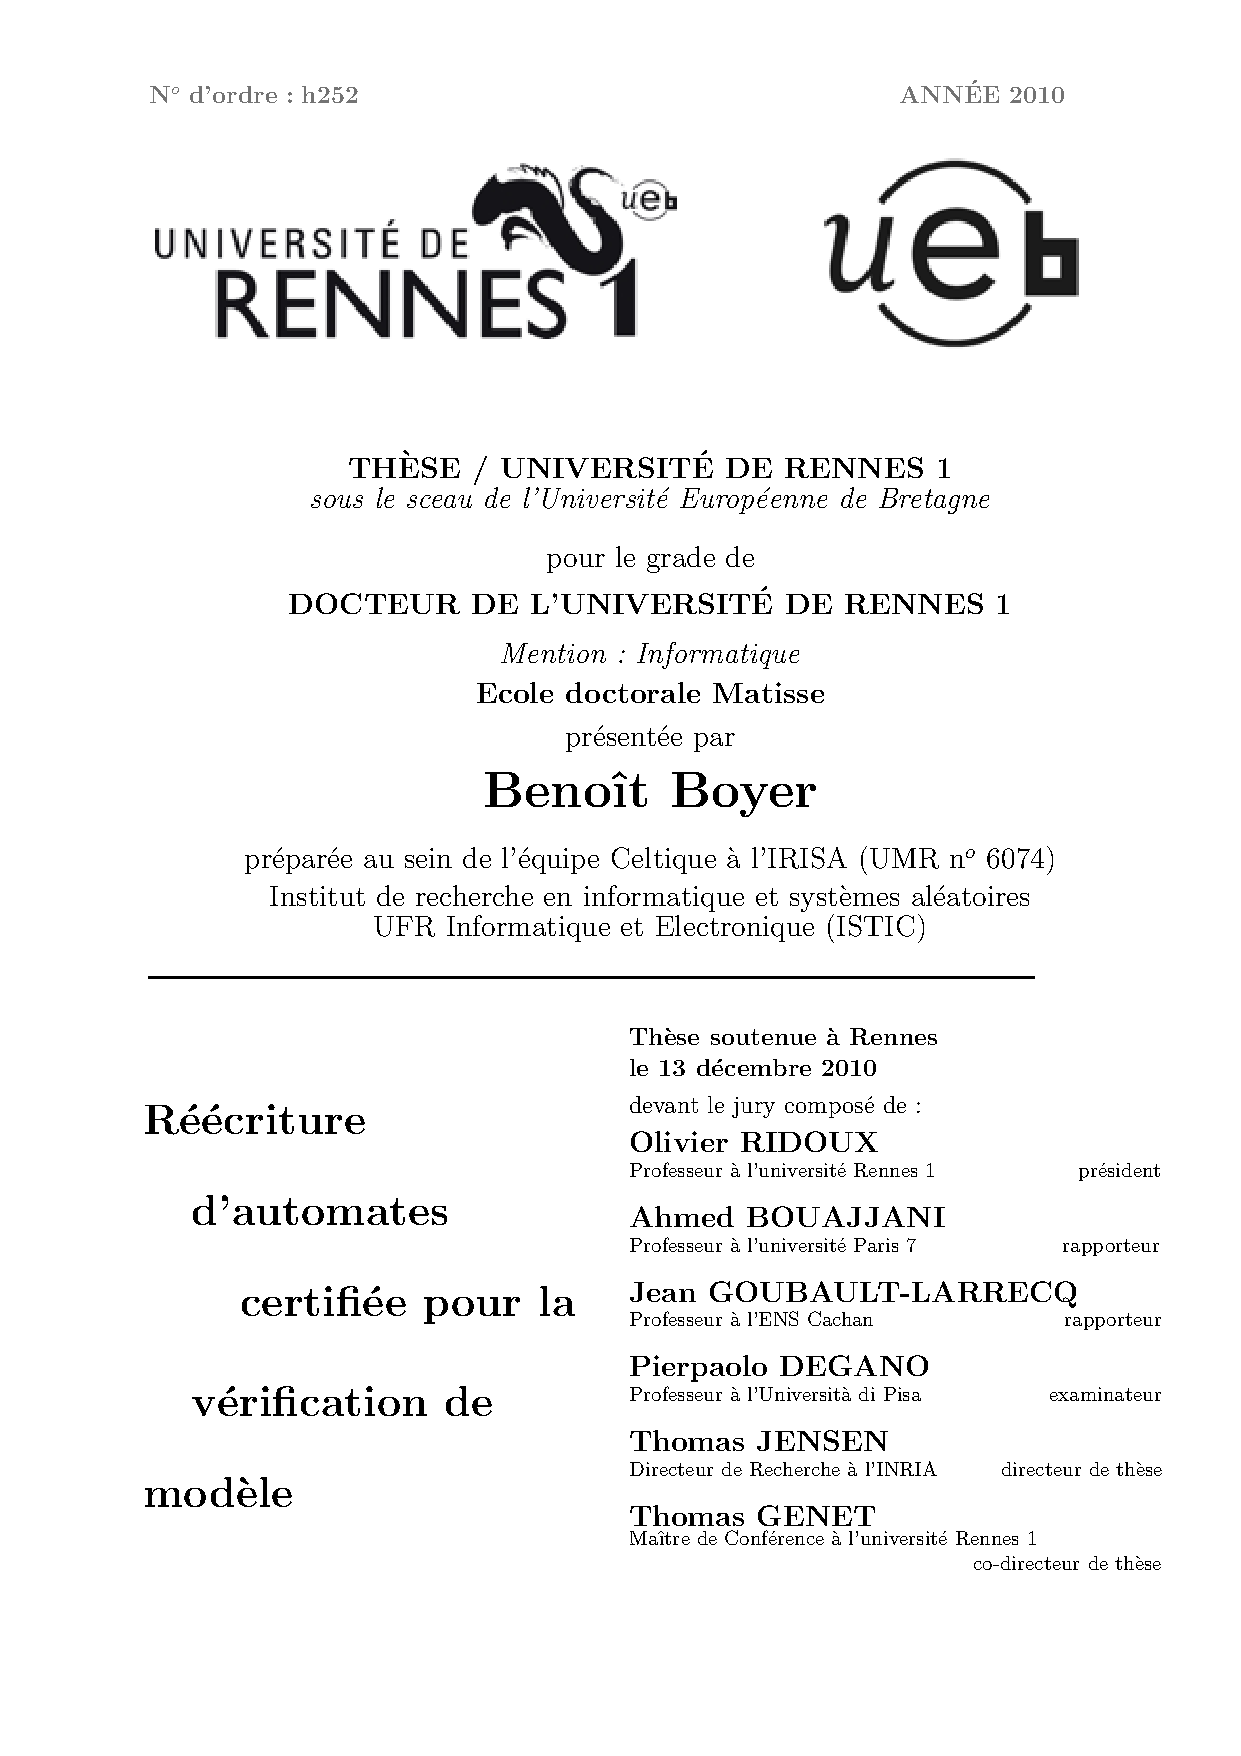
\includegraphics[width=20.4cm]{couverture/couverture}
\end{minipage}

%\title{La réécriture a-t-elle un sens ?!?}
%\title{De l'art de la quadrapilectomie appliquée à la réécriture!}
%\author{Un mec chevelu mais normal}
 \title{Réécriture d'automates certifiée pour la vérification de modèle}
 \author{Benoît \textsc{Boyer}}
 \date{\today}
 \maketitle
% \input{couverture/couverture}
\frontmatter
\tableofcontents
\mainmatter
\section*{Remerciements}

Quatre ans\dots\ quatre années à me supporter au gré d’une valse rythmée par les
accents d’euphorie ou d’enthousiasme succédées par des mouvements de
doute ou de déprime\dots Même si ce genre de phénomène est courant chez
les thésards, cela ne facilite pas l’encadrement pour autant ! C’est
donc pour cette raison que je tiens à remercier \textit{Thomas Genet} et \textit{Thomas
Jensen} d’avoir risqué l’aventure d’une thèse avec moi. Un contexte
scientifique est important, c’est indéniable, mais la qualité humaine
des relations est aussi un facteur incontournable pour
l’épanouissement d'un travail de recherche. J’ai trouvé cela dans
l’équipe-projet Lande, et plus encore dans l’équipe Celtique ! C’est
pour cette raison que je remercie tous les membres de l’équipe (\textit{David}, 
\textit{Thomas}, \textit{Frédéric}, \textit{Olivier}, \textit{Sandrine},
\textit{Laurent}, \textit{Florent}, \textit{Tiphaine}, \textit{Vincent},
\textit{Clément}, \textit{Pierre-Emmanuel}, \textit{Delphine}, \textit{Arnaud},
\textit{Najib}, \textit{Mattieu}, \textit{Florence}, et tous les autres !), 
avec qui nous avons pu échanger
scientifiquement, culturellement, humainement et passionnément lors de
nos pauses quotidiennes à la cafet’ de l’IRISA. Un autre point
marquant pour cette thèse : la collaboration avec \textit{Axel Legay} qui a
permis de nouvelles ouvertures et idées très intéressantes, et ce
d’autant plus, puisque cette collaboration perdure. Pour cela, je
remercie \textit{Axel}. Je porterai une attention toute particulière aux
rapporteurs de cette thèse, \textit{Jean Goubault-Larrecq} et \textit{Ahmed Bouajjani},
mais encore plus significativement à \textit{Jean Goubault-Larrecq}, pour la
patience et la minutie incroyables dont il a fait preuve dans ce
travail de relecture et de correction pour ce manuscrit. Il est parti
de loin, et le manuscrit a grandement profité de toutes ces remarques
: je l’en remercie vivement. Je remercie aussi l’ensemble du jury dont
\textit{Pierpaolo Degano} qui a accepté de faire le déplacement depuis
l’Université de Pise, ainsi que \textit{Olivier Ridoux} qui a présidé le
jury. L’expérience de l’enseignement à ses côtés fut indéniablement
novatrice et enrichissante et pour cela je l’en remercie ! Je remercie
ma famille et mes amis, pour la compréhension et le soutient dont ils
m’ont fait part ces derniers mois. En particulier, dans ces derniers
mois de rédaction dans l’urgence, où \textit{Manon} a accepté de s’endormir le
soir sans avoir vu son papa, et \textit{Soline} pour qui la charge de familiale
a pris plus d’importance et enfin \textit{Constance} qui elle est arrivée alors
que nous emménagions à Grenoble. À Toutes les trois, merci pour ces
moments de bonheur !



\chapter{Introduction}

\section{Pourquoi la vérification et la preuve de programmes?}

%Il est de fait complètement établi que la révolution informatique fut vue
L'informatique était vue comme la solution pour résoudre les problèmes de
fiabilité dans les domaines où toute défaillance 
opérationnelle peut conduire à des catastrophes. L'étymologie du mot {\em ordinateur}
est un bel exemple des espoirs que l'on a placés dans le domaine. Introduit par Jacques Perret
en 1955, il est issu du latin {\em ordinator} qui signifie celui qui met en ordre, qui règle
\footnote{\footnotesize Extrait de la définition d'{\em ordinator} dans le dictionnaire Gaffiot.}.
Cette définition omet de préciser que si l'ordinateur sait résoudre des problèmes, c'est 
grâce à l'ordonnateur (plus communément appelé programmeur ou développeur). %dont il 
L'ordinateur exécute les directives (le programme) du programmeur susceptibles de résoudre
les problèmes auxquels la machine est assignée. 
Si la machine est incontestablement meilleure que toute personne humaine dans la répétition 
intensive de calculs, l'introduction de l'informatique déplace simplement le problème 
de la fiabilité: le programme est-il suffisamment bien conçu pour permettre à l'ordinateur
de toujours réussir dans sa tâche? 

Si l'on se concentre sur la tâche du programmeur, celle-ci peut se résumer essentiellement
en deux étapes. Analyser le problème, puis si une méthode de résolution (au sens algorithmique du terme) existe,
la traduire en une spécification opérationnelle, le programme. Le {\em bug}\footnote{\footnotesize
  La terminologie française exacte est {\em bogue}.} intervient lorsqu'une faute 
de raisonnement conduit à une spécification erronée ou incomplète : conduisant l'ordinateur 
dans des comportements inattendus qui constituent les manifestations cliniques du bug.
Plus le problème à résoudre est complexe, plus il y a de risques de commettre une faute 
de conception conduisant à un bug lors de l'exécution du programme. 
De l'analyse du problème on peut aussi aboutir à une spécification dénotationnelle et formalisée à l'aide d'outils mathématiques.
Cette spécification "haut-niveau" est univoque et constituée de définitions et de propriétés simples:
la spécification dénotationnelle est souvent plus facile à comprendre que la spécification opérationnelle puisque 
débarrassée des aspects calculatoires.
On oblige les programmeurs à commenter leur code source pour une bonne raison. La spécification opérationnelle
étant peu compréhensible, il est nécessaire de donner au moins une spécification informelle pour qu'une personne autre
que le programmeur soit capable de comprendre le programme.

Une partie de la science informatique a pour unique but de rendre la conception de programmes
plus sûre. L'idée sous-jacente pour mener à bien cet objectif est de rapprocher 
la spécification opérationnelle d'une spécification dénotationnelle,
pour simplifier le plus possible la phase de conception que doit effectuer le programmeur.
C'est en partie le but recherché par les langages de programmation.
Ils se basent sur des logiques ou des paradigmes particuliers, qui peuvent se révéler plus ou moins
adaptés à certains types de problèmes algorithmiques. Au milieu des années 90, on recensait plus 
de 2000 langages~\cite{DOWEK-LANG}. Un langage de programmation repose 
sur un générateur (compilateur) ou un interprète (machine virtuelle) assurant la traduction automatique
du code source "haut-niveau" vers le code machine "bas-niveau".

Idéalement, on pourrait imaginer que la formalisation dénotationnelle soit suffisante
pour exprimer le programme à réaliser: par exemple un programme de tri est un programme
qui, à partir d'une liste, fournit une permutation de cette liste où les éléments sont
ordonnés. Cela reviendrait à ne donner que des définitions extensionnelles des programmes~\cite{DOWEK-LANG}.
Cependant, du point de vue du programmeur celles-ci ne sont pas assez expressives. 
Par exemple, alors qu'ils produisent le même résultat le tri à bulles et le tri rapide ne sont pas équivalents
d'un point de vue opérationnel.
% mais pas assez expressif: il est impensable pour tout bon programmeur de considérer comme équivalent le tri-rapide
% et le tri-à-bulles alors qu'ils produisent le même résultat une liste d'éléments triés.
A la place, on préfère utiliser une spécification dénotationnelle et vérifier à posteriori
que le programme est correct vis-à-vis de cette spécification. 
Un exemple commun est le système de types dans les langages de programmation. 
Lorsque le programme est correct,\textit{i.e.} si la vérification des types réussit,
on a l'assurance que le programme est sûr: 
les manipulations et les calculs qu'il effectue sont toujours réalisés sur des données
bien interprétées. Il n'y a pas de risque de confusion entre un entier et une adresse mémoire
(Un chou est un chou!~\cite{ASTERIX}).
Dans le cas des systèmes de types, la spécification dénotationnelle est facile à construire
car il s'agit d'annotations intégrées directement au langage. Pour exprimer
des propriétés plus fortes, on a souvent besoin d'un langage de spécification beaucoup
plus évolué qui prend place à côté du code source en commentaire (ex: JML pour Java) ou 
dans un fichier séparé.

Il est aussi possible de se passer d'une partie des  annotations dans certains langages modernes,
celles-ci pouvant être inférées automatiquement pour certaines vérifications.
Dans ce cas, une analyse automatique et statique (sans exécution) du programme
déduit automatiquement une spécification particulière, à partir de laquelle s'effectue la 
vérification. Certains types de propriétés peuvent être vérifiés de manière
complètement automatique.  Parmi les domaines qui fournissent des outils à l'analyse statique,
on peut citer les analyses utilisant la génération de contraintes sur les variables du programme, 
la théorie de l'interprétation abstraite~\cite{CousotC-POPL77} ou le model-checking~\cite{MC-Book}.
L'interprétation abstraite génère automatiquement une abstraction de l'ensemble des comportements possibles
du programme analysé pour des domaines particuliers. Le model-checking fournit aussi des outils d'analyses 
entièrement automatiques pour la vérification de propriétés temporelles mais suppose qu'une spécification opérationnelle
"haut-niveau" mais correcte du programme est fournie. 
Enfin, lorsque les propriétés sont trop difficiles à prouver automatiquement, on peut
faire appel à des assistants de preuves~\cite{Coq, Isa, Agda} qui permettent de construire interactivement 
des preuves correctes de programmes: le langage de l'assistant est assez expressif pour
exprimer le programme et ses propriétés. Des outils comme KeY~\cite{KEY} pour Java, Frama-C~\cite{FRAMAC} pour le C
génèrent à partir d'une spécification formelle et du code source d'un programme
des obligations de preuves que l'utilisateur doit prouver (soit à la main soit automatiquement)
afin d'assurer la correction du programme vis-à-vis de la spécification.

\section{La réécriture pour modéliser les programmes}

La réécriture est un modèle de calcul communément utilisé en informatique.
Elle formalise le calcul par des règles de transformation syntaxique pour des objets tels
que des mots ou des termes par exemple. 
Une règle de réécriture est un objet de la forme $l \rw r$.
La règle de réécriture s'applique à un objet $t$ si celui-ci contient une instance compatible
avec $l$ le membre gauche de la règle. Lorsque l'application est possible, on dit que $t$ se réécrit en un nouvel objet $t'$
que l'on obtient en remplaçant l'instance du membre gauche $l$ par l'instance du membre droit $r$ correspondante.
Mais on s'intéresse plus particulièrement à la réécriture de termes.
Un exemple courant est la définition des opérations élémentaires sur les entiers naturels suivant l'axiomatisation
de Peano: les termes sont alors définis par les opérateurs usuels $\_\ *\ \_$, $\_\ +\ \_$ sur les entiers naturels
représentés par $0 \in \Nat$ et $Sn \in \Nat$ qui représentent le successeur de l'entier $n \in \Nat$. Ainsi $SSS 0$
que l'on peut abréger par la notation $S^3 0$ correspond à l'entier naturel que l'on note plus volontiers $3$.
On peut définir la calcul de l'addition et de la multiplication, chacune par deux règles de la façon suivante :
\[
\textrm{ Addition :}\left\{
\begin{array}{l}
  0 + x \rw x\\
  S x + y \rw x + S y
\end{array}\right.
\quad
\textrm{ Multiplication :}\left\{
\begin{array}{l}
  0 * x \rw 0\\
  S x + y \rw (x * y) + x
\end{array}\right.
\]
Les variables $x$ et $y$ peuvent être remplacées par n'importe quel terme, pour constituer l'instance du membre gauche
d'une règle de réécriture. Par exemple le terme $t = SS0 + SS0$ constitue une instance du membre gauche de la règle
$S x + y \rw x + S y$ en posant $x = S0$ et $y = SS0$: on peut donc réécrire $t$ en $t' = S0 + SSS0$. 
A contrario, $t$ et $t'$ ne contiennent pas d'instance pour appliquer la règle $0 + x \rw x$.
En répétant successivement les étapes de réécriture, on obtient la chaîne de réécriture suivante:
\[ SS0 + SS0 \lrw S0 + SSS0 \lrw 0 + SSSS0 \lrw SSSS0 \]
La transformation syntaxique de $SS0 + SS0$ en $SSSS0$ correspond au résultat attendu pour l'opération $2$ "plus" $2$ 
qui est égal à $4$.

\newcommand{\fib}{\mathit{fib}}

L'expressivité des systèmes de réécriture permet de modéliser plus que l'arithmétique. 
En particulier tout système calculatoire peut-être modélisé, dont les programmes informatiques
par exemple. En fait, certains langages de programmation comme \ocaml~\cite{OCAML} ou \tom~\cite{TOM}
intègrent nativement la réécriture. L'exemple suivant donne un codage de la
célèbre\footnote{\footnotesize au moins chez les mathématiciens et les cuniculiculteurs.} fonction de Fibonacci.
On note par $\fib(n)$ le nombre de Fibonacci de rang $n$. En reprenant et complétant la formalisation des entiers
naturels précédente, on peut définir la fonction $\fib(n)$ de la manière suivante:
\[
\begin{array}{l}
  \left\{\begin{array}{l}
      0 \le y \rw true\\
      Sx \le Sy \rw x \le y\\
      Sx \le 0 \rw \false
    \end{array}\right.
  \hspace*{4cm}
  \left\{\begin{array}{l}
      x - 0 \rw x\\
      Sx - Sy \rw x - y\\
      0 - Sy \rw \bottom
    \end{array}\right.\\
  \\\\
  \left\{\begin{array}{l}
      \ifte(\true, x, y) \rw x\\
      \ifte(\false,x, y) \rw y
    \end{array}\right.\\\\
  \hspace*{1.2cm}\fib(x) \rw \ifte(x\le S0, S0, \fib(x - S0) + \fib (x - SS0))
\end{array}
\]

\section{Vérification de systèmes de réécriture}

On peut remarquer que la définition de la fonction utilise la définition de la soustraction qui n'est que partiellement
définie, ce que l'on symbolise ici par la réécriture en $\bottom$. On peut donc se demander si la fonction $\fib$ 
est correctement définie pour tout $n \in \Nat$, c'est à dire qu'elle ne produit jamais le terme
$\fib(\bottom)$ correspondant simplement à un plantage du programme.

Une manière de vérifier que le système de réécriture n'engendre pas le terme $\fib(\bottom)$ est de générer tous les 
termes que peut produire le système de réécriture. 
Pour cela on peut décider de représenter l'ensemble des termes initiaux $\fib(n)$, correspondant à l'ensemble des valeurs 
puis de calculer l'ensemble des termes que l'on peut obtenir, qui correspondent finalement à l'ensemble des valeurs
possibles que peut prendre le programme. La technique consiste à compléter itérativement l'ensemble $I$, 
par les nouvelles valeurs que peut prendre la fonction jusqu'à ce l'ensemble soit saturé. On note cet ensemble $\R^*(I)$
c'est à dire l'ensemble des termes atteignables par réécriture des termes initiaux.

\begin{figure}[ht!]
  \centering
  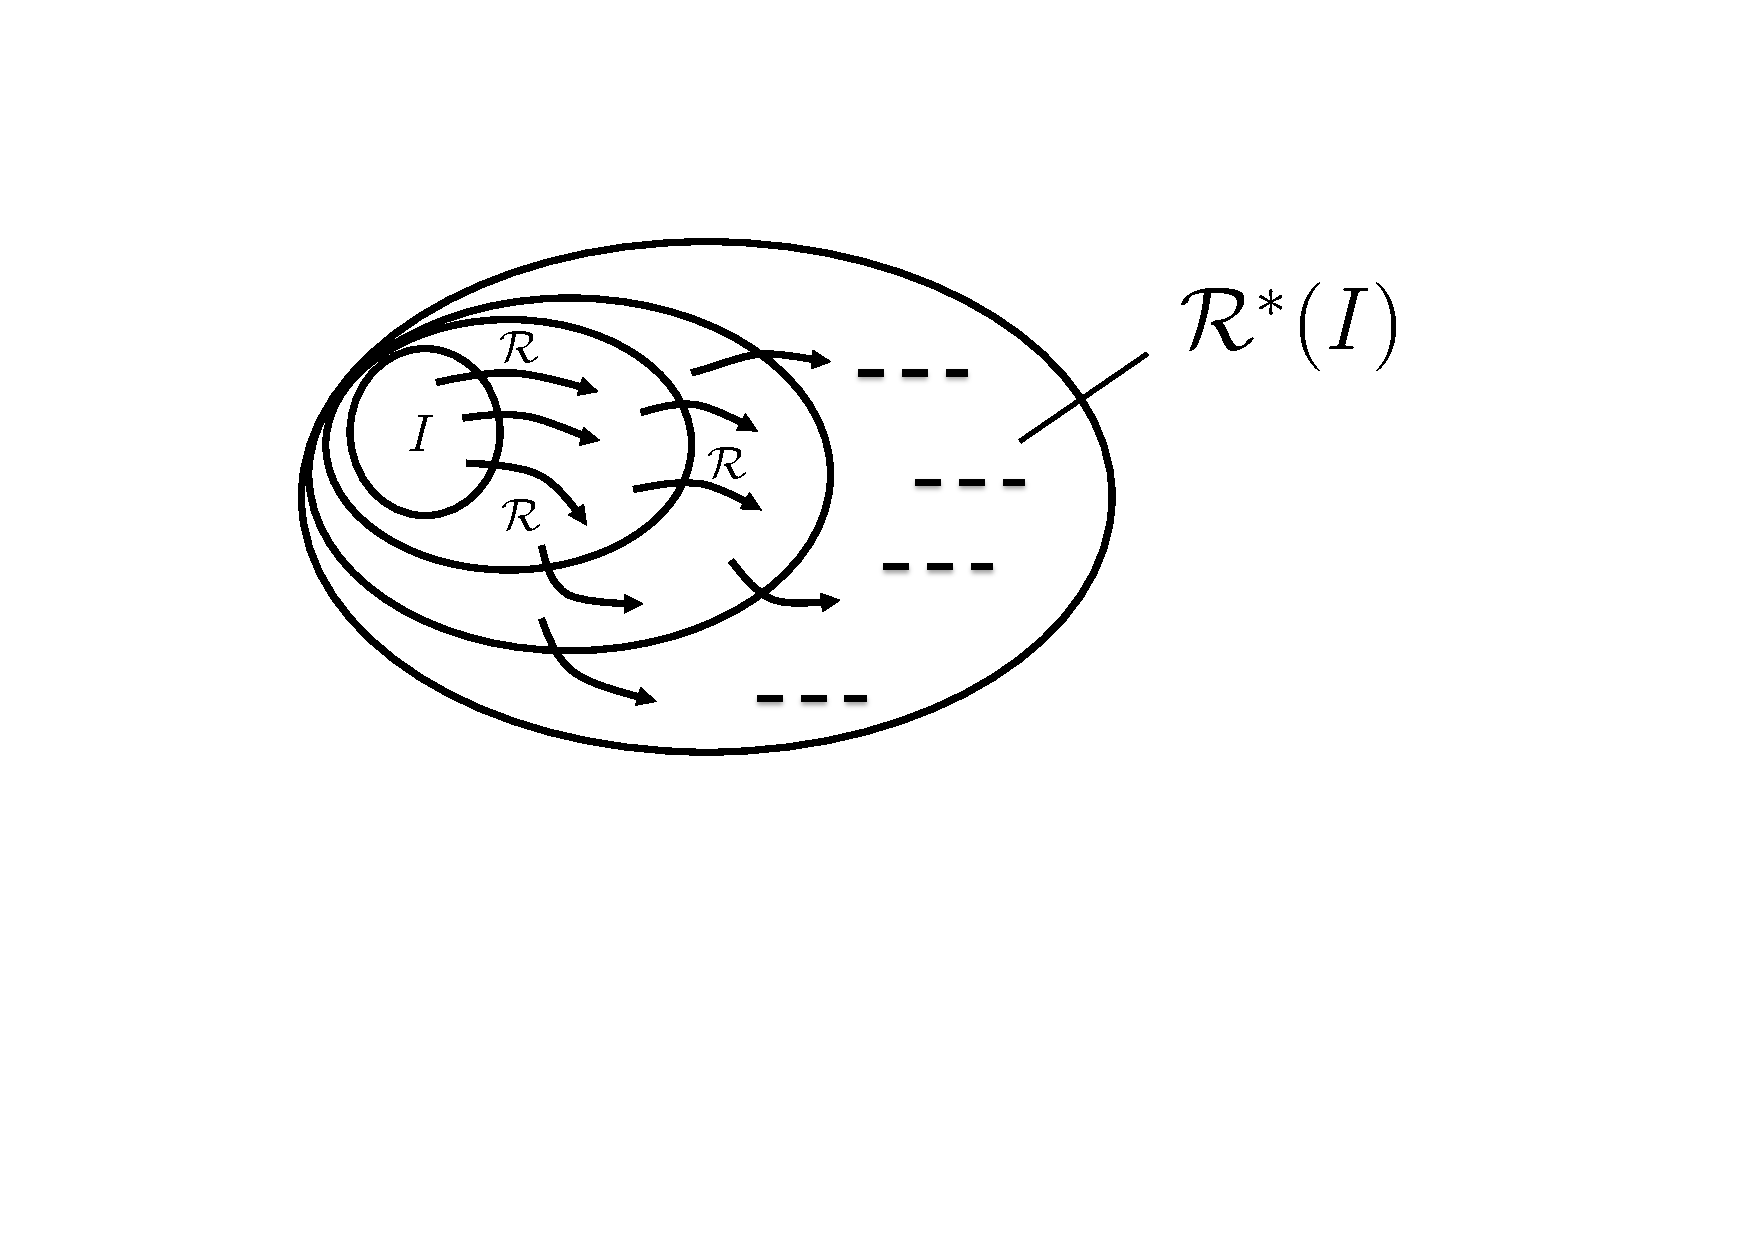
\includegraphics[width=12cm]{1_intro/exact}
\end{figure}

En supposant que l'on sache calculer $\R^*(I)$, on est alors à même de vérifier que le terme $\fib(\bottom)$
n'est jamais produit. C'est ce que l'on appelle communément le problème d'atteignabilité.

Mais plusieurs problèmes doivent être résolus pour être capable de
calculer $\R^*(I)$.  L'ensemble des termes initiaux peut être infini,
comme c'est d'ailleurs le cas pour la fonction de Fibonacci.  Il faut
donc fournir une représentation finie d'un ensemble infini.  Les
automates d'arbres sont une approche tout à fait indiquée pour
résoudre ce problème sur les termes.  Cependant, tout ensemble de
termes n'est pas représentable par un automate d'arbres.  Et c'est
souvent le cas de l'ensemble des états accessibles d'un programme, et
des termes atteignables d'un système de réécriture qui le
modélise. On peut en déduire qu'il n'existe pas toujours d'automate
d'arbres capable de représenter l'ensemble des termes
atteignables. En fait, de manière plus générale, il n'est pas possible
de calculer (et de représenter) l'ensemble des termes atteignables
pour un système de réécriture donné.  Par contre, il est possible d'en
calculer une sur-approximation.  C'est l'objectif de la complétion
d'automates d'arbres : compléter le langage\footnote{\footnotesize
  l'ensemble des termes représenté par l'automate.} d'un automate
d'arbres en ajoutant successivement les termes atteignables.  C'est un
semi-algorithme introduit par Th.~Genet~\cite{Genet-RTA98}, qui
calcule un automate $\aapprox$ caractérisant une sur-approximation
d'un ensemble $\R^*(I)$.  Lorsqu'il n'est plus possible de compléter
l'automate, ce dernier est clos par réécriture, c'est à dire qu'il
contient tous les termes atteignables.  L'approximation est paramétrée
par $E$ un ensemble d'égalités (ou équations) qui définissent des
classes d'équivalence qui permettent des raccourcis syntaxiques.  Par
exemple, on peut définir les équations $x + y = y + x$ pour définir la
commutativité de l'addition ou $Sx = SSx$ pour considérer tout entier
(sauf $0$) équivalent à son successeur: on partitionne alors les
entiers en deux classes $\dot{0}$ et $\dot{1}$.  La complétion est un
semi-algorithme, car si l'ensemble d'équations ne construit pas des
classes d'équivalence assez fortes, alors le calcul diverge.

\begin{figure}[ht!]
  \centering
  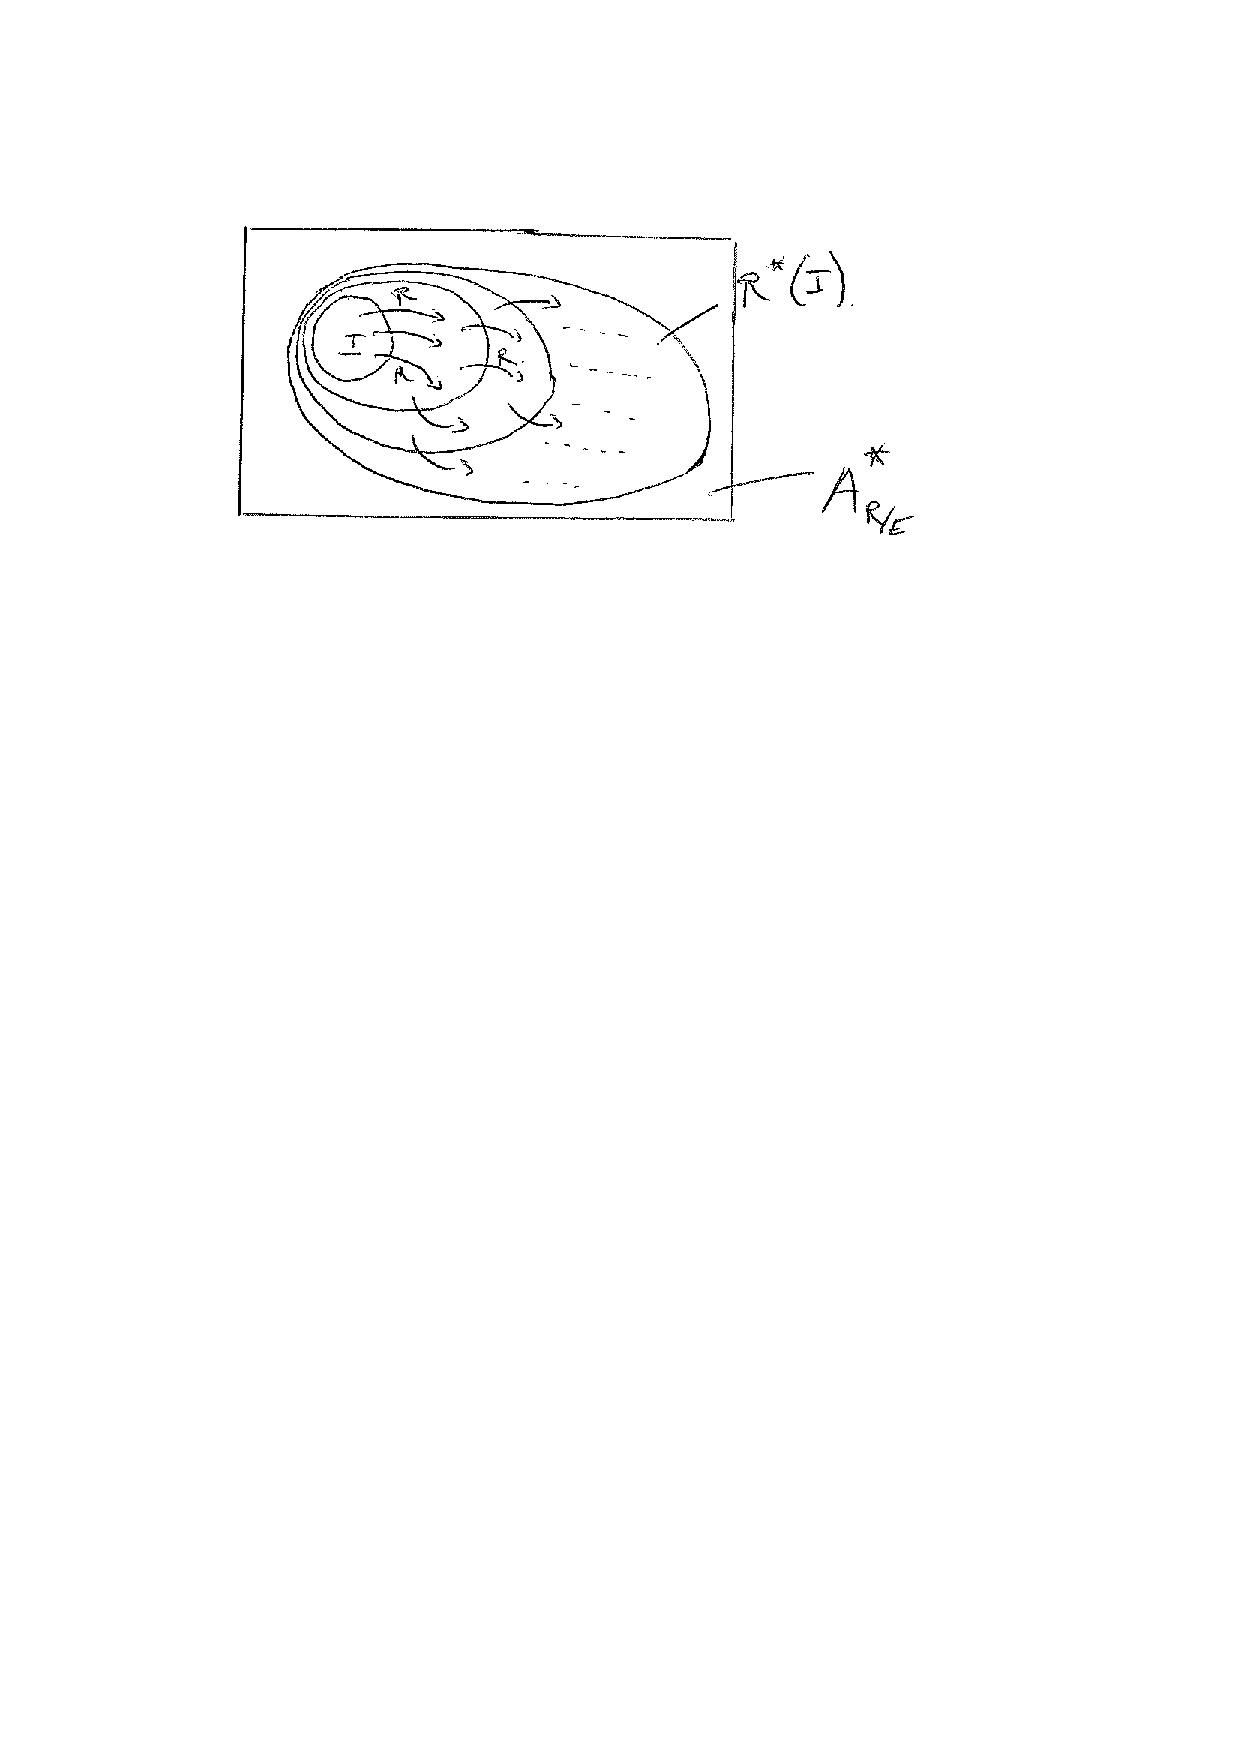
\includegraphics[width=12cm]{1_intro/approx}
\end{figure}

Du point de vue du problème d'atteignabilité, calculer une sur-approximation reste correct: en effet, si le terme $\fib(\bottom)$ 
n'est pas dans la sur-approximation de $\desc(I)$ alors il n'est clairement pas dans $\desc(I)$
non plus. Par contre, si la vérification échoue on ne peut rien dire.
L'outil \timbuk~\cite{timbuk} implémente l'algorithme de complétion et permet de vérifier des propriétés
de sûreté sous forme de problème d'atteignabilité. Il est utilisé principalement dans la
vérification des protocoles cryptographiques. Il se base sur une spécification symbolique 
et opérationnelle du système à vérifier, c'est à dire un système de réécriture où les termes sont les états possibles
du protocole, et les règles de réécriture modélisent les transitions du protocole.
Il fonctionne suivant le principe illustré ci-dessus.
Plus récemment, il a été montré qu'il est possible de modéliser un sous-ensemble important du ByteCode Java
par un système de règles de réécriture~\cite{BoichutGJL-RTA07}. Les termes du systèmes représentent les états
de la machine virtuelle Java, et les règles de réécriture la sémantique de Java. L'outil Copster~\cite{Copster} 
génère à partir d'un fichier \texttt{.class} le système de réécriture: l'exécution du système de réécriture 
correspond exactement à l'exécution du programme Java. 



\section{Présentation des contributions de cette thèse}
Les contributions de cette thèse trouvent leur place dans le cadre de vérification de programmes Java
compilés en systèmes de réécriture et dont l'analyse se base sur la complétion d'automates d'arbres.
La complétion a pour ambition de proposer une technique intermédiaire entre la preuve de programme
entièrement réalisée à la main, et les outils d'analyse statique.
Ces derniers, bien qu'ils soient complètement automatiques, présentent le défaut de ne traiter que 
certains types de propriétés reposant sur une théorie qui est décidable, comme l'interprétation abstraite et le model-checking.
La complétion permet de définir un cadre de vérification semi-automatique grâce à une abstraction
régulière paramétrable en fonction de l'analyse et des propriétés à vérifier.
La seule intervention dans le processus d'analyse reste la construction de l'ensemble d'équations
qui peuvent être générées automatiquement ou fournies directement à la main. Dans ce dernier cas, 
le degré d'expertise requis est toujours moins important que celui nécessaire à la preuve de programme
entièrement manuelle. D'autre part, l'approximation calculée est toujours correcte, quelle que soit l'abstraction choisie.
%ce qui n'a pas besoin d'être démontré pour chaque nouveau domaine. 
% A l'opposé, on trouve les assistants de preuves permettant
% la spécification et la construction de preuves de programmes à la main. Cette approche a le défaut
% d'être extrêmement coûteuse en temps et requiert un important niveau d'expertise dans la preuve de programme en général. 
% Les analyses basées sur la complétion d'automates d'arbres tente de s'intercaler entre ces deux univers
% en tant qu'outil de vérification semi-automatique. 
% En effet, l'analyse est basée sur un calcul sur-approchant tous les comportements du systèmes, 
% dont l'approximation est facilement paramétrable.
Les travaux de cette thèse ont pris place dans le projet de l'ANR Ravaj~\cite{RAVAJ}.
Les objectifs du projet portaient notamment sur l'adaptation de la complétion à l'analyse d'applications Java
et la certification des analyses effectuées. 
% Plusieurs objectifs ont été soulevés dans ce projet comme l'adaptation de la technique de complétion
% afin de réaliser ce type d'analyse d'une part, mais aussi l'aspect certification de l'analyse dans le
% but d'obtenir un degré de confiance élevé dans la technique proposée. 
En cours de projet, deux autres objectifs se sont dégagés comme le passage à l'échelle,
mais aussi le besoin d'étendre les propriétés vérifiables à la logique temporelle.
% L'outil \timbuk\ %qui est l'implémentation initiale
% était initialement destiné à la vérification de protocoles cryptographiques. 
% Pour les protocoles, les systèmes de réécriture sont de petite taille et la définition d'abstraction 
% réclame une expertise pointue mais réaliste.
Dans le cas des programmes en ByteCode Java, la taille des systèmes de réécriture est trop importante
pour espérer construire à la main une bonne abstraction. La première contribution de cette thèse est de
proposer une technique de raffinement automatique d'approximation
afin de réduire l'expertise nécessaire à la définition des équations.
La deuxième contribution étend les propriétés vérifiables par la complétion aux propriétés temporelles.
Enfin la troisième contribution est de certifier les analyses effectuées.



\bigskip
\subsection*{Le raffinement automatique} 
L'objectif du chapitre~3 de cette thèse est de montrer comment étendre la complétion
aux techniques de raffinement automatique de l'abstraction. Fournir une abstraction permettant à la complétion
de terminer est faisable même pour les programmes Java. Le problème est de fournir une abstraction qui soit assez
fine pour vérifier la propriété attendue, tout en assurant la terminaison. Sous ces contraintes, quel que soit
le niveau d'expertise, il est à peu près impossible de définir à la main la bonne abstraction. Le raffinement automatique
de l'abstraction permet de simplifier cette tâche: on peut alors définir une abstraction peu précise mais qui assure
la terminaison du calcul, l'abstraction étant affaiblie automatiquement lorsque c'est nécessaire en suivant une approche à la "CEGAR".
La contribution de ce chapitre est double. Tout d'abord, elle offre à la complétion la possibilité de
construire des contre-exemples. Cette fonctionnalité, bien qu'indispensable, était absente et difficile à mettre
en place dans le formalisme d'origine. Ensuite, on propose un algorithme de raffinement, non pas basé 
sur une tabulation des étapes de calculs et sur des calculs arrières qui peuvent s'avérer coûteux, mais sur un élagage 
original de l'automate construit. 
% On propose d'étendre la complétion d'automates d'arbres afin de détecter les cas où l'abstraction se
% trouve justement trop grossière, ainsi qu'une technique de raffinement basée sur l'élagage de l'automate.
% L'apport est double car la procédure de raffinement permet une détection systématique lorsque le programme viole
% la propriété attendue.

Ce chapitre est actuellement en cours de soumission.% à la conférence~TACAS~2011.

\bigskip
% La seconde contribution de cette thèse s'intéresse à étendre le type de propriétés prouvables par la complétion.
\subsection*{La vérification comportementale}
Le chapitre~4 montre comment la complétion d'automates d'arbres peut être utilisée afin de vérifier 
des propriétés temporelles sur le graphe d'appels des méthodes d'un programme Java. Il est difficile 
de montrer des propriétés avec une composante temporelle en se basant uniquement sur la vérification du
problème d'atteignabilité. Une propriété comme 
"{\em si l'utilisateur clique sur le bouton Non, alors la requête ne sera pas émise sur le réseau}" est un exemple
des propriétés que l'on souhaiterait prouver sur des programmes Java. Dans ce chapitre, on montre comment tirer partie
de l'information contenue dans l'automate. %La complétion construit des automates qui contiennent naturellement une abstraction de la relation de réécriture. 
Cette abstraction de la réécriture correspond à une abstraction 
de l'exécution du programme qui induit notamment la construction explicite du graphe d'appels des méthodes Java.
On montre comment extraire cette information de l'automate complété, et comment utiliser les techniques standard
de vérification issues du model-checking, ce qui permet de vérifier des propriétés en logique temporelle~LTL.

Les travaux du chapitres~4 ont été présentés lors du workshop~Rule'09~\cite{BoyerG-RULE09}.

\bigskip
\subsection*{La certification de la complétion}
Le chapitre~5 décrit les travaux réalisés dans l'assistant de preuves \coq\ pour certifier la
complétion d'automates d'arbres. L'outil \timbuk\ a été notablement optimisé, et par ailleurs, différentes implémentations 
ont vu le jour. Certaines de ces implémentations n'utilisent plus les automates d'arbres au niveau algorithmique mais uniquement
comme format d'entrée du problème et comme format de sortie pour le résultat. %n'utilisent plus les automates d'arbres que pour produire le résultat final.
Par conséquent, ces outils sont de plus en plus éloignés de la spécification originale
de l'algorithme. Les optimisations sont une source de bugs supplémentaires, généralement difficiles à repérer.
% Les bugs loin d'être absents sont souvent durs à identifier:
% les optimisations sont une source de bugs car elles peuvent introduire des cas particuliers qui peuvent être 
% difficiles à repérer à l'origine des bugs. 
D'autre part, les implémentations %récentes étant plus performantes, elles 
sont capables de traiter des problèmes de taille beaucoup plus importante. Comme le résultat est non vérifiable à la main,
il est difficile de se convaincre de sa correction. L'ensemble de ces constats a permis de conclure qu'il était nécessaire de
vérifier les résultats de ces outils, de manière à obtenir une preuve \coq\ de la validité des résultats. C'est le rôle que joue
le vérificateur certifié en \coq. A partir d'une spécification de la réécriture et des automates d'arbres en \coq, on formalise
la correction d'un automate point fixe par rapport au problème d'atteignabilité. On montre ensuite comment vérifier la propriété
en \coq, ce qui définit le vérificateur. Ensuite, il est possible d'extraire puis de compiler un vérificateur 
conforme à la spécification \coq. Celui-ci permet de vérifier la validité de chaque résultat obtenu par un des outils
qui implémentent la complétion.

Le chapitre~5 a aussi fait l'objet d'une publication lors de la conférence IJCAR'08~\cite{BoyerGJ-IJCAR08}.

%En vérification 
%%% Local Variables: 
%%% mode: latex
%%% TeX-master: "../main"
%%% End: 


\chapter{Prérequis}
\label{chap:preliminaires}

Ce chapitre a pour ambition de rappeler les bases nécessaires pour la théorie de la réécriture,
des automates d'arbres, et présente le cadre de la vérification de modèles symboliques auquel
nous nous intéressons dans cette thèse. Pour plus détails, le lecteur pourra trouver plus d'informations
sur la réécriture dans~\cite{BaaderN-book98} et dans~\cite{TATA} pour les automates d'arbres.


\section{Termes et réécriture}

\begin{definition}
  Une \textbf{signature} $\F$ est un ensemble de symboles de fonctions dont l'arité est fixée par
  une fonction $\phi : \F \rw \N$. Par $\F_i$, on distingue l'ensemble des symboles $ f \in \F$
  d'arité $\phi(f) = i$. Dès lors, $\F_0$ caractérise l'ensemble des \textbf{constantes}.
\end{definition}


\begin{definition}
  Soit $\F = \{ f_2, g_1, h_2, \dots\}$ une signature\footnote{\footnotesize Pour définir rapidement $\F$, Chaque symbole est indicé par son arité}.
  Soit $\X$ un ensemble de \textbf{variables} tel que $\X \cap \F = \emptyset$.
  L'ensemble $\TFX$ dénote l'\textbf{algèbre de termes} engendrée par la signature $\F$ à partir de $\X$. On définit $\TFX$ comme le plus petit ensemble
  tel que:
  \begin{itemize}
  \item $\X \subseteq \TFX$ 
  \item pour tout $n \in \N$ et $f \in \F_n$, si $t_1, \dots, t_n \in \TFX$ alors $f(t_1, \dots, t_n) \in \TFX$
  \end{itemize}
\end{definition}
Les éléments de $\TFX$ sont appelés des \textbf{termes}. On note $\TF$, l'algèbre des \textbf{termes clos} -- \textit{i.e.} 
sans variable -- ce qui correspond à $\T(\F,\emptyset)$. %est engendrée à partir de $\X = \emptyset$.
Cette définition inductive nous indique que toute variable est un terme, 
et que l'application d'un symbole de fonction à des termes engendre de nouveaux termes. Cette construction permet de voir
les termes comme des arbres étiquetés.
Considérons $\F = \{ f_3, g_2, h_1 \}$ et $\X = \{x, y, z\}$. On peut alors construire le terme $f(g(x,h(y)), g(x, g(y, z)), h(x))$
que l'on peut représenter par l'arbre de la figure~\ref{fig:terme-arbre}.

\begin{figure}[ht!]
  \centering
  \begin{tikzpicture}[level distance=12mm]
    \tikzstyle{level 1}=[sibling distance=20mm]
    \tikzstyle{level 2}=[sibling distance=12mm]
    \node{$f$}%[grow=right]
    child{node{$g$}
      child{node{$x$}
        edge from parent node[left] {\tiny $1$}
      }
      child{node{$h$}
        child{node{$y$} edge from parent node[right] {\tiny $1$}}
        edge from parent node[right] {\tiny $2$}
      }
      edge from parent node[left] {\tiny $1$}
    }
    child{node{$g$}
      child{node{$x$}
        edge from parent node[left] {\tiny $1$}
      }
      child{
        node{$g$}
        child{node{$y$} edge from parent node[left] {\tiny $1$}}
        child{node{$z$} edge from parent node[right] {\tiny $2$}}
        edge from parent node[right] {\tiny $2$}
      }
      edge from parent node[left] {\tiny $2$}
    }
    child{node{$h$}
      child{node{$x$} edge from parent node[right] {\tiny $1$}}
      edge from parent node[right] {\tiny $3$}
    };
  \end{tikzpicture}
  \caption{\footnotesize le terme $f(g(x,h(y)), g(x, g(y, z)), h(x))$ vu comme un arbre étiqueté}
  \label{fig:terme-arbre}
\end{figure}

La représentation d'un terme sous forme d'arbre permet de voir
facilement que le terme $f(g(x,h(y)), g(x, g(y, z)), h(x))$ est constitué des \textbf{sous-termes}
représentés par les sous-arbres dans la figure~\ref{fig:terme-arbre}.
Ainsi $g(x, g(y, z))$ est un sous-terme de $f(g(x,h(y)), g(x, g(y, z)), h(x))$.
Un sous-terme est caractérisé par sa position à partir de la racine du terme
qui le contient. Une \textbf{position} $p$ est définie comme un \textbf{mot de $\NN$} qui correspond
à un chemin dans l'arbre. Le mot vide $\epsilon$ correspond à la racine du terme.

\begin{definition}
  Soit un terme $t \in \TFX$. L'ensemble $\pos(t)$ des positions de $t$ se définit inductivement
  comme:
  \begin{itemize}
  \item $\pos(t)= \{ \epsilon\} $ si $t \in \X$
  \item $\pos(f(t_1,\dots,t_n)) = \{ \epsilon \} \cup \{i.p \mid 1 \leq i \leq n
    \et p \in \pos(t_i) \}$
  \end{itemize}
\end{definition}


Si $p \in \pos(t)$, alors $t|_p$ dénote le \textbf{sous-terme de} $t$ \textbf{à la position} $p$ et
$t[s]_p$ dénote le terme obtenu après le \textbf{remplacement} du sous-terme $t|_p$ par le terme $s$.
On peut les définir par induction sur $p \in \pos(t)$:
\begin{itemize}
\item $t|_\epsilon = t$
\item $f(t_1,\dots, t_n)|_{i.p} = t_i|_p$
\end{itemize}
et
\begin{itemize}
\item $t[s]_\epsilon = s$
\item $f(t_1,\dots, t_n)[s]_{i.p} = f(t_1,\dots, t_i[s]_p,\dots,t_n)$
\end{itemize}

\begin{definition}
  L'ensemble des variables d'un terme $t \in \TFX$ est dénoté par $\vars(t)$ et se définit simplement
  comme $\vars(t) = \{ x \in \X \sep \exists p \in \pos(t) \st x = t|_p\}$
\end{definition}
On remarque pour tout terme $t \in \TFX$, $\vars(t) = \emptyset$ alors $t$ est un terme clos, ce qui est équivalent à $t \in \TF$.

\begin{definition}
  Une \textbf{substitution} est une fonction $\sigma$ de $\X$ vers $\TFX$, telle que 
  pour un ensemble fini de variables $x \in X$ on a $x \not= \sigma(x)$. Cet
  ensemble constitue le domaine de la fonction $\sigma$ que l'on note $\dom(\sigma)$.
  On étend les substitutions à des endomorphismes de $\TFX$. 
  On note alors $t\sigma$ (ou $t.\sigma$) l'application de la substitution $\sigma$ au terme $t$ 
  qui remplace toute occurrence des variables par leur image respective via $\sigma$:
  \begin{itemize}
  \item $t\sigma = \sigma(t)$ lorsque $t \in \X$
  \item $f(t_1, \dots, t_n)\sigma = f(t_1\sigma, \dots, t_n\sigma)$
  \end{itemize}
\end{definition}
On appelle $id$, la substitution dont le domaine $\dom(\sigma)$ est vide.
Pour tout terme $t \in \TFX$, on a $t.id = t$.

On dit qu'un terme $t$ est une \textbf{instance} d'un terme $s$ lorsqu'il existe une substitution
$\sigma$ telle que $t = s\sigma$.

Un système de règles de réécriture -- TRS en abrégé
\footnote{\footnotesize abréviation issue de la formulation anglaise équivalente {\em term rewriting system}} -- 
$\R$ est un ensemble de règles de réécriture. 

\begin{definition}
  Une \textbf{règle de réécriture} est un couple, notée $l \rw r$, composée de deux termes $l, r \in \TFX$,
  telle que $l \not \in \X$, et $\var(l) \supseteq \var(r)$. 
  On appelle $l$ et $r$ respectivement le membre gauche et le membre droit de la règle.
  Une règle de réécriture est \textbf{linéaire à gauche} (ou à droite) si chaque variable de $\X$ 
  n'apparaît pas plus d'une fois dans son membre gauche (droit {\textit resp.}).
  %Une règle est \textbf{linéaire} si elle est à la fois linéaire à gauche et à droite.
\end{definition}

Un système de règles de réécriture est linéaire à gauche (ou à droite) si chacune 
de ses règles est linéaire à gauche (à droite {\textit resp.}). De même, le système est 
linéaire si il est linéaire à gauche et à droite.

\begin{definition}
  Si $\R$ est un TRS, alors on note $\rw_{\R}$ la relation de réécriture qu'il induit sur les termes.
  On dit que le terme $s$ se réécrit en $t$ par la règle $l \rw r \in \R$ si et seulement si l'un des sous-termes de $s$
  est une instance de $l$ et $t$ est le terme $s$ où l'instance de $l$ est remplacée par l'instance de $r$ correspondante:

  \noindent $s \rw_\R t \equ$
  \begin{flushright}
    $\exists\ l \rw r \in \R,\ p \in Pos(s),\ \sigma: \X \rw \TFX \textrm{ tels que }\quad \quad \quad$
    $s|_p = l\sigma \quad \et \quad  t = s[r\sigma]_p$
  \end{flushright}
\end{definition}
Ainsi, la règle $g(x, y) \rw y$ permet de réécrire le terme $h(g(x, g(y, z)))$ 
soit en $h(g(x, z))$ ou $h(g(y, z))$, suivant que l'on choisisse de réécrire le sous-terme
à la position $1.2$ ou à la position $1$.

La clôture transitive et réflexive de $\rw_\R$ se note $\rw^*_{\R}$.
Si $A$ est un ensemble de termes clos, on définit l'ensemble des $\R$-descendants 
de $A$ comme $\desc(A) = \{t \in \TF \sep \exists s \in A \st s \rw^*_{\R} t \}$.

\begin{definition}
  Une \textbf{équation} est un couple, notée $s = t$, composée de deux termes $s, t \in \TFX$.
  Si $e$ est l'équation $s = t$, alors deux termes $u$ et $v$ sont égaux modulo $e$ si et seulement si
  
  \noindent $u =_e v \equ$\\
  \[\exists\ \sigma: \X \rw \TFX \textrm{ telle que } \quad s = u\sigma \quad \et \quad  t = v\sigma\]
  
  Si $E$ est un ensemble d'équations, on note $=_E$ la relation d'équivalence définie comme la plus petite relation
  de congruence contenant la relation $\{ u =_E v \sep \exists e \in E,\ u =_e v\}$
\end{definition}


\begin{definition}
  Soient $\R$ un TRS, et $E$ un ensemble d'équations. On définit la \textbf{réécriture modulo} comme la relation
  $\rw_\RE$ définie comme:
  \[\forall\ s, t \in \TFX,\quad s \rw_\RE t \equ \exists u, v \in \TFX,\quad s =_E u \rw_\R v =_E t\]
\end{definition}
De la même manière que pour $\R$, on note $\rw_\RE^*$ la clôture transitive et réflexive de $\rw_\RE$, et 
on définit l'ensemble des $\RE$-descendants pour un ensemble $A$ de termes clos par
$\descE(A) = \{t \in \TF \sep \exists s \in A \st s \rw^*_{\RE} t \}$.

%\comments{Paires critiques ou pas???}
\section{Les automates d'arbres}
\label{sec:automates}

Soit $\Q$ un ensemble fini de constantes appelées \textbf{états} tel que $\Q \cap \F= \emptyset$.
On définit $\TFQ$ l'algèbre engendrée par $\F$ et $\Q$, que l'on appelle l'ensemble des \textbf{configurations}.

\begin{definition}%[Les transitions]
  \label{def:transitions}
  Dans un automate d'arbres, une \textbf{transition} est une règle de réécriture de la forme $c \rw q$, où $c$ est une configuration
  \textit{i.e.} $c \in \TFQ$ et $q \in \Q$ est un état. On distingue deux sortes de transitions dans un automate d'arbres:
  \begin{itemize}
  \item Une \textbf{transition normalisée} est une transition de la forme $f(q_1, \dots, q_n) \rw q$
    avec $f \in \F_n$, et $q_1, \ldots, q_n, q \in \Q$ sont des états
  \item Une \textbf{$\varepsilon$-transition} est une transition de la forme $q' \rw q$ où $q', q \in \Q$ sont des états
  \end{itemize}
\end{definition}

% An epsilon transition is a transition of the form $q \f q'$ where $q$ and $q'$
% are states. Any set of transition $\Delta \cup \{q \f q'\}$ can be
% equivalently replaced by $\Delta \cup \{c \f q' \sep c \f q \in \Delta \}$.

\begin{definition}% [Bottom-up nondeterministic finite tree automaton]
  Un automate d'arbres ascendant fini non-déterministe -- ou plus simplement automate d'arbres --
  pour la signature $\F$ est un quadruplet $\A= \langle \F, \Q, \Q_F,\Delta \rangle$,
  avec 
  \begin{itemize}
  \item $\Q$ un ensemble d'états,
  \item $\Q_F \subseteq \Q$ un ensemble d'états finals et,
  \item $\Delta$ un ensemble fini de transitions normalisées et de $\varepsilon$-transitions.
  \end{itemize}
\end{definition}

Un automate d'arbres $\A$ reconnaît des termes clos de $\TF$. L'exécution d'un automate d'arbres
débute en réécrivant les feuilles du terme au moyen des transitions, remplaçant progressivement
chaque sous-terme par des états jusqu'à la racine du terme. La sémantique d'une exécution 
repose sur le principe qu'un terme $t$ (et donc un sous-terme) est reconnu par un certain état $q$ de l'automate lorsqu'on a
réduit $t$ en $q$ par réécriture, ce que l'on note $t \rw_\Delta^* q$ ou plus généralement $t \rw_\A^* q$. De plus, si l'état $q$
est final (\textit i.e. $q \in \Q_f$), alors $t$ est reconnu ou accepté par l'automate.

\begin{definition}
  L'ensemble des termes reconnus par l'automate $\A$ en l'état $q$ est défini par $\Lang(\A, q) = \{ t \in \TF \sep t \rw_\A^* q\}$.
  Le langage reconnu par $\A$ est $\Lang(\A) = \bigcup_{q_f\in \Q_f} \Lang(\A, q_f)$. 
\end{definition}
Sans perte de généralité, on considérera dans la suite que \textbf{tout automate $\A$ est toujours nettoyé}
c'est à dire que $\A$ ne possède pas d'état dont le langage est vide: $\forall q \in \Q, \Lang(\A, q) \not= \emptyset$.

\begin{example}
  Soit l'automate d'arbres $\A = \langle \F, \Q, \Q_F, \Delta \rangle$ avec
  \begin{itemize}
  \item $\F=\{et_2,v_0,f_0\}$
  \item $\Q= \{q\}$
  \item $\Q_F=\{q\}$
  \item $\Delta= \{v \rw q, et(q, q) \rw q \}$
  \end{itemize}
  Cet automate ne reconnaît que les conjonctions s'évaluant à vrai (V).\\
  \begin{center}
  \begin{tikzpicture}[level distance=10mm, scale=.8]
    \tikzstyle{level 1}=[sibling distance=10mm]
    \tikzstyle{level 2}=[sibling distance=10mm]
    \node{\small $et$}
    child{node{\small $v$}}
    child{
      node{\small $et$}
      child{node{\small $v$}}
      child{node{\small $v$}}
    };
  \end{tikzpicture}
  $\lrw_\A$
  \begin{tikzpicture}[level distance=10mm, scale=.8]
    \tikzstyle{level 1}=[sibling distance=10mm]
    \tikzstyle{level 2}=[sibling distance=10mm]
    \node{\small $et$}
    child{node{\small $\mathbf q$}}
    child{
      node{\small $et$}
      child{node{\small $v$}}
      child{node{\small $v$}}
    };
  \end{tikzpicture}
  $\lrw_\A$
  \begin{tikzpicture}[level distance=10mm, scale=.8]
    \tikzstyle{level 1}=[sibling distance=10mm]
    \tikzstyle{level 2}=[sibling distance=10mm]
    \node{\small $et$}
    child{node{\small $\mathbf q$}}
    child{
      node{\small $et$}
      child{node{\small $\mathbf q$}}
      child{node{\small $v$}}
    };
  \end{tikzpicture}
  $\lrw_\A$
  \begin{tikzpicture}[level distance=10mm, scale=.8]
    \tikzstyle{level 1}=[sibling distance=10mm]
    \tikzstyle{level 2}=[sibling distance=10mm]
    \node{\small $et$}
    child{node{\small $\mathbf q$}}
    child{
      node{\small $et$}
      child{node{\small $\mathbf q$}}
      child{node{\small $\mathbf q$}}
    };
  \end{tikzpicture}
  $\lrw_\A$
  \begin{tikzpicture}[level distance=10mm, scale=.8]
    \tikzstyle{level 1}=[sibling distance=10mm]
    \tikzstyle{level 2}=[sibling distance=10mm]
    \node{\small $et$}
    child{node{\small $\mathbf q$}}
    child{node{\small $\mathbf q$}}
    ;
  \end{tikzpicture}
  $\lrw_\A$
  \begin{tikzpicture}[level distance=10mm, scale=.8]
    \tikzstyle{level 1}=[sibling distance=10mm]
    \tikzstyle{level 2}=[sibling distance=10mm]
    \node{\small $\mathbf q$};
  \end{tikzpicture}
  \end{center}

  \begin{center}
    \begin{tikzpicture}[level distance=10mm, scale=.8]
      \tikzstyle{level 1}=[sibling distance=10mm]
      \tikzstyle{level 2}=[sibling distance=10mm]
      \node{\small $et$}
      child{node{\small $v$}}
      child{node{\small $f$}}
      ;
    \end{tikzpicture}
    $\lrw_\A$
    \begin{tikzpicture}[level distance=10mm, scale=.8]
      \tikzstyle{level 1}=[sibling distance=10mm]
      \tikzstyle{level 2}=[sibling distance=10mm]
      \node{\small $et$}
      child{node{\small $q$}}
      child{node{\small $f$}}
      ;
    \end{tikzpicture}
    $\not\lrw_\A$
  \end{center}
\end{example}

\begin{property}
  \label{prop:execution}
  Soit un terme $t \in \TF $ reconnu par l'état $q \in \Q$ d'un automate $\A$. 
  On peut décomposer autant de fois que nécessaire l'exécution de l'automate pour le terme $t$.
  Tout sous-terme de $t$ est aussi reconnu par l'automate $\A$.
  \[t \rw_\A^* q \imp \forall p \in \pos(t), \exists q' \in \Q, \st t|_p \rw_\A^* q' \et t[q']_p \rw_\A^* q\]
  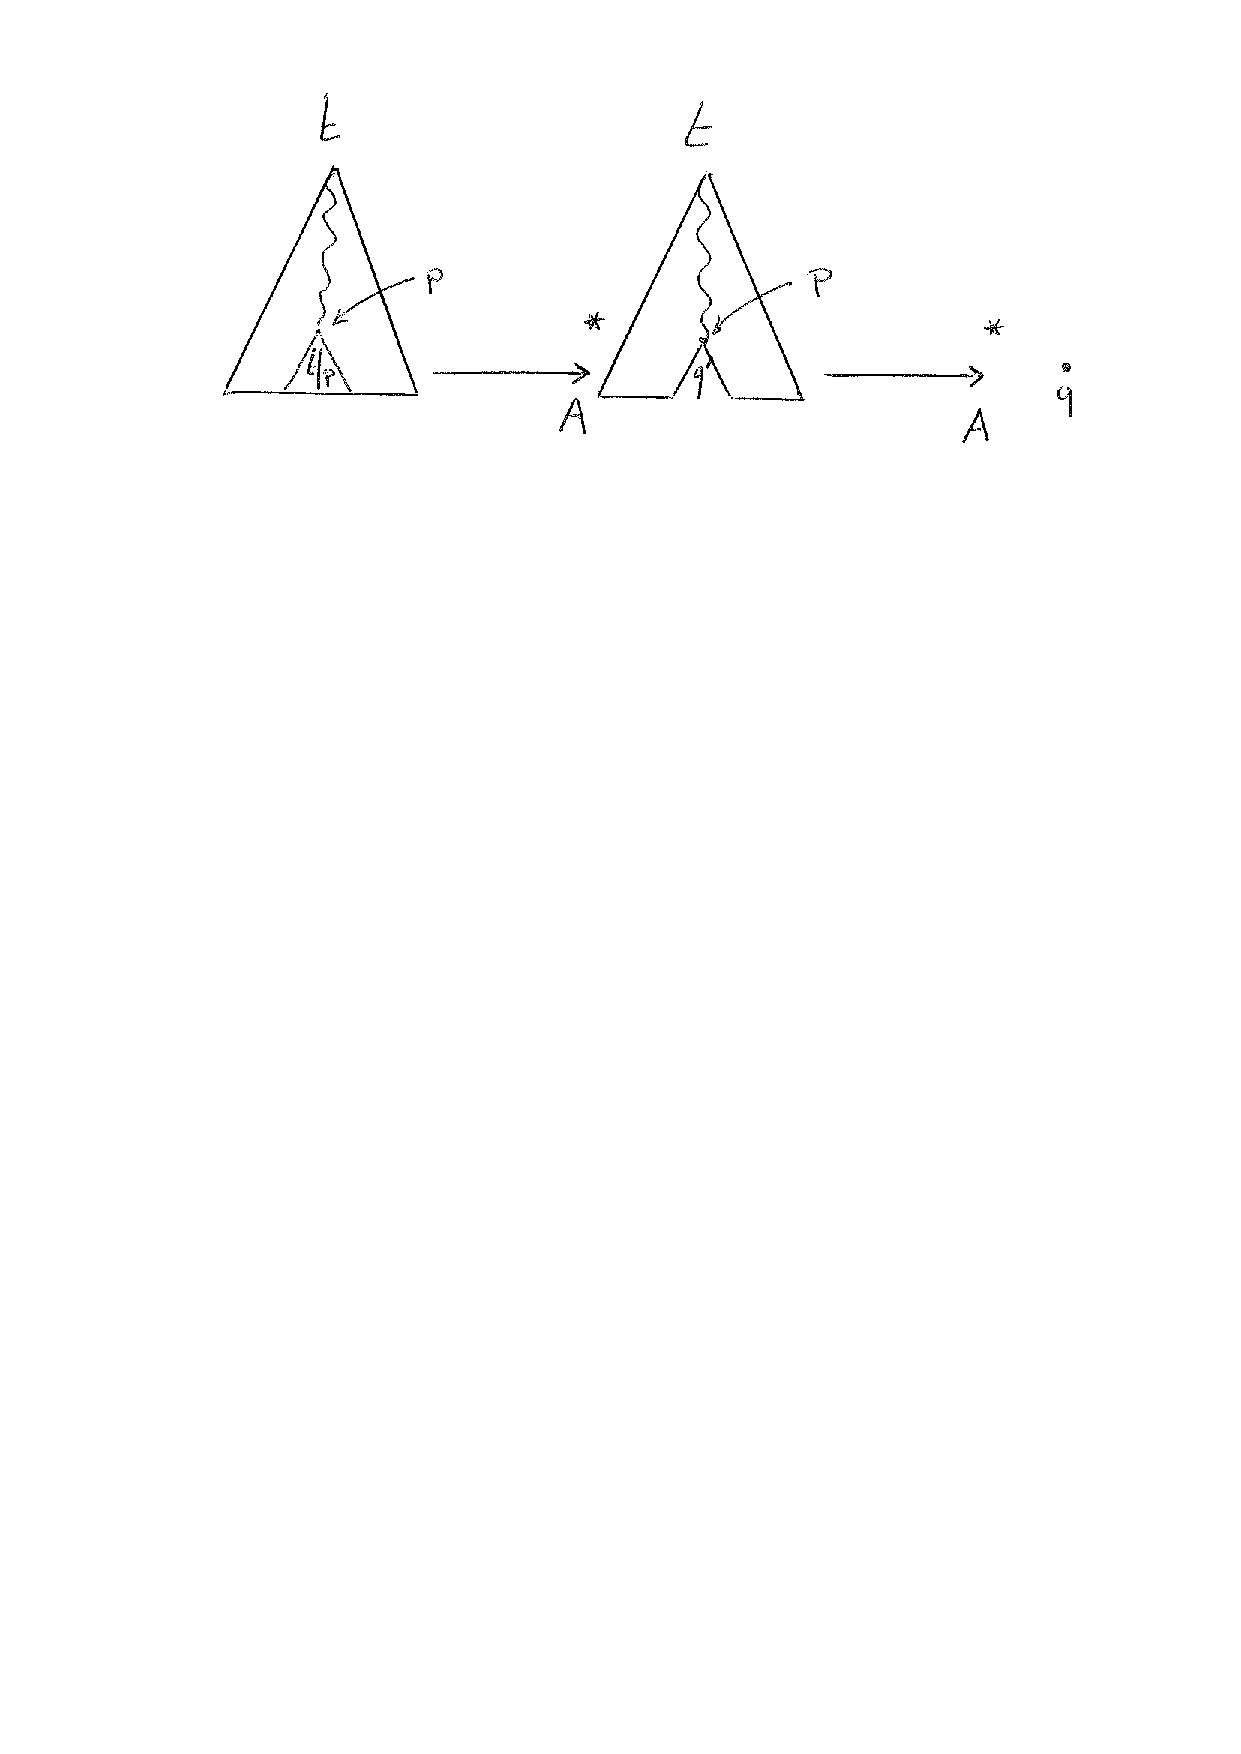
\includegraphics[width=12cm]{2_prerequis/automate_rev}
\end{property}


% \begin{corolary}
%   Soit une configuration $c \in \TFQ$. On définit l'ensemble des termes qui peuvent se réécire en $c$ par un automate $\A$
%   par un ensemble de substitutions de $\tau: \Q \f \TF$. Chacune des substitutions associe à chaque état $q$  un terme clos
%   $\tau(q) \in \Lang(q, \A)$ ou l'état $q$ si $\Lang(q, \A) = emptyset$,
%     Ainsi, le terme Chacune de ses fonctions
% \end{corolary}

Soit $L \subseteq \TF$ un ensemble de ensembles de termes clos. Le langage $L$ est régulier si et seulement si il existe
un automate d'arbres $\A$ tel que $L = \Lang(\A)$. Les langages réguliers de termes sont clos par union, intersection, et 
complémentation. Cependant, il est important de noter que la complémentation nécessite de déterminiser l'automate d'arbres
ce qui peut entraîner une complexité exponentielle.

\section{Le Model-Checking régulier}

Dans cette thèse, on s'intéresse à la vérification de propriétés de systèmes,
et en particulier aux systèmes pour lesquels l'ensemble des états accessibles
est infini mais peut-être modélisé de manière finie~\cite{WB98}. 
Il est à noter que l'approche envisagée fonctionne aussi 
dans le cas de systèmes à ensemble fini d'états.

Le premier problème est de fournir une représentation symbolique 
pour exprimer et manipuler des ensembles potentiellement infinis
d'états. C'est une question récurrente en vérification qui est malheureusement
indécidable, et pour laquelle il n'existe que des solutions partielles.
Ici, l'angle d'attaque retenu est celui de la vérification de modèles
à base de langage régulier de termes plus communément appelée {\em Tree Regular Model Checking
  (TRMC)}\,\cite{ALRd05}. Cette approche est une extension de l'approche qui fut initialement introduite
pour calculer l'ensemble des états atteignables en utilisant les langages réguliers de mots~\cite{BJNT00,BLW03}.


En TRMC, on modélise un système de transitions (tel qu'un programme ou un protocole) par un triplet $(\F, I, Rel)$,
avec
\begin{itemize}
\item
$\F$ une signature permettant de construire $\TF$ l'ensemble des termes représentants les différentes configurations ou états
du système;

\item
  $I \subseteq \TF$ un ensemble régulier de configurations donc représentable par un automate d'arbres $\A$, 
  \textit{i.e.} $\Lang(\A)=I$;

\item $Rel$ est une relation de transition représentée par un ensemble de règles de réécriture
  \footnote{\footnotesize A l'origine, $Rel$ est modélisée par un transducteur d'arbres.
    Mais comme les automates d'arbres peuvent être vus comme une classe particulière de 
    systèmes règles de réécriture, on choisit ici de généraliser}.
  On impose à $\R$ d'être linéaire à gauche.
\end{itemize}

\noindent
Dans ce contexte, un programme sera alors représenté par un triplet $(\F,\A,\R)$.
Ce type de modélisation est très expressif, d'une part parce que les systèmes de réécriture
linéaires à gauche sont Turing-complet~\cite{HUET-78}, et d'autre part parce qu'il est facile de 
modéliser les protocoles cryptographiques~\cite{GenetK-CADE00}, ainsi qu'un
important sous-ensemble du ByteCode Java~\cite{BoichutGJL-RTA07}.
On considère le problème d'atteignabilité pour ce modèle.

\begin{definition}[Problème d'atteignabilité]
\label{def:reachability}
Soit un programme $(\F,\A,\R)$ et un ensemble $Bad$ de termes correspondant à des états
interdits que le programme ne doit jamais atteindre.
Le problème d'atteignabilité consiste à vérifier qu'il n'existe 
aucun terme de $\desc(\Lang(\A))$ qui soit dans $Bad$.
\end{definition}

Le problème d'atteignabilité permet de vérifier des propriétés de sûreté
pour le système considéré. L'ensemble $Bad$ décrit des configurations invalides 
qui ne doivent pas être atteignables pour le système.

Dans le cas d'un protocole cryptographique, $Bad$ peut décrire des
configurations résultant d'une attaque du protocole. Ex: le message
chiffré est révélé en clair à un protagoniste externe à la
transaction\dots.

Pour les programmes Java, $Bad$ peut décrire des états où l'on
s'apprête à accéder à une zone mémoire non définie. Ex: pointeur null,\dots

\section{La complétion d'automates d'arbres}
\label{sec:completion}
Dans le cas des systèmes à espace d'états fini (et de taille
raisonnable), le calcul de l'ensemble des termes atteignables
($\desc(\Lang(\A))$) peut se réduire à une simple énumération des
termes que l'on peut atteindre à partir des termes de l'ensemble
initial.  Mais il n'est pas possible d'utiliser une telle
technique sur les systèmes à espace infini d'états (ou trop
important). En effet, lorsque $\R$ ne termine pas ou si 
$\Lang(\A)$ est infini, l'ensemble $\desc(\Lang(\A))$ est
alors infini et n'est généralement pas calculable~\cite{GilleronTison-FI95}.
Dans ces cas, il est nécessaire d'\textit{accélérer} l'exploration de
l'espace d'états afin d'atteindre notamment les termes situés à une
\textit{distance infinie} des termes initiaux, pour se ramener à un 
\textit{temps de calcul} raisonnable.
C'est dans ce contexte que se place la \textbf{complétion d'automates d'arbres}
décrite dans~\cite{Genet-RTA98,FeuilladeGVTT-JAR04}.
C'est un semi-algorithme qui calcule un automate d'arbres, \textit{i.e.} une représentation
régulière (et donc finie) des ensembles infinis, qui est en général
une sur-approximation de l'ensemble des termes atteignables.
Elle peut être utilisée pour résoudre certaines instances du problème d'atteignabilité:
la complétion d'automates d'arbres est facilement paramétrable afin de définir 
la sur-approximation souhaitée~\cite{Genet-RTA98,FeuilladeGVTT-JAR04,Takai-RTA04}
pour le problème considéré.

\subsection{Principe général}

En utilisant l'algorithme de complétion on peut construire un
automate d'arbres $\B$ dont le langage $\Lang(\B) \supseteq
\desc(\Lang(\A))$ contient au moins tous les termes atteignables.  Il
est alors suffisant de vérifier que l'automate $\B$ ne reconnaît pas
de termes de $Bad$ -- \textit{i.e.} $\Lang(\B)\cap Bad = \emptyset$ --
pour montrer que le système n'atteint jamais aucune des configurations
de $Bad$ soit $\desc(\Lang(\A))\cap Bad=\emptyset$.


% Expressivité des systèmes de réécriture :
% permettant de modéliser facilement des systèmes états/transitions,
% Outils pour assurer des vérifier des propriétés correction.
% Dans ce cadre, vérifier si un terme est atteignable ou non ?
% meme si le problème indécidable, la complétion 
% d'automates d'arbres contribue à la collection des outils capables
% de traiter le problèmes pour des ensembles de termes importants ou infinis.

% Le problème d'atteignabilité en général sous branche du  model checking (propriété de sûreté).
% transposé en réécriture et résolution du problème:
% vérifier si un terme considéré comme non-atteignable n'est effectivement pas atteignable.
% La notion d'atteignailité est toujours défini pour problème composé un ensemble initial $I$ et un système de 
% réécréture, donnés explicitement ou non.
% Discussion autour de l'exactidude du résultat de la complétion d'automates d'arbres???


% \comments{Calcul d'un ensemble régulier des termes atteignables par réécriture. 
% Cet ensemble est une surapproximation régulière (parfois exacte) de  $\R^*(I)$.

% Principe est d'utiliser les automates d'arbres comme représentation des ensembles de termes.
% Puis de réécrire des configurations de l'automate. 
% Puisqu'une configuration représente un ensemble de termes, réécriture d'une configuration de l'automate
% $\equiv$ réécrire un ensemble de termes.
% }

La complétion d'automates d'arbres termine lorsque le calcule arrive sur un point fixe,
lorsque l'automate est $\R$-clos.


\begin{definition}
  Un automate d'arbres $\B$ est dit $\R$-clos si chaque état $q$ de cet automate et pour tous termes $s,t$ tels que 
  $s \rw_\R t$ avec $s$ reconnu par $\B$ dans l'état $q$, alors $t$ est aussi reconnu par $\B$ dans l'état $q$.
  La propriété de clôture est illustrée par le diagramme de la figure~\ref{fig:R-cloture}.
  % The situation is represented with the following graph.
  \begin{figure}[ht!]
    \centering
    $
    \xymatrix{
      s \ar[r]_{\R}\ar[d]^{*}_{\B} & t \ar@/^1.2pc/[ld]_{*}^{\B}\\
      q & %\ar[l]^{\A_{i+1}} q'
    }
    $
    \caption{\footnotesize Propriété de $\R$-clôture}
    \label{fig:R-cloture}
  \end{figure}
\end{definition}

Il est évident de constater que l'on a $\Lang(\B) \supseteq \desc(\Lang(\A))$
si $\B$ est $\R$-clos et si $\Lang(\B)\supseteq \Lang(\A)$~\cite{BoyerGJ-IJCAR08}.

D'un point de vue algorithmique, la construction d'un automate $\R$-clos, que l'on notera
$\aaex^*$, à partir de l'automate $\A$ consiste à \textit{compléter} l'automate $\A$
par de nouvelles transitions pour étendre son langage. L'algorithme de complétion
calcule une succession d'automates $\aaex^1,\aaex^2,\ldots$ en appliquant à chaque fois
l'ensemble des règles de réécriture sur $\aaex^i$ pour produire $\aaex^{i+1}$.
Le calcul peut s'arrêter lorsque l'on obtient un automate $\R$-clos 
$\aaex^k$ \textit{i.e.} tel que $\Lang(\aaex^{k+1}) \supseteq \Lang(\aaex^k)$.

\subsection{Étape de complétion : calcul exact des $\R$-descendants}


Chaque application du TRS $\R$ est appelée \textbf{étape de complétion} et 
consiste à rechercher parmi les termes reconnus par l'automate, ceux qui peuvent être réécrits
dont les descendants ne sont pas encore reconnus par l'automate.
Cela revient à rechercher les \textbf{paires critiques} $\langle q, t \rangle$ 
pour lesquelles le diagramme de la figure~\ref{fig:R-cloture} n'est pas clos, \textit{i.e.}
on a $s \rw_\R t$ et $s \rw_{\A}^* q$ mais pas $t \not\rw_{\A}^* q$.

On ne considère que les paires critiques dont l'origine est localisée à la racine du terme c'est à dire
que la position $p$ à laquelle le terme est réécrit par $\R$ est $p = \epsilon$.
En effet, quelle que soit la position $p \in \pos(s)$ à laquelle on décide de réécrire le terme
$s$, on peut toujours revenir au cas d'une paire critique où la réécriture n'a lieu qu'à la racine du terme.
Il suffit de considérer l'exécution $s \rw_\A^* q$ par l'automate $\A$. 
On sait que le terme $s$ se réécrit à la position $p \in \pos(s)$ par une règle $l \rw r$ de $\R$. Ce qui signifie que le sous-terme à la 
position $p$ est une instance de $l$ donc de la forme $l\tau$, où $\tau$ est une substitution $\X \f \TF$.
Or d'après la propriété~\ref{prop:execution}, comme $s$ est reconnu par l'automate $\A$, c'est aussi le cas pour chacun de ses sous-termes
et donc en particulier il existe un état $q'$ tel que $l\tau \rw_\A^* q'$. On peut donc simplifier le problème de la paire critique $\la q, t\ra$ à la position $p$
en considérant la paire critique $\la q', r\tau\ra$ à la position $\epsilon$.


\begin{figure}[ht!]
  \centering
  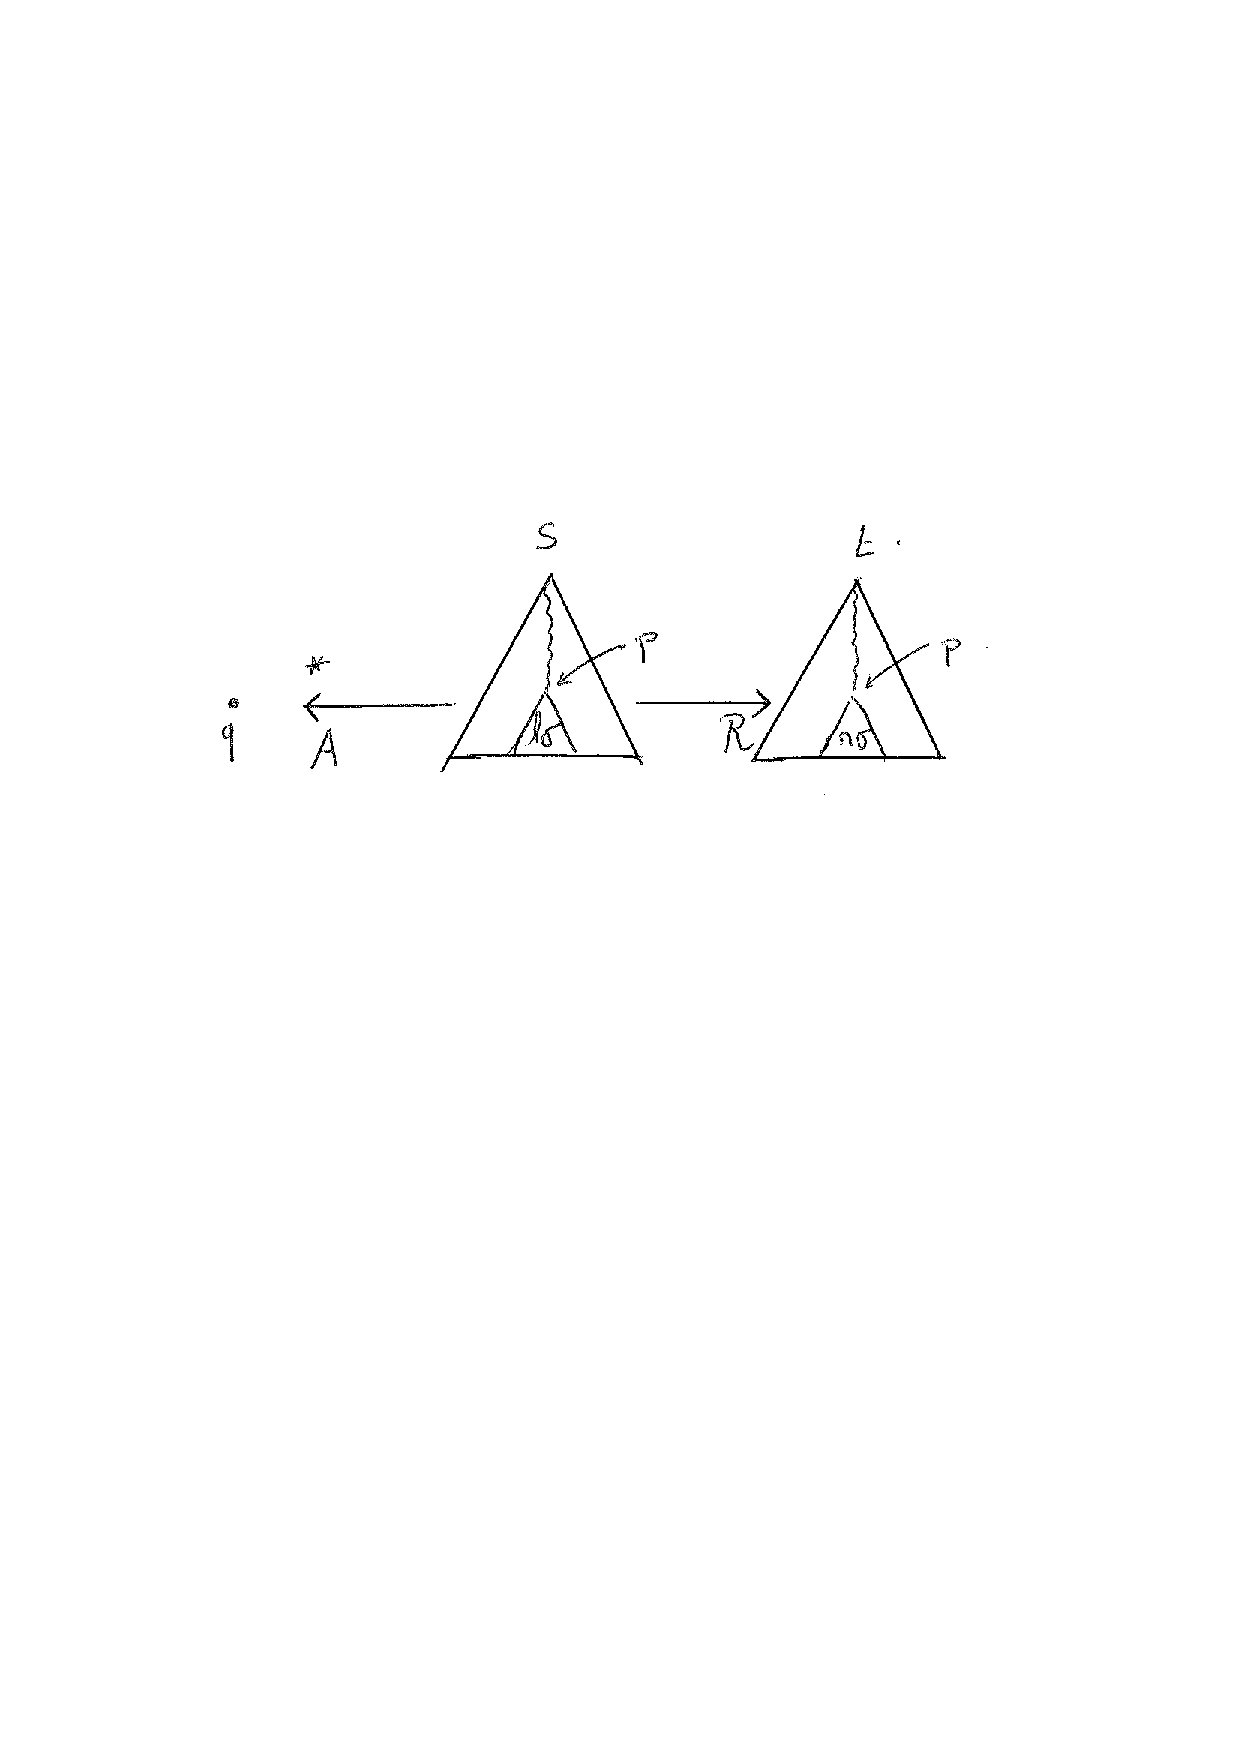
\includegraphics[width=12cm]{2_prerequis/cp1}
\end{figure}
% \comments{FIGURE PAIRES CRITIQUES 1}
Ce qui revient à\\
\begin{figure}[ht!]
  \centering
  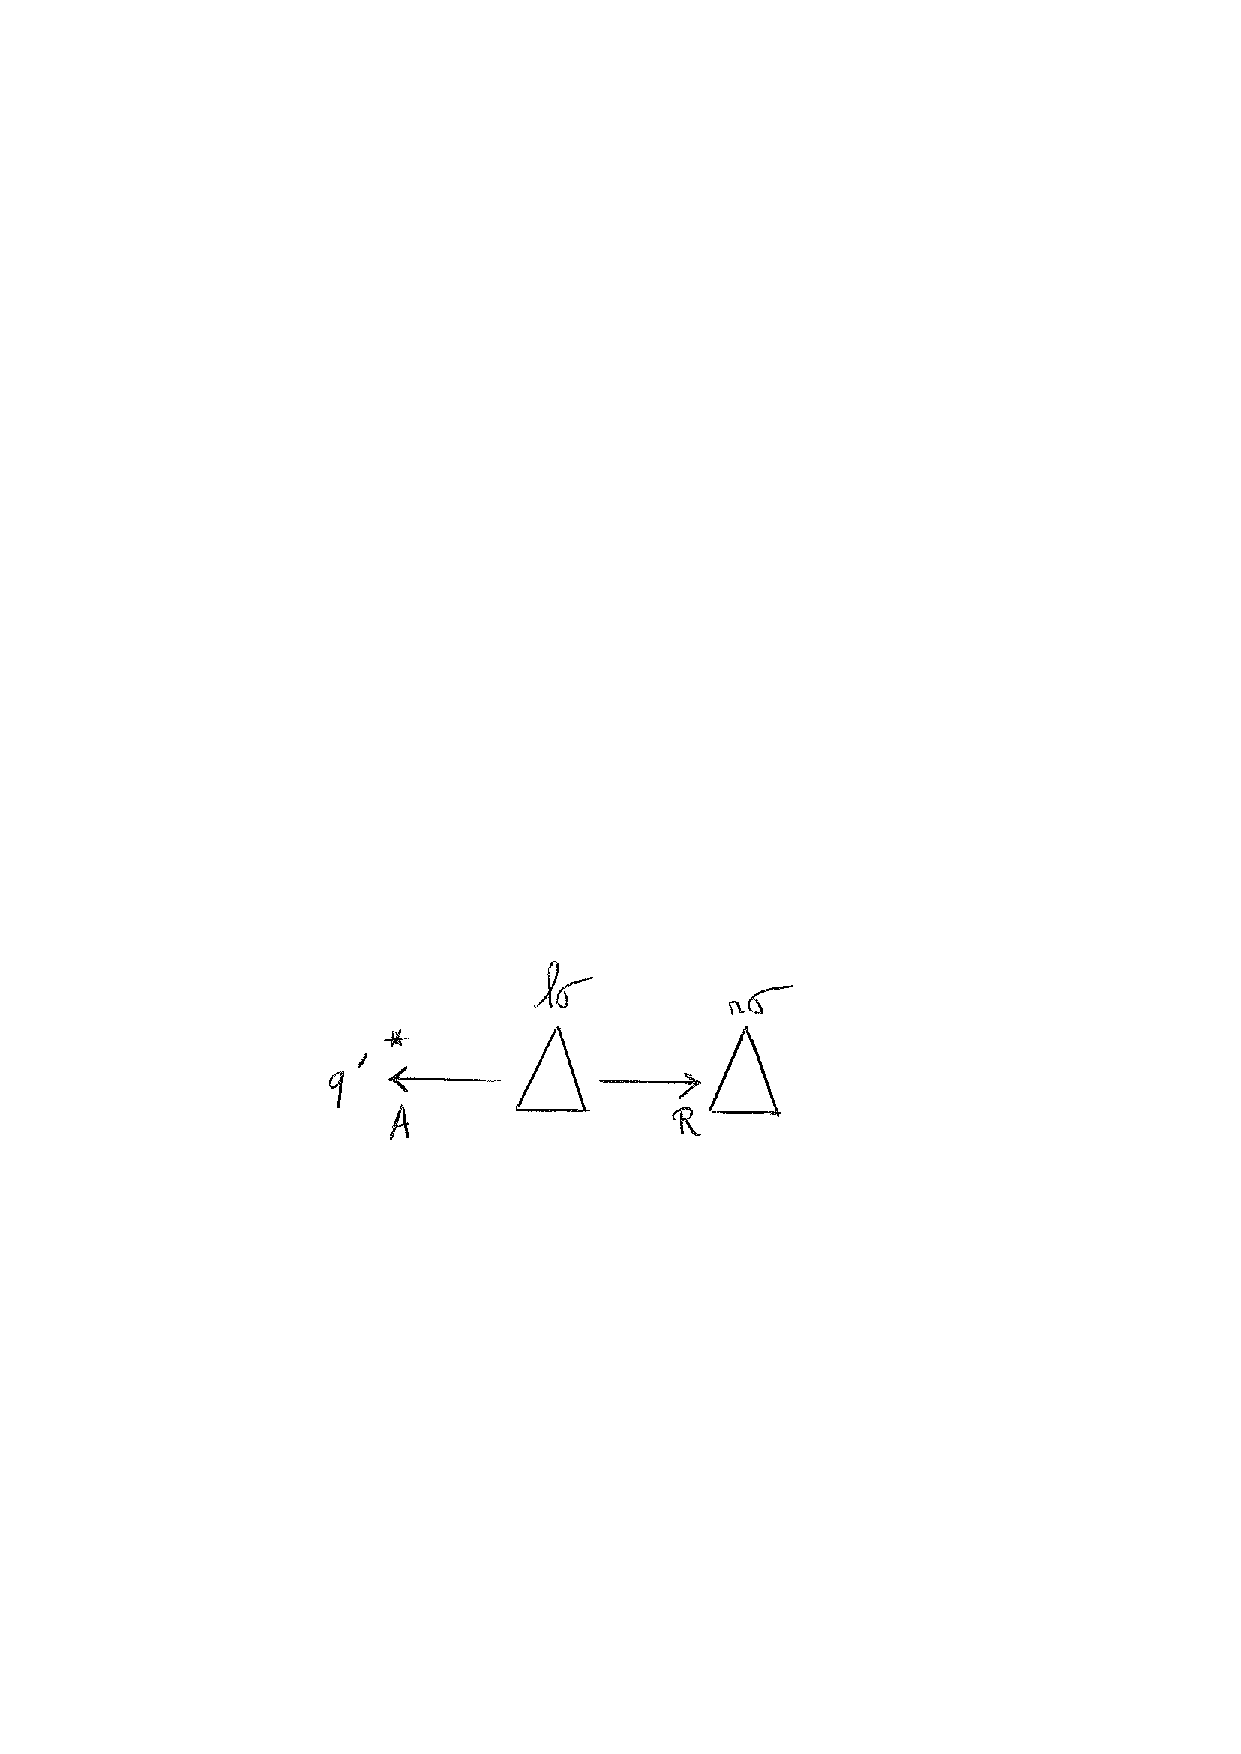
\includegraphics[width=8cm]{2_prerequis/cp2}
\end{figure}

%\comments{FIGURE PAIRES CRITIQUES 2}

% remis car il faut introduire la notation \aaex^i, utilisée dans la suite.
Une étape de complétion résout toutes les paires critiques en construisant
à partir de l'automate $\A$, un nouvel automate $\aaex^1$ avec des transitions
supplémentaires de façon à obtenir $t \rw_{\aaex^1}^* q$. Cela correspond
au résultat de l'application $\R$ sur le terme $s$. Ensuite on réapplique la procédure
pour résoudre les paires critiques de $\aaex^1$ pour construire $\aaex^2$ jusqu'à obtenir
un automate $\aaex^*$ qui soit exempt de paires critiques. En construisant l'automate $\aaex^*$,
on a atteint un point fixe, et $\aaex^*$ est $\R$-clos.

Comme le langage reconnu par l'automate $\aaex^i$ peut-être infini, l'ensemble
des paires critiques $\la q, r\tau\ra$ pour la règle $l\rw r\in \R$ peut lui aussi être infini : 
l'ensemble des termes $l\tau$ reconnus dans l'état $q$ peut-être infini. Chacun des termes $l\tau$
pouvant se réécrire en $r\tau$, on a bien une infinité de paires critiques, qu'il n'est pas envisageable
d'énumérer.
La solution retenue dans~\cite{Genet-RTA98} pour contourner ce problème consiste à construire des ensembles de
substitutions $\sigma: \X \mapsto \Q$ -- appelées $\Q$-substitutions -- associant à chaque variable des règles de réécriture 
un état de l'automate. L'ensemble de substitutions à considérer est fini. En effet le domaine des substitutions est restreint à l'ensemble des
variables apparaissant dans les règles de réécriture, qui est un ensemble fini. De même, l'ensemble $\Q$ des états de l'automate est fini.
Cependant, un état peut reconnaître un ensemble infini de termes, et donc l'instance $l\sigma$ peut représenter une infinité de termes.
On peut construire l'ensemble des termes dénotés par $l\sigma$ par un ensemble de substitutions $\eta: \Q \f \TF$ qui associe à chaque état $q$ 
un terme $\eta(q)$ reconnu par l'automate $\A$ en l'état $q$. % (on sait que $\Lang(\A, q) \not= \emptyset$).
Ce qui donne 
\[\forall \eta \in \{ \eta : \Q \rw \TF \sep \eta(q) \rw_\A^* q\},\quad l\sigma.\eta \rw^*_\A  l\sigma\]
Ainsi, réécrire $l\sigma$ en $r\sigma$ revient donc à réécrire tous les termes $l\sigma.\eta$ en $r\sigma.\eta$ du point de vue de l'automate.

\paragraph{Recherche des paires critiques}
\label{sec:recherche-des-paires}

\begin{definition}
  Pour $\aaex^i$ un automate d'arbres donné et $l \rw r \in \R$ une
  règle de réécriture, on appelle le \textbf{problème de filtrage}, le
  problème qui consiste à retrouver toutes les paires critiques de $l
  \rw r$ avec $\aaex^i$. On utilise $l \match q$ pour dénoter plus précisément
  le problème de filtrage pour tout état $q$ de $\aaex^i$.
\end{definition}

La complétion utilise un \textbf{algorithme de filtrage}~\cite{FeuilladeGVTT-JAR04}
pour résoudre chaque problème $l \match q$ dans l'automate $\aaex^i$. 
Cet algorithme produit un ensemble de $\Q$-substitutions $\sigma: \X \mapsto \Q$
formant des paires critiques $\la q, r\sigma\ra$ telles que $l\sigma \rw_{\aaex^i}^* q$.
Le problème de filtrage doit être résolu pour toutes les règles $l\rw r$ de $\R$ avec
chaque état $q$ de l'automate $\aaex^i$.

\begin{definition}
  Une paire critique $\la q, r\sigma\ra$ est non résolue entre l'automate $\aaex^i$ et $\R$ si $r\sigma \not\rw_{\aaex^i}^* q$.
  \begin{figure}[ht!]
    \centering
    $
    \xymatrix{
      l\sigma \ar[r]_{\R}\ar[d]^{*}_{\aaex^i} & r\sigma \\%\ar@/^1.2pc/[ld]_{*}^{\aaex^{i+1}}\\
      q & %\ar[l]^{\A_{i+1}} q'
    }
    $
    \caption{\footnotesize Paire critique non résolue\label{fig:cp}}
  \end{figure}  
\end{definition}

\paragraph{La résolution des paires critiques} consiste simplement à ajouter la nouvelle transition $r\sigma \rw q$.
Il y a deux variantes pour ajouter cette transition. L'ajout immédiat de la transition $r\sigma \rw q$
ou l'ajout des transitions $r\sigma \rw q'$ et $q' \rw q$. La deuxième version plus récente, permet de 
gagner en information: la transition $q' \rw q$ permet de distinguer les termes reconnus en $q'$, comme 
un sous-ensemble des termes $q$, conséquence de l'étape de complétion. Sans l'utilisation de la $\varepsilon$-transition,
il n'est pas possible à posteriori de distinguer les successeurs $r\sigma$. 
Dans la suite, on ne considère plus que la variante $r\sigma \rw q'$ et $q' \rw q$ pour résoudre les paires critiques,
sauf au chapitre~\ref{chap:certif} où l'on considère un automate  sans $\varepsilon$-transitions
qu'il est toujours possible d'obtenir par nettoyage des $\varepsilon$-transitions.

En général, les transitions $r\sigma \rw q'$ ne respectent pas la définition~\ref{def:transitions}
et doivent être normalisées avant d'être ajoutées à l'automate.


%\comments{definition de la normalisation}
\begin{definition}
  La \textbf{normalisation} d'une transition $r\sigma \rw q'$ transforme cette
  transition en un ensemble $\Pi$ de transitions normalisées~\ref{def:transitions}
  telles que $r\sigma \rw_\Pi^* q'$. Les transitions sont ensuite ajoutées aux transitions de $\aaex^i$.
\end{definition}
On notera que la définition normalisation~\cite{Genet-RTA98} nécessite 
souvent l'utilisation de nouveaux états dans l'automate pour construire 
les nouvelles transitions. C'est d'ailleurs le critère le plus important
à considérer du point de vue de la terminaison. Il est important de limiter le
plus possible la création de nouveaux états, pour limiter la divergence.

\begin{definition}
  On note $\compl(\aaex^i)$, l'\textbf{étape de complétion} qui consiste à rechercher les paires critiques présentes
  dans $\aaex^i$ pour les résoudre dans l'automate $\aaex^{i+1} = \compl(\aaex^i)$.
\end{definition}

\begin{property}
  Soient $\aaex^i$ un automate, et $\aaex^{i+1} = \compl(\aaex^i)$ l'automate obtenu après une
  étape de complétion par $\R$, alors
  \begin{itemize}
  \item $\Lang(\aaex^i) \subseteq \Lang(\aaex^{i+1})$

  \item  pour tous termes $s \in \Lang(\aaex^i)$ et $t \in \TF$,
    \[s \rw_\R t \imp t\in \Lang(\aaex^{i+1})\]
  \end{itemize}
\end{property}


\paragraph{Sémantique liée aux $\varepsilon$-transitions}
Lors de la résolution d'une paire critique, la transition $r\sigma \rw q'$ reliée à l'état $q$ par le biais de la transition
$q' \rw q$. Cette $\varepsilon$-transition permet de créer une relation d'ordre entre les termes dans l'automate.
En effet, si l'on se place du point de vue de l'état $q$, on a bien étendu le langage en lui ajoutant $r\sigma.\eta$
les termes représentés par la configuration $r\sigma$. Or si l'on se place du point de vue de l'état $q'$, on ne verra dans $\Lang(\A,q')$
que les termes $r\sigma.\eta$ et leurs $\R$-descendants. Donc à moins que certains des termes déjà présents avant la résolution
de la paire critique $\la q, r\sigma\ra$ ne soient des $\R$-descendants de termes reconnus par $q'$, ils ne seront pas dans $\Lang(\A, q')$.
En fait, il est possible de définir plus formellement cette relation d'ordre.
\begin{definition}
  \label{def:representants}
  Soit $\A$ un automate d'arbres. On définit par $\rwne_\A$ la relation induite par les transitions normalisées de $\A$.
  On appelle \textbf{représentants} de l'état $q$, tous les termes clos de l'ensemble $\Rep(q) = \{t \in \Lang(\A, q)\sep t \rwne_\A q\}$.
\end{definition}

Par définition l'automate $\aaex^0 = \A$ représente l'ensemble initial et n'a jamais été complété : on impose alors qu'il ne contienne pas 
de $\varepsilon$-transitions. Seule la résolution des paires critiques ajoute des $\varepsilon$-transitions à l'automate.
La complétion d'un automate d'arbres par $\R$ assure alors la propriété suivante:


\begin{property}
  Soit l'automate $\aaex^i$ obtenu par complétion. Pour tout état $q$, 
  chaque terme reconnu en l'état $q$ est le successeur par réécriture d'un représentant 
  de l'état $q$:
  \[\forall t \in \Lang(\aaex^i, q), \exists s \in Rep(q) \st s \rw_\R^* t\]
\end{property}



\paragraph{Vers une approximation de $\desc(\Lang(\A))$}


Cependant, excepté pour des classes particulières de TRS~\cite{FeuilladeGVTT-JAR04,Genet-Habil},
l'automate représentant l'ensemble des termes atteignables ne peut pas être obtenu
à partir de $\A$ en appliquant un nombre fini de fois l'étape de complétion\dots


\begin{example}
  Soit $\R = \{0 \rw S(0),\ S(x) \rw S(S(x))\}$ qui engendre l'ensemble des entiers naturel
  à partir de l'automate $\A_0$ consitué de l'unique transition $0 \rw q_0$ avec l'état $q_0$ final.
  Le tableau suivant résume quelles paires critiques sont résolues et les transitions ajoutées par chaque étape de complétion
  pour obtenir l'automate $\A_i$:
  \begin{center}
    \begin{tabular}{|cll||l|}
      \hline
      $\A_0$ : & $0 \rw q_0$ & - & - \\
      \hline
      $\A_1$ : & $S (q_0) \rw q_1$ & $q_1 \rw q_0$ & $\la q_0, S(0)\ra$\\
      \hline
      $\A_2$ : & $S (q_1) \rw q_2$ & $q_2 \rw q_1$ & $\la q_1, S(S(q_0))\ra$\\
      \hline
      $\A_3$ : & $S (q_2) \rw q_3$ & $q_3 \rw q_2$ & $\la q_2, S(S(q_1))\ra$\\
      \hline
      $\A_4$ : & $S (q_3) \rw q_4$ & $q_4 \rw q_3$ & $\la q_3, S(S(q_2))\ra$\\
      & \vdots & \vdots & \vdots \\
      & \vdots & \vdots & \vdots \\
      \hline
    \end{tabular}
  \end{center}

  On peut voir que le calcul diverge, car le nouvel état introduit
  à chaque étape de complétion, fournit une nouvelle paire critique avec la règle $S(x) \rw S(S(x))$.

  On peut aussi remarquer qu'une fois que la paire critique est résolue en l'état $q_i$,
  elle est aussi résolue pour tous les états $q'$ qui sont accessibles par des $\varepsilon$-transitions.
  Lorsque l'on a $l\sigma \rw^*_{\A_i} q_i$ et $r\sigma \rw^*_{\A_i} q_i$ alors pour tout état $q$ tel
  que $q_i \rw^*_{\A_i} q$,la paire critique $\la q, r\sigma\ra$ est aussi résolue. On utilise cette
  propriété pour optimiser la recherche des paires critiques.
\end{example}


Le processus de complétion requiert alors une accélération pour terminer. Pour cela on peut
utiliser une technique d'approximation basée sur un ensemble d'équations $E$ et produire 
une sur-approximation de l'ensemble des termes atteignables, \textit{i.e.} un automate d'arbres
$\aapprox$ tels que $\Lang(\aapprox) \supseteq \desc(\Lang(\A))$.

L'accélération consiste à définir un nouvel automate $\aaexeq^i$ à partir de l'automate $\aaex^i$ tel 
que le langage de $\aaexeq^i$ soit une sur-approximation du langage de $\aaex^i$.
L'approximation repose sur la relation $=_E$ induite par les équations $E$. 
Elle consiste à fusionner les états dont les représentants (\textit{c.f.} définition~\ref{def:representants})
dans la même classe d'équivalence par $=_E$. La fusion correspond au un renommage des états destinés à la fusion
par un nouveau nom d'état. Cette étape de renommage est réalisée pour l'intégralité des transitions de l'automate.
%Elle repose sur la \textbf{fusion d'états} dirigée par les équations de $E$.
\begin{definition}
  Deux états distincts $q,\ q'$ de l'automate $\aaex^i$ sont \textbf{fusionnés} si pour une équation $u=v \in E$,
  il existe une $\Q$-substitution $\sigma : \X \rw \Q$ telle qu'on ait le diagramme de la figure~\ref{fig:fusion}.

  \begin{figure}[ht!]
    \centering
    $\xymatrix{
      u\sigma \ar@{=}[r]_{E}\ar[d]_{\aaex^i}^{\not\varepsilon} & v\sigma \ar[d]_{\not\varepsilon}^{\aaex^i}\\
      q & q'
    } $
    \caption{Fusion d'états par l'équation $u=v$}
    \label{fig:fusion}
  \end{figure}

  Alors on fusionne les états $q$ et $q'$ dans l'automate $\aaexeq^i$. 
  La fusion consiste alors en un simple renommage de $q$ en $q'$ (ou inversement) dans toutes
  les transitions de l'automate où l'état $q$ apparaît.
  % Les ensembles des substitutions $\sigma$ et $sigma'$
  % peuvent être calculées respectivement par résolution des problèmes de filtrage $u \match q$ et $v \match q'$.
  % Il suffit de vérifier si il existe un couple $(\sigma,\sigma')$ tel que pour toute variable $x \in \vars(u) \cap \vars(v)$
  % $\sigma(x) = \sigma(x')$. 
\end{definition}


\begin{definition}
  On définit $\widen$, la fonction d'accélération paramétrée par $E$ un ensemble d'équations, 
  que l'on applique après chaque étape de complétion sur l'automate $\aaex^i$. Elle construit
  un nouvel automate $\aaexeq^i = \widen(\aaex^i)$, en fusionnant tous les couples d'états de $\aaex^i$
  qui peuvent l'être.
\end{definition}


\begin{example}
  On reprend l'exemple précédent qui diverge, et on tente d'appliquer l'équation $x = S(S(x))$ sur
  l'automate $\A_2$ (il n'est en fait pas possible de l'appliquer plus tôt).
  L'automate $\A_2$ est composé des transitions $\{ 0 \rw q_0,\ S(q_0) \rw q_1,\ S(q_1) \rw q_2\}$
  et $\{ q_2 \rw q_1,\ q_1 \rw q_0\}$.
  On trouve alors la substitution $x \mapsto q_0$, ce qui donne $q_0 = S(S(q_0))$ et $S(S(q_0)) \rw^*_{\A_2} q_2$.
  On fusionne donc les états $q_2$ et $q_0$, et obtient le nouvel automate $\A_2'$ dans lequel on remplace
  $q_2$ par $q_0$, ce dont on déduit les transitions $\{ 0 \rw q_0,\ S(q_0) \rw q_1,\ S(q_1) \rw q_0\}$
  et $\{ q_0 \rw q_1,\ q_1 \rw q_0\}$.
  
  On cherche les nouvelles paires critiques en $q_0$ et $q_1$ pour les règles de $\R = \{0 \rw S(0),\ S(x) \rw S(S(x))\}$.
  On trouve $\la q_0, S(0)\ra$ qui est déjà résolue, puis les paires $\la q_0,S(S(q_0))\ra$ et $\la q_1,S(S(q_1))\ra$
  qui sont aussi résolues: l'automate $\A_2'$ est clos par $\R$, on a atteint un point fixe.
\end{example}


On relie alors les étapes de complétion et d'accélération en posant $\aaexeq^0=\A$, puis en combinant
complétion et accélération $\aaexeq^{i+1}= \widen(\compl(\aaexeq^i))$, jusqu'à l'obtention d'un point fixe
$\aapprox$, automate $\R$-clos.

Dans ~\cite{GenetR-JSC10}, il a été montré que si l'automate initial respecte la $\RE$-cohérence,
$\aapprox$ est un automate $\RE$-cohérent qui ne reconnaît pas plus de termes que les termes atteignables
par réécriture de $\R$ modulo $E$.
\begin{definition}
  \label{def:re-coherence}
  Un automate $\A$ est $\RE$-cohérent~\cite{GenetR-JSC10} si et seulement si pour tout état $q$, il existe 
  $s \in \Rep(q)$ un représentant de l'état $q$ tel que~:
  \begin{itemize}
  \item $\forall t \in \Rep(q)$, $s =_E t$
  \item $\forall t \in \Lang(\A, q)$, $s \rw_\RE^* t$.
  \end{itemize}
\end{definition}

Cette technique d'approximation et cette méthodologie sont comparables à celle employée 
par les abstractions équationnelles définies dans~\cite{MeseguerPM-TCS08}.

% If the intersection between $\aapprox$ and $Bad$ is not empty, then it
% does not necessarily mean that the system does not satisfy the
% property. There is thus the need for techniques to decide whether a
% counter-example is indeed a reachable term that does not satisfy the
% property or if it is a term added by the abstraction and that cannot
% be reached from the set of initial states. If the latter case occurs,
% one has to propose a refinement technique that will remove the
% false-positive from the abstraction. Studying such techniques for
% completion automata is the main objective of this paper.

%%The rest of the paper is organized as follows. In Section
%%\ref{sec:re-automaton}, we introduce $\RE$-automaton that is an
%%extended tree automata. Section \ref{sec:re-automaton} proposes a
%%completion algorithm for $\RE$-automata, while Section \ref{} shows
%%how the extended structure can be used to refine in an efficient
%%manner.




% Tree automata completion~\cite{genet-RTA98,FeuilladeGVTT-JAR04,GenetR-JSC10} is
% an algorithm for computing sets of reachable terms $\desc(I)$, given a regular
% language of initial terms $I=\Lang(\A)$. For most of the known classes of TRS
% $\R$ for which $\desc(\Lang(\A))$ is regular, the output of completion is a tree automaton
% $\aaex^*$ such that $\Lang(\aaex^*)=\desc(\Lang(\A))$. When
% $\desc(\Lang(\A))$ is not regular, it is possible to parameterize the algorithm
% by a set of equations $E$, and to compute a tree automaton $\aapprox$ 
% over-approximating reachable terms,
% i.e. $\Lang(\aapprox) \supseteq \desc(\Lang(\A))$. 



%\subsection{B}


% \begin{figure}[!ht]
% \hfill
% \begin{tabular}[b]{lll}
% \begin{minipage}{3cm}
% {\small
% $
% \xymatrix{
%   l\sigma \ar[r]_{\R}\ar[d]^{*}_{\aaex^i} & r\sigma \ar@/^1.2pc/[ld]_{*}^{\aaex^{i+1}}\\
%   q & %\ar[l]^{\A_{i+1}} q'
% }
% $}
% \caption{Critical pair\label{fig:cp}}
% \end{minipage} & \hspace*{2cm} &
% \begin{minipage}{4cm}
% {\small
% $\xymatrix{
% u\sigma \ar@{=}[r]_{\E}\ar[d]_{\aaex^{i+1}}^{*} & v\sigma \ar[d]_{*}^{\aaex^{i+1}}\\
% q & q'
% }
% $}
% \caption{Detection of merging \label{fig:merge}}
% \end{minipage}
% \end{tabular}
% \hfill ~
% \end{figure}

%\vspace*{-10mm}
% \begin{figure}[!ht]
% \hfill
% \begin{minipage}{3cm}
% {\small
% $
% \xymatrix{
%   l\sigma \ar[r]_{\R}\ar[d]^{*}_{\aaex^i} & r\sigma \ar@/^1.2pc/[ld]_{*}^{\aaex^{i+1}}\\
%   q & %\ar[l]^{\A_{i+1}} q'
% }
% $}
% \caption{Critical pair\label{fig:cp}}
% \end{minipage}
% \hfill
% \begin{minipage}{4cm}

% %\vspace{3mm}
% {\small
% $\xymatrix{
% u\sigma \ar@{=}[r]_{\E}\ar[d]_{\aaex^{i+1}}^{*} & v\sigma \ar[d]_{*}^{\aaex^{i+1}}\\
% q & q'
% }
% $}
% \caption{Detection of merging \label{fig:merge}}
% \end{minipage}
% \hfill ~
% \end{figure}

% %\vspace*{-8mm}
% However, the transition $r \sigma \f q$ is not necessarily a normalized
% transition of the form $f(q_1, \ldots, q_n) \f q$ and so it has to be normalized
% first. Thus, instead of adding $r\sigma \rw q$ we add $\norm(r\sigma \rw q)$ to
% transitions of $\aaex^i$.
% Here is the $\norm$ function used to normalize transitions. Note that, in 
% this function, transitions are normalized using either new states of $\Q_{new}$
% or states of $\Q$, states of the automaton being completed. As we will see in
% Lemma~\ref{lemma:approx}, this has no effect on the safety of the normalization
% but only on its precision.

%  \begin{definition} [$\norm$] Let $\A=\aut$ be a tree automaton, $\Q_{new}$ a
%    set of {\em new} states such that $\Q\cap \Q_{new} = \emptyset$, $t \in \TFQ$ and $q\in
%    \Q$.  The function $\norm$ is inductively defined by:
%   \begin{itemize}
%     \item 
%     $\norm(t \rw q)= \emptyset$ if $t=q$,
%     \item 
%     $\norm(t \rw q)= \{c \rw q \sep c\rw t \in \Delta\}$ if $t \in \Q$,
%     \item 
%     $\norm(f(t_1, \ldots, t_n) \rw q)= \bigcup_{i =1 \ldots n} \norm(t_i \rw
%     q_i) \cup \{f(q_1, \ldots, q_n) \rw q\}$ where $\forall i=1\ldots n: (t_i
%     \in \Q \Rightarrow q_i=t_i) \wedge (t_i \in \TFQ\setminus \Q \Rightarrow q_i \in \Q\cup \Q_{new})$.
%   \end{itemize}
% \end{definition}

% When using only new states to normalize all the new transitions occurring in all
% the completion steps, completion is as precise as possible.  However, doing so,
% completion is likely not to terminate (because of general undecidability
% results~\cite{GilleronTison-FI95}).  Enforcing termination of completion can be
% easily done by bounding the set of new states to be used with $\norm$ during the
% whole completion. We then obtain a finite tree automaton over-approximating the
% set of reachable states. The fact that normalizing with any set of states (new
% or not) is {\em safe} is guaranteed by the following simple lemma. For the
% general safety theorem of completion see~\cite{FeuilladeGVTT-JAR04}.

% \begin{lemma}
% \label{lemma:approx}
% For all tree automaton $\A=\aut$, $t\in \TFQ\setminus \Q$ and $q\in\Q$, if $\Pi=\norm(t \rw
% q)$ whatever the states chosen in $\norm(t \rw q)$ we have $t \rw^*_{\Pi} q$.
% \end{lemma}
% \begin{proof}
% This can be done by a simple induction on transitions~\cite{FeuilladeGVTT-JAR04}.
% %to normalize, see~\cite{FeuilladeGVTT-JAR04}.
% \end{proof}

% To let the user of completion guide the approximation, we use two different
% tools: a set $\nr$ of {\em normalization rules} (see~\cite{FeuilladeGVTT-JAR04})
% and a set $\E$ of {\em approximation equations}. Rules and equations can be
% either defined by hand so as to prove a complex
% property~\cite{GenetTTVTT-wits03}, or generated automatically when the property
% is more standard~\cite{BoichutHKO-AVIS04}. Normalization rules can be seen as a
% specific strategy for normalizing new transitions using the $\norm$
% function. We have seen that Lemma~\ref{lemma:approx} is enough to
% guarantee that the chosen normalization strategy has no impact on the safety of
% completion. Similarly, for our checker, we will see in Section~\ref{sec:closure}
% that the related \coq\ safety proof can be carried out independently of the
% normalization strategy (i.e. set $N$ of normalization rules).  On the opposite, the
% effect of approximation equations is more complex and has to be studied more
% carefully.
% % On the one side, normalization
% % rules define which states are to be used to normalize a transition with
% % $\norm$. When using $\nr$ to guide the normalization, we note $\norm_{\nr}$ the
% % normalization function.  On the other side, approximation equations define some
% % approximated equivalence classes. Equations of $\E$ are applied directly on
% % $\A^{i+1}_{\R}$ to merge together the states whose recognized terms are in the
% % same equivalence class w.r.t. $\E$.
% %
% % For all $s,l_1, \ldots, l_n \in\TFQX$ and for all
% % $x,x_1, \ldots, x_n \in \Q\cup\X$, the general form for a normalization rule
% % is:
% % \[[s \rw x] \rw [l_1 \rw x_1, \ldots, l_n \rw x_n]\] where the expression $[s
% % \rw x]$ is a pattern to be matched with the new transitions $t \rw q'$ obtained
% % by completion. The expression $ [l_1 \rw x_1, \ldots, l_n \rw x_n]$ is a set of
% % rules used to normalize $t$. To normalize a transition of the form $t \rw q'$,
% % we match $s$ with $t$ and $x$ with $q'$, obtain a substitution $\sigma$ from the
% % matching and then we normalize $t$ with the rewrite system $\{l_1\sigma \rw
% % x_1\sigma, \ldots, l_n \sigma \rw x_n\sigma\}$. Furthermore, if $\forall
% % i=1\ldots n: x_i\in \Q$ or $x_i \in \var(l_i) \cup \var(s) \cup \{x\}$ then
% % since $\sigma: \X \mapsto \Q$, $x_1 \sigma, \ldots, x_n\sigma$ are necessarily
% % states. 
% % If a transition cannot be fully normalized using approximation rules
% % $\nr$, normalization is finished using some new states, see Example
% % \ref{example:approx}. 
% % %We denote by $\norm_\nr(t \rw q')$ the set of transitions
% % %obtained by the normalization of $t \rw q'$ by normalization rules $\nr$.
% An approximation equation is of the form $u=v$ where $u,v\in\TFX$.  Let $\sigma:
% \X \mapsto \Q$ be a substitution such that $u\sigma \rw_{\A_{\R}^{i+1}} q$,
% $v\sigma \rw_{\A_{\R}^{i+1}} q'$ and $q\neq q'$, see
% Figure~\ref{fig:merge}. Then, we know that there exists some terms recognized by
% $q$ and some recognized by $q'$ which are equivalent modulo $\E$. A correct
% over-approximation of $\aaex^{i+1}$ consists in applying the $\merge$ function to
% it, i.e. replace $\aaex^{i+1}$ by $\merge(\aaex^{i+1},q, q')$, as long as an
% approximation equation of $\E$ applies. The $\merge$ function, defined below,
% merges states in a tree automaton.  See~\cite{BoyerGJ-RR08} for examples of
% completion and approximation.
% \begin{definition}[$\merge$]
%   Let $\A= \langle \F, \Q, \Q_F, \Delta \rangle$ be a tree automaton and
%   $q_1,q_2$ be two states of $\A$. We denote by $\merge(\A,q_1, q_2)$ the tree
%   automaton where every occurrence of $q_2$ is replaced by $q_1$ in $\Q$, $\Q_F$
%   and in every left-hand side and right-hand side of every transition of
%   $\Delta$.
% \end{definition}

% The following examples illustrate completion and how to carry out an
% approximation, using equations, when the language $\desc(\Lang(\A)) $ is not
% regular.

% \label{example:merge}
% Let $\R=\{g(x,y) \rw g(f(x),f(y))\} $ and let $\A$ be the tree automaton such
% that $\Q_F=\{q_f\}$ and $\Delta=\{a \rw q_a, g(q_a,q_a)\rw q_f\}$. Hence
% $\Lang(\A)= \{g(a,a)\}$ and $\desc(\Lang(\A))=\{g(f^n(a),f^n(a))~|~n\geq
% 0\}$. Let $\E=\{f(x)=x\}$ be the set of approximation equations. During the
% first completion step on $\aaex^0=\A$,  we find $\sigma=\{x \mapsto q_a\}$ and
% the following critical pair

% {\small
% $$
% \xymatrix{
%   g(q_a,q_a) \ar[r]_{\R}\ar[d]^{*}_{\aaex^0} & g(f(q_a),f(q_a)) \ar@/^1.2pc/[ld]_{*}^{\aaex^{1}}\\
%   q_f & %\ar[l]^{\A_{i+1}} q'
% }
% $$}

% Hence, we have to add the transition $g(f(q_a),f(q_a)) \rw q_f$ to $\aaex^0$ to
% obtain $\aaex^1$. This transitions can be normalized in the following way:
% $\norm(g(f(q_a),f(q_a)) \rw q_f)=\{g(q_1, q_2) \rw q_f, f(q_a)\rw q_1,f(q_a)\rw
% q_2 \}$ where $q_1$ and $q_2$ are new states. Those new states and transitions
% are added to $\aaex^0$ to obtain $\aaex^1$. On this tree automaton, we can apply
% the equation $f(x)=x$ of $\E$ with the substitution $\sigma=\{x\mapsto q_a\}$:

% {\small
% $$\xymatrix{
% f(q_a) \ar@{=}[r]_{\E}\ar[d]_{\aaex^{1}}^{*} & q_a \ar[d]_{*}^{\aaex^{1}}\\
% q_1 & q_a
% }
% $$}

% Hence, we can replace $\aaex^1$ by
% $\merge(\aaex^1,q_1,q_a)$ where $\Delta$ is $\{ a \rw q_1, g(q_1,q_1)\rw q_f,
% g(q_1, q_2) \rw q_f, f(q_1) \rw q_1, f(q_1) \rw q_2\}$. Similarly, in this last
% tree automaton, we have 

% {\small $$\xymatrix{
% f(q_1) \ar@{=}[r]_{\E}\ar[d]_{\aaex^{1}}^{*} & q_1 \ar[d]_{*}^{\aaex^{1}}\\
% q_2 & q_1
% }
% $$}

% and we can thus apply $\merge(\aaex^1, q_2, q_1)$. Finally, the value of
% $\Delta$ for $\aaex^1$ approximated by $\E$ is $\{a \rw q_2, g(q_2,q_2)\rw q_f,
% f(q_2) \rw q_2 \}$. Now, the only critical pair that can be found on $\aaex^1$ is
% joinable:

% {\small
% $$
% \xymatrix{
%   g(q_2,q_2) \ar[r]_{\R}\ar[d]^{*}_{\aaex^1} & g(f(q_2),f(q_2)) \ar@/^1.2pc/[ld]_{*}^{\aaex^{1}}\\
%   q_f & %\ar[l]^{\A_{i+1}} q'
% }
% $$}

% Hence, we have $\aaex^*=\aaex^1$ and
% $\Lang(\aaex^*)=\{g(f^n(a),f^m(a))~|~n,m\geq 0\}$ which is an over-approximation
% of $\desc(\Lang(\A))$.
% \end{example}

% The tree automata completion algorithm and the approximation mechanism are
% implemented in the \timbuk~\cite{timbuk-site} tool. On the previous example, once
% the fixpoint automaton $\aaex^*$ has been computed, it is possible to check
% whether some terms are reachable, i.e. recognized by $\aaex^*$ or not. This
% can be done using tree automata 
% intersections~\cite{FeuilladeGVTT-JAR04}. 

%\subsection{fin du merge}


%%%\putbib

%%% Local Variables: 
%%% coding: utf-8
%%% mode: latex
%%% TeX-master: "../main"
%%% TeX-PDF-mode: t
%%% End: 


% Contre-exemples et raffinement
\chapter{Détection de contre-exemples et Raffinement}
\section{Fausses alarmes et contre-exemples}


Dans ce chapitre, on s'intéresse aux problèmes que l'on rencontre lors de la vérification de systèmes
où l'ensemble des états atteignables ne peut être calculé que par sur-approximation.

Dans la méthode de vérification basée sur la complétion d'automates d'arbres décrite précédemment
(\textit{cf.} sec.~\ref{sec:completion}), on ne s'est intéressé qu'à la correction de l'approche~:
dans le cas où la vérification réussit, on peut systématiquement  conclure à la préservation
de la propriété. En revanche on ne peut absolument rien conclure lorsque la vérification a échoué.
En effet, à cause de la sur-approximation l'échec peut être dû à une fausse alarme. Les \emph{fausses alarmes} sont
le résultat d'une approximation trop grossière qui contient des états supplémentaires qui n'appartiennent pas au 
système mais violent la propriété. %Et comme ces états n'appartiennent pas au système, le système ne viole pas la propriété.
En pratique, construire une \og bonne \fg\ approximation demande un bon niveau d'expertise du système à vérifier, 
ce qui est d'autant plus difficile lorsque le système est complexe. 
Ainsi, il est rare de trouver immédiatement une approximation qui contienne l'ensemble des états du système et qui en
même temps soit assez fine pour éviter les fausses alarmes. On se propose donc d'améliorer la technique de vérification
pour qu'elle soit plus informative en cas d'échec. En résumé, la propriété peut être violée pour deux raisons~:\\

\begin{itemize}
\item L'exécution du système peut conduire à un état (atteignable) qui ne
  respecte pas la propriété~: l'état constitue un \textbf{contre-exemple}.
  
\item Le système respecte la propriété mais l'approximation trop
  grossière introduit des états (non atteignables) qui violent la
  propriété: c'est une \textbf{fausse alarme}.\\
\end{itemize}


Comme cette méthode de vérification d'une propriété par non-atteignabilité est semi-décidable,
on sait qu'il n'est généralement pas possible de distinguer un contre-exemple d'une fausse alarme,
et donc de savoir si le système viole la propriété.
%% L'enjeu revient donc à chercher si l'intersection contient des états du système. 
%%Alors qu'il est impossible de déterminer si un état quelconque appartient au système,
Cependant on peut repérer les états dont l'appartenance au système est sûre. 
Un tel marquage est réalisable itérativement~: il est sûr de considérer qu'un état
appartient au système si il peut être produit à partir d'un état pour lequel on a aussi l'assurance qu'il
appartient au système. Dualement, on perd l'assurance pour tout état introduit par l'approximation ou
si l'état est obtenu par des transitions issues d'états pour lesquels il n'existe aucune assurance
qu'ils appartiennent au système.
%%%%%%%%%%%%%%%%%%%%% TODO introduire un schéma qui donne les différents cas où l'on sûr ou pas l'on est que des états
%%%%%%%%%%%%%%%%%%%%% appartenant au système ou non.
\begin{figure}[ht!]
  \centering
  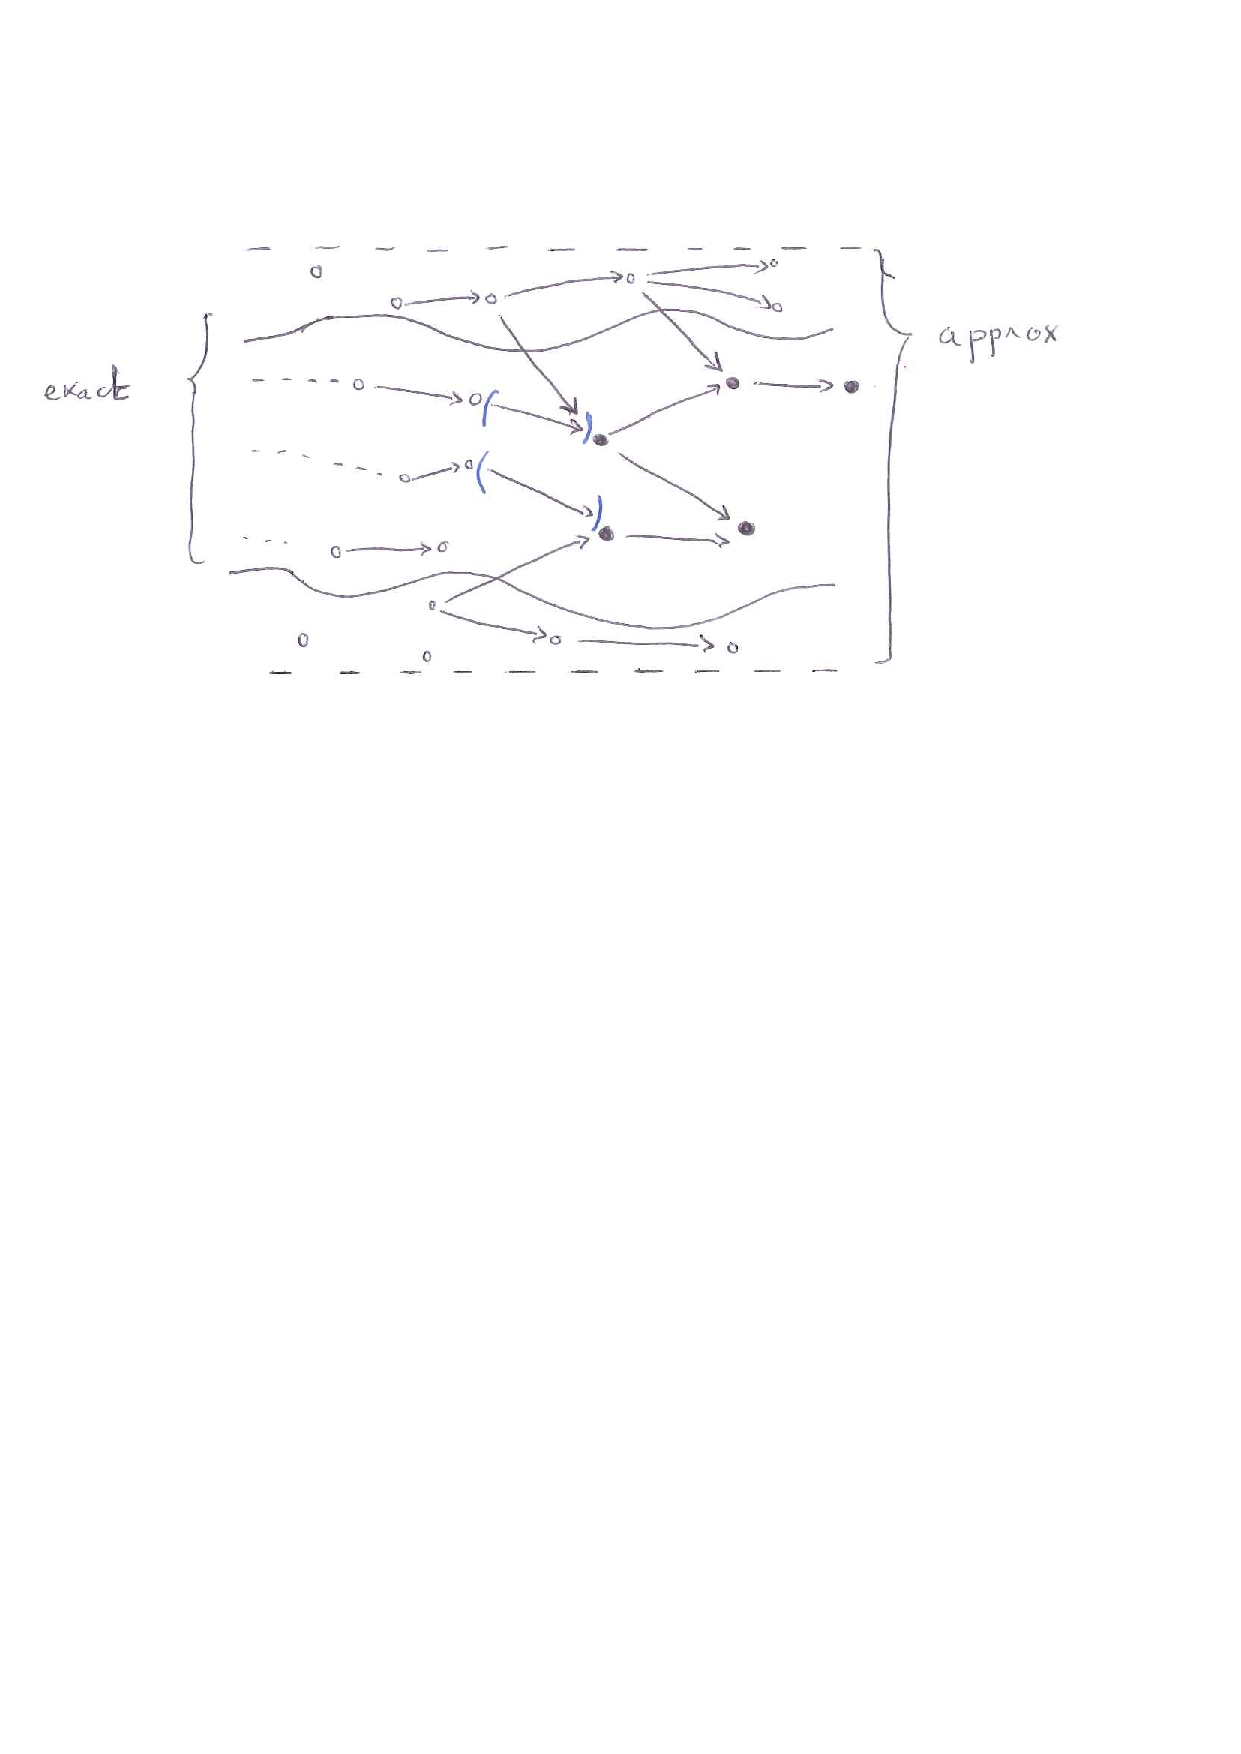
\includegraphics[width=12cm]{4_contre_ex/illustration}
  \caption{\footnotesize }
  \label{fig:illustration}
\end{figure}
Ainsi dans la figure~\ref{fig:illustration}, si les états noirs ont été introduits avant de considérer les transitions
entre parenthèses, on ne peut être sûr que ces états et leur successeurs sont atteignables tant que 
ces transitions n'ont pas été considérées par l'exploration.

Cette technique permet de réduire considérablement la zone d'incertitude en cas d'échec.
Lorsque la vérification de la propriété échoue à cause d'un état $s$ dont on est sûr
qu'il appartienne au système, on peut conclure que le système viole la propriété:
l'état $s$ constitue un \emph{contre-exemple}. Dans le cas contraire on ne sait toujours rien dire,
on est  dans le cas soit d'une fausse alarme soit d'un contre-exemple.

\section{Principe de l'approche à la {CEGAR} appliqué au model-checking régulier}

Il est possible d'améliorer l'approche précédente, en exploitant l'information
lorsque la vérification échoue et que l'on ne peut pas conclure à un contre-exemple ou une fausse alarme.
En effet, si l'on n'est pas sûr qu'un état $s_?$ est atteignable, alors il a été introduit par une étape d'accélération.
Pour cet état $s_?$, on peut envisager les deux situations suivantes:
% En fonction de la réelle nature de chaque état supprimé on peut différencier
% deux cas possibles~:

\begin{itemize}
\item
  Soit $s_?$ n'est pas réellement atteignable: raffiner l'approximation de façon
  à supprimer $s_?$ est correct, puisqu'il s'agit d'une fausse alarme.
\item
  Soit $s_?$ est atteignable: il existe au moins une exécution du système qui passe par cet état~:
  cela signifie qu'au moment où la propriété a été violée, la trace correspondant à l'exécution
  n'a pas encore été considérée, mais l'état est la conséquence d'une étape d'accélération. 
  Si même si on retire $s_?$ de l'approximation, comme il est atteignable, on finira toujours
  par produire le terme par des étapes de calcul exact. 
\end{itemize}
On peut donc envisager de supprimer l'état $s_?$ de l'approximation, si l'on tente de compléter à nouveau
l'ensemble des états atteignables. C'est le principe de l'approche à la {CEGAR}
(\emph{Counter-Example Guided Abstraction Refinement})~\cite{DBLP:conf/time/Clarke03}: on retire successivement tous les
états $s_?$ qui conduisent à la mise en échec de la propriété s'il n'est pas possible
de déterminer s'ils sont des contre-exemples ou non. Chaque phase de raffinement conduit 
alors à la reprise du calcul de l'ensemble des atteignables privé des états $s_?$.
Cependant, raffiner l'approximation de l'ensemble des états peut entraîner une divergence du calcul
puisque le raffinement affaiblit l'approximation~: cela impose de raffiner avec parcimonie, pour
éviter d'accroître ce risque de divergence.


Dans~\cite{DBLP:conf/cav/BouajjaniHV04}, Bouajjani et al. ont introduit les premières
techniques à la CEGAR pour le model-checking régulier, avant de
l'étendre aux termes dans~\cite{BouajjaniHRV-Infinity06,BouajjaniHRV-SAS06}. 
Le principe de ces travaux repose sur une pile qui contient tous les automates d'arbres
intermédiaires produits par le calcul depuis l'automate initial.
La relation de transition est définie par $T$ un transducteur d'automates
d'arbres~\cite{TATA}. L'abstraction est construite en utilisant des prédicats 
qui paramètrent les étapes d'accélération.
Les prédicats sont représentés par des automates d'arbres.

Le processus de calcul est basé sur l'alternance étape de transduction
suivie d'une étape d'abstraction. Pour déterminer si un terme
est un contre-exemple ou un terme suspicieux\footnote{\footnotesize un terme dont on ne peut
déterminer si il est atteignable ou non}, l'approche repose sur un
calcul arrière qui impose de construire la relation de transition
inverse $T^{-1}$. À partir d'un ensemble $X_n$ de termes reconnus dans l'automate $M_n$ tels que $X_n$
viole une certaine propriété, on cherche dans les automates précédents quels termes ont permis par $T$
de produire les termes de $X_n$. Pour cela, on calcule un sur-ensemble des prédécesseurs possibles, 
et on recherche ceux qui étaient effectivement reconnus par l'automate $M_{n-1}$, (calcul d'intersection)
ce qui constitue l'ensemble de termes $X_{n-1}$. On recommence le processus jusqu'à:
\begin{itemize}
\item obtenir l'ensemble $X_0 \not= \emptyset$ dont l'un des termes est reconnu par l'automate initial,
  permet de produire l'un des termes de $X_n$: l'ensemble  $X_n$ contient un contre-exemple.

\item obtenir $X^k = \emptyset$ pour $k \le n$, on peut alors en déduire 
  que les termes de $X_{k+1}$ n'ont pas été produits par l'application du transducteur $T$ sur l'automate $M_k$.
  Ils sont donc le résultat d'une étape d'accélération réalisée sur l'automate $M_{k+1}$.
  Donc pour éviter les termes $M_n$, il faut retirer les termes de $M_{k+1}$ qui sont
  à l'origine de leur introduction en raffinant l'abstraction réalisée sur $M_{k+1}$.
\end{itemize}
Cette opération est d'autant plus coûteuse que la propriété est violée tardivement. 
Plus $n$ est grand, plus la recherche en arrière coûte cher, les opérations booléennes sur
les automates d'arbres ayant un coût non négligeable.


\begin{figure}[ht!]
  \centering
  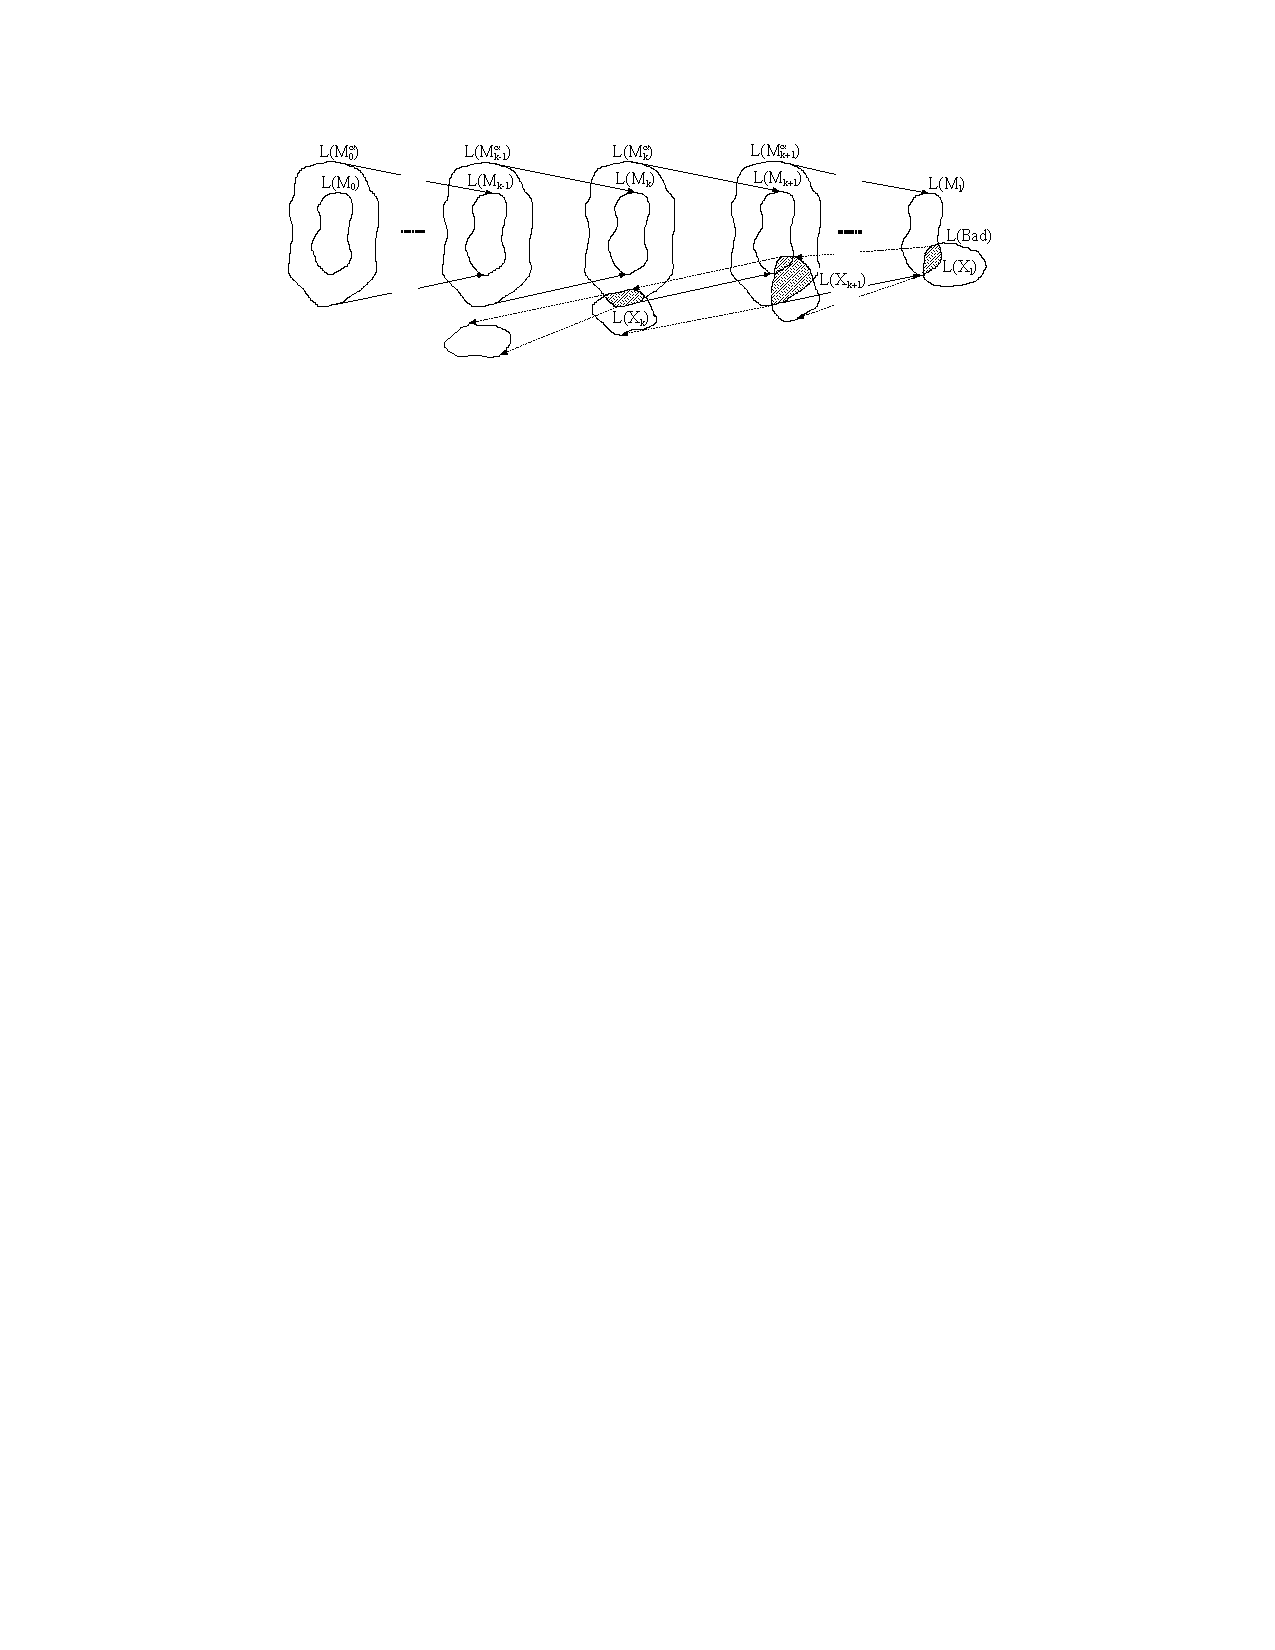
\includegraphics[width=14cm]{4_contre_ex/armc}
  \caption{\footnotesize Le calcul en arrière en model-checking régulier (fig. extraite de~\cite{DBLP:conf/cav/BouajjaniHV04})}
\end{figure}

Dans~\cite{BCHK08}, Boichut et al. ont tenté une approche similaire mais en utilisant des
règles de réécriture à la place des transducteurs et définissent l'abstraction des règles d'approximation
directement pour l'automate. De la même manière, le processus est basé sur la sauvegarde des automates
obtenus à chaque pas de calcul. Néanmoins, cette technique nécessite
que les règles de réécriture soient linéaires à gauche et à droite, pour effectuer le
calcul en arrière: la complétion d'automates d'arbres nécessite de
modéliser la relation de transition $Rel$ par un système de réécriture
linéaire à gauche, et le calcul arrière -- lui aussi réalisé par la
complétion -- nécessite la relation $Rel^{-1}$ définie en retournant
chaque règle $l \rw r \in \R$ en $r \rw l \in \R^{-1}$, imposant aux
membres droits dans $\R$ d'être linéaires.  Si la modélisation de
systèmes par un ensemble de règles de réécriture linéaires est
toujours possible, elle peut s'avérer moins immédiate qu'avec
des règles de réécritures linéaires à gauches.


%%%%%%%%%%%%%%%%%%%%%%%%%%%%%%%%%%%%%%%%%%%%%%%%%%%%%%%%%%%%%%%%%%%%%%%%%%%%%%%%%%%%%%%
%%%%%%%%%%%%%%%%%%%% VERSION EXTRAITE DE ../plan/plan_contre_ex.mm %%%%%%%%%%%%%%%%%%%%
%%%%%%%%%%%%%%%%%%%%%%%%%%%%%%%%%%%%%%%%%%%%%%%%%%%%%%%%%%%%%%%%%%%%%%%%%%%%%%%%%%%%%%%

\section{Contre-exemples et automates d'arbres}

% {Bouajjani \cite{artmc06}, Besançon \cite{fib:arra08}}
% {Approches intéressantes, mais limitées d'un point de vue complexité et expressivité}
% {Utilisation de l'inclusion d'automates d'arbres + intersection, systèmes linéaires à droite et
%   à gauche : ça n'est pas le cas du TRS de Java (non linéaire à droite) (pour éviter les calculs d'inclusion, calcul en arrière à partir de la propriété)}
% {Autres approches ? voir les papiers de Besançon ???}
%\bigskip
La contribution de ce chapitre est de proposer une solution pour améliorer
la complétion en cas d'échec et de proposer une procédure de raffinement
à la CEGAR pour l'algorithme de complétion d'automates d'arbres sans avoir recours 
au calcul en arrière pour déterminer si un terme est un contre-exemple ou non.
On espère ainsi gagner en performance par rapport aux techniques existantes.
Pour cela, on définit des automates d'arbres instrumentés que
l'on appelle \textbf{$\RE$-automates} et dont la sémantique 
nous informe sur la manière de réécrire les termes.
En résumé l'automate caractérise les termes ajoutés par réécriture
de $\R$ ou par réécriture de $\R$ modulo $E$ en gardant une trace
des équations utilisées pendant l'accélération.
On propose alors une procédure de complétion d'un $\RE$-automate
pour $\R$ un système de règles linéaires à gauche et un ensemble d'équations $E$.
L'information nécessaire étant maintenue à jour dans le $\RE$-automate courant, 
il n'est plus nécessaire de revenir sur les calculs antérieurs pour
connaître la nature d'un terme: l'exécution de l'automate pour un terme $t$
permet d'obtenir des informations sur l'atteignabilité. L'automate constitue en lui-même
la procédure de semi-décision.
Pour un terme $t$ reconnu par le $\RE$-automate, la sémantique informe des différentes étapes
d'accélération qui ont été nécessaire à sa construction. Lorsque l'automate indique qu'il n'y a
pas eu d'abstraction pour obtenir $t$, le terme est atteignable par $\R$.  Dans le cas
contraire, on dispose de l'information nécessaire pour raffiner efficacement l'approximation par la procédure 
d'élagage du $\RE$-automate que l'on propose.
De plus, nous verrons que la technique de raffinement développée ici est plus
précise que celle présentée dans~\cite{BCHK08}, ce qui lui permet  
converger plus fréquemment. Enfin, ce travail étend les abstractions
équationnelles~\cite{MeseguerPM-TCS08,Takai-RTA04} pour la détection
de contre-exemples et le raffinement.

%%Our approach is naturally more efficient than the one of
%%Bouajjani et al. as it does not require to store the intermediary
%%computation steps and apply a reverse of the transition relation to
%%conclude whether the term is reachable or not.

%\paragraph{Related work.} 



\section{L'intuition initiale}
\label{sec:intuition}
L'idée qui a conduit à la l'introduction des $\RE$-automates peut être illustrée à l'aide de l'exemple~\ref{ex:intuition}.
\begin{example}
  \label{ex:intuition}
  Soit $\A$ un automate défini comme:
  \begin{itemize}
  \item $\Q_f = \{ q_g, q_f\}$
  \item $\Delta = \{ f(q_a) \rw q_f,\ g(q_b) \rw q_g,\ a\rw q_a,\ b\rw q_b\}$
  \end{itemize}
  L'automate reconnaît les termes $f(a)$ et $g(b)$.
  On applique à cet automate l'équation $a = b$ ce qui permet de fusionner les états $q_a$ et $q_b$
  \[\xymatrix{
    a \ar@{=}_{E}[r]\ar[d]_{\A}^{*} & b \ar[d]_{*}^{\A}\\
    q_a & q_b
  }
  \]
  On obtient l'automate $\A'$ formé par les transitions $\Delta' = \{ f(q_a) \rw q_f,\ g(q_a) \rw q_g,\ a\rw q_a,\ b\rw q_a\}$
  où $q_b$ est remplacé par $q_a$. Ainsi les termes $a$ et $b$ sont dans la même classe d'équivalence, ce qui a pour 
  conséquence d'ajouter les termes $f(b) \in \Lang(\A', q_f)$, et $g(a) \in \Lang(\A', q_g)$.
\end{example}

  La fusion produit bien l'effet escompté sur le langage reconnu. En revanche, lorsque l'on se place du point de vue
  de l'état $q_f$, la fusion ne permet pas de comprendre à posteriori que  $f(b)$ est obtenu par l'abstraction, 
  alors que $f(a)$ était déjà reconnu par $\A$. Dualement, on peut remarquer le même problème à l'état $q_g$ avec les termes
  $g(b)$ et $g(a)$.

  Une manière de pallier à cette limitation consiste à rendre explicites les opérations de fusion.
  La solution retenue consiste à remplacer le renommage par des $\varepsilon$-transitions particulières:
  \[\xymatrix{
    a \ar@{=}_{E}[r]\ar[d]_{\A}^{*} & b \ar[d]_{*}^{\A}\\
    q_a \ar@/^0.6pc/[r]^{=} & q_b \ar@/^0.6pc/[l]^{=}
  }
  \]
  Maintenant, on peut savoir si un terme a été ajouté au langage grâce à l'abstraction ou non, juste en considérant
  les transitions utilisées pour le reconnaître:

  \begin{example}
    \begin{description}
    \item $f(a) \lrw f(q_a) \lrw q_f$ indique $f(a)$ ne vient pas de l'abstraction,

    \item $f(b) \lrw f(q_b) \mathbf{\stackrel{=}{\lrw}} f(q_a) \lrw q_f$ est obtenu par l'abstraction.
    \end{description}
  \end{example}
  
  Cela est suffisant pour caractériser la relation de causalité liée
  aux étapes d'abstraction qui peuvent avoir lieu lors de la
  complétion de l'automate.  C'est sur ce principe que repose les
  $\RE$-automates introduits dans la section~\ref{sec:RE-automaton}.



\section{Définition d'un $\RE$-automate}
\label{sec:RE-automaton}

Un $\RE$-automate est une extension de la définition standard des automates d'arbres,
dont la sémantique donne des informations sur les termes reconnus par cet automate
notamment pour un problème d'atteignabilité. Elle permet en particulier 
de distinguer les termes pour lesquels l'atteignabilité est sûre des autres termes.
Définir un $\RE$-automate n'a donc de sens que dans le cadre d'un problème d'atteignabilité 
donné $(I, \R, Bad)$ et d'une abstraction définie par un ensemble $E$ d'équations. 
On notera que le cas particulier du calcul exact
dénoté par $E = \emptyset$ est couvert par l'approche, mais ne se révèle pas intéressant puisque
le problème soulevé n'existe que dans le cas d'une sur-approximation.

Soit un problème d'atteignabilité défini dans l'ensemble de termes $\TF$ avec 
$I$ comme ensemble fini de termes initiaux $\R$ un ensemble de règles de réécriture
et $E$ un ensemble d'équations.

% $\Deq$ denotes a subset
% of the equivalence relation induced by the set of equations.
% Moreover, we will be able to know that a term recognized using a
% transition of $\Deq$ is the result of a widening step.  The
% example~\ref{ex:semantics} illustrates the principle of a
% $\RE$-Automaton.


%We now give the formal definition for $\RE$-automata.

\begin{definition}
  \label{def:re-automaton}
  Un \textbf{$\RE$-Automate} est un automate d'arbres défini comme un quadruplet de la forme
  $\A= \langle \F, \Q, \Q_F,\Delta \cup \Drw \cup \Deq\rangle$,
  avec $\Q_F \subseteq \Q$ et composé de 3 ensembles de transitions distinctes~:

  \begin{description}
  \item $\Delta$ est un ensemble de transitions normalisées (\textit{c.f.} définition~\ref{def:transitions}),
  \item $\Deq$ est un ensemble de $\varepsilon$-transitions,
  \item $\Drw$ est un ensemble de 
  $\varepsilon$-transitions étiquetées par $\top$ ou par une conjonction de prédicats de la forme $Eq(q, q')$ 
  avec $q, q' \in \Q$, et $q \rw q' \in \Deq$.
  \end{description}
\end{definition}


Un $\RE$-automate est un automate d'arbre dans lequel les transitions sont classées en trois catégories.  D'une part les
transitions normalisées et deux ensembles distincts de $\varepsilon$-transitions~:
\begin{itemize}
\item les premières caractérisent la relation de réécriture qui peut exister entre les classes
  d'équivalence de l'automate, comme les $\varepsilon$-transitions produites par la complétion~\ref{sec:completion}, 
  mais étiquetées par des formules logiques.

\item les secondes définissent la relation d'abstraction qui peut exister entre deux classes d'équivalence comme illustré en 
  section~\ref{sec:intuition}.
\end{itemize}

% Comme pour les $\R$-automates, la sémantique d'un $\RE$-automate n'a de sens que dans le contexte d'un problème d'atteignabilité
% constitué d'un ensemble initial, d'un système de réécriture, et d'un ensemble d'équations
% \footnote{\footnotesize l'ensemble des équations peut être éventuellement vide, mais on se ramène alors au cas du calcul 
%   sans approximation couvert par les $\R$-automates.}.


\begin{example}
  \label{ex:semantics}
  Soit $\A$ un $\RE$-automate reconnaissant dans l'état final $\mathbf{q_f}$
  le système $(\F, I, \R)$ défini par 

  $I = f(a)$, $\R = \{f(c) \rw g(c),\ a \rw b\}$, et un ensemble d'équations $E = \{ b = c\}$.

  Dans $\A$, l'égalité $b = c$ est symbolisée par les 2 transitions $q_c
  \rw q_b$ et $q_b \rw q_c$ de $\Deq$, en tenant compte que $b$ et $c$
  sont respectivement reconnus dans les états $q_b$ et $q_c$.
  
  Ainsi du point de vue de l'état $q_c$, la transition $q_b \rw q_c$
  nous indique que le terme $b$ est obtenu à partir du terme $c$ par égalité.
  On peut constater que la transition $q_c \rw q_b$ nous permet 
  de conclure réciproquement que le terme $c$ est obtenu à partir du terme $b$.

  Les transitions $q_g \rw q_f$ et $q_b \rw q_a$ dénotent des étapes de réécriture.
  De la même manière que pour les transitions qui dénotent l'équation $b=c$, du point
  de vue de l'état $q_a$, la transition $q_b \rw q_a$ permet de déduire que le terme
  $b$ est un descendant par $\RE$ du terme $a$. La transition $q_g \rw q_f$ indique 
  aussi à l'état $q_f$ que le $g(c)$ est un descendant de $f(a)$ par $\RE$.

  Les deux transitions $q_g \rw q_f$ et $q_b \rw q_a$ permettent de déduire que l'on a $f(a) \rw^*_\RE g(c)$
  et $a \rw^*_\RE b$. En revanche, lorsqu'on déplie la relation $f(a) \rw^*_\RE g(c)$, on obtient la chaîne
  $f(a) \rw_\R f(b) =_E f(c) \rw_\R g(c)$, qui utilise l'égalité $b = c$ pour passer de $g(b)$ à $g(c)$, relation que l'on peut 
  déduire de la transition $q_c \rw q_b$. Ainsi, on étiquette la transition $q_g \rw q_f$
  avec la formule $Eq(q_c, q_b)$ pour reporter cette information. 
  D'autre part, la transition $q_b \rw q_a$ est étiquetée avec $\top$ ce qui signifie 
  qu'aucune égalité n'est utilisée pour réécrire $a$ en $b$: de cette transition, on déduit $a \rw^*_\R b$.
  \begin{center}
    %\centering
    \tikz[thick, scale=1]{
      \node (qf) at (0, 0)   {$\mathbf{q_f}$};
      \node (qg) at (4, 0)   {$q_g$};
      \node (f)  at (0,-1.5) {$f(\;q_a\;)$};
      \node (g)  at (4,-1.5) {$g(\;q_c\;)$};
      \node (qa) at (0,-2.8) {$q_a$};
      \node (qb) at (2,-2.8) {$q_b$};
      \node (qc) at (4,-2.8) {$q_c$};
      \node (a)  at (0,-4.3) {$a$};
      \node (b)  at (2,-4.3) {$b$};
      \node (c)  at (4,-4.3) {$c$};
      % \Delta
      \draw [->] (f) edge (qf);
      \draw [->] (g) edge (qg);
      \draw [->] (a) edge (qa);
      \draw [->] (b) edge (qb);
      \draw [->] (c) edge (qc);
      % liens de descendance
      \draw [dashed] (f) edge (qa);
      \draw [dashed] (g) edge (qc);
      % \Drw
      \draw [->, bend right=15] (qg) to node[auto, swap] {\footnotesize$Eq(q_c, q_b)$} (qf);
      \draw [->, bend right=15] (qb) to node[auto, swap] {\footnotesize$\top$} (qa);
      % \Deq
      \draw [->, bend right=15] (qb) to node[auto, swap] {\footnotesize$=$} (qc);
      \draw [->, bend right=15] (qc) to node[auto, swap] {\footnotesize$=$} (qb);
    }
  \end{center}
  %\caption{Example of $\RE$-automaton}
\end{example}

%%% Local Variables: 
%%% mode: latex
%%% TeX-master: "../main"
%%% TeX-PDF-mode: t
%%% End:



% Les $\RE$-automates sont une extension des $\R$-automates introduits dans
% \cite{BoyerG-RULE09}. 

Intuitivement, dans un $\RE$-automate, les termes sont reconnus en utilisant les transitions de $\Delta$, les transitions de $\Drw$ dénotent la relation de réécriture
entre ces termes, et les $\varepsilon$-transitions de $\Deq$ dénotent
les étapes d'abstraction. Chaque transition de $\Drw$ est étiquetée par une formule logique
correspondant aux approximations réalisées pour produire l'étape de réécriture. 
Plus exactement, la formule indique quelles sont les étapes d'abstraction qui ont été nécessaires 
pour produire le terme qui a pu être réécrit. 
% Plus exactement, 
% La relation caractérisée est semblable à celle dénotées par les automates obtenus par la complétion:
Ainsi, lorsque la formule est $\top$, aucune approximation n'est nécessaire et le terme
est atteignable simplement par réécriture, sinon le terme a été produit par réécriture 
modulo $E$. Dans~\cite{GenetR-JSC10}, les auteurs établissent déjà le lien entre la réécriture $\RE$
et les automates produit par la complétion.


%\comments{Sinon, si la formule n'est pas équivalente à $\top$, th}


\subsection{Sémantique}


% We introduce $\f^=$ which denotes the transitive closure of transitions of $\Delta \cup \Deq$.
% The couple $(Q, \f^=)$ induces the equivalence relation such that if terms $u$ and $v$
% are in the same equivalence classe, then $u =_E v$.

%%%%%%%%%%%%%%%%%%% FSTTCS %%%%%%%%%%%%%%%%%%%%%%%%


%\comments{On s'en sert?: In the following, we assume that logical
%formulas are always transformed into an equivalent \emph{Disjunctive Normal
%  Form} using standard logic equivalences.} \noindent 
%%Normalized transitions of $\Delta$ in a $\RE$-automaton recognize terms, called
%%{\em representative}, whereas $\varepsilon$-transitions represent rewriting and
%%equivalence relations between them. 

%%\comments{Axel: shall we keep the definition of sets of representative?}

Dans la suite, on utilisera $\rw_\Delta$ pour dénoter la clôture transitive et réflexive de 
la relation induite par les transitions de tout ensemble $\Delta$. 
Dans le cas où $\Delta$ est l'ensemble de toutes les transitions normalisées on utilisera $\rwne$ 
pour $\rw_\Delta$. 
Pour $\Delta$ un ensemble donné de transitions normalisées d'un $\RE$-automate, 
on définit l'ensemble des représentants d'un état comme $Rep(q) = \{ t \in \TF | t \rwne q\}$. 
On introduit maintenant la définition formelle des exécutions d'un $\RE$-automate.

%This $\rwned$ is a particular case of the new rewriting relation $\xrw{\alpha}_\A$
%of $\RE$-automata. 

\begin{definition}
  \label{def:xrw_alpha}
  On définit l'\textbf{exécution du $\RE$-automate} $\A$ sur le terme $t \in \TFQ$ reconnu en l'état $q$ 
  par la relation $t \xrw{\alpha}_\A q$ définie comme:
  \begin{itemize}
  \item $t|_p = f(q_1, \dots, q_n)$ et $f(q_1, \dots, q_n) \rw q \in \Delta$
    alors $t \xrw{\top}_\A t[q]_p$
  \item $t|_p = q$ et $q \rw q' \in \Deq$ alors $t \xrw{Eq(q, q')}_\A t[q']_p$
  \item $t|_p = q$ et $q \xrw{\alpha} q' \in \Drw$ alors $t \xrw{\alpha}_\A t[q']_p$ 
%     where $\alpha = \left\{
%       \begin{array}{ll}
%         \alpha_k &\textrm{if } 1 \le k \le n \land \phi = \bigvee_1^n \alpha_i\\
%         \top &  \textrm{if } \phi = \top
%       \end{array}\right.
%     $
  \item $u \xrw{\alpha}_\A v$ et  $v \xrw{\alpha'}_\A w$ alors $u \xrw{\alpha \land \alpha'}_\A w$
  \end{itemize}
\end{definition}

\noindent
Une exécution $\xrw{\alpha}$ abstrait une séquence de réécriture de $\rwmod$. Si $t
\xrw{\alpha} q$, alors il existe un terme $s\in Rep(q)$ tel que 
$s\rwmod^* t$. La formule  $\alpha$ dénote le sous-ensemble de transitions de $\Deq$ 
utilisées pour reconnaître $t$ dans $q$.


%%i.e. the equivalence
%%steps, induced by $E$, needed to rewrite $s$ into $t$ using
%%$\rwmod$.
\begin{example}
  On considère le $\RE$-automate $A$ de l'exemple \ref{ex:semantics}, puis la transition
  $g(b) \xrw{Eq(q_b, q_c) \land Eq (q_c, q_b)} q$: on sait qu'il existe 
  une séquence de réécriture $\rwmod$ à partir de $f(a)$, l'unique terme
  de l'ensemble des représentants de  $Rep(q)$, pour produire $g(b)$. 
  La formule indique que cette séquence de réécriture utilise 
  la relation d'équivalence  induite par $b = c$ dans les deux sens
  (transitions $q_b \rw q_c$ et $q_c \rw q_b$).
\end{example}


La relation $\xrw{\alpha}$ correspond à la relation standard de réécriture 
(\textit{c.f.} la section~\ref{sec:automates}) d'un automate d'arbres instrumenté avec
des formules logiques.

\begin{theorem}\label{th:equiv}{\quad\quad
  $\forall t\in\TFQ,\; q \in \Q,\; t \xrw{\alpha}_\A q \equ t \rw_\A^* q$}
\end{theorem}

\begin{proof}
  La preuve est simple et peut se réaliser par induction en montrant qu'il suffit
  d'ignorer les formules qui sont manipulées par la définition~\ref{def:xrw_alpha},
  pour retrouver la relation originale $\rw_\A$. 
\end{proof}

Ce théorème est rassurant puisque les $\RE$-automates ont la même expressivité
que les automates d'arbres, ce qui permet de rester dans la classe des langages réguliers
de termes. Ce point est important puisqu'on ne perd pas d'expressivité pour représenter les
approximations. D'autre part, puisqu'on ne gagne pas en expressivité
non plus, on évite le coût du passage à des classes de langages non réguliers
comme c'est le cas par exemple pour des automates à contraintes~\cite{TATA}.


On s'intéresse maintenant aux $\RE$-automates {\em bien-définis}. 
La propriété de bonne définition permet d'assurer que l'information
qu'apporte les $\RE$-automates est correcte par rapport à la réécriture
par $\R$ et $E$. La propriété de bonne définition est nécessaire pour s'assurer 
lors du raffinement que l'on distinguera correctement les contre-exemples des faux-positifs.

% \comments{plus précis que la relation de $\RE$-cohérence, et sera simplement admise dans ce chapitre...}

\begin{definition}[Un $\RE$-automate bien-défini]
  \label{def:well-defined}
  $\A$ est un $\RE$-automate \emph{bien-défini}, si :
  % The second point of the definition is used to refine the $\RE$-automaton: a rewriting step of $\rwmod$
  % denoted by $q \xrw{\phi} q'$ holds thanks to the subset of transitions of $\Deq$
  % occurring in $\phi$. If we remove the transitions of $\Deq$ such that $\phi$
  % does not hold, then the transition $q \xrw{\phi} q'$ disappears and the term is 
  % no longer recognized.
  \begin{itemize}
  \item Pour tout état $q$ de $\A$, et tout terme $v$ tel que
    $v \xrw{\top}_\A q$, il existe $u$ un terme représentatif
    de $q$ tel que $u \rw^*_\R v$
  \item Si $q \xrw{\phi} q'$ est une transition de $\Drw$, alors il existe deux termes
    $s,t\in \TF$ tels que $s\xrw{\phi}_\A q$, $t\xrw{\top}_\A q'$
    et $t \rw_\R s$.
  \end{itemize}
\end{definition}

\noindent
Le premier point de la définition~\ref{def:well-defined} assure que
tout terme reconnu en utilisant uniquement des transitions étiquetées
par la formule $\top$ est atteignable à partir de l'ensemble initial.
Le second point est utilisé pour raffiner l'automate. Une séquence de réécriture
$\rwmod$ dénotée par $q \xrw{\phi} q'$ est possible grâce à certaines transitions
de $\Deq$ caractérisées par $\phi$. Si on supprime ces transitions de $\Deq$ de telle sorte
que $\phi$ devienne fausse, alors la transition $q \xrw{\phi} q'$ sera aussi supprimée.

A partir de cette définition, un terme $t$ qui est reconnu en 
utilisant au moins une transition étiquetée avec une formule différente de $\top$
peut être enlevée du $\RE$-automate en supprimant des transitions de $\Deq$.
Cette opération d'``élagage''  est illustrée ci-dessous.

\begin{example}
  \label{ex:pruning}
  On reprend le $\RE$-automate $\A$ de l'exemple~\ref{ex:semantics}.
  Cet automate reconnaît le terme $g(c)$. En effet, d'après la
  définition~\ref{def:xrw_alpha}, on a $g(c) \xrw{Eq(q_c, q_b)}
  q_f$. On considère maintenant la séquence de réécriture $f(a) \rw_\R f(b) =_E f(c) 
  \rw_\R g(c)$. On peut voir que si l'étape $f(b) =_E f(c)$ dénotée par la 
  transition $q_c \rw q_b$ est supprimée, alors $g(c)$ devient non-atteignable. 
  La première étape de l'élagage de $\A$ consiste donc à retirer cette
  transition. Dans un deuxième temps, on propage cette information en retirant
  toutes les transitions de $\Drw$ étiquetées par une formule construite avec le prédicat $Eq(q_c, q_b)$.
  Cela permet de supprimer tous les termes obtenus par réécriture en utilisant l'équivalence $b =_E c$.
  Suite à l'élagage, on constate que $\A$ ne caractérise plus que l'ensemble des termes $\{f(a), f(b)\}$.
\end{example}

%%As we shall see, the prunning technique sketched in the above example
%%will serve as a basis for the refinement technique presented in
%%section~\ref{sec:refinement}.


% Ici il y a 2 relations plus ou moins forte dans le cas ou $\Delta_\R$ un ensemble de termes infinis ou non...

%\subsection{Exemple de $\RE$-automate}

%\section{Equivalence entre la nouvelle sémantique et la sémantique standard}


\section{Construire un $\RE$-Automate pour le problème d'atteignabilité}


Dans cette section, on étend les principes de complétion et d'élargissement
présentés dans la section~\ref{sec:completion} aux $\RE$-automates. On parlera 
alors de \textbf{$\RE$-complétion}. Pour cela, on considère dans toute la section,
un ensemble $\R$ de règles de réécriture et une approximation définie par $E$ l'ensemble d'équations.
On veut produire un $\RE$-automate $\aapprox$  clos par réécriture à partir de $I$,
l'ensemble des termes initiaux caractérisé par l'automate $\Lang(\A) = I$.
Le $\RE$-automate $\aapprox$ est obtenu à partir de $\aaexeq^0$ en calculant
successivement les approximations $\aaexeq^i$, jusqu'à obtenir un point fixe
$\Lang(\aaexeq^{k+1}) \supseteq \Lang(\aaexeq^{k})$. Le $\RE$-automate $\aaexeq^{i+1}=\widen(\compl(\aaexeq^i))$
est $\aaexeq^i$ après une phase de complétion $\compl$ et suivie d'une phase d'accélération $\widen$.


\subsection{Construction de $\aaex^0$}

On définit le $\RE$-automate $\aaexeq^0 = \la \F, \Q^0, \Q_F, \Delta^0\ra$ tel que
le langage de $\aaexeq^0$ est exactement l'ensemble $I$. Cela revient à prendre 
l'automate $\A$ auquel on ajoute les deux ensembles vides pour $\Drw^0$ et $\Deq^0$, ce qui
est raisonnable puisque les termes de $I$ sont obtenus sans réécriture ni approximation.
Par construction, $\aaexeq^0$ est bien-défini.

\begin{property}
  $\aaexeq^0$ est bien-défini.
\end{property}

\begin{proof}
  $\aaexeq^0 = \la \F, \Q^0, \Q_f, \Delta^0 \cup \emptyset \cup \emptyset\ra$
  respecte de la définition~\ref{def:well-defined}, seulement si les deux points
  de la définition~\ref{def:well-defined} sont vérifiés.
  \noindent
  On sait que $\aaex^0$ ne possède aucune $\varepsilon$-transitions.
  Tous les termes sont reconnus au seul moyen des transitions de $\Delta^0$.
  Cela signifie que pour tout état $q$ l'ensemble des termes se définit comme $\{ t \in \TF | t \rw_{\Delta^0} q\}$.
  qui est égal à $Rep(q)$, l'ensemble des représentants de l'état $q$.
  On constate aussi que pour tout terme $t$, $t \rw_{\Delta_0} q$ implique $t \xrw{\top}_{\aaexeq^0} q$:
  le second et le troisième point de la définition~\ref{def:xrw_alpha}, ne sont pas utilisés, puisqu'il
  n'y a aucune $\varepsilon$-transition dans $\aaexeq^0$.
  % $\Drw^0$ et $\Deq^0$ sont vides.
  
  Le premier point de la définition~\ref{def:well-defined} est assuré: 
  pour tout état $q$, et tout terme $t \xrw{\top} q$, on a $t \in Rep(q)$, 
  et $t \rwR^* t$ par réflexivité. En particulier, si $q \in \Q_f$ est un 
  état final, alors le terme $t$ est un terme initial, donc atteignable.

  Quant au second point de la définition~\ref{def:well-defined}, il est assuré par $\aaex^0$ puisque $\Drw^0$ est vide.
\end{proof}

On s'intéresse maintenant à la construction de $\aaexeq^{i+1}$, soit à la $\RE$-complétion à proprement parler, ce
qui requiert la redéfinition des fonctions $\compl$ et $\widen$. Cela est dû à la prise en compte des formules
qui doivent être ajoutées pour chaque transition de $\Drw$ ajoutée au $\RE$-automate.

% COn va donc caractériser les paires critiques par un triplet de la forme  $\la q, r\sigma, \alpha\ra$
% alors le problème de la paire critique comme

\section{L'étape de $\RE$-complétion $\compl$}
% On considère le $\RE$-automate $\aaexeq^i = \la \F, \Q^i, \Q_f, \Delta^i \cup \Drw^i \cup \Deq^i \ra$ obtenu
% après $i$ étapes de complétion-approximation.

Une étape de $\RE$-complétion consiste à construire le $\RE$-automate $\compl(\aaexeq^i)$ que l'on obtient à partir de $\aaexeq^i$ et $\R$.
Toute étape de $\RE$-complétion assure que:

\begin{itemize}
\item $\Lang(\compl(\aaexeq^i)) \supseteq \Lang(\aaexeq^i)$
\item $\forall t \in \Lang(\aaexeq^i)$, si $t \rw_\R t'$ alors $t \in \Lang(\compl(\aaexeq^i))$
\item si $\aaexeq^i$ est bien-défini, $\compl(\aaexeq^i)$ l'est aussi.
\end{itemize}


Comme expliqué précédemment dans la section~\ref{sec:completion}, la complétion est basée sur
la recherche et la résolution des paires critiques qui existent entre les transitions de l'automate 
et $\R$. Dans le cas de la $\RE$-complétion, le principe reste le même. Cependant, on considère
que pour un $\RE$-automate les paires critiques sont caractérisées par un triplet $\la q, r\sigma, \alpha\ra$
où $\alpha$ est une formule telle que:
  \[
  \xymatrix{
    l\sigma \ar[dd]_{\aaexeq^i}^{\alpha} \ar[rr]_{\R} && r\sigma\\
    \\
    q
  }
  \]

On considère qu'une telle paire critique n'est pas résolue si il n'existe pas de formule $\alpha'$ telle que 
le diagramme ci-dessous commute:
  \[
  \xymatrix{
    l\sigma \ar[dd]_{\aaexeq^i}^{\alpha} \ar[rr]_{\R} && r\sigma \ar@/^1.8pc/[ddll]_{\alpha'}^{\aaexeq^i}\\
    \\
    q
  }
  \]

Pour résoudre une telle paire critique, on ajoute au $\RE$-automate $\compl(\aaexeq^i)$
de nouvelles transitions pour avoir $r\sigma \xrw{\alpha}_{\compl(\aaexeq^{i})} q$.
Plus formellement, on peut définir la résolution d'une paire critique de la manière suivante~:
%$p=\la r\sigma, \alpha, q\ra$. 

\begin{definition}{Résolution d'une paire critique}
  \label{def:resolution_cp}
  On considère la paire critique $p=\la r\sigma, \alpha, q \ra$ qui est non résolue dans
  $\aaexeq^i \la \F, \Q, \Q_f, \Delta\cup \Drw\cup \Deq \ra$.
  La paire critique $p$ est résolue $p$ dans le $\RE$-automate $\compl(\aaexeq^i)$
  si $\compl(\aaexeq^i) = \la \F, \Q', \Q_f, \Delta'\cup \Drw'\cup \Deq \ra$ avec:
  \begin{itemize}
  \item $\Delta'\supseteq \Delta \cup \norm(r\sigma,\Delta\setminus \Delta^0)$
  \item $\Drw'\supseteq \Drw \cup \{q' \xrw{\alpha} q\}$ avec $q'$ un état tel que $r\sigma \rw^*_{\Delta'} q'$
  \item $\Q' \supseteq \Q$ contient les nouveaux états de $\Delta'$ produits par la normalisation.
  \end{itemize}
\end{definition}

On ajoute alors les transitions telles qu'il existe un état $q'$ avec
$r\sigma \xrw{\top}_{\compl(\aaexeq^i)} q'$ et $q'\xrw{\alpha} q \in \Drw'$. 
% $\Q_{new}$ un ensemble de nouveaux états tels que $\Q_{new} \cap \Q^i =\emptyset$.

On remarque que $\Delta^0$, l'ensemble des transitions initiales $\aaex^0$, n'est jamais utilisé
pour la normalisation de $r\sigma$. Ceci est nécessaire pour que la normalisation construise un ensemble de transitions
qui préserve la bonne définition du $\RE$-automate.
En effet, on doit imposer certaines contraintes aux transitions normalisées. Or ses contraintes
sont trop restrictives pour $\aaexeq^0$, qui ne pourrait plus représenter des ensembles infinis de termes initiaux.
Donc on exclut les transitions de $\Delta^0$ pour la normalisation.
% à l'ensemble de transitions utilisées par la normalisation. Mais ces contraintes limites considérablement
% l'expressivité de l'automate dans le cas il ne possède pas de $\varepsilon$-transitions: il n'est plus possible de
% reconnaître un langage infini. Pour ne pas limiter l'automate $\aaexeq^0$ aux ensembles finis et tout de même 
% maintenir la contrainte, on n'utilise pas les transitions de l'ensemble $\Delta^0$ lors de la normalisation.
% %C'est important pour préserver la bonne définition de $\A'$.
Le $\RE$-automate $\compl(\aaexeq^i)$ est obtenu en itérant ce
principe de résolution à toutes les paires critiques $p$ qui existent
entre $\R$ et $\aaexeq^i$. Cet ensemble de paires critiques peut être découvert
 en résolvant le {\em problème de filtrage} $l \match q$ pour chaque règle de
 réécriture $l \rw r\in \R$ et chaque état $q\in\aaexeq^i$.
L'algorithme de filtrage est détaillé plus tard dans la section~\ref{sec:filtrage}.

\section{La normalisation}
Comme dans le cas de la complétion, il n'est pas possible d'ajouter directement
la transition $r\sigma \xrw{\top}_{\compl(\aaexeq^{i})} q'$, elle peut ne pas être normalisée.
Une étape importante du calcul passe par la normalisation, qui assure notamment la bonne-définition
du futur $\RE$-automate $\compl(\aaexeq^{i})$. 
On s'intéresse donc tout d'abord à la normalisation et aux propriétés qu'elle doit assurer.
% More precisely, we add transitions
% $\norm(r\sigma,\Delta^i\setminus\Delta^0)$ (see Definition
% \ref{def:normalization}) to $\Delta^i$. Actually, the set of
% transitions $\Delta^i\setminus\Delta^0$ is deterministic and thus,
% after the normalization of $r\sigma$, there exists a state $q'$ with
% $r\sigma \xrw{\top}_{\compl(\aaexeq^{i})} q'$. Consequently, it remains to
% add the transition $q'\xrw{\alpha} q$ to $\Drw^{i}$. The whole process
% leads to the $\RE-$automaton $\compl(\aaexeq^i)$. This is formally defined as
% follows.



%%The transtion $r\sigma
%%\xrw{\top}_{\aaexeq^{i+1}} q'$ is actually build by adding normalized
%%transitions to $\Delta^{i+1}$ thanks to the {\em normalisation} of the
%%definition~\ref{def:normalization}.

\begin{definition}[Normalisation]
  \label{def:normalisation}
  La normalisation est réalisée en 2 étapes mutuellement récursives
  paramétrées par la configuration $c$ à reconnaître, et par $\Delta$ un ensemble de
  transitions à étendre.
  \[
  \left\{
    \begin{array}{lr}
      \norm(c, \Delta) = \slice(d, \Delta) & c \rw^!_\Delta d\textrm{, et }c,\ d \in \TFQ\\
      \slice(q,\Delta) = \Delta & q \in Q\\
      \slice(f(q_1,\dots, q_n), \Delta) = \Delta \cup \{f(q_1,\dots, q_n) \rw q\} & q_i \in \Q\textrm{ et }q \in \Q_{new}\\
      \slice(f(t_1,\dots, t_n), \Delta) = \norm(f(t_1,\dots, t_n), \slice(t_i, \Delta)) & t_i \in \TFQ \setminus \Q\\
    \end{array}
  \right.
  \]
\end{definition}

\noindent
Pour simplifier la définition, on ne manipule pas explicitement la mise à jour de l'ensemble des états $\Q$ de l'automate 
qui s'agrandit à chaque ajout de transitions. D'autre part, l'ensemble des nouveaux états $\Q_{new}$ est toujours considéré
comme disjoint de $\Q$, y compris lors de l'accroissement de $\Q$.

La définition de la normalisation est similaire à celle introduite dans la complétion d'automates d'arbres.
Cependant, les propriétés que l'on en attend sont différentes.
% , puisque l'on 
% exclut les transitions du $\RE$-automate initial (l'ensemble $\Delta^0$).

Lorsque l'on normalise, on suppose que $\Delta$ -- le second argument de $\norm$ -- est \textbf{déterministe}.

\begin{definition}
L'ensemble de transitions $\Delta$ est \textbf{déterministe}, si pour 
toutes transitions normalisées de la forme $f(q_1, \dots, q_n) \rw q$ et
$f(q_1, \dots, q_n) \rw q'$, alors on a $q = q'$.
\end{definition}

Comme la relation de réécriture induite par $\Delta$ est bien-fondée,
imposer le déterminisme à $\Delta$ permet d'assurer à tout terme $s
\in \TFQ$ de posséder une \textbf{unique forme normale} $t$ ce que l'on dénotera
par la relation $s \rw_\Delta^! t$.  Cette propriété requise par la
première étape de $\norm$ est aussi préservée lors de l'ajout de nouvelles transitions par $\slice$.
Lors de la première étape de complétion pour normaliser la première transition ajoutée
au $\RE$-automate $\aaexeq^0$, on prend $\Delta = \Delta^0 \setminus \Delta^0$ qui est
égal à l'ensemble vide, et est trivialement déterministe.

\begin{definition}
  On définit $\Delta$ comme \textbf{injectif}, si pour tout état $q$,
  il existe une seule transition de la forme $f(q_1, \dots, q_n) \rw q$.
\end{definition}
Cette propriété d'injectivité est importante pour assurer le premier point de la bonne-définition
d'un $\RE$-automate. L'exemple~\ref{ex:inj_contrex} illustre le problème posé
lorsque cette contrainte n'est pas respectée. Comme pour le déterminisme, l'injectivité
est une propriété préservée par la fonction $\norm$. De plus, pour $\aaexeq^0$, l'ensemble $\Delta = \emptyset$
est évidemment injectif.

\begin{example}
  \label{ex:inj_contrex}
  Soit le $\RE$-automate $\aaexeq^0$ défini par l'ensemble de transitions
  $\Delta^0 = \{ a \rw q,\ f(q)\rw q,\ g(q) \rw q_g\}$ et d'état final $q_g$.
  Le $\RE$-automate $\aaexeq^0$ reconnaît un ensemble infini de termes initiaux grâce à $\Delta^0$,
  en contrepartie $\Delta^0$ n'est pas injectif.
  On considère la règle de réécriture $g(x) \rw h(f(x))$. On va considérer la normalisation 
  avec et sans les transitions de $\Delta^0$. On résout la paire critique $\la q_g,\ h(f(q)),\ \top\ra$ 
  par les transitions $h(f(q)) \xrw{\top} q'$ et $q'\xrw{\top} q$. On tente de calculer $\norm(h(f(q)),\Delta^0)$ 
  alors que $\Delta^0$ n'est clairement pas injectif en $q$:
  \[\norm(h(f(q))),\Delta^0) = \slice(h(q),\Delta^0) = \Delta^0 \cup h(q) \rw q'\]
  On obtient alors le nouveau $\RE$-automate $\aaexeq^1$ tel que 
  \[\Delta^1 = \{a \rw q,\ f(q)\rw q,\ g(q) \rw q_g,\ h(q) \rw q'\}\textrm{ et } \Drw^1= \{ q' \rw q_g\}\]
  Pour le terme $h(a)$, on peut voir que $h(a) \xrw{\top} q_g$, ce qui signifie que $f(a)$ atteignable à partir de
  $\Lang(\aaexeq^0)$ par réécriture alors qu'il ne l'est clairement pas. Maintenant si on normalise sans tenir
  compte des transitions de $\Delta^0$:
  \begin{description}
  \item $\norm(h(f(q))),\emptyset) = \slice(h(f(q)),\emptyset) = \norm(h(f(q)), \slice(f(q),\emptyset))$
  \item $\slice(f(q),\emptyset) = \{f(q) \rw q_f\}$
  \item $\norm(h(f(q)), \{f(q) \rw q_f\}) = \slice(h(q_f), \{f(q) \rw q_f\}) = \{f(q) \rw q_f,\ h(q_f) \rw q'\}$
  \end{description}
  Dans ce cas, on a $\aaexeq^1$ de la forme 
  \[\Delta^1 = \{a \rw q,\ f(q)\rw q,\ g(q) \rw q_g,\ f(q) \rw q_f,\ h(q_f) \rw q'\}
  \textrm{ et } \Drw^1= \{ q' \rw q_g\}\]
  Alors on peut voir que tous les termes reconnus en $q'$ sont de la forme $h(f(x))$ et sont atteignables.
\end{example}

\begin{remark}
  Le calcul de la fonction $\norm(c, \Delta)$ termine. Pour caractériser la terminaison, on utilise
  une mesure $\mu : \TFQ \f \Nat$  qui compte le nombre d'occurrences de symboles de $\F$ de la configuration $c$.
  Exemple : $\mu(f(q_1, g(q_2), a)) = 3$. Toutes les preuves présentées dans la suite sont basées sur la décroissance
  stricte de $\mu(c)$ à chaque appel de $\norm$ ou de $\slice$.
  On définit inductivement cette mesure par:
  \begin{itemize}
  \item 
    $\mu(q) = 0$ si $q \in \Q$,
  \item 
    $\mu(f(t_1,\dots, t_n)) = 1 + \sum_1^n \mu(t_i)$.
  \end{itemize}
\end{remark}


\subsection*{Propriétés sur la normalisation}

\begin{property}%[Existence of a representative]
  \label{prop:norm_determinism}
  On pose  $\A = \la \F, \Q, \Q_f, \Delta \cup \Drw \cup \Deq\ra$, un $\RE$-automate tel que 
  $\Delta \setminus \Delta^0$ détermine l'ensemble déterministe de ses transitions, et $c \in \TFQ$ une configuration. 
  Si on a $\Delta' = \norm(c, \Delta \setminus \Delta^0)$,  alors il existe un état $q$ tel que  $c \rw^!_{\Delta'} q$.
\end{property}

\begin{proof}
  % Assuming $\F$ a set of symbols, and $\Q$ a set of states. 
  On définit $\A = \la \F, \Q, \Q_f, \Delta \cup \Drw \cup \Deq\ra$ et $c \in \TFQ$.
  On suppose également que $\Delta^1 = \Delta \setminus \Delta^0$ est déterministe.

  La première étape de calcul $\norm(c, \Delta^1)$ consiste à réécrire $c$ par
  $\Delta^1$ en sa forme normale notée $d$.   
  La seconde étape $\slice(d, \Delta^1)$ doit retourner $\Delta^2$ sur-ensemble de $\Delta^1$
  tel qu'il existe un unique état $q$ qui soit la forme normale de $d \rw^!_{\Delta^2} q$, et donc 
  par conséquent la nouvelle forme normale de $c$.
  La preuve est construite par induction sur la décroissance de $\mu(d)$.
  On considère les 3 cas de $\slice(d, \Delta^1)$ d'après la définition~\ref{def:normalisation}:
   
  \begin{enumerate}
  \item $\slice(q, \Delta^1) = \Delta^1$. Cela signifie que $d$ est déjà un état $q$. 
    Il n'y a rien à faire, $q$ est déjà la forme normale attendue,
    et $\Delta^2 = \Delta^1$ est déterministe.
  \item $\slice(f(q_1, \dots, q_n), \Delta^1) = \Delta^1 \cup \{ f(q_1, \dots, q_n) \rw q \sep q \in \Q_{new}\}$. 
    Chaque $q_i$ est un état. La configuration $f(q_1, \dots, q_n)$ peut être utilisée pour former le membre gauche d'une transition
    normalisée. On construit la nouvelle transition $f(q_1, \dots, q_n) \rw q$ en utilisant un nouvel état $q \in \Q_{new}$. 
    Le déterminisme est automatiquement préservé par l'ajout de cette transition à $\Delta^1$. On sait en effet
    que $d = f(q_1, \dots, q_n)$ est en forme normale, donc impossible à réécrire davantage par les transitions de 
    $\Delta^1$ : la nouvelle transition $f(q_1, \dots, q_n) \rw q$ est bien l'unique moyen de réécrire le terme $d$. On a donc construit
    $\Delta^2 = \Delta^1 \cup \{ f(q_1, \dots, q_n) \rw q \sep q \in \Q_{new}\}$ qui est déterministe, et $d \rw^!_{\Delta^2} q$.
     
   \item $\slice(f(t_1, \dots, t_n), \Delta^1) = \norm(f(t_1,\dots, t_n), \slice(t_i, \Delta^1)\ )$, $t_i \in \TFQ \setminus \Q$.
     Dans ce cas, on a choisi $t_i$ un sous-terme immédiat de $d$ qui n'est pas un état. Il en existe au moins un, sinon on se retrouve dans le cas précédent.
     Comme $t_i$ est un sous-terme de $d$ on peut en déduire $\mu(t_i) < \mu(d)$ d'après la définition de $\mu$.
     Par induction, $\Delta^1$ est étendu par $\slice(t_i, \Delta^1)$ pour obtenir $\Delta^3$ déterministe pour lequel il existe un état $q$ 
     tel que $t_i \rw^!_{\Delta^3} q$. En utilisant ce nouvel ensemble de transitions $\Delta^3$, on déplie $\norm(f(t_1,\dots, t_n), \Delta^3)$ 
     qui consiste dans un premier temps à réécrire le terme $f(t_1, \dots, t_n)$ par $\Delta^3$. On obtient une nouvelle configuration $f(t'_1, \dots, t'_n)$ où l'on sait
     au moins que le sous-terme $t_i'$ est égal à $q$ puisque le sous-terme $t_i$ peut être réécrit en $q$ par $\Delta^3$. On peut remarquer aussi
     que si certains des sous-termes de $t_i$ sont communs aux autres $t_j$ (les autres sous-termes immédiats de $d$), chaque $t_j$ sera aussi réécrit
     par $\Delta^3$ pour produire $t'_j$ la forme normale correspondante.
     Chaque étape de réécriture par $\Delta^3$ remplace un symbole de $\F$ par un état de $\Q$ par définition de la transition normalisée.
     Cette remarque permet de montrer $\mu(f(t_1,\dots,t_n) > \mu(f(t'_1,\dots,t'_n)$.
     Pour le sous-terme immédiat $t_i$, on sait que $\mu(t_i) > 0$ ($t_i$ n'est pas un état), et $\mu(t'_i) = 0$ ($t'_i$ est l'état $q$).
     Pour les autres sous-termes immédiats $t_j$ avec $j <> i$, on sait seulement $\mu(t_j) \ge \mu(t'_j)$ puisque $t_j \rw^!_{\Delta^3} t'_j$ 
     il peut ne pas y avoir eu réécriture nécessairement et donc $t_j = t'_j$.
     %il peut ne en utilisant les transitions de $\Delta^3$.
     On a $\mu(f(t_1,\dots,t_n) > \mu(f(t'_1,\dots,t'_n)$ par définition de $\mu$, et $f(t'_1,\dots,t'_n)$ est réécrit en sa forme normale par 
     l'ensemble $\Delta^3$ déterministe par hypothèse d'induction.
     Alors, on peut utiliser à nouveau l'hypothèse d'induction pour déduire que $\Delta^2 = \slice(f(t'_1,\dots,t'_n), \Delta^3)$
     étend $\Delta^2$ de façon à avoir l'état $q$ comme forme normale de $f(t'_1,\dots,t'_n) \rw^!_{\Delta^2} q$.
     Par transitivité, on a  $d \rw^!_{\Delta^2} q$ en utilisant l'ensemble déterministe $\Delta^2$ pour réécrire $d$ qui est égal à  $f(t_1, \dots, t_n)$.
   \end{enumerate}

   Finalement, on a montré que $\Delta^2 = \slice(d, \Delta^1)$ étend $\Delta^1$ en préservant le déterminisme tel qu'il existe un état 
   $q$ pour lequel $d \rw^!_{\Delta^2} q$. On sait aussi que $c \rw^!_{\Delta^2} d$. On peut conclure que $\Delta^2 = \norm(c, \Delta^1)$
   est déterministe, et qu'il existe un état $q$ tel que $c \rw^!_{\Delta^2} q$.
 \end{proof}

 \begin{property}[Normalisation et injectivité]
   \label{prop:norm_injectivity}
   Si $\Delta^1$ est injectif, alors $\norm(c \sep \Delta^1)$ l'est aussi.
 \end{property}

 \begin{proof}
   On pose le $\RE$-automate $A = \la \F, \Q, \Q_f, \Delta \cup \Drw \cup \Deq\ra$,
   la configuration $c \in \TFQ$, et l'ensemble de transitions normalisées $\Delta^1 = \Delta \setminus \Delta^0$ qui est injectif.
   
   En fait, d'après la définition de $\norm(c, \Delta^1)$, l'ajout des transitions est 
   uniquement réalisé lorsque l'on se trouve dans le cas $\slice(f(q_1,\dots,q_n), \Delta^1)$.
   La preuve se fait par induction comme pour la propriété précédente, à partir de l'étude de cas sur $\slice(d, \Delta^1)$:

   \begin{enumerate}
   \item $\slice(q, \Delta^1) = \Delta^1$. Cela signifie que $d$ est déjà un état $q$. L'injectivité est préservée.
     
   \item $\slice(f(q_1, \dots, q_n), \Delta^1) = \Delta^1 \cup \{ f(q_1, \dots, q_n) \rw q \sep q \in \Q_{new}\}$. 
     On utilise un nouvel état $q' \in \Q_{new}$, ce qui signifie que l'état n'est présent dans aucune transition
     de $\Delta^1$. La transition $f(q_1, \dots, q_n) \rw q'$ est donc l'unique transition de la forme $c \rw q'$,
     donc l'ensemble $\Delta^1 \cup \{ c \rw q'\}$ est injectif.

   \item $\slice(f(t_1, \dots, t_n), \Delta^1) = \norm(f(t_1,\dots, t_n), \slice(t_i, \Delta^1)\ )$, $t_i \in \TFQ \setminus \Q$
     Ici, on utilise l'hypothèse d'induction pour $\slice(t_i, \Delta^1)$ puisque $\mu (t_i) < \mu(f(t_1, \dots, t_n))$.
     Ce qui signifie que l'ensemble $\Delta' = \slice(t_i, \Delta^1)$ calculé est injectif.
     On regarde ensuite $\norm(f(t_1,\dots, t_n), \Delta')$. On sait d'après la propriété précédente, qu'il existe
     un état $q_i$ tel que $t_i \rw^*_{\Delta'} q_i$. On a alors $\norm(f(t_1,\dots, t_n), \Delta') = \slice(t, \Delta')$
     avec $t$ le terme $f(t_1,\dots, t_n)$ réécrit par $\Delta'$. On a $\mu (t) < \mu(f(t_1, \dots, t_n))$, donc en
     appliquant à nouveau l'hypothèse d'induction pour $\slice(t, \Delta^1)$ on obtient bien l'ensemble final $\Delta^2$ qui est injectif.
   \end{enumerate}

\end{proof}

De cette propriété, on peut alors en déduire la propriété suivante: 
\begin{property}
  \label{prop:norm_representant}
  Si la transition $r\sigma \rw_{\Delta^2} q'$ résulte de la normalisation $\Delta^2=\norm(r\sigma, \Delta^1)$
  avec $\Delta^1$ injectif, alors tous les représentants de l'état $q'$ sont de la forme $r\tau$, 
  avec $\tau: \X \rw \TF$.
\end{property}

\begin{proof}
  On pose le $\RE$-automate $A = \la \F, \Q, \Q_f, \Delta \cup \Drw \cup \Deq\ra$,
  tel que l'ensemble de transitions normalisées $\Delta^1 = \Delta \setminus \Delta^0$ est injectif.
  
  On considère que la transition $r\sigma \rw_{\Delta^2} q'$ résulte de la normalisation $\Delta^2=\norm(r\sigma, \Delta^1)$.
  En fait pour toutes les transitions $c \rw q'$ de $\Delta^2$, l'état $q'$ a toujours été introduit 
  par la normalisation(\textit{c.f.} le cas 2 de $\slice$ dans la définition~\ref{def:normalisation}). Cette remarque implique
  qu'il n'est pas possible de réécrire $r\sigma$ en $q'$ au moyen de $\Delta^0$ puisque cela contredirait
  la remarque. Donc la relation $r\sigma \rw_{\Delta^2 \cup \Delta^0} q'$ implique nécessairement $r\sigma \rw_{\Delta^2} q'$.
  D'autre part, on définit les représentants $\Rep(q')$ comme l'ensemble des termes $t \in \TF$ tels que $t \rw^*_{\Delta^2 \cup \Delta^0} q'$.
  On peut alors en déduire que les termes sont de la forme $r\tau$ avec $\tau: \X \rw \TF$.
  En effet, on a $r\tau\rw^*_{\Delta^2 \cup \Delta^0} q'$ qui se décompose en $r\tau\rw^*_{\Delta^2 \cup \Delta^0} r\sigma$
  et $r\sigma \rw^*_{\Delta^2 \cup \Delta^0} q'$. D'après la remarque, on a nécessairement $r\sigma \rw^*_{\Delta^2} q'$.
  Comme $\Delta^2$ est injectif, si l'un des représentants $t$ est réductible en $q'$ sans passer par la configuration 
  $r\sigma$, alors il utilise une réduction différente. 

  On pose $t = r'\sigma$ tel que le terme $r'$ diffère du terme $r$ à la position $p\in \pos(r)$.
  Par induction sur la décroissance de la longueur de la position $p$, 
  on montre que les termes sont nécessairement reconnus dans des états différents:

  \begin{itemize}
  \item Soit $p = \epsilon$, dans ce cas les termes diffèrent dès la racine.
    On a donc $r'|_p \rw^*_{\Delta^2} q_p$ et $r|_p \rw^*_{\Delta^2} q'_p$. Comme $r$ et $r'$ diffèrent à leur racine,
    il existe deux transitions $f(q_1, \dots,q_n) \rw q_p$ et $g(q_1, \dots,q_m) \rw q_p'$ de $\Delta^2$. %Quelle que soit la position, 
    Les états $q_p$ et $q_p'$ sont forcément différents sinon $\Delta^2$ n'est pas injectif. 
  \item On examine la position $i.p$. D'après l'hypothèse d'induction, les termes $r|_{i.p}$ et $r'|_{i.p}$ diffèrent, donc ils 
    sont reconnus respectivement dans les états $q$ et $q'$ qui diffèrent. En considérant les sous-termes à la position $p$,
    ils ne diffèrent que par leur sous-terme à la position $i$: on a donc $r|_p = f(t_1, \dots, r|_{i.p},\dots,t_n)$ et $r'|_p = f(t_1, \dots, r'|_{i.p},\dots,t_n)$.
    En utilisant $\Delta^2$, on réduit chacun des termes en $f(q_1, \dots, q, \dots, q_n)$ et $f(q_1, \dots, q', \dots, q_n)$ respectivement.
    Pour respecter, l'injectivité de $\Delta^2$, les deux configurations doivent être réécrites dans deux états différents.
  \end{itemize}
  Ce qui permet de conclure que tous les représentants reconnus en $q'$ sont bien de la forme $r\tau$.
\end{proof}


La dernière propriété concerne les nouveaux états introduits par la normalisation: pour chacun d'eux,
le premier point de la bonne-définition est respectée.
\begin{property}
  \label{prop:norm_well_def}
  Si $\Q'$ est l'ensemble des nouveaux états introduits par la normalisation alors pour tout état de $q'\in \Q'$,
  on a pour tout terme $v$, si $v \xrw{\top} q'$ alors il existe un représentant $u \in \Rep(q')$ tel que 
  $u \rw^*_\R v$.
\end{property}

\begin{proof}
  On se place dans le cas d'un $\RE$-automate $A = \la \F, \Q, \Q_f, \Delta \cup \Drw \cup \Deq\ra$, et d'un système de réécriture $\R$,
  et qui est bien-défini.
  On montre que pour tout nouvel état introduit $q'$  par le calcul de $\norm(c, \Delta^1)$ tel que $\Delta^1 = \Delta \setminus \Delta^0$
  pour tout terme $v \xrw{\top} q'$, il existe un représentant $u \in \Rep(q')$ tel que $u \rw^*_\R v$.

  A partir de $\norm(c, \Delta^1)$, on a $\Delta^2 = \slice(d, \Delta^1)$ tel que $c \rw^!_{\Delta^1} d$.
  On considère alors tous les termes clos tels que $t \xrw{\top}_\A d$. Comme $t$ est réécrit par les transitions 
  l'automate $\A$, les états qui constituent la configuration $d$ sont nécessairement des états de l'ensemble $\Q$,
  pour lesquels la propriété est vérifiée.
  
  La preuve se fait par induction, à partir de l'étude de cas sur $\slice(d, \Delta^1)$. 
  \begin{itemize}
  \item $\slice(q, \Delta^1) = \Delta^1$. Comme $d \in \Q$, la propriété est vérifiée.

  \item $\slice(f(q_1, \dots, q_n), \Delta^1) = \Delta^1 \cup \{ f(q_1, \dots, q_n) \rw q \sep q \in \Q_{new}\}$. 
    Pour chaque état $q_i$, la propriété est vérifiée: si $t_i \xrw{\top}_\A q_i$ alors il existe $u_i \in Rep(q_i)$
    tel que $u_i \rw_\R^* t_i$. Grâce à la nouvelle transition, on obtient le terme $t = f(t_1, \dots, t_n) \xrw{\top}_\A q$ par composition.
    De la même manière, on peut définir le terme $u = f(u_1, \dots, u_n)$ qui est un représentant du nouvel état $q$.
    De plus, et par réécriture successive des différents $u_i$ en $t_i$, on a bien $u \rw^*_\R t$.

  \item $\slice(f(t_1, \dots, t_n), \Delta^1) = \norm(f(t_1,\dots, t_n), \slice(t_i, \Delta^1)\ )$, $t_i \in \TFQ \setminus \Q$
    Ici, on utilise l'hypothèse d'induction pour $\slice(t_i, \Delta^1)$ puisque $\mu (t_i) < \mu(f(t_1, \dots, t_n))$.
    Ce qui signifie que l'ensemble $\Delta' = \slice(t_i, \Delta^1)$, et pour les nouveaux états $q$ introduits par $\slice(t_i, \Delta^1)$
    la propriété est vérifiée.
    On considère $\norm(f(t_1,\dots, t_n), \Delta')$. Comme il existe un état $q_i$ tel que $t_i \rw^*_{\Delta'} q_i$. on peut 
    réécrire $f(t_1,\dots, t_n)$ en $t$ par $\Delta'$ pour lequel on a $\mu (t) < \mu(f(t_1, \dots, t_n))$. Comme 
    le calcul donne $\norm(f(t_1,\dots, t_n), \Delta') = \slice(t, \Delta')$, d'après l'hypothèse d'induction 
    pour $\slice(t_i, \Delta^1)$ on obtient bien l'ensemble final $\Delta^2$ injectif.
  \end{itemize}
\end{proof}



% \paragraph{résolution de la paire critique}

% On peut définir la résolution d'une paire critique $p=\la r\sigma, \alpha, q\ra$. 

% \begin{definition}[Résolution d'une paire critique]
% \label{def:resolution_cp}
% Soient un $\RE$-automate $\A=\la \F, \Q, \Q_f, \Delta\cup \Drw\cup \Deq\ra$ et une paire critique
% $p=\la r\sigma, \alpha, q \ra$. La {\em résolution} de $p$ dans $\A$ est le 
% $\RE$-automate $\A'=\la \F, \Q', \Q_f, \Delta'\cup \Drw'\cup \Deq \ra$ où
% \begin{itemize}
% \item $\Delta'= \Delta \cup \norm(r\sigma,\Delta\setminus \Delta^0)$
% \item $\Drw'= \Drw \cup \{q' \xrw{\alpha} q\}$ avec $q'$ un état tel que $r\sigma \rw^!_{\Delta'\setminus \Delta_0} q'$
% \item $\Q'$ est l'union de $\Q$ avec l'ensemble des états de $\Delta'$
% \end{itemize}
% \end{definition}

% On remarque que $\Delta_0$, l'ensemble des transitions initiales $\aaex^0$, n'est jamais
% utilisée pour la normalisation de $r\sigma$. C'est important pour préserver
% la bonne définition de $\A'$. 
% \comments{Il faut détailler et donner un contre-exemple}

% Le $\RE$-automate $\compl(\aaexeq^i)$ est obtenu en itérant ce
% principe de résolution à toutes les paires critiques $p$ qui existent
% entre $\R$ et $\aaexeq^i$. 


% Cet ensemble de paires critiques peut être découvert 
% en résolvant le {\em problème de filtrage} $l \match q$
% pour chaque règle de réécriture $l \rw r\in \R$ et chaque état $q\in\aaexeq^i$.


\section{Résoudre le problème du filtrage}
\label{sec:filtrage}
% \comments{Introduire des sous classes pour le cas de la reconnaissance sans $\Delta_\R$ et sans étapes de transitions epsilon aux feuilles
%   (pas de transition $q -> q'$ sur $f(q)$.) pour le problème du filtrage...}

L'algorithme est assez similaire à celui de la complétion, bien qu'il associe en plus à chaque substitution trouvée
la formule (conjonction) permettant de caractériser la paire critique. Résoudre le problème de filtrage $l \match q$ revient donc à 
calculer $S$, l'ensemble de tous les couples $(\alpha, \sigma)$ 
tels que $\alpha$ est une formule, $\sigma$ est une substitution $\X \mapsto \Q^i$, et $l\sigma \xrw{\alpha} q$.
Chaque couple $(\alpha, \sigma)$ dénote donc une paire critique $\la q,r\sigma,\alpha\ra$.


La définition~\ref{def:matching-algorithm} introduit l'algorithme de filtrage pour calculer $S$, solution du problème $l \match q$,
ce que l'on note $l \match q \vdash_{\aaexeq^i} S$. Lorsque $S$ est vide, on remarque que cela signifie 
qu'aucun des termes reconnus par $q$ ne peut être réécrit par la règle $l \rw r$.


\begin{definition}[Algorithme de filtrage]
  \label{def:matching-algorithm}
  En posant le problème de filtrage $l \match q$ pour le $\RE$-automate $\aaexeq^i$,
  $S$ est la solution du problème, si il existe une dérivation pour 
  $l \match q \vdash_{\aaexeq^i} S$ en utilisant les règles suivantes:
  {\footnotesize
    %\vspace{-.2cm}
    \[\textrm{(Var) }
    \dfrac{}
    {x \match q \vdash_\A \{(\alpha_k, \{x \mapsto q_k\}) \sep q_k \xrw{\alpha_k}_\A q\}}
    (x \in \X)
    \]
    %\vspace{-.1cm}
    \[\textrm{(Delta) }
    \dfrac{
      t_1 \match q_1 \vdash_\A S_1
      \quad \dots \quad
      t_n \match q_n \vdash_\A S_n
      % f(t_1,\dots, t_n) \match f(q_1,\dots, q_n) \vdash_\A S
    }{f(t_1, \dots, t_n) \matchi q \vdash_\A \bigotimes_1^n S_k
    }\left(
      \begin{array}{l}
        f(q_1, \dots, q_n) \rw q \in \Delta\\
      \end{array}
    \right )
    \]
    %\vspace{-.2cm}
    \[\textrm{(Epsilon) }
    \dfrac{ 
      t \matchi q    \vdash_\A S_0   \quad
      t \matchi q_1 \vdash_\A S_1 \quad \dots \quad
      t \matchi q_n \vdash_\A S_n
    }{
      t \match q \vdash_\A S_0 \cup
      \bigcup_{k=1}^n \{(\phi \land \alpha_k, \sigma) \sep (\phi, \sigma) \in S_k\}
    }\left(
      \begin{array}{l}
        \{(q_k, \alpha_k) \sep q_k \xrw{\alpha_k} q\}_1^n\\% \land q \not= q_k\}_1^n\\
        t \notin \X\\
      \end{array}
    \right)
    \]
  }
  On définit l'opérateur ensembliste $\bigotimes$ comme un opérateur qui
  construit tous les couples formule-substitution à partir du produit cartésien
  de $n$ ensembles de couples formule-substitution.
  \[\bigotimes_1^n S_j = \{ (\top, id) \oplus (\phi_1, \sigma_1) \oplus \dots \oplus (\phi_n, \sigma_n) \sep (\phi_j,\sigma_j) \in S_j\}\]
  Il est défini à partir de l'opérateur $\oplus$ qui définit la réunion des couples formule-substitution par
  $(\phi, \sigma) \oplus (\phi', \sigma') = (\phi \land \phi',\sigma \cup \sigma')$.
\end{definition}
%\vspace{-.4cm}
En fait, cet algorithme ne contient que deux règles de dérivation. Par souci de clarté, l'une des règles est séparée en deux:
la règle (Delta) ne peut être suivie que de la règle (Epsilon) à cause du symbole $\matchi$. On remarque aussi que l'opérateur $\oplus$
utilise l'union de substitutions, ce qui n'a de sens que lorsque les domaines des substitutions sont bien disjoints. C'est la raison
pour laquelle cet algorithme ne résout le problème $l \match q$ que si $l$ est linéaire.

\subsection{Terminaison et précision de l'algorithme}
% On peut constater qu'à chaque application d'une règle de l'aglorithme, 
% le filtrage termine si on oublie les boucles sur les epsilons transitions. 

% n'apportent pas plus d'information au problème
On observe que, par définition, l'algorithme de filtrage considère possiblement
une infinité d'exécution de la forme $l\sigma \xrw{\alpha} q$.
En effet, les $\varepsilon$-transitions de $\Drw^i \cup \Deq^i$ peuvent former des boucles. 
Cela sous-entend que l'on exclut les boucles pour que l'algorithme fonctionne.
En fait, retirer les chemins basés sur des boucles n'enlève pas d'information
critique, c'est même le contraire. Compte-tenu de l'information sémantique 
que donnent les $\varepsilon$-transitions, on constate que les boucles ajoutent 
de la redondance. En effet, si un terme est reconnu dans un certain état $q$
sans $\varepsilon$-transitions, alors on sait que le terme est immédiatement atteignable 
du point de vue de $q$. Ajouter une boucle composée de transition de $\Drw$ ou $\Deq$
indique simplement que le terme est accessible par étape de réécriture ou d'égalité
à partir de lui-même ! Le principe peut être illustré, à partir du $\RE$-automate~$\A$
de l'exemple~\ref{ex:semantics}. On peut remarquer que $f(b) \xrw{Eq(q_b, q_c)
  \land Eq(q_c, q_b)}_\A q_f$ utilise la boucle qui correspond à $f(b) =_E f(c) =_E f(b)$. 
Cette boucle est d'autant plus inutile que l'on préfère déduire que $f(a) \rw_\R^* f(b)$ 
qui correspond l'exécution $f(b) \xrw{\top}_\A q_f$ sans boucle.

\subsection{Propriétés de l'algorithme de Filtrage}

On montre que l'on calcule bien l'ensemble des couples $(\alpha,\sigma)$
correspondant à une paire critique pour le problème $l \match q$ dans l'automate $\aaexeq^i$.

\begin{property}[Complétude de l'algorithme de filtrage]
  \label{prop:matching-complete}
  Soient un $\RE-$automate $A$, $q$ un de ses états, $l \in \TFX$ le
  membre gauche et linéaire d'une règle de réécriture et $\sigma$ une
  $\Q$-substitution avec un domaine restreint à $\vars(l)$, l'ensemble des variables de $l$.  Si $S$
  est l'ensemble obtenu par résolution du problème de filtrage, alors on a pour
  tout couple$(\alpha, \sigma)$ tel que $\ l\sigma \xrw{\alpha}_\A q$ est une
  exécution sans boucle, on a $(\alpha, \sigma) \in S$.
\end{property}

\begin{proof}
  %Assuming $\F$ a set of symbols, $\X$ a set of variable and $\Q$ a set of states. 

  On définit $A = \la \F, \Q, \Q_f, \Delta \cup \Drw \cup \Deq\ra$;
  $l \in \TFX$ et $q \in \Q$; $\sigma : \var(l) \rw \Q$ et $\alpha = \bigwedge_1^n Eq(q_k,q'_k)$ tel que $l\sigma \xrw{\alpha}_\A q$.

  \medskip
  \noindent
  La preuve est faite par induction structurelle sur le terme $l$.

  \medskip
  \noindent
  \begin{itemize}
  \item $l$ est une variable.
    Dans ce cas, $\sigma$ doit être une $\Q$-substitution de la forme $\sigma =\{ l \mapsto q' \}$.
    En utilisant cette observation et l'hypothèse, on a $q' \xrw{\alpha}_\A q$.
    Le problème de filtrage $l \match q$ est résolu en utilisant la règle (Var).
    Cela signifie que $S = \{(\alpha_k, \{l \mapsto q_k\}) \sep q_k \xrw{\alpha_k}_\A q\}$.
    Par définition de $S$ on voit que $S$ contient ($\alpha, \sigma$).
    \medskip
    % \noindent
  \item
  on suppose maintenant que l'on a $l$ qui est un terme linéaire de la forme $f(t_1,\dots, t_n)$.

  On va alors décomposer $f(t_1,\dots, t_n)\sigma \xrw{\alpha}_\A q$ en séquence de transitions.
  Premièrement, on va découper $\sigma$ en plusieurs $\Q$-substitutions $\sigma_1$ \dots $\sigma_n$, telles que 
  l'on ait l'égalité $f(t_1,\dots, t_n)\sigma = f(t_1\sigma_1, \dots,t_n\sigma_n)$.
  On pose $\sigma = \sigma_1 \sqcup \dots \sqcup \sigma_n$ avec $dom(\sigma_i) = \vars(t_i)$ et
  $\forall x \in dom(\sigma_i),\ \sigma_i(x) = \sigma(x)$.
  Comme $l$ est un terme linéaire, chaque variable de $X$ n'apparaît au plus qu'une seule fois dans $l$.
  Cela signifie que les ensembles $\vars(t_i)$ sont disjoints et donc que les domaines de $\sigma_i$ sont aussi disjoints.
  Cela assure que $\sigma$ puisse être divisée correctement de la sorte.


  %%%%%%%%%%%%% PAS DU TOUT CLAIR ICI LA DECOMPOSITION
  Maintenant, on étudie la décomposition de la transition $f(t_1\sigma_1,\dots, t_n\sigma_n) \xrw{\alpha}_\A q$ pour montrer que les transitions de $\A$ utilisées
  pour reconnaître le terme $f(t_1\sigma_1,\dots, t_n\sigma_n)$ sont considérées par les règles correspondantes de l'algorithme de filtrage.

  On  observe que le terme $f(t_1\sigma_1,\dots, t_n\sigma_n)$ est reconnu dans l'état $q$. En effet, on a  $f(q_1,\dots, q_n) \rw q' \in \Delta$, et chaque sous-terme
  $t_i\sigma_i$ est reconnu dans un état $q_i$ tel que $t_i\sigma_i \xrw{\alpha_i} q_i$. 
  %%%% ICI %%%%%%%%%%%% Correction pas lisible
  Par décomposition suivant la reconnaissance de chaque sous-terme, on obtient la séquence suivante:
  \begin{multline*}
    \label{eq:1}
    f(t_1,\dots, t_n) \xrw{\alpha_1} f(q_1, t_2, \dots, t_n) \xrw{\bigwedge_1^2 \alpha_i} \\
    f(q_1, q_2, t_3, \dots, t_n) \xrw{\bigwedge_1^3 \alpha_i} \dots \\
    \dots \xrw{\bigwedge_1^n\alpha_i} f(q_1,\dots, q_n) \xrw{\bigwedge_1^n \alpha_i \land \top} q'
  \end{multline*}

  % \[
  % f(t_1,\dots, t_n) \xrw{\alpha_1} f(q_1, t_2, \dots, t_n) \xrw{\bigwedge_1^2 \alpha_i} f(q_1, q_2, t_3, \dots, t_n) \xrw{\bigwedge_1^3 \alpha_i} 
  % \dots \xrw{\bigwedge_1^n\alpha_i} f(q_1,\dots, q_n) \xrw{\bigwedge_1^n \alpha_i \land \top} q'\]
  Il y a alors deux cas à prendre en compte : (1) $q=q'$ et (2) $q \not = q'$.
  %
  (1) Si $q=q'$, la décomposition est complète et si $f(t_1\sigma_1,\dots, t_n\sigma_n) \xrw{\alpha}_\A q$ avec $\alpha = \bigwedge_1^n \alpha_i$.
  \[f(t_1\sigma_1,\dots, t_n\sigma_n) \xrw{\bigwedge_{i = 1}^n \alpha_i} f(q_1,\dots,q_n) \xrw{\bigwedge_{i = 1}^n \alpha_i} q\]
  %
  (2) $q \not = q'$: $f(t_1\sigma_1,\dots, t_n\sigma_n) \xrw{\alpha}_\A q$ est vrai seulement si on a une transition $q' \xrw{\alpha'} q$
  telle que $\alpha = \bigwedge_1^n \alpha_i \land \alpha'$.
  \[f(t_1\sigma_1,\dots, t_n\sigma_n) \xrw{\bigwedge_{i = 1}^n \alpha_i} f(q_1,\dots,q_n) \xrw{\top} q' \xrw{\alpha'} q\]
  % \suchthat \alpha \equ \bigwedge_{i = 1}^n \alpha_i \land \alpha'\]
  % Now, we reorganize transitions used for $f(t_1\sigma_1,\dots, t_n\sigma_n) \xrw{\alpha}_\A q$ to obtain the sequences $t_i\sigma_i \xrw{\alpha_i}_\A q_i$.
%   followed by the sequence $f(q_1,\dots,q_n) \xrw{\alpha'}_\A q$ such that $\alpha = \bigwedge_1^n\alpha_i \land \alpha'$. 
%   This last sequence is composed by a transition $f(q_1,\dots,q_n) \rw q \in \Delta$ eventually followed by the sequence $q' \xrw{\alpha'} q$
%   if $q \not = q'$. We have the decompostion:
%   % $ $ f(t_1, \dots, t_n)\sigma = 
%   $$f(t_1\sigma_1,\dots, t_n\sigma_n) \xrw{\bigwedge_{i = 1}^n \alpha_i} f(q_1,\dots,q_n) \xrw{\top} q' \xrw{\alpha'} q
%   \suchthat \alpha \equ \bigwedge_{i = 1}^n \alpha_i \land \alpha'$$
  %%%%%%%%%%%%%%%%%%%%%%%%%%%%%%%%%%%%%%%%%%%%%%%%%%%%%%%%%%%%%%%%%%%%%%
  Par induction, on sait que pour chaque séquence $t_i\sigma_i
  \xrw{\alpha_i} q_i$, le problème de filtrage est résolu \textit{i.e.}
  $t_i \match q_i \vdash S_i$ avec $S_i$ qui contient $(\alpha_i, \sigma_i)$.
  La règle (Delta) est alors appliquée à l'ensemble des prémisses $t_i \match q_i \vdash_\A S_i$ pour la transition $f(q_1,\dots,q_n) \rw q' \in \Delta$.  A partir de cela,
  on obtient un ensemble $S' = \bigotimes^n_1 S_i$.  En dépliant la définition de $\bigotimes$, on a $S = \{(\top, id) \oplus (a^1, s^1) \oplus \dots (a^n, s^n) \sep (a^i, s^i) \in S_i \}$. 
  Comme chaque $S_i$ contient $(\alpha_i, \sigma_i)$, $S'$ contient $(\top, id) \oplus (\alpha_1, \sigma_1) \oplus \dots (\alpha_n, \sigma_n)$ lequel est, par définition de $\oplus$ égal à $(\bigwedge_1^n \alpha_i,\ \sigma)$.
  % $ which is equal to
  % $(\top \land \alpha \land \dots \land \alpha_n, id \sqcup \sigma_1 \sqcup \dots \sqcup \sigma_n)$ or simply $(\bigwedge_1^n \alpha_i,\ \sigma)$. 
  Ainsi, on obtient le résultat intermédiaire $f(t_1, \dots, t_n) \matchi q' \vdash_\A S'$ tel que $f(t_1, \dots, t_n)\sigma \xrw{\bigwedge_1^n \alpha_i} q'$,
  avec $(\bigwedge_1^n \alpha_i, \sigma) \in S'$.

  Ce résultat doit correspondre à une des prémisses de la règle (Epsilon) pour produire le résultat attendu $f(t_1,\dots, t_n) \match q \vdash_\A S$.
  Là encore, il y a deux cas à considérer :$q=q'$ et $q \not = q'$.

  Si $f(q_1,\dots,q_n) \rw q' \in \Delta$ est la dernière transition utilisée pour avoir $f(t_1, \dots, t_n)\sigma \xrw{\alpha}_\A q$ alors
  on a $\alpha = \bigwedge_1^n \alpha_i$ et on est dans le cas $q = q'$: ce cas correspond à la prémisse $0$ de la règle (Epsilon) et donc $S' = S_0$.
  Par définition de la règle (Epsilon), $S'$ est inclus dans $S$. Ce qui signifie que $(\alpha, \sigma) \in S$.

  Si on a $q \not= q'$, alors il reste une séquence de transitions $q' \xrw{\alpha'} q$ pour obtenir $f(t_1, \dots, t_n)\sigma \xrw{\alpha}_\A q$.
  Le couple $(\alpha', q')$ est dans l'ensemble $\{ (q_k, \alpha_k) \sep q_k \xrw{\alpha_k} q\}$.%_1^m$.
  Cela implique que le résultat $f(t_1,\dots, t_n) \match q \vdash_\A S'$ est une des prémisses restantes (de $1$ à $m$).
  Par définition de la règle (Epsilon), $S$ contient tous les couples $(a \land \alpha', s)$ où $(a, s) \in S'$. 
  En particulier, $S$ contient $(\bigwedge_1^n \alpha_i \land \alpha', \sigma)$ ce qui conclut la preuve.
\end{itemize}
\end{proof}

On a aussi la propriété de correction, permettant de conclure que tous les couples $(\alpha,\sigma)$ définissent bien une paire critique.
\begin{property}[Correction de l'algorithme de filtrage]
  \label{prop:matching-correct}
  Soient un $\RE-$automate $A$, $q$ un de ses états, $l \in \TFX$ le
  membre gauche et linéaire d'une règle de réécriture et $\sigma$ une
  $\Q$-substitution avec un domaine restreint à $\vars(l)$.  Si $S$
  est l'ensemble obtenu par du problème de filtrage, alors on a pour
  tout $(\alpha, \sigma) \in S$ on a $\ l\sigma \xrw{\alpha}_\A q$
\end{property}
\begin{proof}
  La preuve plus simple que celle de la complétude du filtrage suit le même schéma, par induction structurelle 
  sur le terme filtré $l$.
\end{proof}


%\section{Preuve : quand on a calculé ($\sigma$, $\phi$) on a que tout terme $t --\phi'--> l\sigma --\phi ----> q$ alors le terme est atteignable grâce aux étapes d'approximations $\phi /\ \phi'$}

\section{L'étape de $\RE$-complétion est correcte}

On commence par montrer grâce aux différentes propriétés que l'on a montrées sur la 
normalisation et le filtrage que la résolution d'une paire critique préserve la
bonne-définition.

\begin{lemma}[La résolution d'une paire critique préserve la \emph{bonne définition}]
  \label{lemma:C-well-defined}
  Soient $\A$ et $\A'$ deux $\RE-$automates tels que 
  $\A'$ est obtenu à partir de $\A$ en résolvant 
  la paire critique $\la q_c, r\sigma,\alpha \ra$ dans $\A$. 
  Si $\A$ est bien-défini, alors $\A'$ l'est aussi. 
\end{lemma}
\begin{proof}
  Soient les $\RE$-automates $\A=\la \F, \Q, \Q_f, \Delta\cup \Drw\cup \Deq\ra$ 
  $\A'=\la \F, \Q', \Q_f, \Delta'\cup \Drw'\cup \Deq' \ra$.  Conformément 
  à la définition~\ref{def:resolution_cp}, on a $\Delta'=\Delta \cup
  \norm(r\sigma, \Delta\setminus \Delta^0)$, $\Drw'= \{
  q'_c\xrw{\alpha} q_c\}\cup \Drw$ et $\Deq'=\Deq$. On suppose bien sûr que l'ensemble $\Delta\setminus\Delta^0$
  est déterministe et injectif, ce qui implique d'après les propriétés~\ref{prop:norm_determinism} et~\ref{prop:norm_injectivity}
  que $\Delta'$ est aussi déterministe et injectif. Suivant la définition~\ref{def:well-defined}, on montre en~(\ref{one}) que 
  pour tout état $q$ de $\A'$, et tout terme $t$ tel que $t \xrw{\top}_{\A'} q$, il existe $v \in \Rep(q)$ un représentant de $q$ 
  tel que $v \rw^*_\R v$. Dans~(\ref{two}) on montre ensuite que si $q_1 \xrw{\phi} q_2$ est une transition de $\Drw'$, alors il 
  existe deux termes $s,t\in \TF$ tels que $s\xrw{\phi}_{\A'} q_1$, $t\xrw{\top}_{\A'} q_2$ et $t \rw_\R s$.
\medskip
  
\begin{enumerate}
\item \label{one} 

% Let $q_{\A'}$ be a state of $\Q'$.  Since $\A$ is
%   sintactically included in $\A'$, one can deduce that the property
%   still holds for any term $v\in\TF$ sucht $v \xrw{\top}_{\A}
%   q_{\A'}$.  Suppose now a term $v\in\TF$ such that
%   $v\in\Lang(\A',q_{\A'})$, $v\notin\Lang(\A,q_{\A'})$ and
%   $v\xrw{\top}q_{\A'}$.  Then, there are two possibilities: either
%   $q_{\A'}$ is a new state, i.e. $q_{\A'}\notin \Q$, or $q_{\A'}$ is a
%   state of $\A$, $\alpha=\top$ and the transition $q'\xrw{\top} q$
%   added to $\Drw$ is used at least once during the reduction of $v$ on
%   $q_{\A'}$.  Let us study the two possibilies.


  \newcommand{\xrwa}{\xrw{\top}_\A}
  \newcommand{\xrwap}{\xrw{\top}_{\A'}}

  On montre la propriété par induction sur la hauteur du terme $t$. 
  On suppose donc que pour tout terme $t'$ de hauteur inférieure à celle de $t$
  et pour tout état $q\in \Q'$, on a $t' \xrwap q \spf \exists u\in Rep(q): u \rwR^* t'$.
  Maintenant, on montre que la propriété est vraie pour $t$, par étude de cas portant sur $q\in\Q$ et $t\xrwa q$.

  \begin{itemize}
  \item Si $q\in\Q$ et $t\xrwa q$ alors comme $\A$ est bien-défini, on sait qu'il 
    existe un représentant $u\in Rep(q)$ tel que $u\rwR^* t$ puisque $\A$ est bien-défini.
    Comme toutes les transitions de $\A$ sont présentes dans $\A'$, la propriété est immédiatement transférée
    sur l'automate $\A'$.

  \item Si $q\in\Q$, $t \not\xrwa q$ et $t \xrwap q$. On prouve la propriété en utilisant l'induction
    sur la taille de $t$. On considère donc le terme $t$. Comme $t$ est reconnu
    par $\A'$ mais pas par $\A$, Cela signifie que l'exécution $t' \xrwap q$ utilise
    les transitions qui ont été ajoutées par la résolution de la paire critique.
    
    Par conséquent, il existe une règle de réécriture $l \rw r$, une substitution $\sigma:\X \mapsto \Q$,
    une formule $\alpha$ et un état  $q_c$ tel que $l\sigma \xrw{\alpha}_\A q_c$ et $\la
    r\sigma, \alpha, q_c\ra$ est la paire critique. De plus, la résolution de cette paire
    critique crée $\Delta'= \Delta \cup \Delta^1$ avec $\Delta^1 = \norm(r\sigma,\Delta \setminus \Delta^0)$
    et $\Drw'=\Drw \cup \{q'_c \xrw{\top} q_c\}$.
    D'après la propriété~\ref{prop:norm_determinism}, on a $r\sigma \rw_{\Delta^1} q'_c$.
    Pour rappel, $t' \xrwap q$ peut utiliser des transitions qui ne sont pas dans $\A$. 
    Cependant, toutes les {\em nouvelles} transitions produites par
    $\norm(r\sigma,\Delta_\A\setminus \Delta_0)$ utilisent un {\em nouvel} état comme membre droit,
    \textit{i.e.} des états qui ne sont pas dans $\Q$. Par conséquent, ces transitions
    ne peuvent pas être utilisées directement pour $t' \xrwap q$ sans passer par ces nouveaux états. Cela signifie
    que l'exécution  $t \xrwap q$ utilise au moins une fois $q'_c \xrw{\top} q_c$
    puisque la totalité de l'exécution considérée est étiquetée par la formule $\top$. 
    En résumé, on sait qu'il existe un contexte clos $C[\,]$ tel que
    \[t=C[t'] \xrwap C[q'_c] \xrwap C[q_c] \xrwa q\]

    On débute le raisonnement sur l'occurrence de la transition à l'état $q'_c$. 
    Maintenant, l'objectif consiste à exhiber le terme $u\in \Rep(q_c')$ tel que $u \rwR^* t'$. 
    On sait que l'on a $r\sigma \rw_\Delta' q'_c$ à cause du résultat de la normalisation $\Delta^1= \norm(r\sigma,\Delta_\A\setminus \Delta_0)$.
    D'autre part, en combinant l'hypothèse d'induction (les sous-termes de $t'$ sont bien de taille inférieure à $t$) avec la propriété~\ref{prop:norm_well_def},
    on peut en déduire qu'il existe $u \in \Rep(q_c')$ un représentant de l'état $q'_c$ tel que $u \rw_\R^* t'$.
    Et grâce à la propriété~\ref{prop:norm_representant}, on sait que ce terme $u$ est nécessairement de la forme $r\tau$ où $\tau : \X \rw \TF$.
    On a donc
    \[ C[r\tau] \xrwap C[q'_c] \xrwap C[q_c] \xrwa q \textrm{ et } C[r\tau] \rw_\R^* t \]
    
    Par décomposition, on a $r\tau \rw_{\Delta'} r\sigma \rw_{\Delta'} q_c$. 
    Ce qui signifie que pour toute variable $x \in \vars(r)$, on a $\tau(x) \rw_{\Delta'} \sigma(x)$.
    On sait que la substitution $\sigma$ est définie pour les variables de $l$, puisqu'elle permet de 
    définir la configuration $l\sigma$. Quant à la substitution $\tau$, elle n'est définie que sur les variables
    de $r$. Comme les termes $l$ et $r$ forment la règle $l \rw r$, on sait que $\vars(r) \subseteq \vars(l)$.
    On a alors besoin d'étendre la substitution $\tau$ aux variables de $l$ de telle sorte que $l\tau'$ soit bien un terme
    clos. On définit alors $\tau'$ telle que
    \[
    \tau'(x) = \left\{
      \begin{array}{l}
        \tau(x) \textrm{ si } x \in \vars(r)\\
        t \textrm{ tel que } t \in \Rep(\sigma(x))
      \end{array}\right.
    \]
    On obtient alors un terme $l\tau' \in \TF$ qui se réécrit en un terme $r\tau'$ qui est égal à $r\tau$, ce qui nous donne:
    \[ C[l\tau'] \xrwap C[q_c] \xrwa q \textrm{ et } C[l\tau'] \rw_\R^* t \]
    
    On se focalise maintenant sur $l\tau' \xrwap q_c$, et on montre que l'on a nécessairement $l\tau' \xrwap q_c$.
    On décompose $l\tau' \xrwap q_c$ en $l\tau' \xrwap l\sigma \xrwap q_c$. A cause de la paire critique, on sait que
    l'on a $l\sigma \xrwa q_c$. De plus, chaque sous-terme $\tau'(x)$ est un représentant de $\sigma(x)$.
    Or on ne peut avoir $\tau'(x) \rw_\Delta' \sigma(x)$ si on utilise des transitions de la normalisation, sinon
    $\sigma(x)$ serait un nouvel état introduit par la normalisation ce qui signifie $\sigma(x) \not\in \Q$. 
    Cela contredit l'hypothèse issue de la paire critique qui pose $\sigma : \X \rw \Q$.
    $\tau'(x) \rw_\Delta \sigma(x)$ et $l\tau' \xrwa q_c$. Ce qui donne finalement $C[l\tau'] \xrwa C[q_c] \xrwa q$.
    Grâce à la bonne définition de $\A$, il est possible de fournir $v$ un représentant de l'état $q$
    tel que $v \rw_\R^* C[l\tau']$. Comme $C[l\tau'] \rw_\R^* t$, on a $v \rw_\R^* t$ par transitivité,
    ce qui termine la preuve pour ce cas.

  \item Si $q \not \in \Q$ alors clairement $q\in\Q'\setminus \Q$, ce qui implique que l'état $q$
    est un état introduit par la normalisation. On a donc $t \not\xrwa q$ alors que $t\xrwap q$.
    Comme précédemment, on considère que la règle de réécriture $l \rw r$, 
    forme une paire critique $\la q_c, r\sigma,\alpha \ra$. Grâce à la propriété~\ref{prop:norm_well_def}
    appliquée à la l'hypothèse d'induction, on peut en conclure que la bonne définition est respectée
    pour état $q$.
  \end{itemize}


\item \label{two}
  Comme $\A$ est bien-défini, la propriété est vraie pour toutes les transitions $q \rw q'\in \Drw$.
  On considère la transition $q'_c \xrw{\alpha} q_c$ résultant de la résolution de la paire critique $\la q_c ,r\sigma,\alpha\ra$. 
  C'est l'unique transition ajoutée à $\Drw$ pour former $\Drw'$. Il suffit de montrer que la transition $q'_c \xrw{\alpha} q_c$
  valide le deuxième point de la définition~\ref{def:well-defined}.
  Grâce à la propriété~\ref{prop:norm_determinism}, on a $\Delta^1 = \norm(r\sigma,\Delta\setminus\Delta^0)$ dont on
  déduit $r\sigma \rw_{\Delta^1\cup\Delta} q'_c$, et donc $r\sigma \xrw{\top}_{\A'} q'_c$ puisqu'on a initialement posé 
  $\Delta' = \Delta \cup \norm(r\sigma,\Delta\setminus\Delta^0)$.
  Pour chaque variable $x\in\var(l)$, on peut définir la substitution $\tau:\X \rw \TF$ 
  telle que le terme $\tau(x)$ est un représentant de l'état $\sigma(x)$ dans l'automate $\A$.
  Pour chacun des termes, on a donc $\tau(x) \xrw{\top} \sigma(x)$.
  Par composition de la relation $\xrw{\alpha}$, on en déduit la dérivation $l\tau\xrw{\alpha}_\A q$
  Comme $l\rw r$ est une règle de réécriture bien formée, on a $\vars(r) \subseteq \vars(l)$,
  et le terme $r\tau$ est bien un terme clos. De même par composition de $\xrw{\alpha}$, 
  on construit la réduction $r\tau \xrw{\top} q'_c$. On peut donc bien conclure à la préservation de la propriété.
  En posant $s=l\tau$ et $t=r\tau$, on a $s\xrw{\alpha}q $, $t\xrw{\alpha}q' $ et $s\rw_\R t $.
\end{enumerate}
En conclusion, $\A'$ est bien-défini.
\end{proof}

\begin{theorem}
  \label{thm:C}
  Si $\aaexeq^i$ est un $\RE$-automate obtenu après $i$ étapes de complétion à partir $\aaexeq^0$,
  pour l'étape de complétion suivante on a:
  \begin{itemize}
  \item $\Lang(\compl(\aaexeq^i)) \supseteq \Lang(\aaexeq^i)$
  \item $\forall t \in \Lang(\aaexeq^i)$, si $t \rw_\R t'$ alors $t \in \Lang(\compl(\aaexeq^i))$
  \item si $\aaexeq^i$ est bien-défini, $\compl(\aaexeq^i)$ l'est aussi.
  \end{itemize}
\end{theorem}

\begin{proof}
  On pose $C_p$, l'ensemble des paires critiques de la forme $\la q_c, r\sigma, \alpha\ra$ pour toute règle $l\rw r \in \R$ et tout état $q_c \in \Q$.
  On peut calculer cet ensemble en résolvant le problème de filtrage pour chaque état et membre gauche des règles de réécriture $l \match q \vdash S$.
  D'après la propriété~\ref{prop:matching-complete}, on sait que pour toute configuration de la forme $l\sigma \xrw{\alpha} q$ sans boucle,
  alors $S$ contient le couple $(\alpha,\sigma)$ qui correspond bien à la paire critique $\la q, r\sigma, \alpha \ra$ de $C_p$.
  On obtient $\compl(\aaexeq^i)$ en résolvant successivement les différentes paires critiques de $C_p$, qui ne le sont pas encore.
  On pose $\aaexeq^0 = A_0$ et $A_{i+1}$ est obtenu en résolvant la $i+1^\text{ème}$ paire critique.
  On montre la préservation des trois points suivants par induction sur le nombre de paires critiques résolues:
  \begin{itemize}
  \item $\Lang(\A_i) \supseteq \Lang(\A_0)$
  \item Pour les $i$ premières paires critiques résolues de la forme $\la q_i, r_i\sigma, \alpha_i\ra$, alors
    pour tout terme $t \in \Lang(\A_i, q_i)$ de la forme $t = l_i\tau$, on a aussi $r_i\tau \in \Lang(\A_i)$
  \item $\A_i$ est bien-défini.
  \end{itemize}
  \medskip
  \noindent
  Pour $A_0$, les trois points sont vérifiés de manière triviale. Ensuite, on pose
  $A_i = \la \F, \Q, \Q_f, \Delta\cup\Drw\cup\Deq\ra$ qui vérifie les trois propriétés.
  On considère la $i+1^\text{ème}$ paire critique, de la forme $\la q_c, r\sigma, \alpha\ra$.
  Si la paire critique est déjà résolue \textit{i.e.} il existe $\alpha'$ tel que
  $r_i\sigma \xrw{\alpha'} q_i$, alors $\A_{i+1} = A_i$ et respecte les trois propriétés naturellement.
  Sinon la paire critique est résolue en suivant la procédure~\ref{def:resolution_cp}: on a alors
  $r\sigma \rw_{\Delta'} q_c'$ et $q_c'\rw q_c$ où $\Delta' = \Delta \cup \norm(r\sigma,\Delta \setminus\Delta^0)$.
  D'après le théorème~\ref{lemma:C-well-defined} le $\RE$-automate $\A_{i+1}$ obtenu par la résolution de la paire critique
  est bien-défini. D'autre part, le premier point est trivial puisque la résolution d'une paire critique ne fait qu'ajouter
  des transitions, donc on a $\Lang(\A_{i+1}) \supseteq \Lang(\A_i)$ ce qui implique bien $\Lang(\A_{i+1}) \supseteq \Lang(\A_0)$.
  Enfin pour n'importe laquelle des ${i+1}$ paires critiques $\la q, r\sigma, \alpha\ra$, dans l'automate $\A_{i+1}$ on a
  $l\sigma \xrw{\alpha}_{\A_{i+1}} q$ qui implique $l\sigma \rw_{\A_{i+1}}^* q$. De même et comme la paire est résolue,
  on a $r\sigma \rw_{\A_{i+1}}^* q$. On construit tout terme clos de la forme $l\tau \rw_{\A_{i+1}}^* q$
  en définissant une substitution $\tau : \X \rw \TF$ telle que $\tau(x) \rw_{\A_{i+1}}^* \sigma(x)$, ce qui permet 
  définir le terme $r\tau \rw^*_{\A_{i+1}} q$.

  
  Au final, on obtient le $\RE$-automate $\compl(\aaexeq^i)$ qui est bien-défini et tel que $\compl(\aaexeq^i) \supseteq \aaexeq^i$.
  Par reformulation du deuxième point ci-dessus, on sait que pour tout terme clos de la forme $t \in \Lang(\compl(\aaexeq^i),q)$ si $t$ se réécrit à la position $\epsilon$
  en $t'$ alors on a $t' \in \Lang(\compl(\aaexeq^i),q)$.

  On généralise la propriété par induction sur la position $p$. Le cas $p = \epsilon$ est déjà couvert.
  On considère le terme $t \in \Lang(\compl(\aaexeq^i),q)$, réécrit à la position $i.p$. Le terme $t$
  est forcément de la forme $f(t_1, \dots, t_n)$ avec $t_i$ qui se réécrit à la position $p$.
  On décompose l'exécution du $\RE$-automate $\compl(\aaexeq^i)$ pour $t$:
  \[ f(t_1, \dots,t_i, \dots,t_n) \rw^*_{\compl(\aaexeq^i)} f(q_1, \dots,q_i, \dots,q_n) \rw^*_{\compl(\aaexeq^i)} q \]
  On considère la réduction du sous-terme $t_i \rw^*_{\compl(\aaexeq^i)} q_i$. D'après l'hypothèse d'induction,
  on sait que si $t_i$ se réécrit en $t'_i$ à la position $p$, alors $t'_i\rw^*_{\compl(\aaexeq^i)} q_i$. 
  On en déduit la réduction :
  \[ f(t_1, \dots, t'_i, \dots,t_n) \rw^*_{\compl(\aaexeq^i)} f(q_1, \dots,q_i, \dots,q_n) \rw^*_{\compl(\aaexeq^i)} q \]
  Ce qui termine la preuve.
\end{proof}


\section{L'accélération du calcul $W$}

%\paragraph{The Widening  $\widen$.}
On considère un $\RE$-automate $A = \la \F, \Q, \Q_f, \Delta \cup \Drw
\cup \Deq \ra$. L'opérateur d'élargissement consiste à calculer un 
$\RE$-automate $\widen(A)$. Celui-ci est obtenu à partir de $A$ en utilisant $E$
l'ensemble d'équations qui définit l'abstraction.

Pour chaque équation $l = r$ de $E$, on considère tout couple
$(q, q')$ d'états distincts de $\Q$ tel qu'il existe une
substitution $\sigma$ de façon à avoir le diagramme suivant.
On utilise $\rw^=_{A}$ la clôture transitive et réflexive
de la relation de réécriture induite par $\Delta \cup \Deq$.  
\[\xymatrix{
  l\sigma \ar@{=}[r]_{E}\ar[d]^{=}_{A} & r\sigma \ar[d]^{A}_{=}\\
  q & q'
}\]

Intuitivement, si on a $u \rw^=_{A} q$, alors on sait qu'il existe
un terme $t$ de $Rep(q)$ tel que $t =_E u$. Le $\RE$-automate
$\widen(A)$ est défini comme $\la \F, \Q, \Q_f, \Delta \cup \Drw \cup \Deq' \ra$,
avec $\Deq'$ qui est obtenu à partir de $\A$ en ajoutant les transitions $q \rw q'$ and $q'
\rw q$ à  l'ensemble $\Deq$, pour chaque paire $(q, q')$. On maintient aussi {\em
  la clôture transitive} de  $\Deq'$, mais seulement pour les couples d'états distincts.
Intuitivement, la clôture transitive de $\Deq'$ correspond à expliciter la
clôture transitive des termes qui sont équivalents par $=_E$.  Comme montré dans la
section~\ref{sec:refinement}, cet aspect est important pour raffiner avec précision.


\begin{remark}
  La fonction $\widen$ termine. La relation $\Deq$ est un sous-ensemble de $\Q \times \Q$.
  L'ajout de nouvelle transition sature progressivement $\Deq$. Quand $\Deq = \Q \times \Q$,
  il n'est tout simplement plus possible d'ajouter de transitions à $\Deq$.
\end{remark}



\begin{lemma}
  Pour tout $\RE$-automate $\A$, $\Lang(\widen(\A)) \supseteq \Lang(\A)$.
\end{lemma}
\begin{proof}
Comme pour $\compl$, la preuve est triviale: la fonction $\widen$ ne fait qu'ajouter des transitions, 
ce qui ne restreint en aucun cas le langage reconnu. Par conséquent, un critère syntaxique sur l'inclusion
des ensembles d'états et de transitions est suffisant : toute exécution de $\A$ peut être rejouée par $\widen(\A)$
\end{proof}


\begin{lemma}[$\widen$ préserve la bonne-définition]
  Soit $\A$ un $\RE$-automate. Si $\A$ est bien-défini, alors $\widen(\A)$ l'est aussi.
\end{lemma}

\begin{proof}
  On pose $\A = \la \F, \Q, Q_f, \Delta \cup \Drw \cup \Deq\ra$ un $\RE$-automate bien-défini et
  $E$ un ensemble d'équations qui définit l'abstraction.
  On construit $\widen(\A) = \la \F, \Q, \Q_f, \Delta \cup \Drw \cup \Deq'\ra$, avec $\Drw \supseteq \Drw'$.
  puisque $\widen$ ne fait qu'ajouter des transitions à $\Drw$. On doit prouver que les deux items de la définition~\ref{def:well-defined}
  sont respectés par $\widen(\A)$.
  \begin{itemize}
  \item 
    Les transitions de $\Deq'$ ne sont jamais utilisées pour une exécution de $\xrw{\alpha}$ avec $\alpha = \top$,
    d'après le second point de la définition~\ref{def:xrw_alpha}.
    Cela signifie que pour tout terme $t$ et tout état $q$, $t \xrw{\top}_{\widen(\A)} q$ est équivalent à $t \xrw{\top}_\A q$.
    Comme $\A$ est bien-défini, on sait qu'il existe un représentant $u \in Rep(q)$ tel que $u \rw^*_\R t$.
    Ce terme $u$ est aussi un représentant de $\widen(\A)$, et donc on peut en déduire que le $\RE$-automate $\widen(\A)$ 
    respecte le premier point de la définition~\ref{def:well-defined}.

  \item
    La fonction $\widen$ ne fait qu'ajouter des transitions à $\Deq'$ et ne supprime aucune transition de $\A$.
    Pour toutes les transitions $q \xrw{\alpha} q' \in \Drw'$ on a donc $q \xrw{\alpha} q' \in \Drw$.
    Comme $\A$ est bien-défini, on sait qu'il existe deux termes $s,t\in \TF$ tels que
    $s\xrw{\phi}_\A q$, $t\xrw{\top}_\A q'$ et $t \rw_\R s$.
    On a donc $s\xrw{\phi}_{\widen(\A)} q$, $t\xrw{\top}_{\widen(\A)} q'$ et $t \rw_\R s$, ce qui montre le second point
    de la définition~\ref{def:well-defined}.
  \end{itemize}
\end{proof}

On peut donc conclure que $\widen$ préserve la bonne définition tout en élargissant le langage.

\begin{property}
  \label{thm:W}
  Soit $A$ un $\RE$-automate bien-défini, on a $\Lang(A) \supseteq \widen(A)$,
  et $\widen(A)$ est bien-défini.
\end{property}


\begin{remark}
  Comme $\widen$ ne modifie pas l'ensemble $\Delta$ de transitions normalisées,   
  l'injectivité et le déterminisme de l'ensemble $\Delta \setminus \Delta^0$ sont naturellement
  préservés. 
\end{remark}

\begin{example}
  \label{ex:W}
  Soit $\R = \{f(x) \rw f(s(s(x)))\}$ et le $\RE$-automate
  $\aaexeq^0 = \la\F,\Q,\Q_F,\Delta^0\ra$ tel que $\Q_F = \{q_0\}$
  et $\Delta_0 = \{a \rw q_1,\ f(q_1) \rw q_0\}$.
  D'après la définition~\ref{def:matching-algorithm}, pour $f(x) \match q_0$ on obtient l'ensemble $S = \{(\phi,\sigma)\}$
  avec $\sigma = \{x \rw q_1\}$ et $\phi = \top$. Ensuite,
  $\la q_0, f(s(s(q1))), \top, q_0\ra$ est la seule paire critique à résoudre, puisque 
  $f(s(s(q1))) \not\xrw{\top}_{\aaexeq^0} q_0$. Donc, $\compl(\aaexeq^0))$ est un $\RE$-automate défini comme
  $\compl(\aaexeq^0) = \la\F,\ \Q_1, \Q_F, \Delta_1 \cup \Drw^1 \cup \Deq^1 \ra$ avec :
  \begin{itemize}
  \item  $\Delta_1 = \norm(f(s(s(q_1))),\emptyset) \cup \Delta^0 =
    \{s(q_1) \rw q_2,\ s(q_2) \rw q_3,\ f(q_3) \rw q_4\} \cup \{a \rw q_1,\ f(q_1) \rw q_0\}$,
  \item
    $\Drw^1 = \{q_4 \rw q_0\}$, car $f(s(s(q_1))) \rw_{\Delta^1} q_4$,
  \item $\Deq^1 = \emptyset$ et $\Q_1 = \{q_0,q_1,q_2,q_3,q_4\}$.
  \end{itemize}

  Maintenant, on calcule $\aaexeq^1 = \widen(\compl(\aaexeq^0))$ en utilisant l'équation
  $s(s(x))=s(x)$.  On a $\sigma=\{x \mapsto q_1\}$ ainsi que le diagramme ci-contre.
  On obtient alors le $\RE$-automate $\aaexeq^1 = \la \F, \Q^1, \Q_f, \Delta^1 \cup \Drw^1 \cup \Deq^1\ra$,
  avec $\Deq^1= \Deq^0 \cup \{q_3 \rw q_2,\ q_2 \rw q_3\}$ et $\Deq^0=\emptyset$.  On observe que $\aaexeq^1$
  est un point fixe: $\compl(\aaexeq^1) = \aaexeq^1$.
  \[\xymatrix{
    s(s(q_1)) \ar@{=}[r]_{E}\ar[d]^{=}_{\compl(\aaexeq^0)} & s(q_1) \ar[d]^{\compl(\aaexeq^0)}_{=}\\
    q_3 & q_2
  }\]
\end{example}


\section{Vérification de propriétés régulières}
On se place à nouveau dans le cadre de la vérification de systèmes comme définie dans la section~\ref{def:reachability}.
On va montrer comment utiliser la $\RE$-complétion  dans le cadre du model-checking régulier 
avec raffinement d'abstraction pour vérifier des propriétés sur des systèmes.

Soient $I$ un ensemble de termes initiaux caractérisés par le $\RE-$automate
$\aaexeq^0$, $\R$ un système de règles de réécriture, et $Bad$ un ensemble
de termes interdits représentés par $\A_{Bad}$ un automate d'arbres.
Le problème d'atteignabilité se réduit donc à vérifier 
$\desc(I) \cap Bad \stackrel{?}{=}\emptyset$. 
Il y a des classes de systèmes pour lesquelles $\desc(I)$ est régulier
et peut être calculé dans un temps fini (\textit{c.f.} section~\ref{sec:exact}) mais
en général, le calcul ne termine pas. Dans de tels cas, on peut espérer 
obtenir un résultat en se reposant sur une approche 
"à la CEGAR", \textit{Counterexample-Guided Abstraction 
  Refinement\,\cite{DBLP:conf/time/Clarke03}}, qui calcule une série d'approximations
successivement raffinées jusqu'à ce que la propriété puisse être prouvée
correcte ou non. 
Grâce à la $\RE$-complétion définie dans les sections précédentes de ce chapitre,
on possède une procédure de construction de l'approximation $\desc(I)$, \textit{i.e.}
par étapes successives de complétion jusqu'à l'obtention d'un $\RE$-automate $\aaexeq^*$
point-fixe clos par réécriture. Comme les $\RE$-automates produits par complétion
sont bien-définis~\ref{def:well-defined}, on peut déterminer si un terme de l'approximation
qui viole la propriété est un contre-exemple ou un terme suspicieux.
La figure~\ref{fig:completion_refinement} illustre l'approche que l'on souhaite mettre en oeuvre.
Il n'est pas nécessaire d'atteindre le point-fixe pour vérifier que la propriété est violée.
On peut tenter de vérifier la propriété sur le $\RE$-automate obtenu après $k+1$ étapes
de $\RE$-complétion. On se place dans le cas où l'intersection est non vide. Si cette dernière 
contient un terme atteignable alors la propriété est violée, sinon on raffine
l'approximation en produisant l'automate $\aaexeq^{k+2}$ et en reprenant le processus de $\RE$-complétion.
\begin{figure}
  \centering
  \begin{tikzpicture}[scale=1]
    \pgfdeclareimage[width=1.2cm]{A0}{4_contre_ex/img/A0}
    \pgfdeclareimage[width=2cm]{A1}{4_contre_ex/img/A1}
    \pgfdeclareimage[width=2.2cm]{A2}{4_contre_ex/img/A2}
    \pgfdeclareimage[width=2.2cm]{A3}{4_contre_ex/img/A3}
    \pgfdeclareimage[width=2.4cm]{A4}{4_contre_ex/img/A4}
    % 
    \node (a0) at (0, 0) {\pgfuseimage{A0}};
    \node (a1) at (4, 0) {\pgfuseimage{A1}};
    \node (a2) at (7.5, -.5) {\pgfuseimage{A2}};
    \node (a3) at (11, 0) {\pgfuseimage{A3}};
    \node (a4) at (15, 0) {\pgfuseimage{A4}};
    % virtual nodes
    % \node [circle, minimum size=0.8cm] (v0) at (3, 0) {};\\
    \node [circle, minimum size=2cm] (v1) at (7.6, 0) {};
    % 
    \node (n0) at (0, 0)       {\footnotesize $\aaex^0$};
    \node (n1) at ( 3.9, -.27) {\footnotesize $\aaexeq^{k}$};
    \node (n2) at ( 7.5, -.27) {\footnotesize $\aaexeq^{k+1}$};
    \node (n3) at (11, -.27) {\footnotesize $\aaexeq^{k+2}$};
    \node (n4) at (15  , -.27) {\footnotesize $\aaexeq^*$};
    \node (bad)at ( 7.3, -1.9) {\footnotesize $Bad$};
    % 
    \draw [->, dashed] (a0) to node[above] {\footnotesize $k-1$} node[below] {\footnotesize iter.} (a1);
    \draw [->] (a1) to node[above] {C + W } (v1);
    \draw [->] (v1) to node[above] {P} (a3);
    %\draw [->, dashed] (a3) to node[above] {\footnotesize point-fixe} (a4);
    \draw [->, dashed] (a3) to (a4);
  \end{tikzpicture}
  \caption{Étape de raffinement durant la complétion}
  \label{fig:completion_refinement}
\end{figure}


%%% Local Variables: 
%%% mode: latex
%%% TeX-master: "../../main"
%%% TeX-PDF-mode: t
%%% End: 


Pour appliquer cette technique, il faut donc être capable de calculer l'intersection entre
le $\RE$-automate $\aaexeq^{k+1}$ et l'automate $\A_{Bad}$, puis d'en déterminer 
le contenu, et enfin d'en extraire l'information nécessaire au raffinement de l'approximation.
%  afin de supprimer
% des contre-examples fallacieux, qui doivent être retirés de l'approximation.

\section{Test de vacuité de l'intersection}
\label{intersection:sec}
Le produit d'un $\RE$-automate avec un automate d'arbres classique n'a de sens que si l'on considère
aussi le $\RE$-automate comme un automate classique, mais on perd alors l'information accumulée pendant
le calcul. On ne peut pas non plus définir par un $\RE$-automate le produit d'un $\RE-automate$ par un automate
classique. En effet, les formules de ce $\RE$-automate devraient porter sur celui qui a servi à construire le produit
et non lui-même~: ce qui n'est pas cohérent avec la définition~\ref{def:re-automaton} des $\RE$-automates. 
En partant de ce constat, la solution retenue consiste à "simuler" l'exécution du produit
entre le $\RE$-automate et l'automate et repérer sous quelles conditions l'intersection n'est pas vide,
c'est à dire quelles transitions produites par les étapes d'accélération permettent d'obtenir une intersection
non-vide. Ces conditions sont définies par des formules logiques issues de l'information du $\RE$-automate.

On donc introduit un algorithme spécifique qui construit l'ensemble $S$ des états accessibles pour le 
produit d'un $\RE$-automate $\A$ par un automate d'arbres $\B$  où chaque couple d'états est étiqueté
par une formule sur les états de $\A$. On définit d'abord un ordre $>$ sur les formules, tel
que $\phi_1 > \phi_2$ dénote $\phi_1$ comme une formule plus "permissive" que $\phi_2$.

\begin{definition}
Soient $\phi_1$ et $\phi_2$ deux formules, $\phi_1 > \phi_2$ si et seulement si $\phi_2 \models \phi_1$
et $\phi_1 \not \models \phi_2$.
\end{definition}


\begin{definition}[États accessibles du produit d'un $\RE$-automate par un automate d'arbres]
  \label{def:reachable-states}
  Soit $\A =\langle \F, \Q^\A,\Q^\A_f,\Delta^\A, \Drw, \Deq \rangle$ un $\RE$-automate et
  $\B=\langle \F, \Q^\B,\Q^\B_f,\Delta^\B \rangle$ un automate d'arbres sans $\varepsilon$-transition.
  L'ensemble $S$ des états accessibles de $\A \times \B$ est l'ensemble des triplets $(q,q',\phi)$ tels que
  $q\in\Q^A,q'\in\Q^\B$ et $\phi$ est une formule. En commençant à partir de l'ensemble  $\Q^A
  \times \Q^\B \times \{ \bot\}$, la valeur de $S$ peut être calculée en utilisant les deux règles de déduction
  suivantes:

\medskip
\noindent
{\footnotesize
  \centering
  \hspace*{-1.25cm}
  \begin{tabular}{lr}
    $\displaystyle\frac
    {\{(q_1,q'_1, \phi_1), \ldots, (q_n,q'_n,\phi_n)\} \cup \{(q,q',\phi)\} \cup P}
    {\{(q_1,q'_1,\phi_1), \ldots, (q_n,q'_n,\phi_n)\} \cup \{(q,q',\phi \vee \bigwedge_{i=1}^n \phi_i)\}
      \cup P}$ &  
    \quad
    \begin{tabular}{cl}
      si &$f(q_1, \ldots, q_n) \rw q \in \Delta^\A$  \\ 
      &et $f(q'_1, \ldots, q'_n) \rw q' \in \Delta^\B$  \\ 
      &et $(\phi \vee \bigwedge_{i=1}^n \phi_i) > \phi$ 
    \end{tabular}
  \end{tabular}\\
  \vspace*{1cm}
  \begin{tabular}{lr}
    $\displaystyle\frac   
    {\{(q_1,q,\phi_1), (q_2,q,\phi_2)\} \cup P}
    {\{(q_1,q,\phi_1), (q_2,q,(\phi_1 \wedge \phi) \vee \phi_2)\} \cup P}$
    &
    \begin{tabular}{lcl}
      si $q_1 \xrw{\phi} q_2 \in \Drw$ &ou& si $q_1 \rw q_2 \in \Deq$ \\
      et $((\phi_1 \wedge \phi) \vee \phi_2) > \phi_2$ && et $\phi=Eq(q_1,q_2)$ \\
      && et $((\phi_1 \wedge \phi) \vee \phi_2) > \phi_2$ 
    \end{tabular}
  \end{tabular}
}
\end{definition}

Concernant le problème d'atteignabilité, cette définition, fournit un moyen
de distinguer les contre-exemples réels des termes qui peuvent être éliminés
par raffinement de l'abstraction. En effet, pour tout triplet $(q,q',\phi)\in S$ avec $q$ final dans $\A$ et $q'$ final
dans $\B$, si $\phi \models \top$ alors certains des termes reconnus par $q'$ dans $\B$ sont atteignables. 
Sinon, $\phi$ est une formule qui indique quelles sont les transitions issues de l'accélération qui permettent
de construire une intersection non vide avec $\B$. Cette formule sera ensuite utilisée pour élaguer l'automate $\A$
de façon à retirer du langage de $\A$, les termes qui sont dans l'intersection.
%  {\textit i.e.} dont 
% certains atomes doivent être invalidés pour que $\phi$ devienne $\bot$.

\begin{lemma}[décision de la vacuité du produit d'un $\RE$-automate par un automate d'arbres]
  Soient $\A$ un $\RE$-automate et $\B$ un automate d'arbres.
  Soit $S$ l'ensemble des états accessibles de $\A\times \B$ construit
  comme expliqué dans la définition~\ref{def:reachable-states}. 
  Pour tout état final $q$ de $\A$, tout état final $q'$ de $\B$, pour toutes formules $\phi_S\neq\bot$, $\phi\neq \bot$ et
  tout terme $t\in\TF$, on a $t\xrw{\phi}^*_\A q$ et $t \rw_\B^* q'$
  (\textit{i.e.} $\Lang(\A)\cap \Lang(\B) \neq \emptyset$) si et seulement si il existe un 
  triplet $(q,q',\phi_S)\in S$ tel que $\phi \models \phi_S$. 
\end{lemma}

\begin{proof}
  Soient $\A =\langle \F, \Q^\A,\Q^\A_f,\Delta^\A, \Drw, \Deq \rangle$
  un $\RE$-automate et $\B=\langle \F, \Q^\B,\Q^\B_f,\Delta^\B \rangle$ un automate d'arbres.  
%We use definition~\ref{def:xrw_alpha} for the recognized language
%$\Lang(\A,q)=\{t\in \TF \sep t \xrw{\phi}_\A^* q \mbox{ and $\phi$ 
%    satisfiable}\}$. 
%  We prove that $(q,q',\phi_S)\in S$ if 
%  and only if %$\Lang(\A,q) \cap \Lang(\B,q') \neq \emptyset$.
%  there exists a term $t\in\TF$ such that $t\xrw{\phi}^*_\A q$, $t
%  \rw_\B^* q'$ and $\phi\models \phi_S$.


%% On a besoin de LA PROPRIETE pour tous les états pas seulement les états finals\dots
On prouve une propriété plus forte sur tous les états $q$ de $\A$ et $q'$ de $\B$ 
(et pas seulement sur les états finals).

Premièrement, on montre la partie "seulement si" de l'équivalence.
On suppose qu'il 
%$\Lang(\A,q) \cap \Lang(\B,q') \neq \emptyset$, hence that 
existe un terme $t\in\TF$ tel que $t\xrw{\phi}^*_\A q$, $t \rw_\B^* q'$.
%and $\phi$ satisfiable. 
Par induction sur la taille de $t$, on a:

\begin{itemize}
\item Si $t$ est une constante, comme $\B$ est un automate sans $\varepsilon$-transition, le seul
  moyen d'avoir $t \rw^*_\B q'$ est une transition $t \rw q' \in \Delta_\B$. Concernant
  $\A$, par la définition~\ref{def:xrw_alpha}, $t\xrw{\phi}^*_\A q$ signifie
  qu'il existe des états $q_0,q_1, \ldots, q_n$ et formules $\phi_1,\ldots,
  \phi_n$ tels que $t \rw_{\Delta_\A} q_0 \xrw{\phi_1} q_1 \xrw{\phi_2}
  \ldots q_n$ avec $q=q_n$ et $\phi=\phi_1\wedge \ldots \wedge
  \phi_n$. % is satisfiable.
  Les transitions $q_i \xrw{\phi_i} q_{i+1}$ sont soit des transitions de $\Drw$, soit
  des transitions de $\Deq$ avec $\phi_i=\top$.  A cause des transitions $t \rw q_0
  \in \Delta_\A$ et $t \rw q' \in \Delta_\B$, en utilisant le premier cas de la
  définition~\ref{def:reachable-states}, on obtient que $(q_0,q',\top) \in
  S$. De la même manière, en utilisant le second cas de la définition, on obtient qu'il existe
  des formules $\phi'_i$ avec $i=1\ldots n$ telles que $(q_1,q', \phi_1\vee
  \phi'_1), (q_2,q',(\phi_1\wedge\phi_2)\vee \phi'_2),\ldots (q_n,q', (\phi_1
  \wedge \ldots \wedge \phi_n)\vee \phi'_n)$ appartiennent à $S$. 
  Finalement, puisque $q_n=q$ et $\phi=\phi_1\wedge \ldots \wedge \phi_n$, on déduit que
  $(q,q',\phi\vee\phi_n') \in S$. De plus, on a aussi $\phi_S=
  \phi\vee \phi_n'$ et $\phi \models \phi_S$. % since $\phi$ is
                                % satisfiable, so is $\phi \vee \phi'$.

\item On suppose que pour tout terme de hauteur inférieure ou égale à $n\in\NN$, la propriété
  est vraie. On va alors prouver que c'est aussi le cas pour le terme $f(t_1, \ldots,
  t_n)$ avec $t_1, \ldots, t_n$ de hauteur inférieure ou égale à $n$. Comme $f(t_1,
  \ldots, t_n) \rw^*_\B q'$ et $\B$ est un automate sans $\varepsilon$-transitions, on
  obtient que $\exists q'_1,\ldots,q'_n\in\Q^\B$ tel que $\forall i=1\ldots n:
  t_i \rw^*_\B q'_i$ et $f(q'_1,\ldots,q'_n) \rw q' \in \Delta_\B$. 
  Concernant $\A$, par la définition~\ref{def:xrw_alpha}, $f(t_1, \ldots, t_n)
  \xrw{\phi}^*_\A q$ signifie qu'il existe des états $q_0,q_1, \ldots,
  q_m,q''_1,\ldots,q''_n$ et des formules $\phi_1,\ldots, \phi_m, \phi'_1, \ldots,
  \phi'_n$ tels que $\forall i=1\ldots n: t_i \xrw{\phi'_i}^*_\A q''_i$,
  $f(q''_1,\ldots, q''_n) \rw_{\Delta_\A} q_0$ et $q_0 \xrw{\phi_1} q_1
  \xrw{\phi_2} \ldots q_n$, $q=q_n$. De plus, on a aussi $\phi=
  \bigwedge_{i=1}^{n} \phi'_i \wedge \bigwedge_{i=1}^{m} \phi_i$. % is
                                % satisfiable. 
  Comme les termes $t_i$ sont de hauteur inférieure ou égale à $n$, $\forall
  i=1\ldots n: t_i \rw^*_\B q_i$ et $\forall i=1 \ldots n: t_i \xrw{\phi'_i}_\A^*
  q''_i$, on peut appliquer l'hypothèse d'induction  et on obtient que $\forall
  i=1\ldots n: (q_i, q''_i, \phi''_i) \in S$ avec $\phi'_i \models \phi''_i$. % and $\phi'_i$ satisfiable.  
  D'ailleurs, en utilisant le cas~1 de la définition~\ref{def:xrw_alpha} sur
  $f(q_1,\ldots,q_n) \rw q' \in \Delta_\B$, $f(q''_1,\ldots,q''_n) \rw q_0 \in
  \Delta_\A$, et $\forall i=1\ldots n: (q_i, q''_i, \phi''_i) \in S$, on obtient
  qu'il existe une formule $\phi'$ telle que $(q_0,q', (\bigwedge_{i=1}^n
  \phi''_i) \vee \phi')\in S$. Alors, comme pour le cas de base, puisque $q_0
  \xrw{\phi_1} q_1 \xrw{\phi_2} \ldots q_n$, $q=q_n$, on peut déduire qu'il
  existe une formule $\phi''$ telle que $(q,q',(\bigwedge_{i=1}^n \phi''_i
  \wedge \bigwedge_{i=1}^{m} \phi_i) \vee \phi'')\in S$. On pose alors $\phi_S= (\bigwedge_{i=1}^n \phi''_i
  \wedge \bigwedge_{i=1}^{m} \phi_i) \vee \phi''$. Puisqu'on sait que $\phi=\bigwedge_{i=1}^n \phi'_i \wedge \bigwedge_{i=1}^{m} \phi_i$
  et $\forall i=1\ldots n: \phi'_i \models \phi''_i$, on a $\phi \models \phi_S$.   % is satisfiable, so is 
\end{itemize}


\medskip
Maintenant, on montre le sens "si" de l'équivalence: si $(q,q',\phi_S)\in S$ et $\phi_S \neq \bot$
alors il existe un terme $t$ et une formule $\phi \neq \bot$ tels que $\phi \models \phi_S$,
% and $S$ satisfiable,
$t\xrw{\phi}^*_\A q$ et $t \rw_\B^* q'$. La preuve est réalisée par induction sur
le nombre d'applications des deux règles de la définition~\ref{def:reachable-states}, 
pour prouver que $(q,q',\phi_S)$ appartient à $S$.

\begin{itemize}
\item Si le nombre d'étapes est $0$, comme le calcul de $S$ débute
  à partir de $\Q^\A \times \Q^\B \times \bot$, alors tout triplet $(q,q',\phi_S)$
  est tel que $\phi_S=\bot$, ce qui est une contradiction.

\item On suppose que la propriété est vraie pour tout triplet $(q,q',\phi_S)$ qui peut être
  déduit par au plus $n$ applications des règles de la définition~\ref{def:reachable-states}.
  Ensuite, on considère le cas d'un triplet $(q,q',\phi_S)$ qui est déduit 
  par la $n+1^\iem$ application d'une des deux règles de déduction.
  \begin{itemize}
  \item Si la première règle est concernée, cela signifie qu'il existe
    des triplets  $(q_1,q'_1, \phi_1),\ldots,(q_n,q'_n,\phi_n)$ et $(q,q',\phi)$ de $S$
    déduits avant la $n+1^\iem$ étape, ainsi que des transitions $f(q_1,\ldots,q_n)\rw q
    \in \Delta_\A$ et $f(q'_1,\ldots,q'_n)\rw q' \in \Delta_\B$. De plus,
    on sait que $\phi_S=\phi \vee \bigwedge_{i=1}^n \phi_i$.
    % and by hypothesis $\rho$ is satisfiable. 
    Si $\phi\neq \bot$ alors, comme il a été montré que $(q,q',\phi)$ appartient $S$
    avant la $n+1^\iem$ étape, on peut appliquer l'hypothèse d'induction et déduire directement
    qu'il existe un terme $t$ et une formule $\phi'$ tels que $\phi'
    \models \phi$, $t \xrw{\phi'}^*_\A q$ et $t \rwB^* q'$. On remarque $\phi'
    \models \phi$ implique $\phi' \models \phi_S$.
    Sinon, si $\phi=\bot$, % $\bigwedge_{i=1}^n \phi_i$ is then 
    on peut appliquer l'hypothèse d'induction sur les triplets $(q_i,q'_i,\phi_i)$,
    $i=1\ldots n$ et obtenir que $\forall i=1\ldots n:\exists \phi_i':\exists
    t_i \in\TF: \phi'_i \models \phi_i$, $t_i \xrw{\phi_i'}_\A^* q_i$ et $t_i
    \rwB^* q'_i$. Finalement, 
    à cause des deux transitions $f(q_1,\ldots,q_n)\rw q \in \Delta_\A$ et
    $f(q'_1,\ldots,q'_n)\rw q' \in \Delta_\B$, on a $f(t_1,\ldots,t_n)
    \xrw{\phi'}_\A^* f(q_1,\ldots,q_n) \rwA^* q$ avec
    $\phi'=\bigwedge_{i=1}^n \phi'_i$ d'une part, et $f(t_1,\ldots,t_n) 
    \rwB f(q'_1,\ldots,q'_n) \rwB^* q$ d'autre part. De plus,
    puisque $\forall i=1\ldots n: \phi'_i \models \phi_i$, on a 
    $\bigwedge_{i=1}^n \phi'_i \models \bigwedge_{i=1}^n \phi_i$. On rappelle que
    $\phi'= \bigwedge_{i=1}^n \phi'_i$ et $\phi_S= \phi\vee \bigwedge_{i=1}^n
    \phi_i$. Ainsi, $\phi' \models \phi_S$.
  \item Si la seconde règle est concernée, cela signifie qu'il existe des triplets
    $(q_1,q',\phi_1)$ et $(q,q',\phi_2)$ dans $S$ déduits avant la $n+1^\iem$
    étape. De plus, on sait que $\phi_S=(\phi_1 \wedge \phi) \vee \phi_2$.
    Comme précédemment, si $\phi_2 \neq \bot$ alors on peut appliquer l'hypothèse d'induction
    sur $(q,q',\phi_2)$ et trivialement obtenir le résultat. Autrement, si $\phi_2=\bot$
    alors on peut utiliser à nouveau l'hypothèse d'induction pour le triplet $(q_1,q',\phi_1)$ et
    obtenir qu'il existe une formule $\phi_1'$ et un terme $t_1$ tels que
    $t_1\xrw{\phi_1'}_\A^* q_1$, $t_1 \rwB^* q'$ et $\phi_1' \models \phi_1$.
    Alors, par étude de cas sur la  $\varepsilon$-transition utilisée pour la déduction sur $S$, on 
    prouve que $t_1 \xrw{\phi_1'\wedge \phi}_\A^* q$:

    \begin{itemize}
    \item On suppose que $q_1 \xrw{\phi} q \in \Drw$. Alors, d'après la
      définition~\ref{def:xrw_alpha}, on déduit que $t_1 \xrw{\phi'_1
        \wedge \phi}_\A^* q$. De plus, puisque $\phi'_1 \models \phi_1$, on a que
      $\phi'_1 \wedge \phi \models \phi_1 \wedge \phi$ et, finalement, que
      $\phi'_1 \wedge \phi \models \phi_S$.

    \item On suppose que $q_1 \rw q \in \Deq$. Par
      la définition~\ref{def:xrw_alpha}, on obtient que $t \xrw{\phi_1 \lor Eq(q_1, q)}_\A^* q$.
      Finalement, comme précédemment, on peut déduire que
      $\phi'_1 \wedge Eq(q_1,q) \models \phi_1 \wedge Eq(q_1,q)$ et ainsi $\phi'_1 \wedge
      Eq(q_1,q) \models \phi_S$.
    \end{itemize}
  \end{itemize}
\end{itemize}
\end{proof}


\section{Raffiner l'approximation par élagage}
\label{sec:refinement}


Soit $\aaexeq^k = \la \F, \Q^k, \Q_f, \Delta^k \cup \Drw^k \cup \Deq^k
\ra$ le $\RE$-automate obtenu après $k$ étapes de complétion et d'élargissement
à partir de $\aaexeq^0$. On suppose que $\aaexeq^k$ reconnaît des termes de $Bad$,
ce qui signifie que $\Lang(\aaexeq^k) \cap Bad \not=\emptyset$. 

On commence par détailler la procédure d'élagage pour un terme, 
mais la procédure fonctionne de la même manière pour retirer la totalité 
des termes de l'approximation contenus dans l'intersection, à partir des
formules obtenues par le test de vacuité avec l'automate $\A_{Bad}$.


Soit $t \in \Lang(\aaexeq^k) \cap Bad$ l'un de ses termes. 
Puisque le terme est reconnu par l'automate $\aaexeq^k$, il existe
une exécution $t \xrw{\phi}_{\aaexeq^k} q_f$ où $q_f \in \Q_f$ est un état final.
On sait que $\aaexeq^k$ est bien défini par construction.

Cela implique que si la formule $\phi$ est égale à $\top$, on sait que $t \in \desc(I)$ est atteignable.
On en déduit donc que $t \in \desc(I) \cap Bad$, c'est un contre-exemple, et d'un point de vue
vérification le propriété est violée comme formulé dans la section~\ref{sec:completion}.

Sinon, on a une formule $\phi = \bigwedge_1^n Eq(q_j, q'_j)$, et $t$ est peut-être un contre-exemple 
fallacieux que l'on souhaite retirer de l'approximation.
Pour raffiner l'approximation, on procède à l'\emph{élagage} du $\RE$-automate
déjà introduit de manière informelle dans l'exemple~\ref{ex:pruning}. On définit
l'étape d'élagage $\prune$ appliquée à un $\RE$-automate et paramétrée par 
une formule $\phi = \bigwedge_1^n Eq(q_j, q'_j)$.



\subsection{Procédure d'élagage $\prune$.}
\label{subsec:refinementstep}
Comme présenté dans l'exemple~\ref{ex:pruning}, on élague le
$\RE$-automate $\prune(\aaexeq^k, \phi)$ en deux étapes. La première étape
consiste à retirer des transitions de $\Deq^k$ jusqu'à ce que $\phi$
ne soit plus vraie {\em i.e.} $\phi = \bottom$.

Si on considère la formule $\phi$ contenant le prédicat $Eq(q,q')$: on
remplace ce prédicat par $\bottom$ si on décide de retirer la
transition $q \rw q'$ de $\Deq^k$. La seconde étape consiste à
propager l'information.  En effet, on doit aussi retirer toutes les
transitions $q \xrw{\alpha} q' \in \Drw^k$, où la conjonction $\alpha$
contient des atomes correspondant à transitions retirées de $\Deq^k$.
La procédure est répétée pour chaque chemin d'exécution qui permet à
l'automate $\aaexeq^k$ de reconnaître le terme $t$. Finalement on
obtient le $\RE$-automate $\aaexeq^{k+1}$.  Il est facile de voir que,
pour toute formule $\phi$, il n'existe plus aucune exécution $t
\xrw{\phi}_{\aaexeq^{k+1}} q_f$.  On remarque que cette procédure
permet aussi retirer d'autres termes engendrés par $\phi$.

\begin{property}
   $\prune$ préserve la bonne-définition.
\end{property}

\begin{proof}
L'élagage du $\RE$-automate $\aaexeq^k$ ne supprime pas de transitions de $\Delta^k$
ni les transitions de la forme $q'\xrw{\top} q$. Donc pour tout terme $t$ avec
$t \xrw{\top}_{\aaexeq^k} q$, on a aussi $t \xrw{\top}_{\aaexeq^{k+1}} q$. Comme il en est de même
avec les représentants de chaque état, on peut en conclure que $\aaexeq^{k+1}$ respecte le premier
point de la bonne définition si $\aaexeq^k$ est bien défini.

Pour le deuxième point, on considère une transition $q' \xrw{\alpha} q \in \Drw^{k+1}$ du $\RE$-automate
élagué $\aaexeq^{k+1}$.
Comme pour le point précédent, on sait qu'il existe un terme $t$ tel que $t \xrw{\top}_{\aaexeq^{k+1}} q'$. 
Comme $\aaexeq^{k}$ est bien-défini, on sait aussi qu'il existe un terme $s$ tel que $s \xrw{\alpha}_{\aaexeq^k} q$.
D'après la transition $s \xrw{\alpha}_{\aaexeq^k} q$, on peut en déduire que $s$ est réduit en l'état $q$
au moyen de transitions de $\Drw^k$ et de $\Deq^k$ qui ont pu être supprimées par élagage:
\begin{itemize}
\item 
  Si la transition $q_1 \rw q_2 \in \Deq^k$ a été supprimée dans $\aaexeq^{k+1}$, alors l'atome $Eq(q_1,q_2)$
devient faux: comme on a utilisé la transition $q_1 \rw q_2$ pour avoir $s \xrw{\alpha}_{\aaexeq^k} q$,
on sait que l'atome est présent dans la formule $\alpha$: la procédure d'élagage prévoit de supprimer 
toute transition de $q_a \xrw{\phi} q_b \in \Drw^k$ où la conjonction $\phi$ contient  $Eq(q_1,q_2)$.
On en déduit que la transition $q' \xrw{\alpha} q$ ne peut exister dans $\Drw^{k+1}$ puisqu'elle devait être supprimée,
ce qui est contradictoire avec l'hypothèse.
\item 
  Si c'est une transition $q_1 \xrw{\phi} q_2 \in \Drw^k$ qui a été supprimée, on suit un raisonnement similaire.
  Par définition de la réduction $s \xrw{\alpha}_{\aaexeq^k} q$, on sait que les atomes de $\phi$ sont aussi
  dans $\alpha$.  On sait que si $q_1 \xrw{\phi} q_2$ est supprimée par l'élagage, c'est au moins à cause d'un atome
  de $\phi$. Comme cet atome est présent dans $\alpha$, la transition $q' \xrw{\alpha} q$, doit être supprimée dans 
  $\Drw^{k+1}$: on arrive à la même conclusion que précédemment.
\end{itemize}
On en déduit donc que le $s$ est aussi réduit dans le $\RE$-automate $\aaexeq^{k+1}$ tel que $s \xrw{\alpha}_{\aaexeq^k} q$,
ce qui termine la preuve que $\aaexeq^{k+1}$ est bien-défini.
\end{proof}

\begin{remark}
   $\prune$ préserve l'injectivité et le déterminisme de $\Delta \setminus \Delta^0$,
   puisque la procédure d'élagage ne modifie pas les transitions de $\Delta$.
 \end{remark}


Si maintenant, on considère les formules obtenues 
pour chaque triplet $(q,q',\phi)$, où $q$ est un état final de
$\aaexeq^k$, $q'$ est un état final de $\A_{Bad}$ et $\phi = \top$, alors
certains termes reconnus par $q'$ dans $\A_{Bad}$ sont atteignables.
Sinon, $\phi$ est la formule à invalider, \textit{i.e.} qu'il faut rendre faux
certains de ces atomes pour que $\phi$ devienne $\bot$. A partir de $\phi$, on peut
élaguer l'automate en utilisant la procédure d'élagage ci-dessus.


% On montre rapidement (voir la section~\ref{APPEMDICE_BIDULE} pour les détails)
% que les ensembles ({\em possibly infinite}) de termes qui appartiennent à la fois
% à l'abstraction et à $Bad$ peuvent être supprimés en exploitant la structure de la formule.
% Plus précisément, on construit un ensemble $S$ de triplets de la forme
% $(q,q',\phi)$ où $q$ qui est un état cd $\aaexeq^k$, $q'$ est un état
% de $A_{Bad}$ et $\phi$ est une formule sur les transitions de $\Deq$ dans
% $\aaexeq^k$. Alors pour tout $(q,q',\phi)$, la formule $\phi$ est vraie
% si et seulement si $\Lang(\aaexeq^k,q)\cap \Lang(A_{Bad},q')\not=
% \emptyset$. 
\subsection{Exemple}
On reprend le $\RE$-automate $\aaexeq^1$ donné dans l'exemple~\ref{ex:W}.
Pour illustrer la procédure de vérification, on définit l'automate
$A_{Bad}$ dont l'état final est $q'_0$ et dont les transitions sont
 $a\f q'_1, s(q'_1)\f q'_2, s(q'_2)\f q'_1$ et $f(q'_2)\f q'_0$. 
Les termes interdits sont donc les termes appartenant au langage
$\Lang(A_{Bad})$ \textit{i.e.} les termes de la forme  $f(s^{2k + 1}(a))$.
En fait le système de réécriture ne peut pas produire ces termes 
à partir de $\aaexeq^0$. Cependant, l'équation $s(s(x))=s(x)$ 
utilisée pour calculer $\aaexeq^1$ produit une approximation trop grossière
qui inclut des termes reconnus par $\A_{Bad}$.

% Let us recall that the set of transitions of $\aaexeq^1$ is $\Delta^1\cup\Drw^1\cup\Deq^1$ with
% $\Delta^1= \Delta^0 \cup \{s(q_1)\f q_2,s(q_2)\f q_3,f(q_3)\f q_4\}$,
% $\Drw^1=\{q_4\stackrel{\top}{\f}q_0\}$ and $\Deq^1=\{q_2\f q_3, q_3\f
% q_2\}$. 
On se rend alors compte que l'intersection $\Lang(\aaexeq^1) \cap \Lang(\A_{Bad})$
n'est pas vide. En utilisant l'algorithme proposé en section~\ref{intersection:sec},
on obtient un triplet $(q_0,q'_0,\phi)$ pour les états finals
de $\aaexeq^1$ et $\A_{Bad}$ où $\phi$ est la formule 
$(Eq(q_2,q_3) \land Eq(q_3,q_2)) \lor Eq(q_2,q_3) \lor Eq(q_3,q_2)$.
On peut remarquer que la première sous-formule de la disjonction implique les deux autres.
Par contraposée, il suffit d'appliquer la procédure sur les deux dernières formules
pour raffiner suffisamment l'approximation, \textit{i.e.} que l'intersection
avec $\Lang(\A_{Bad})$ soit vide.
\begin{itemize}
  \item $\prune(\aaexeq^1, Eq(q_2,q_3))$: on retire la transition 
    $q_2 \f q_3 \in \Deq^1$ pour invalider la formule.
  \item $\prune(\A', Eq(q_3,q_2))$: on retire la transition 
        $q_3 \f q_2 \in \Deq^1$ pour invalider la formule.
\end{itemize}
On obtient alors l'automate $\aaexeq^2$ avec les ensembles de transitions
$\Delta^2=\Delta^1$, $\Drw^2= \Drw^1$ et $\Deq^2=\emptyset$.
On remarque que cette étape d'élagage n'a supprimé aucune
transition de $\Drw^1$, car elles sont toutes étiquetées
par la formule $\top$.

Le $\RE$-automate élagué n'est plus $\R$-clos, il y a de nouveau
des paires critiques qui ne sont pas résolues: on relance la procédure
de complétion à partir de $\aaexeq^2$.
On construit l'automate $\aaexeq^3=\widen(\compl(\aaexeq^2))$.

La règle de réécriture $f(x) \rw f(s(s(x)))$ et les transitions de $\aaexeq^2$ 
forment une paire critique $\la q_4, f(s(s(q_3))), \top \ra$ dont la résolution donne
les ensembles de transitions  $\Delta^3 = \Delta^2 \cup
\{s(q_3)\f q_5, s(q_5)\f q_6, f(q_6) \f q_7$, $\Drw^3 = \Drw^2 \cup
\{q_7\xrw{\top}q_4\}$ et $\Deq^3 = \Deq^2.$

L'étape de complétion terminée, on applique la fonction d'élargissement
$\widen$ sur $\aaexeq^3$. 
On peut voir l'équation $s(x) = s(s(x))$ ajoute  directement à $\Deq^3$
les deux transitions entre les paires d'états $(q_2,q_3)$, $(q_3,q_5)$ et
$(q_5,q_6)$. Mais le calcul de la clôture transitive de $\Deq^3$ permet de produire
de nouvelles transitions entre les états $(q_2,q_5)$, $(q_3,q_6)$ et $(q_2,q_6)$.
Au total, on se retrouve avec un ensemble $\Deq^3$ composé de douze transitions.


Le test de vacuité de $\Lang(\aaexeq^3) \cap \Lang(A_{Bad})$ indique
que l'intersection n'est pas vide et renvoie un nouveau triplet de la forme $(q_0,q'_0,\phi)$.
On ne donne pas explicitement la formule construite qui est trop importante
mais reste calculable. L'étape d'élagage pour cette formule conduit à
la suppression de toutes les transitions de $\Deq^3$ exceptées 
$q_3\f q_6$ et $q_6\f q_3$ qui forment le nouvel ensemble $\Deq^4$
de l'automate $\aaexeq^4$. On peut remarquer que ce sont des transitions 
issues de la clôture qui ne sont pas élaguées.
Autrement, comme toutes les transitions de $\Drw^3$ 
sont étiquetées par $\top$, l'élagage n'a eu aucun impact sur $\Drw^4 = \Drw^3$.
On tente de reprendre le processus de complétion à partir de l'automate $\aaexeq^4$,
on constate que l'on a atteint  un point fixe: $\aaexeq^4=\compl(\aaexeq^4)$. 
De plus, comme on a $\Lang(\aaexeq^4)\cap \Lang(A_{Bad})=\emptyset$,
avec $\Lang(\aaexeq^4) \supseteq \desc(I)$, on peut conclure que 
$\R^*(I) \cap Bad=\emptyset$. Pour cet exemple, le raffinement est très fin
puisqu'il permet d'inférer l'approximation qui est exactement l'ensemble
des termes atteignables \textit{i.e.}  $\Lang(\aaexeq^4)=f(s^{2*k}(a))$.

\begin{remark}
Cet exemple ne peut pas être traité par l'approche contenue dans~\cite{BCHK08} mais peut être traité
par~\cite{BouajjaniHRV-SAS06}. En effet dans~\cite{BCHK08}, la technique utilisée ne permet
pas d'inférer de nouvelles abstractions, seulement de retarder l'étape d'abstraction:
elle permet seulement de prouver la propriété pour une borne donnée $Bad_k = \{ f(s^{2*i +1}(a)) \sep i < k\}$,
sinon la procédure diverge lorsque la totalité de $Bad$ est considérée.
\end{remark}

\begin{remark}
  On peut aussi remarquer que l'algorithme n'est optimal dans la manière de construire l'approximation après 
  l'élagage: on peut remarquer que les transitions entre les états $(q_2, q_3)$ sont ajoutées une deuxième fois
  lors de la deuxième étape d'accélération à $\aaexeq^4$ alors que la première étape d'élagage venait de les supprimer
  dans l'automate $\aaexeq^2$. C'est inefficace car les transitions sont à nouveau supprimées par l'étape d'élagage, mais
  restent utiles pour construire lors de la clôture pour $\widen(\aaexeq^3)$ les transitions entre les couples d'états
  $(q_2,q_5)$ et $(q_2,q_6)$. On peut quand même améliorer la situation en sauvegardant dans un ensemble $\Deq'$ les transitions
  de $\Deq$ supprimés par l'élagage. Lors de l'étape d'accélération suivante, les états en relation par $\Deq'$ sont alors 
  tout simplement à ignorer lors de l'application des équations dans le $\RE$-automate. Par contre, il faut tenir compte
  des transitions contenues dans $\Deps$ et $\Deps'$ pour construire la clôture car si la transition $q_2 \rw q_3 \not\in \Deq$
  à cause de l'élagage, on veut quand même en déduire $q_2 \rw q_5$ à partir de la transition $q_3 \rw q_5 \in \Deq$.
\end{remark}

%
% Schéma "à la Bouajjani" qui explique le principe de l'approche à la CEGAR:
% \begin{itemize}
% \item Completion + Etape eventuelle de raffinement ...
%
% \item Dans quel cas l'étape de raffinement est-elle déclenchée???
%
%   \begin{itemize}
%   \item On a calculé $\aaex^{i+1}$
%   \item Un terme de "bad" est reconnu par l'automate : on calule en utilisant le filtrage
%     toutes les formules $\phi$:
%     soit c'est un contre-exemple car il existe $\phi = \top$ (preuve de correction pour le matching alors...)
%     donc le système viole la propriété sinon c'est un contre-exemple 
%     sinon on raffine
%   \item Expliquer que 3 étapes sont nécessaires pour raffiner :
%     \begin{itemize}
%     \item 
%       supprimer toutes les transitions de $\Drw$ telles que
%       toutes les formules deviennent fausses puisque $Eq(q, q') \equiv q \rw q' \in \Drw$
%       si toutes les formules $\phi$ sont fausses alors le terme n'est plus reconnus
%     \item 
%       exliquer le mécanisme pour garder l'information que l'on pouvait inférer
%       par clôture!!! Reprendre l'exemple $f(s(\dots s(a)\dots ))$
%      
%     \item
%       il faut supprimer tous les termes obtenus par réécriture de termes contenus
%       par dans la partie de l'approx que l'on vient de raffiner... 
%       on ne sait plus si ils sont atteignables pour l'instant, 
%       tant que l'on a pas tenter de compléter l'automate obtenu par l'élagage.
%     \end{itemize}
%   \end{itemize}
% \end{itemize}
%
%
%%\subsection{Intersection and emptyness decision}
%%\input{intersection.tex}






% \begin{itemize}
%   \item If $E=\{g(x)=a\}$, we have $\sigma=\{x \mapsto q_1\}$ and 
% \[\xymatrix{
% g(q_1) \ar@{=}[r]_{E}\ar[d]_{=} & a \ar[d]^{=}\\
% q_3 & q_2
% }
% \]
% Hence, $\A \simp_E \A'$ where $\A'$ is similar to $\A$ except that $\Deq$
% becomes $\{q_2 \rw q_3, q_3 \rw q_2\}$. 
% % Note that a
% % similar situation could have been found between $g(q_1) \rwAnestar q_3$ and $a
% % \rwAnestar q_1$. We will see in the following that the order used to achieve
% % widening steps does not matter.
%   \item If $E=\{f(x,x)=g(x)\}$ then  there is no substitution $\sigma$ such that $f(x,x)\sigma=f(q_1,q_2)$:  the automaton is unchanged.
% \end{itemize}
% \end{example}


% Consider a $\RE$-automaton $\aaexeq^i = \la \F, \Q^i, \Q_f, \Delta^i
% \cup \Drw^i \cup \Deq^i \ra$, the widening consists in computing a
% $\RE$-automaton $\widen(\aaexeq^i)$ that is obtained from $\aaexeq^i$ by
% using $E$. 
% \begin{tabular}{lc}
%   \hspace{-.3cm}
%   \begin{minipage}{.75\linewidth}
%     For each equation $l = r$ in $E$, we consider all pair
%     $(q, q')$ of distinct states of $\Q^i$ such that there exists a
%     substitution $\sigma$ to have the following diagram.
%     Observe that $\rw^=_{\aaexeq^i}$ is the transitive and reflexive
%     rewriting relation induced by $\Delta^i \cup \Deq^i$.  
%   \end{minipage}&
%   \begin{minipage}{.25\linewidth}
%     $\xymatrix{
%       l\sigma \ar@{=}[r]_{E}\ar[d]^{=}_{\aaexeq^i} & r\sigma \ar[d]^{\aaexeq^i}_{=}\\
%       q & q'
%     }$
%   \end{minipage}
% \end{tabular}

% Intuitively, if we have $u \rw^=_{\aaexeq^i} q$, then we know that there exists a term
% $t$ of $Rep(q)$ such that $t =_E u$.
% We obtain $\Deq^{i+1}$ by adding the transitions $q \rw q'$ and $q'
% \rw q$ to $\Deq^i$, for each pair $(q, q')$. We also keep $\Deq^{i+1}$
% {\em closed by transitivity}, but only for pair of distinct states.
% Roughly, the transitive closure of $\Deq^{i+1}$ corresponds to
% propagate explicitly terms that are equivalent by $=_E$.  As show in
% section~\ref{sec:refinement}, this aspect is important to refine with
% accuracy.  Finally, we have $\widen(\aaexeq^i) = \la \F, \Q^i, \Q_f,
% \Delta^i \cup \Drw^i \cup \Deq^{i+1} \ra$.

% \begin{theorem}
%   \label{thm:W}
%   Assuming that $\aaexeq^i$ is well-defined, we have $\aaexeq^{i} \subseteq \widen(\aaexeq^i)$, and $\widen(\aaexeq^i)$ is well-defined.
% \end{theorem}

% \begin{example}
%   \label{ex:W}
%   Consider the $\RE$-automaton $\aaexeq^1$ in Example~\ref{ex:C}.\\
%   \begin{tabular}{lc}
%     \hspace{-.3cm}
%     \begin{minipage}{.75\linewidth}
%       We compute $\aaexeq^2 = \widen(\aaexeq^1)$ using the equation
%       $s(s(x))=s(x)$.  We have $\sigma=\{x \mapsto q_1\}$ and the following diagram.
%       Then, we obtain $\aaexeq^2 = \la \F, \Q^1, \Q_f, \Delta^1 \cup \Drw^1 \cup \Deq^2\ra$, where $\Deq^2=\{ q_3 \rw q_2,\ q_2 \rw q_3\}$.
%       Observe that $\aaexeq^2$ is a fixpoint: $\compl(\aaexeq^2) = \aaexeq^2$.
%     \end{minipage}&
%     \begin{minipage}{.25\linewidth}
%       $\xymatrix{
%         s(s(q_1)) \ar@{=}[r]_{E}\ar[d]^{=}_{\aaexeq^1} & s(q_1) \ar[d]^{\aaexeq^1}_{=}\\
%         q_3 & q_2
%       }$
%     \end{minipage}
%   \end{tabular}
% \end{example}



% \begin{example}
%   Let $\A$ be a $\RE$-automaton such that $\Delta=\{f(q_1,q_2) \rw q_0, a \rw
%   q_1, a \rw q_2, g(q_1) \rw q_3\}$, $\Drw=\emptyset$ and $\Deq=\emptyset$.
% \begin{itemize}
%   \item If $E=\{g(x)=a\}$, we have $\sigma=\{x \mapsto q_1\}$ and 
% \[\xymatrix{
% g(q_1) \ar@{=}[r]_{E}\ar[d]_{=} & a \ar[d]^{=}\\
% q_3 & q_2
% }
% \]
% Hence, $\A \simp_E \A'$ where $\A'$ is similar to $\A$ except that $\Deq$
% becomes $\{q_2 \rw q_3, q_3 \rw q_2\}$. 
% % Note that a
% % similar situation could have been found between $g(q_1) \rwAnestar q_3$ and $a
% % \rwAnestar q_1$. We will see in the following that the order used to achieve
% % widening steps does not matter.
%   \item If $E=\{f(x,x)=g(x)\}$ then  there is no substitution $\sigma$ such that $f(x,x)\sigma=f(q_1,q_2)$:  the automaton is unchanged.
% \end{itemize}
% \end{example}



\section{$\RE$-complétion et le calcul exact de termes atteignables}
\label{sec:exact}
La $\RE$-complétion peut être utilisée pour vérifier des propriétés pour un bon nombre des 
classes de systèmes de réécriture $\R$ pour lesquels $\desc(\Lang(\A))$ est un langage régulier. 
Pour ces classes, la complétion termine toujours avec un $\RE$-automate $\aaex^*$ pour lequel
$\Deq$ est vide. Comme tous les termes reconnus par $\aaex^*$ sont atteignables, tous les triplets
$(q,q',\phi)\in S$ calculés par le l'algorithme de filtrage sont tels que $\phi=\top$.

\begin{theorem}[Calcul exact par complétion]
  \label{thm:regular}
  Si $E=\emptyset$ et $\R$ est clos~\cite{DauchetTison-LICS90,Brainerd-IC69}, linéaire à droite et
  monadique~\cite{Salomaa88}, linéaire et semi-monadique~\cite{CoquideDauchetGV-FCT89}, linéaire et inversement
  croissant~\cite{Jacquemard-RTA96}, de la classe constructor~\cite{Rety-LPAR99} ou \textit{linear generalized finite path
    overlapping~\cite{Takai-RTA04}}, alors la complétion d'un $\RE$-automate $\A$ 
  termine pour $\A_{\R,\emptyset}^*$ et $\Lang(\A_{\R,\emptyset}^*)=\desc(\Lang(\A))$.
\end{theorem}

\begin{proof}
  Quand $E=\emptyset$, l'algorithme de complétion ne produit aucune transition
  pour l'ensemble $\Deq$ et, donc, chaque transition de $\Drw$ ne peut être étiquetée 
  que par la formule $\top$. En d'autres mots, la $\RE$-complétion produit un automate d'arbres
  ordinaire au lieu d'un $\RE$-automate. Comme résultat, lorsque l'on n'a pas d'abstraction \textit{i.e.} $E=\emptyset$,
  l'algorithme proposé dans ce papier coïncide totalement avec l'algorithme original~\cite{GenetR-JSC10} 
  pour la complétion d'automates d'arbres. Dans~\cite{Genet-Habil}, le théorème~114 montre que
  la complétion d'automates d'arbres~\cite{GenetR-JSC10} termine avec $E=\emptyset$,
  pour les classes de systèmes listés ci-dessus. De plus, les théorèmes~45 et~49, toujours
  dans~\cite{GenetR-JSC10}, assurent que pour ces cas, $A_{\R,\emptyset}$ l'automate obtenu
  reconnaît exactement l'ensemble des termes atteignables $\Lang(\A_{\R,\emptyset}^*)=\desc(\Lang(\A))$.
\end{proof}

\section{Conclusion}
Cette nouvelle procédure de complétion est en cours d'intégration dans l'outil \timbuk.
C'est une étape incontournable pour espérer valider l'approche principalement d'un point
de vue des performances, même si l'on suppose que l'absence de calcul en arrière soit
en elle-même une nette amélioration. A côté de cela, un certain nombre de points
restent encore à considérer.
Tout d'abord l'aspect heuristique de l'élagage mérite d'être regardé. En effet, 
il est précisé que la fonction $\prune$ retire des transitions de l'automate de telle sorte
qu'une certaine formule $\phi$ devienne fausse. A partir du moment où la formule à invalider
est une conjonction $\bigwedge_1^n Eq(q_i,q'_i)$, retirer n'importe laquelle des transitions
$q_i \rw q'_i$ est suffisant pour invalider toute la conjonction. Cela laisse une certaine
latitude dans la manière d'élaguer l'automate, d'autant plus que l'impact sur le langage
n'est pas du tout le même suivant la transition que l'on choisit de supprimer.

Pour donner une idée des conséquences, on peut considérer une chaîne de $\varepsilon$-transitions
de $\Drw \cup \Deq$ dans le $\RE$-automate $\A$ de la forme
\[q_n \xrw{\alpha_n}_\A q_{n-1} \xrw{\alpha_{n-1}} \quad \dots \quad \xrw{\alpha_2} q_1 \xrw{\alpha_1} q_0\]
Si l'on raisonne uniquement sur les langages, on sait qu'une $\varepsilon$-transition peut être vue comme
la relation d'ordre $\Lang(\A,q_n) \subseteq \Lang(\A,q_{n-1}) \dots \subseteq \Lang(\A,q_0)$.
Du point de vue de $q_0$, supprimer la transition $q_n \xrw{\alpha_n}_\A q_{n-1}$ plutôt que la transition
$q_1 \xrw{\alpha_1}_\A q_0$ n'élimine pas autant de termes de $q_0$. D'autre part, comme les $\varepsilon$-transitions 
sont le résultat de $\compl$ ou $\widen$, $q_1 \xrw{\alpha_1}_\A q_{0}$ revient à oublier plus d'étapes de calcul
que lorsqu'on supprime $q_n \xrw{\alpha_n}_\A q_{n-1}$. On peut donc en déduire que la profondeur de la transition
que l'on choisit de supprimer peut avoir un impact sur la puissance ou dualement sur la précision de l'élagage.
De même, si l'on considère la transition $f(q_2,q_4) \rw q_5$ et les $\varepsilon$-transitions $q_1 \xrw{\alpha_1} q_2$,
$q_3 \xrw{\alpha_3} q_4$ et $q_5 \xrw{\alpha_5} q_6$, le choix de la transition à supprimer peut jouer lorsqu'on
cherche à invalider la formule $\alpha_1 \land \alpha_3 \land \alpha_5$. Vaut-il mieux élaguer le $\RE$-automate 
en retirant de l'approximation des sous-termes du membre gauche ou du membre droit? Ou alors supprimer de la transition
$q_5 \xrw{\alpha_5} q_6$, ce qui contribue à élaguer plus fortement le $\RE$-automate?
A partir de la future implémentation, il serait intéressant de monter un protocole expérimental pour évaluer 
ces premières idées. Cela permettra la mise en place de stratégies d'élagage pour \timbuk.
On peut imaginer que certaines stratégies sont plus favorables que d'autres pour aider la complétion
avec raffinement à converger.
A ce titre, on peut aussi se poser la question de la complétude partielle, \textit{i.e.} sous quelles conditions la procédure
est-elle capable de fournir un résultat? On sait déjà que si le système ne valide pas la propriété, alors il existe un terme atteignable
qui viole la propriété. Dans ce cas, il suffit de compléter l'automate jusqu'à atteindre le contre-exemple.
A l'opposé, lorsqu'il existe un point fixe permettant de vérifier la propriété, la procédure est-elle toujours en mesure
de le construire? Un tel résultat donnerait une précision supplémentaire sur le degré de convergence de la complétion avec raffinement.








% %\renewcommand{\bibname}{Additional References}
% \begin{thebibliography}{10}

% \bibitem[25]{pBrainerd-IC69}
% W.~S. Brainerd.
% \newblock Tree generating regular systems.
% \newblock {\em Information and Control}, 14:217--231, 1969.

% \bibitem[26]{pCoquideDauchetGV-FCT89}
% J.~Coquid\'e, M.~Dauchet, R.~Gilleron, and S.~V\'agv\"olgyi.
% \newblock Bottom-up tree pushdown automata and rewrite systems.
% \newblock In R.~V. Book, editor, {\em Proc.\ 4th RTA Conf., Como (Italy)},
%   volume 488 of {\em LNCS}, pages 287--298. Springer-Verlag, 1991.

% \bibitem[27]{pDauchetTison-LICS90}
% M.~Dauchet and S.~Tison.
% \newblock The theory of ground rewrite systems is decidable.
% \newblock In {\em Proc.\ 5th LICS Symp., Philadelphia (Pa., USA)}, pages
%   242--248, June 1990.

% \bibitem[28]{pGilleronTison-FI95}
% R.~Gilleron and S.~Tison.
% \newblock Regular tree languages and rewrite systems.
% \newblock {\em Fundamenta Informaticae}, 24:157--175, 1995.

% \bibitem[29]{pJacquemard-RTA96}
% F.~Jacquemard.
% \newblock Decidable approximations of term rewriting systems.
% \newblock In H.~Ganzinger, editor, {\em Proc.\ 7th RTA Conf., New Brunswick
%   (New Jersey, USA)}, pages 362--376. Springer-Verlag, 1996.

% \bibitem[30]{pRety-LPAR99}
% P.~R\'ety.
% \newblock {R}egular {S}ets of {D}escendants for {C}onstructor-based {R}ewrite
%   {S}ystems.
% \newblock In {\em Proc.\ 6th LPAR Conf., Tbilisi (Georgia)}, volume 1705 of
%   {\em LNAI}. Springer-Verlag, 1999.

% \bibitem[31]{pSalomaa88}
% K.~Salomaa.
% \newblock Deterministic {T}ree {P}ushdown {A}utomata and {M}onadic {T}ree
%   {R}ewriting {S}ystems.
% \newblock {\em J. of Computer and System Sciences}, 37:367--394, 1988.
% \end{thebibliography}





%\nocite{*}
%\bibliographystyle{plain}

%\putbib




%%% Local Variables: 
%%% coding: utf-8
%%% mode: latex
%%% TeX-master: "../main"
%%% TeX-PDF-mode: t
%%% ispell-local-dictionary: "french"
%%% End: 

% LocalWords:  injectif bonne-définition injectivité bien-défini semi-décidable
% LocalWords:  sur-approximation non-atteignabilité itérativement Dualement
% LocalWords:  sur-ensemble modulo l'atteignabilité semi-décision reformulation
% LocalWords:  non-atteignable sous-terme bien-définis triplets triplet
% LocalWords:  sous-formule sous-terme sous-termes


% Preuves de propriétés temporelles
\chapter{Preuves de propriétés temporelles sur TRS}

Dans sa version originale, la complétion d'automates d'arbres permet
de vérifier des propriétés de sûreté par non-atteignabilité.
A chaque étape de complétion, on place une $\varepsilon$-transition
qui permet de distinguer un terme de ses successeurs. Ici l'idée
est d'exploiter cette relation d'ordre pour vérifier des propriétés 
temporelles du système de réécriture. Il est possible d'extraire de l'automate
completé un graphe orienté dénotant une relation de réécriture particulière
sur laquelle on peut vérifier des propriétés temporelles en utilisant des
techniques de model-checking standard. En particulier, on exploitera
l'approche afin de réaliser une analyse interprocédurale
sur des programmes Java.

% Il m'a
% semblé nécessaire d'utiliser une approche similaire pour élargir le
% champs des propriétés vérifiables sur les systèmes de réécriture. Ces
% travaux s'appliquent à étendre la complétion pour produire des
% automates d'arbres sur lesquels il est possible de vérifier des
% propriétés exprimées dans une logique dérivée de la logique temporelle
% linéaire (LTL), où les prédicats sont définis au moyen des automates
% d'arbres.

% Cela m'a amené à proposer une nouvelle version de la complétion qui
% produit un automate d'arbres plus précis : l'introduction des
% $\varepsilon$-transitions dotées d'une sémantique bien particulière permet de
% donner une relation d'ordre sur les termes reconnus par
% l'automate. Cette relation d'ordre est en fait une abstraction de la
% relation de réécriture. L'ensemble des transitions silencieuses forme
% alors un graphe orienté dont chaque noeud dénote un ensemble de termes
% mis en relation par des arcs décrivant la relation abstraite de
% réécriture. Ce graphe est ensuite extrait de l'automate pour former
% une structure de Kripke décrivant sous forme de graphe la relation
% abstraite de réécriture. C'est en fait sur cette relation abstraite
% qu'il est possible de vérifier des propriétés temporelles en se
% rapprochant du cadre standard du Model Checking et plus précisément,
% des techniques de vérification basées sur des automates de Büchi.


\section{Du Bytecode Java à la réécriture}

Dans des travaux antérieurs~\cite{BoichutGJL-RTA07}, 
il a été montré qu'il est possible de tranduire un programme 
en ByteCode Java en un jeu de règles de réécriture. Cette transformation
est assurée par l'outil \emph{Copster}~\cite{Copster}.

Le système de réécriture est généré de telle sorte que les termes
modélisent les états de la machine virtuelle Java et l'exécution des
instructions ByteCode est représentée par les règles de
réécriture. Principalement, un état de la machine virtuelle Java
contient le contexte de la méthode courante, le tas, la pile d'appels,
les entrées sorties.  La figure~\ref{fig:etat-terme} donne un aperçu
de la forme des termes qui modélisent les états. On peut voir que le
contexte d'appel d'une méthode est un quadruplet $\la m_i, pc_i, st_i,
lv_i, heap\ra$ où $m_i$ représente la méthode en cours d'exécution,
$pc_i$ le point programme courant dans la méthode $m_i$, $st_i$ la
pile d'opérandes et $lv_i$ la liste des variables locales. On joint au
contexte de la méthode courante le tas $heap$. On ne rentrera pas plus
dans les détails de la constitution du tas, mais intuitivement il
s'agit d'un tableau qui contient les différents objets et tableaux
stockés au cours de l'exécution du programme. 
%La pile d'appel et le couple contexte-tas forme la partie principale de l'état de la machine virtuelle.
La pile d'appels est une simple liste dont les éléments sont les contextes des méthodes appelantes qui sont en attente.
On notera que la modélisation des états prend en compte les différentes entrées sorties avec lesquelles le programme courant
est en mesure d'intéragir, mais on ne s'attardera pas plus sur ce point détaillé dans la documentation de \emph{Copster}~\cite{Copster}.
\begin{figure}[ht!]
  \centering
  {\tiny
    \begin{tikzpicture}[level distance=12mm, scale=1]
      \tikzstyle{level 1}=[sibling distance=55mm]
      \tikzstyle{level 2}=[sibling distance=27mm]
      \node{$state$}%[grow=right]
      child{node{$\la m_0, pc_0,\ ,\ ,\ \ra\quad$}
        child[sibling distance=15mm]{node{$st_0$} child[draw=white, level distance=5mm]{node{\vdots}}}
        child[sibling distance=15mm]{node{$lv_0$} child[draw=white, level distance=5mm]{node{\vdots}}}
        child[sibling distance=15mm]{node{$heap$} child[draw=white, level distance=5mm]{node{\vdots}}}
      }
      child{node{$fstack$}
        child{node{$(m_1, pc_1, st_1, lv_1)$}
        }
        child{node{$fstack$}
          child{node{$(m_2, pc_2, \dots )$}}
          child{node{$\dots$}}
        }
      }
      child{node{$I/O$}
        child[sibling distance=15mm]{node{$in(\dots)$}}
        child[sibling distance=15mm]{node{$out(\dots)$}}
        child[sibling distance=15mm]{node{\dots}}
      };
    \end{tikzpicture}
  }
  \caption{\footnotesize Un état de la JVM représenté comme un terme}
  \label{fig:etat-terme}
\end{figure}

L'outil \emph{Copster} produit deux types de règles de réécriture à
partir du programme donné en entrée.  Une partie des règles est propre
au programme : ces règles permettent d'établir le séquencement des
instructions de chaque méthode.  Le seconde catégorie de règles est
propre à la sémantique opérationnelle de Java qui modélisent les
différentes instructions du langage, et d'autre part un ensemble de
règle modélisant le programme. Elle constitue une base fixe et commune à tous
les programmes modélisés sous forme par les systèmes de réécriture générés.
La figure~\ref{fig:semantique-java} donnent deux exemples de règles
sémantiques pour des instructions du ByteCode Java.

\begin{figure}[ht!]
  \centering
  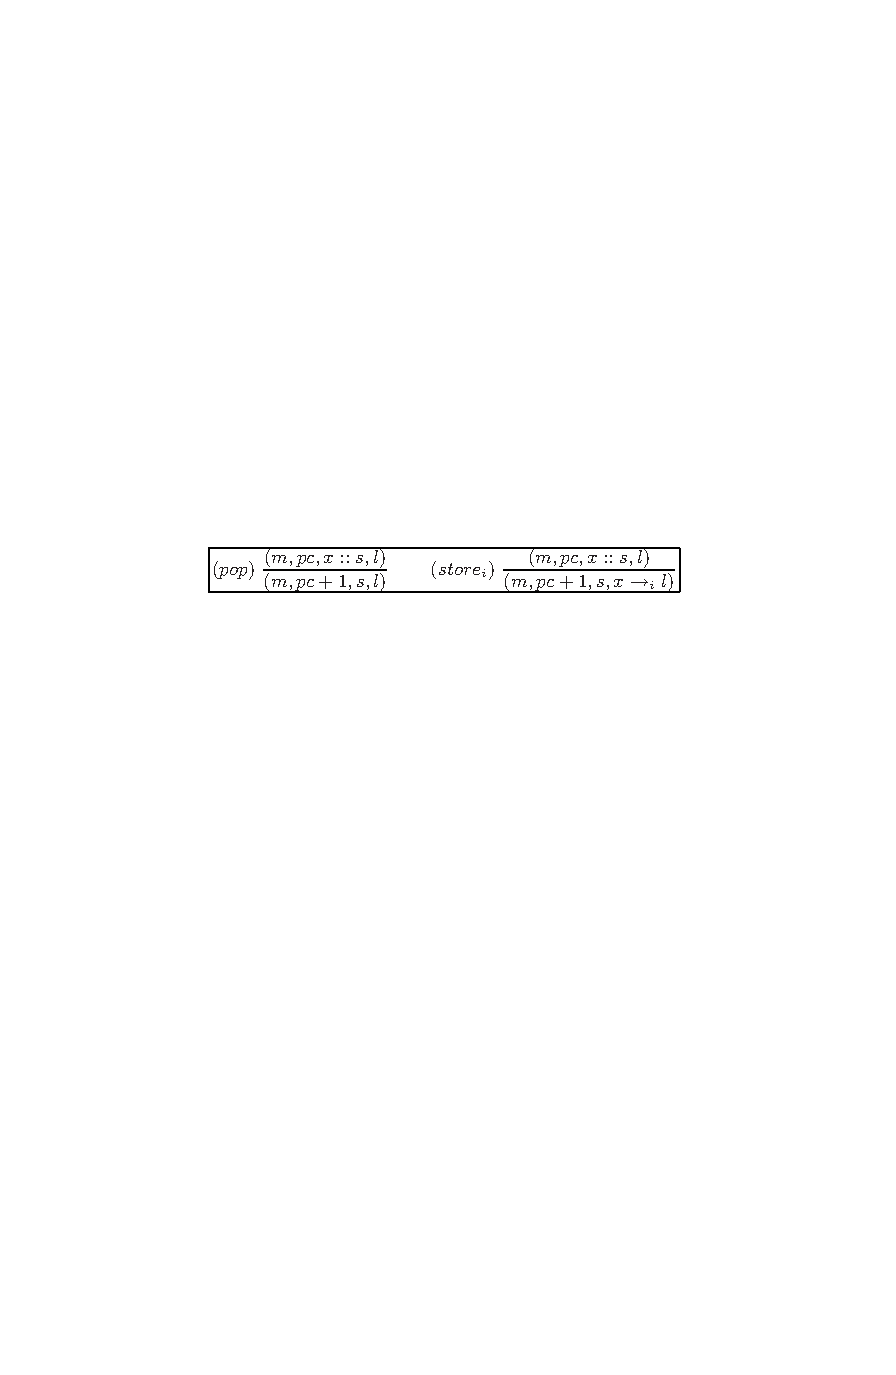
\includegraphics[scale=1.3]{jvm_1}
  \caption{\footnotesize Extrait de la sémantique opérationnelle du bytecode Java}
  \label{fig:semantique-java}
\end{figure}

On peut noter qu'en fonction de la nature des instructions, les règles
de la sémantique n'ont d'impact que sur une partie de l'état de la
machine virtuelle. Ainsi, la majorité des instructions ($\kw{store_i}$,
$\kw{aload\_0}$, $\kw{goto}$, $\kw{if\_icmpe}$, \dots) du ByteCode,
ne portent que sur le contexte de la méthode courante et/ou sur le tas
($\kw{get\_field}$, $\kw{put\_field}$. Cependant, les instructions
dédiées aux appels et retour de méthodes ($\kw{invokeVirtual}$, $\kw{return}$, \dots)
modifient la pile d'appel en plus du contexte de la méthode courante et
concerne une plus grande partie de l'état de la machine virtuelle.

Le système de réécriture généré par \emph{Copster} pour un programme
donné assure un certain nombre de bonnes propriétés issues de la
sémantique. Principalement, le système de réécriture produit est toujours
linéaire à gauche, déterministe, et préserve la séquentialité
des instructions de telle sorte qu'il n'existe qu'une seule manière de
réécrire chaque terme atteignable.  Le comportement de chaque
instruction est simulé par un ensemble de règles équivalent à la règle
sémantique. On peut voir dans la figure~\ref{fig:semantique-trs} qu'il suffit
de trois règles pour exécuter l'instruction au point de programme $pc_1$ de la méthode
$\kw{C.m1()}$. La règle (2) est la simple traduction de la règle sémantique de $\kw{pop}$,
alors que les règles (1) et (3) sont dédiées à la méthode $\kw{C.m1}()$, et donc propres au 
programme. La règle (1) permet de lier au point de programme $pc_1$ de $\kw{C.m1}()$ l'instruction
correspondante : $\kw{pop}$. On voit que la règle (1) convertit le contexte en un contexte intermédiaire $xframe(\dots)$
surlequel est défini la sémantique des instructions. Une fois l'exécution terminée, un nouveau 
contexte $frame(\dots)$ est produit. La règle (3) incrémente simplement l'index de l'instruction à exécuter.

\begin{figure}[ht!]
  \centering
  \[
  {%\footnotesize
    \begin{array}{|c|ll|}
      \hline
      1 & frame(name(m1, C), pc1, st, lv, h) & \lrw xframe(pop, name(m1, C), pc_1, st, lv, h)\\
      2 & xframe(pop, m, pc, stack(x, s), l, h) & \lrw frame(m, next(pc), s, l, h) \\
      3 & next(pc_1) &\lrw pc_2 \\
      \hline
    \end{array}
  }
  \]
  \caption{\footnotesize Règles pour l'instruction $\kw{pop}$ de la méthode $\kw{C.m1()}$}
  \label{fig:semantique-trs}
\end{figure}


Un point crucial pour la suite est la possibilité de déterminer une
classification des règles. En effet, la position à laquelle peut
réécrire une règle de réécriture dans un terme détermine la nature
sémantique de la règle. En se focalisant sur une position donnée du
terme, on peut alors analyser les séquences de réécriture
correspondant aux graphes d'appels des méthodes Java, les opérations
réalisées sur le tas \textit{etc}\dots\ On va donc montrer comment
exploiter cette propriété du langage pour réaliser une analyse
inter-procédurale du flot de contrôle pour des programmes Java.

\subsection{Chaîne de réécriture à la position $p$}

On considère $\R$ le système de règles de réécriture, et un ensemble d'équations $E$.
On va définir $\arw_{\R_p/E}$ une sous relation de $\rw_\RE^*$ la
relation de réécriture induite par $\RE$.  Le but de la relation
$\arw_{\R_p/E}$ est de caractériser la réécriture uniquement par les
étapes de réécriture qui ont lieu à la position $p$.

\begin{definition}
  \label{def:arw}
  Soient $s,\ t \in \TF$ deux termes tels que $s \rw_\RE^* t$.
  Soit $p \in \pos(s)$ une position de $s$. Alors on a \textbf{$s \arw_{\R_p/E} t$} si et seulement si
  il existe un terme $w$ qui satisfait les conditions suivantes:
  \begin{itemize}
  \item  $s \rw_\RE^* w$
  \item $w$ doit être obtenu par réécriture uniquement de sous-termes stricts de $s|_p$.
  \item $t=_E w[r\sigma]_p$ avec $l\rw r \in \R$ et $w|_p = l\sigma$
  \end{itemize}
\end{definition}

Dans le cas où l'ensemble des équations est vide, on note par $\arw_{\R_p}$ la relation $\arw_{\R_p/\emptyset}$.
De la même manière on utilise la notation $\arw_\RE$ pour $p = \epsilon$. Ce qui nous donne au final, la notation
$\arw_\R$ dans le cas $p = \epsilon$ et $E = \emptyset$.
On voit par l'intermédiaire de l'exemple~\ref{ex:arw}, que la relation $\arw_{\R_p}$ permet 
d'abstraire la séquence de réécriture: les différents étapes de réécriture nécessaires
pour arriver à l'étape de réécriture à la position $p$ sont simplement oubliées.
De ce fait, on ne conserve que les termes qui sont produits par la réécriture à la position $p$.
\begin{example}
  \label{ex:arw}
  On considère la séquence de réécriture suivante. A chaque étape, le
  sous-terme réécrit est souligné, et le sous-terme produit est en
  gras.
  \begin{multline*}
    f(g(\underline{a}), h(b)) \lrw_\R 
    f(\underline{g(\textbf{b})}, h(b)) \lrw_\R 
    f(\textbf{h(\underline{b})}, h(b)) \lrw_\R
    \\
    \\
    f(\textbf{a}, h(\underline{b})) \lrw_\R 
    f(a, \underline{h(\textbf{c})}) \lrw_\R 
    \underline{f(a, \textbf{a})} \lrw_\R 
    \textbf{g(f(a, a))} %\rw_\R 
    % \textbf{f(a, f(a, \underline{a})}) \rw_\R  %doit remplacer celle du dessus
    % f(a, f(a, \textbf{b}))
  \end{multline*}
  conformément à la définition~\ref{def:arw} on peut exhiber les relations suivantes:
  
  \medskip
  \begin{itemize}
  \item $f(g(a), h(b)) \arw_{\R_1} f(h(b), h(b))$
  \item $f(a, h(b)) \arw_{\R_2} f(a, a)$
  \item $f(g(a), h(b)) \arw_\R g(f(a,a))$
  \end{itemize}
\end{example}

Dans le cas où le système de réécriture modélise l'exéction d'un programme Java, la position de réécriture
permet de caractériser la nature sémantique l'étape de réécriture.
Si l'on considère $s$ un état conforme à la figure~\ref{fig:etat-terme} aux positions suivantes, on peut considérer:

\begin{itemize}
\item Le sous-terme $s|_1 = \la m_0, pc_0, \dots \ra$ est le contexte
  de la méthode en cours. La réécriture à la position $1$ correspond au début de
  l'exécution des instructions du byteCode.

\item La réécriture aux positions $s|_{13}$ et $s|_{14}$ correspond
  aux opérations élémentaires comme la modification de la pile ou des
  variables locales\dots
  
\item Plus intéressant, le sous-terme~$s|_{15}$ correspond au tas: les
  règles de réécriture appliquées à cette position concerne la
  consultation, la création ou la modification des objets ou tableaux
  stockés en mémoire.

\item Le sous-terme $s|_\epsilon$ soit $s$ lui-même, est réécrit par les
  règles qui correspondent aux appels et retours de méthodes.
\item \dots
\end{itemize}

On considère maintenant un état de la machine virtuelle correspondant
au début de l'exécution d'une méthode $m$ donné par le contexte $f_0 =
\la m, pc_0, \epsilon, lv_0, h_0\ra$, une certaine pile d'appels $fs$
et des entrées-sorties de la forme $I/O(\dots)$.  Cet état est la
forme $s_0 = state(f_0, fs, I/O(\dots))$. Si on déroule l'exécution de
la méthode pas-à-pas de l'instruction $\kw{instr}_i$ au point de
programme $pc_i$ on obtient un nouveau contexte $f_{i+1}$ par
réécriture. L'exécution de l'instruction débute par la réécriture de
l'état $s_i$ à la position $1$, ce qui construit un état intermédiaire, sur
lequel a lieu toutes les étapes de réécriture nécessaires pour
réaliser les différentes manipulations (sur les variables, la pile, le
tas) induites par l'exécution de l'instruction $\kw{instr}_i$. Comme
indiqué ci-dessus, ces étapes de réécriture ont lieu uniquement sur
les sous-termes de $f_i$: %situés aux positions $1[1..9]^*$:

\[ state(\underline{f_i}, fs, I/O(\dots)) \lrw_\R^* state(\mathbf{f_{i+1}}, fs, I/O(\dots)) \]

Si le point de programme $p_n$ correspond à un appel de la méthode
$m'$ qui va produire un nouvel état de la forme $state(f'_0, fs',
I/O(\dots))$ où le contexte est de la forme $f'_0 = \la m', pc_0,
\epsilon, lv'_0, h_n \ra$ et la pile $fs' = fstack((m, pc_n, st_n,
lv_n), fs)$. Au final, on obtient la séquence de réécriture suivante:
\begin{multline*}
  state(\underline{f_0}, fs, I/O(\dots)) \lrw_\R^* \underline{state(\mathbf{f_n}, fs, I/O(\dots))} \\
  \lrw_\R \mathbf{state(f'_0, fstack((m, pc_n, st_n, lv_n), fs), I/O(\dots))}  
\end{multline*}

\noindent qui peut être abstraite:
\[ state(f_0, fs, I/O(\dots)) \quad \arw_\R \quad state(f'_0, fstack((m, pc_n, st_n, lv_n), fs), I/O(\dots)) \]
Puisque $f_0$ et $f'_0$ représentent respectivement les états au point d'entrée des méthodes $m$ et $m'$, la relation ci-dessus
dénote bien à l'appel de la méthode $m'$ par $m$. Ainsi, les traces d'exécutions abstraites par la relation $\arw_\R$
permettent de construire le graphe d'appels d'un programme Java.
Ce graphe interprocédural peut-être obtenu par la complétion d'un automate d'arbres.
En fait l'automate étant souvent obtenu par une sur-approximation paramétrée par $E$ un ensemble d'équations, il caractérise 
un sous-ensemble de la relation plus générale $\arw_{\R_p/E}$. 

\section{Completion d'automates d'arbres et $\arw_{\R_p/E}$}

La relation $\arw_{\R_p/E}$ que l'on cherche à caractériser est en fait construite
et maintenue naturellement par la complétion. Elle est intrinsèquement liée à la nature
des automates d'arbres et finalement à la manière dont sont ajoutées les  $\varepsilon$-transitions 
par les étapes de complétion. En effet, chaque $\varepsilon$-transition de la forme $q' \rw q$
met en relation les représentants de $q'$ et $q$ par $\arw_{\R_\epsilon/E}$.
Ce qui nous donne la propriété suivante~:

\begin{lemma}
  \label{lem:completion_arw}
  Soit $\A = \la \F, \Q, \Q_f, \Delta \cup \Deps\ra$ un automate obtenu 
  par complétion à partir des règles $\R$ et des équations $E$.
  Alors pour toute transition $q' \lrw q \in \Deps$ de $\A$,
  et tous les représentants de $q$ et $q'$:
  \[
  \xymatrix{
    u \ar[dd]_{\A}^{\not\varepsilon} \ar@{-->} [rr]_{\R/E} && v \ar[dd]^{\A}_{\not\varepsilon}\\
    &&\\
    q && q' \ar[ll]
  }
  \]
  
  \end{lemma}

\begin{proof}
  La preuve se base sur la définition~\ref{def:re-coherence} de la $\RE$-cohérence qui est plus forte.
  Elle assure que pour tout état $q$ d'un automate produit par complétion, si $s \in \Rep (q)$ un représentant de l'état $q$
  alors~:
  \begin{itemize}
  \item $\forall t \in \Rep(q)$, $s =_E t$
  \item $\forall t \in \Lang(\A, q)$, $s \rw_\RE^* t$.
  \end{itemize}

  On considère la transition $q \rw q' \in \Deps$. Par construction, cette $\varepsilon$-transition est ajoutée
  par la résolution de la paire critique $\la q, r\sigma\ra$ formée par l'automate avec une règle $l\rw r \in \R$.
  On rappelle que la substitution $\sigma$ associe à chaque variable $x$ du membre gauche $l$ un état $\sigma(x) \in \Q$
  telle que:
  \[
  \xymatrix{
    l\sigma \ar[dd]^{\A}_{*} \ar[rr]_{\R}  & & r\sigma\\ % \ar[dd]^{\aaexeq^{k+1}}_{\not\varepsilon}\\
    & & \\
    q & &% q' \ar[ll]^{\aaexeq^{k+1}}
  }
  \]
  Une telle paire critique a été résolue en ajoutant à l'automate les transitions $r\sigma \rwne q'$ et $q' \rw q$.
  Ensuite on considère la subsitution $\sigma' : \X \rw \TF$ de la forme
  $\{ x \mapsto \sigma'(x) \sep \sigma'(x) \in \Rep(\sigma(x)) \}$. On a automatiquement $l\sigma' \rw_{\A}^* l\sigma$ :
  l'ensemble des substitutions $\sigma'$ dénotent les termes $l\sigma'$ reconnus en $q$ qui sont réécrits par la règle $l \rw r$ 
  tels que  $r\sigma'$ est un représentant de $q'$ puisque l'on a $r\sigma' \rwne_{\A} r\sigma$.

  Grâce au premier point de la définition~\ref{def:re-coherence} et la résolution de la paire critique
  on obtient le diagramme suivant:
  \[
  \xymatrix{
    u \ar[rr]_{\RE^*} \ar@/_2pc/[rrdd]^{\not\varepsilon}_{\A} & & l\sigma' \ar[dd]^{\A}_{*} \ar[rr]_{\R}  & & r\sigma' \ar[dd]^{\A}_{\not\varepsilon}\\
    & & & & \\
    & & q & & q' \ar[ll]^{\A}
  }
  \]
  où $u$ est un terme représentant quelconque de $q$. On obtient donc une chaîne de réécriture entre les termes $u$ et $r\sigma'$
  dont la dernière étape de réécriture est réalisée à la position $\epsilon$. De plus, 
  $u$ et $r\sigma'$ sont respectivement des représentants de états $q$ et $q'$.

  Pour établir la relation $u \arw_\RE r\sigma'$, il
  suffit de montrer qu'il n'y a aucune étape de réécriture située à la
  position $\epsilon$ sur $u \rw_\RE^* l\sigma'$.  Pour cela, il faut
  regarder une caractéristique de l'algorithme de filtrage: si
  $\sigma$ est une solution du problème de filtrage $l \match q$,
  alors on sait que $l\sigma \rw_\A^* q$.  Cependant, pour des raisons
  d'optimalité, la dernière transition utilisée pour réécrire
  $l\sigma$ en $q$, est une transition normalisée de $\Delta$, donc de
  la forme $f(q_1,\dots, q_n) \rw q$.  Il est suffisant de considérer
  ce cas pour que la paire critique soit aussi résolue pour tous les
  états dans lesquels $q$ peut-être réécrit: avoir $r\sigma \rw_\A^*
  q$ est suffisant pour obtenir la transition $r\sigma \rw_{\A}^* q''$
  pour toute paire critique $\la l\sigma, q'' \ra$ avec $q \rw_{\A}^*
  q''$ à partir d'une transition de la forme $l\sigma \rw^*_{\A} q
  \rw^*_\A q''$.
  
  On peut donc en déduire que tout terme $l\sigma'$ est un terme de la forme $f(t_1, \dots, t_n)$ tels que 
  pour chaque sous-terme on ait $t_i \rw_\A^* q_i$. D'après le premier point de la $\RE$-cohérence,
  on peut construire un terme $s_i$ représentant de $q_i$ tel que $s_i \rw_\RE^* t_i$. 
  Par composition, $f(s_1, \dots, s_n)$ est un représentant de l'état $q$:
  on a $ f(s_1,\dots, s_n) \rwne_\A f(q_1,\dots, q_n)$ et $f(q_1,\dots, q_n) \rw q \in \Delta$.
  On peut produire le terme $l\sigma'$ par réécriture des sous-termes stricts de $f(s_1, \dots, s_n)$.

  De plus, comme le terme $u$, le terme $f(s_1, \dots, s_n)$ est un représentant de $q$. En adéquation
  avec le second point de la $\RE$-cohérence, on peut en déduire que $u =_E f(s_1, \dots, s_n)$.
  De même $r\sigma'$ est un représentant de $q'$: donc pour tout représentant $v$ de $q'$ on a $r\sigma' =_E v$
  Finalement, cela permet de conclure la preuve puisqu'on a $u \rw_\RE^* l\sigma' \rw_\R r\sigma' =_E v$
  avec $l\sigma'$ obtenu uniquement par des étapes de réécriture sur des sous-termes stricts:

  \[
  \xymatrix{
    &&&&&\\
    u \ar@/_2pc/[rrdd]^{\not\varepsilon}_{\A} \ar[rr]_{\RE}^{*} \ar @/^1.8pc/ @{-->} [rrrrrr]^{\RE} &&
    l\sigma' \ar[dd]^{\A}_{*} \ar[rr]_{\R}&&
    r\sigma' \ar[dd]^{\A}_{\not\varepsilon} && v \ar@{=}[ll]^{E} \ar@/^2pc/[lldd]_{\not\varepsilon}^{\A}\\
    &&&&&\\
    && q && q' \ar[ll]^{\A} &
  }
  \]
  \noindent
  pour tout $u \in \Rep(q)$ et $v \in \Rep(q')$.
\end{proof}


\newcommand{\wrsav}{\wr}
\renewcommand{\wr}{\leftarrow}
  De cette propriété découle immédiatement la généralisation pour n'importe quelle position.
  En effet, on considère un terme $t \in \Lang(\A, q)$ tel que $t_p \in \Rep(q_1)$ et $t[q_1]_p \rw_\A^* q$:
  pour toute transition $q_2 \rw q_1\in \Deps$ alors pour tout $u_1 \in \Rep(q_1)$ on a $t \arw_{\R_p/E} t[u_1]_p$.
  Ainsi à partir de la chaîne de $\varepsilon$-transitions $q_1 \wr q_2 \wr q_3 \wr q_4 \wr \dots$,
  on peut déduire la séquence
  \[t \arw_{\R_p/E} t[u_1]_p \arw_{\R_p/E} t[u_2]_p \arw_{\R_p/E} t[u_3]_p \arw_{\R_p/E} t[u_4]_p \quad \dots\]
  \noindent avec $u_i \in \Rep(q_i)$.
\renewcommand{\wr}{\wrsav}


% The verification technique used in~\cite{BoichutGJL-RTA07}, called Tree Automata
% Completion~\cite{FeuilladeGVTT-JAR04}, is abble to finitely over-approximate the
% set of reachable terms, i.e. the set of all reachable states of the
% JVM. However, this technique lacks precision in the sense that it makes no
% difference between all those reachable terms. Due to the approximation
% algorithm, all reachable terms are considered as equivalent and the execution
% ordering is lost. This prevents, in particular, to prove temporal properties on such models. 
% However, using approximations make it possible to prove unreachability
% properties on infinite state systems.

% In this preliminary work, we propose to improve the Tree Automata Completion
% method so as to prove temporal properties on TRS representing a finite state
% system. The first step is to refine the algorithm so as to produce a tree
% automaton keeping an approximation of the rewriting relation between
% terms. Then, in a second step, we propose a way to check LTL-like formulas on
% this tree automaton.


\section{Extraction d'une structure de Kripke}
Soit $\aaexeq^*= \la \T(\F), \Q, \Q_F, \Delta \cup \Deps \ra$ un automate d'arbres obtenu par 
complétion pour $\R$ un système de réécriture donné, avec un ensemble d'équation $E$, à partir 
du langage initial~$I$. On suppose que $\aaexeq^*$ est $\R$-clos soit $\aaexeq^* \supseteq \R(\aaexeq^*)$.

Une structure de Kripke est un graphe orienté utilisé dans le model-checking pour représenter le comportement d'un système. 
Les noeuds représentent les états accessibles du système et les arcs représentent les transitions du système.
Une fonction d'étiquetage associe à chaque état l'ensemble des propriétés de cet état. 

\begin{definition}
Une structure de Kripke est un quadruplet de la forme $\K = (S, S_0, R, L)$ tel que
\begin{itemize}
\item $S$ est un ensemble d'états,
\item $S_0 \subseteq S$ est l'ensemble des états initiaux,
\item $R \subseteq S \times S$ est la relation de transition qui doit être totale à gauche,
\item $L$ est une fonction qui étiquette chaque état $s$ avec un ensemble de prédicats qui sont vrais 
  dans l'état $s$.
\end{itemize}
\end{definition}

On veut construire un tel modèle pour le sous-ensemble de la relation $\arw_{\R_p/E}$ contenu par l'automate $\aaexeq^*$
à partir d'un ensemble de termes $t_0 \in \Lang(\aaexeq^*)$. Cependant à cause du lemme~\ref{lem:completion_arw}, les sous-termes
initiaux $t_0|_p$  concernés par $\arw_{\R_p/E}$ doivent être des représentants de l'états qui les accepte :
\begin{equation*}
  \label{eq:1}
  t_0 \rwne_{\aaexeq^*} t_0[q]_p \rw_{\aaexeq^*}^* q_f,\quad \textrm{ avec } q_f \in \Q_f
\end{equation*}

On peut alors ramener le problème d'analyse de $\arw_{\R_p/E}$ à l'analyse de $\arw_{\R_p/E}$ pour les sous-termes $t_0|_p$.
Ces sous-termes sont des représentants pour l'état $q$, et l'acceptation de $t_0|_p$ par l'état $q$ est une étape dans la
reconnaissance de $t_0$ par l'automate. On note $Q_0$ l'ensemble de ces états $q$.

Pour construire le modèle de Kripke, on prend les états de l'automate comme états de la structure de Kripke, 
la fonction de transition $R$ est définie au moyen des $\varepsilon$-transitions.
Enfin l'ensemble des prédicats attachés à  chaque état est défini par l'ensemble des représentants associés à l'état. 
On définit alors la fonction de \textit{labelling} $L$ simplement par une fonction qui associe un automate d'arbres à chaque état.

\begin{definition}
  On définit la fonction de labelling $L : q \mapsto \la \F, \Q, \{q\}, \Delta\ra$ comme la fonction
  qui associe à un état $q$, l'automate $L(q)$ issu de l'automate $\aaexeq^*$ privé des $\varepsilon$-transitions
  et pour lequel $q$ est l'unique état final.
  Par construction, on peut montrer que les termes reconnus par l'automate $L(p)$ sont exactement les représentants
  de l'états $q$ dans l'automate complet $\aaexeq^*$.
  \[\forall t \in \Lang(L(q)), \quad t \rwne_{\aaexeq^*} q\]
\end{definition}

Ce qui permet alors de construire la structure de Kripke correspondant à la relation $\arw_{\R_p/E}$ pour l'ensemble des termes $t_0$.

\begin{definition}%[Construction of a Kripke Structure]
  On construit le quadruplet $(S, S_0, R, L)$ à partir de l'automate $\aaexeq^*$.
  Chaque composante du quadruplet se définit par:
  \begin{itemize}
  \item $S = \Q$, 
  \item $S_0 = Q_0$,
  \item $R(q, q')$ si $q' \rw q \in \Deps$
  \item la fonction de labelling $L$ telle que définie ci-dessus.
  \end{itemize}
\end{definition}

Cependant, une structure de Kripke doit être constituée d'une relation $R$ qui soit totale à gauche.
Ainsi pour n'importe quel état $q$ qui n'a pas de successeur par $R$, on le fait boucler sur lui-même
de façon à avoir $R(q, q)$. Cette transformation relativement classique provient du fait que
la logique temporelle CTL$^*$ utilisée pour formaliser les propriétés reposent sur des modèles dont les traces
d'exécution sont infinies.

Dans notre analyse inter-procédurale, ce sont les étapes de réécriture au sommet des termes qui caractérisent
les appels et retours de méthodes dans les programmes Java. En supposant que l'ensemble des états finals de $\aaexeq^*$ est $\Q_f$,
on veut donc obtenir un modèle pour la relation de transition induite par la relation $\arw_{\R/E}$, pour les termes $t_0 \in I$ l'ensemble initial. Ce qui implique
que l'ensemble des états initiaux $S_0$ correspond simplement à $\Q_f$, l'ensemble des états finals de 
l'automate. En effet, tout terme initial de $I$ est systématiquement un représentant d'un état final par construction.

% Une structure de Kripke est paramétrée par l'ensemble $S_0$.
% It defines which connected component of $R$ we are interested to analyze. For instance, to analyze 
% the abstract rewriting at the top position of terms in $\Lang{}(\aaex^*)$, we define
% set $S_0 = \Q_F$ (the set of final states of $\aaex^*$), since all canonical
% terms of final states are initial terms. 
% For all abstract rewriting at a deeper position $p$, we need to define 
% a set $Sub$ of initial subterms considered as the beginning of the rewriting
% at the position $p$. Then the set $S_0$ will be defined as 
% $S_0 = \{q \sep \exists t \in Sub,\; t \rwne_{\aaex^*} q\}$.
 
La structure de Kripke obtenue modélise la relation de réécriture $\arw_\RE^*$ 
à la position $p$ à partir des sous-termes $t_0|_p$.

\begin{theorem}
  Soit $\K=(S, S_0, R, L)$ la structure de Kripke extraite à partir de l'automate $\aaexeq^*$.
  Pour tous les états $s$, $s'$ tels que $R(s, s')$ soit vraie, alors pour tous les termes
  $u \in \Lang(L(s))$ et $v \in \Lang(L(s'))$ on a  $u \arw_{\RE} v$. De plus, pour tout terme $u,\ v \in \Lang(L(s))$
  de tout état $s$, on a $u =_E v$.
\end{theorem}

\begin{proof}
  Ce théoréme est la conséquence immédiate du lemme~\ref{lem:completion_arw} 
  appliqué à l'automate $\aaexeq^*$ et de la définition de la relation de transition $R$.
\end{proof}



\begin{example}
  \label{the_example}
  Pour illustrer ce résultat, on propose de considérer l'automate d'arbres suivant obtenu par complétion
  à partir du système de réécriture $\R$ défini par $\{ a \rw b,\; b\rw c \} \cup \{f(c) \rw g(a),\; g(c) \rw h(a),\; h(c) \rw f(a)\}$.
  On part de l'ensemble initial $I=\{f(a)\}$.
  Sans approximation, \textit{i.e.} $E = \emptyset$, on obtient l'automate point fixe suivant~:
  {\small
    \[\aaex^*= \left\la
      \Qf = \{q_f\},\quad
      \Delta = \left\{
        \begin{array}{rcl}
          a & \rw & q_a \\
          b & \rw & q_b \\
          c & \rw & q_c \\
          f(q_a) & \rw & q_f \\
          g(q_a) & \rw & q_g \\
          h(q_a) & \rw & q_h \\
        \end{array}
      \right\}\:
      \Deps= \left\{
        \begin{array}{rcl}
          q_b & \rw & q_a \\
          q_c & \rw & q_b \\
          q_g & \rw & q_f \\
          % q_f & \rw & q_g \\
          q_h & \rw & q_g \\
          q_f & \rw & q_h \\
        \end{array}\right\}
      \:
    \right\ra
    \]
  }
  
  \noindent Si on regarde la transition $q_h \rw q_g$, et les termes $h(a)$ et $g(a)$ représentants de $q_h$ et $q_g$ respectivement, 
  on en déduit $g(a) \arw_\R h(a)$. Ce qui correspond bien à
  $g(\underline{a}) \rw_\R g(\underline{\textbf{b}}) \rw_\R \underline{g(\textbf{c})} \rw_\R \textbf{h(a)}$.
%   Dans l'exemple~\ref{the_example}, si on veut vérifier une propriété sur $\arw_\R$
%   on a besoin de seulement considérer sous-ensemble de transitions de $\Deps$ qui correspondent 
%   à l'abstraction de la relation de réécriture $\arw_\R$.
%%%%%   The subsets are quite simple 
  Les figures~\ref{fig2}~et~\ref{fig3} montrent l'extraction de la structure de Kripke à partir de l'automate
  pour les relation $\arw_{\R_1}$ et$\arw_{\R_\epsilon}$ respectivement.
  % Note that in figure~\ref{fig2}, a loop is needed on state $c$ to have a total relation
  % for $\K_1$.
  
  \begin{figure}[!ht]
    \begin{minipage}{0.5\linewidth}
      \centering
      \begin{tikzpicture}[thick, initial text=]
        \tikzstyle{every node}=[font=\tiny]
        \tikzstyle{every state}=[minimum size=.8cm]
        \tikzstyle{accepting}=[accepting by double]
        \node [initial,state] (a) at (0, 0) {$q_a$}; 
        \node [state] (b) at (2, 0) {$q_b$};
        \node [state] (c) at (4, 0) {$q_c$};
        \node [] (f) at (0, 1.8) {};
        \draw[->] (a) edge (b) (b) edge (c) (c) [loop right] edge (c);
      \end{tikzpicture}
      % 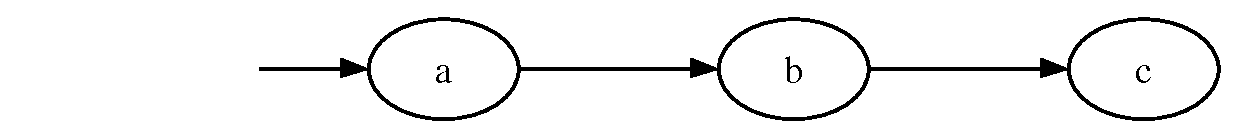
\includegraphics[scale=0.4]{R1}
      \caption{\label{fig2}\footnotesize $\K_1$ modélise $\arw_{\R_1}$}
    \end{minipage}
    \begin{minipage}{0.5\linewidth}
      \begin{center}
        \begin{tikzpicture}[thick, initial text=]
          \tikzstyle{every node}=[font=\tiny]
          \tikzstyle{every state}=[minimum size=.1cm]
          \tikzstyle{accepting}=[accepting by double]
          \node [initial,state] (a) at (0, 0) {$q_f$}; %{$f(a)$}; 
          \node [state] (b) at (2, 0) {$q_g$}; %{$g(a)$};
          \node [state] (c) at (1, 1.5) {$q_h$}; %{$h(a)$};
          \draw[->] (a) edge (b) (b) edge (c) (c) edge (a);
        \end{tikzpicture}
        % 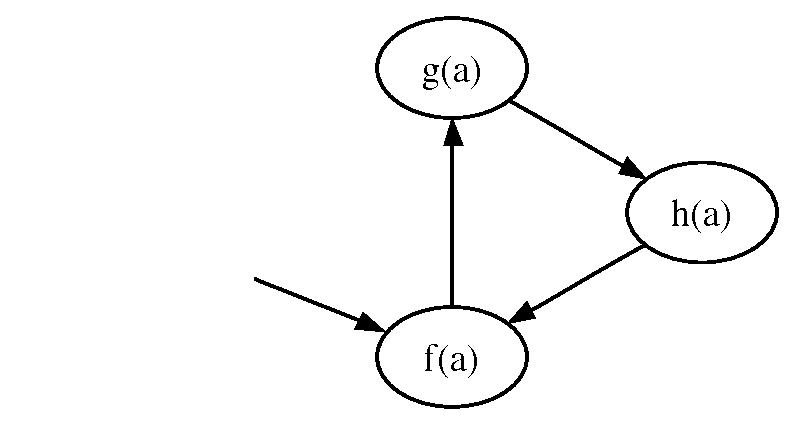
\includegraphics[scale=0.4]{R2}
        \caption{\label{fig3}\footnotesize $\K_\epsilon$ modélise $\arw_{\R_\epsilon}$}
      \end{center}
    \end{minipage}
  \end{figure}
\end{example}


% \comments{REFAIRE LES SCHEMAS : REMPLACER LES TERMES PAR DES ETATS CORRESPONDANTS
% OU ETATS (TERMES)? Moi je laisserais les termes sur cet exemple car ca permet de
% comprendre mieux ou on va. Quite a mettre les etats dans la suite de l'exemple
% et expliquer qu'ils reconnaissent ces termes.}

% The set $S_0$ of initial states depends of the abstract rewriting relation selected.
% For example, if we want to analyze $\arw_{\R_2}$ (or $\arw_{\R_1}$), we define $S_0=\{q_f\}$ (resp. 
% $S_0 = \{q_a\}$).

\section{Une logique temporelle portant des automates d'arbres}

A partir du moment où l'on obtenu un modèle de Kripke $\K = (S, S_0,
R, L)$, on a accès à l'ensemble des techniques exploitant ce type de
modèle~\cite{MC-Book}. la logique temporelle CTL$^*$ est une logique permettant
de raisonner sur les structures de Kripke, elle constitue donc la base des techniques
du model-checking. Cette logique est basée sur le dépliage des traces
d'exécution possibles à partir d'un état initial du modèle. Une trace
d'exécution est caractérisée par une séquence infinie d'états de la
forme $\pi = s_0, s_1, s_2, \dots$ telle que $(s_i, s_{i+1}) \in
R$. On utilise les notations $\pi(i)$ et $\pi^i$ pour dénoter respectivement
le $i^\text{ème}$ état $s_i$ de $\pi$, et le suffixe de $\pi$ commençant à l'état $s_i$.
Dans la suite, on va s'intéresser à la logique temporelle linéraire LTL, sous-ensemble de CTL$^*$,
pour illustrer l'adaptation des techniques de vérifications sur les modèles extraits à partir 
des automates complétés.


\subsection{La logique LTL, et les automates d'arbres}

Une des particularité de cette approche est l'étiquetage des états du modèle par des automates d'arbres.
Initialement, la logique temporelle est définie sur les différents opérateurs logiques et temporels
($\land$, $\lor$, $\neg$, $\nxt$, $\fut$, $\gbl$, $\unt$, $\rel$) à partir de prédicats qui consituent 
les formules atomiques. Si la sémantique des différents opérateurs est préservée, on modifie celles des
formules atomiques représentées les prédicats étant alors représenté par des automates d'arbres.
On propose de définir le Regular Linear Temporal Logic (R-LTL). La R-LTL est la logique LTL où les prédicats sont définis par des
automates d'arbres. Le langage d'un tel automate d'arbres caractérise l'ensemble des termes qui sont admissibles pour le prédicat.

Ainsi un état $q$ d'une structre de Kripke $\K$ valide le prédicat $P$ caractérisé
par l'automate d'arbres  $\A_p$ si et seulement si un terme $t$ reconnu par l'automate
$L(q)$ satisfait le prédicat $P$. Cela implique que le terme $t$ soit lui aussi reconnu
par l'automate $\A_P$. Ce qui nous donne la nouvelle règle sémantique:
\[\K,\ q \models P\quad \equ\quad \Lang{}(L(q)) \cap \Lang{}(\A_P) \neq \emptyset\]

L'intuition est que le langage de l'automate $\A_p$ décrit une propriété par un ensemble de termes possibles.
On peut alors reformuler la satisfiabilité du prédicat $P$ pout $t$ par une disjonction de la forme 
$\bigvee_{u \in \Lang(A_p)} t = u$.
Cela représente un avantage notable pour exprimer des motifs réguliers sur les termes. En effet, il est facile 
de construire un automate qui décrit une propriété par tous les termes de la forme $f(a, f(x, y))$.
Quant à l'automate $L(q)$, il fournit l'ensemble des termes qui sont accessibles par $\arw_\RE$.
De ce fait, il est alors raisonnable de considérer que l'état $q$ satisfait le prédicat $P$ si l'un des termes reconnus par $L(q)$ est aussi
dans le langage de $A_p$, ce qui est équivalent à $\Lang{}(L(q)) \cap \Lang{}(\A_P) \neq \emptyset$.
\begin{figure}[ht!]
  \centering
  \[\begin{array}{|lcl|}
    \hline
    \K, s \models \neg f & \equ &  \K, s \not\models f\\
    \K, s \models f_1 \lor f_2 & \equ & \K, s \models f_1 \textrm{ ou } \K, s \models f_2\\
    \K, s \models f_1 \land f_2 & \equ & \K, s \models f_1 \textrm{ et } \K, s \models f_2\\
    &\dots&\\
    \hline
    \K, \pi \models f & \equ & \K, \pi(0) \models f\\
    \K, \pi \models \nxt g & \equ & \K, \pi^1 \models g\\
    \K, \pi \models \fut g & \equ & \exists k \ge 0,\ \K \pi^k \models g \\
    \K, \pi \models \gbl g & \equ & \forall i \ge 0,\ \K \pi^i \models g \\
    &\dots&\\
    \hline
  \end{array}\]
  \caption{Principaux connecteurs logiques de LTL}
  \label{fig:operateursLTL}
\end{figure}
La figure~\ref{fig:operateursLTL}, présente un sous-ensemble des
connecteurs logiques de LTL. On peut y distinguer deux types de
formules, celles comme $f$, $f_1$, $f_2$ qui portent sur les états
et les formules comme $g$ qui portent sur une séquence.  Dans le chapitre~3
de~\cite{MC-Book}, on trouve le détail de la sémantique de tous les
opérateurs, ainsi que les règles de construction des formules en LTL.


Les transitions de la structure $K$ dénotent les étapes de réécriture abstraite $\arw_{\RE}$
plutôt que sur la relation de réécriture $\rw_\RE$. Comme la sémantique des opérateurs est définie
sur la relation de transitions de $K$, les propriétés que l'on peut exprimer et vérifier portent bien
sur la relation $\arw_\RE$.
% Note that temporal properties do not range over the 
% rewriting relation $\rw_\R$ but over its abstraction $\arw_\R$.
% It means that the semantics of the temporal operators has to be interpreted
% w.r.t. this specific relation. 

Par exemple, la formule\footnote{\footnotesize Par soucis de simplicité dans les 
  petits exemples, plutôt que de représenter chaque prédicat par un automate, on représente directement 
  l'ensemble des termes que devrait accepter l'automate caractérisant le prédicat.}
  $\gbl(\{f(a)\} \imp \nxt \{g(a)\})$ sur $\K_\epsilon$ (\textit{c.f.} figure~\ref{fig3}) : la formule
doit être interprétée comme pour tout $q$ $q'$, si $\K_\epsilon,\ q \models \{f(a)\}$ et $R(q, q')$ alors
on a  $\K_\epsilon,\ q' \models \{g(a)\}$. D'un point de vue de la réécriture par~$\R$ (exemple~\ref{the_example}), le seul terme
$u$ tel que $f(a) \arw_{\R_\epsilon} u$ est $u = g(a)$.


\subsection{Les automates de Büchi}


Les propriétés en logique LTL peuvent être vérifiées au moyen de la théorie des automates de Büchi.
Les automates de Büchi~\cite{Buchi} sont des automates finis qui reconnaissent des mots de taille infinie. 
Les mots infinis vont permettre de représenter les comportements du modèle dont les traces d'exécution
sont infines. La structure des automates de Büchi est équivalente à celle des automates de mots finis.

\begin{definition}
  Un automate de Büchi se définit comme un quintuplet de la forme $\B = \la \Sigma, \Q, \Delta, \Q_0, \F\ra$
  avec
  \begin{itemize}
  \item $\Sigma$, un alphabet
  \item $\Q$, un ensemble d'états 
  \item $\Delta \subseteq \Q \times \Sigma \times \Q$, la relation de transition
  \item $\Q_0 \subseteq \Q$ et $\F \subseteq \Q$, les états initiaux et acceptants respectivement.
  \end{itemize}
\end{definition}
Un mot infini $w \in \Sigma^\omega$ est un mot qui contient un nombre
infini de répétitions\footnote{\footnotesize La répétition infinie est
  caractérisée par l'exposant $\omega$}. Il est accepté par un
automate de Büchi si et seulement si il existe une exécution infinie à
partir d'un état initial et qui passe infiniment souvent par un état
acceptant.

\begin{example}
  Exemple d'automate de Büchi:\\

%  \begin{tabular}{cp{10cm}}
 %   \begin{minipage}{5cm}
  \begin{center}
    \begin{tikzpicture}[scale=.8,thick,initial text=]
      \tikzstyle{every node}=[font=\tiny]
      \tikzstyle{every state}=[minimum size=.1cm]
      \tikzstyle{accepting}=[accepting by double]
      % 
      \node [initial,state] (q1) at (0, 0) {$1$}; 
      \node [accepting, state] (q2) at (4, 0) {$2$};
      % 
      \path[->]
      (q2)  edge [loop right] node {$b$} (q2) 
      edge [bend left] node [above] {$c$} (q1)
      (q1)  edge [bend left] node [above] {$a$} (q2);
    \end{tikzpicture}
  \end{center}
    % \end{minipage}
    % \hspace{1cm}
    % &
  L'automate ci-contre reconnaît le langage $\omega$-régulier $a(b^*ca)^\omega$,
  soit des mots infinis de la forme $acabbbbcabbca\dots$ par exemple.
  % \end{tabular}
\end{example}



Pour vérifier que le modèle $\K$ statisfait la propriété $P$ exprimée en R-LTL, 
il faut construire deux automates de Büchi $\B_\K$ et $\B_P$ qui acceptent respectivement
tous les comportements du modèle, et tous les comportements spécifiés par $P$.
La procédure de vérification revient alors à s'assurer que tous les comportements du modèle
$K$ sont couverts par la spécification $P$, ce qui se traduit par $\Lang(\B_\K) \subseteq \Lang(\B_P)$.
La manière standard de vérifier l'inclusion revient à vérifier qu'aucun comportement de
$\K$ ne viole $P$:
\[ \Lang(\B_\K) \cap \overline{\Lang(\B_P)} = \emptyset \]

Bien sûr, la vacuité du langage est décidable pour les automates de
Büchi, et ils sont clos par intersection et complémentation~\cite{Buchi}.

Il suffit de construire l'automate $\B_\K$ et l'automate $\overline{\B_P}$ qui reconnaît le langage $\overline{\Lang(\B_P)}$.
L'alphabet $\Sigma$ est constitué par les langages réguliers de termes de $\TF$ dénotés par les 
automates d'arbres.

\begin{definition}
  A partir du modèle $\K = (S, S_0, R, L)$, on définit l'automate de Büchi
  qui reconnaît tous les comportements de $\K$ comme $\B_\K =\la \Sigma, S \cup \{\iota\}, \Delta, \{\iota\}, S \cup \{\iota\}\ra$
  tel que $\Sigma = 2^\TF$, l'état initial est $\iota \not\in S$, et on a les transitions $(s, L(s'), s') \in \Delta$ si et seulement si $(s, s') \in R$.
  De plus, on ajoute à $\Delta$ les transitions $(\iota, L(s), s)$ pour tout état $s \in S_0$.
\end{definition}
Par construction tous les états de $\B_\K$ sont finals, pour permettre à tout chemin infini
de la structure de Kripke d'être un mot reconnu par $\B_\K$.
Si $\pi=s_0s_1s_2s_3\dots$ est une séquence valide d'états dans la structure de Kripke,
alors le mot $\pi' = L(s_0)L(s_1)L(s_2)\dots$ est reconnu par $\B_\K$.
Ce mot $\pi'$ dénote l'ensemble de séquence de réécriture de la forme
$t_0 \arw_\RE t_1 \arw_\RE t_2 \arw_\RE \dots$ tels que $t_i \in \Lang(L(s_i))$.

\begin{example}
  La figure~\ref{fig5} définit l'automate de Büchi qui pour la figure de Kripke $\K_\epsilon$:
  \begin{figure}[ht!]
    \begin{minipage}{0.5\linewidth}
      \begin{center}
        \begin{tikzpicture}[thick, initial text=]
          \tikzstyle{every node}=[font=\tiny]
          \tikzstyle{every state}=[minimum size=.1cm]
          \tikzstyle{accepting}=[accepting by double]
          \node [initial,state] (a) at (0, 0) {$q_f$}; %{$f(a)$}; 
          \node [state] (b) at (2, 0) {$q_g$}; %{$g(a)$};
          \node [state] (c) at (1, 1.5) {$q_h$}; %{$h(a)$};
          \draw[->] (a) edge (b) (b) edge (c) (c) edge (a);
        \end{tikzpicture}
        % 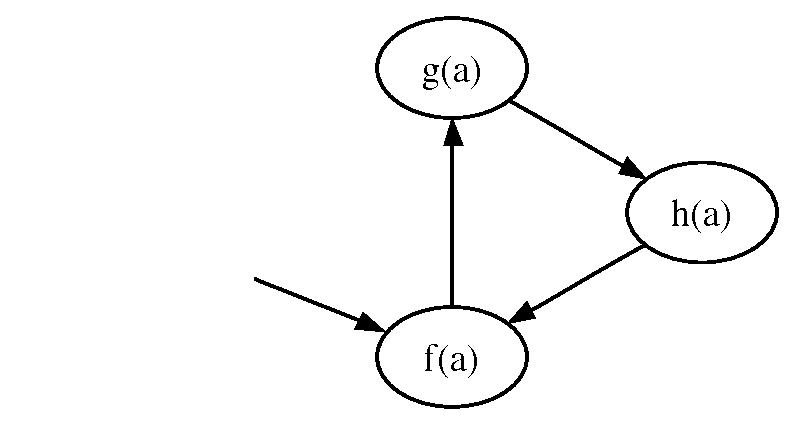
\includegraphics[scale=0.4]{R2}
      \end{center}
    \end{minipage}
    \begin{minipage}{0.5\linewidth}
      \begin{center}
        \begin{tikzpicture}[scale=.8,thick,initial text=]
          \tikzstyle{every node}=[node distance=40,font=\tiny]
          \tikzstyle{accepting}=[accepting by double]
          \tikzstyle{every state}=[accepting, minimum size=.1cm]
          % 
          \node [initial,state] (q4)            {$4$}; 
          \node [state] (q5) [right of=q4]      {$5$};
          \node [state] (q6) [below of=q5]      {$6$};
          \node [state] (q7) [right of=q6]      {$7$};
          % 
          \path[->]
          (q4)  edge []                         node [above]    {$L(q_f)$} (q5) 
          (q5)  edge []                         node [left]     {$L(q_g)$} (q6)
          (q6)  edge []                         node [below]    {$L(q_h)$} (q7)
          (q7)  edge [bend angle=40,bend right] node [right]    {$L(q_f)$} (q5);
        \end{tikzpicture}
      \end{center}
    \end{minipage}
    \caption{\footnotesize Construction l'automate $\B_{\K_\epsilon}$ pour le modèle $\K_\epsilon$}
    \label{fig5}
  \end{figure}
\end{example}

On ne s'étendra pas ici sur les techniques permettant de contruire l'automate de Büchi $\overline{\B_P}$ dénotant
la négation de la formule LTL $P$, mais il est possible de trouver les détails de l'algorithme pour construire ce type
d'automate dans~\cite{DBLP:conf/pstv/GerthPVW95}.
\begin{example}
  Soit la formule $P = \gbl(\{f(a)\} \imp \nxt \{g(a)\})$.
  L'automate $\overline{\B_P}$ (fig.~\ref{fig4}) reconnaît la négation de la formule $P$
  exprimée par $\fut(\{f(a)\} \land \nxt \neg\{g(a)\})$ et $\B_\K$ (fig.~\ref{fig5}) 
  reconnaît l'ensemble des comportements de la  structure de Kripke
  $\K_\epsilon$~(fig.~\ref{fig5}). La notation $\A_\alpha$ dénote l'automate d'arbres tel que son langage est décrit par $\alpha$
  ($\A_{\neg g(a)}$ reconnaît la complément du langage $\Lang{}(\A_{g(a)})$ et $\A_*$ reconnaît tout terme de $\TF$).
  \begin{figure}[ht!]
    \centering
    % \bar{\B_L}
    \begin{tikzpicture}[scale=.8,thick,initial text=]
      \tikzstyle{every node}=[font=\tiny]
      \tikzstyle{every state}=[minimum size=.1cm]
      \tikzstyle{accepting}=[accepting by double]
      % 
      \node [initial,state] (q1) at (0, 0) {$1$}; 
      \node [state] (q2) at (2, 0) {$2$};
      \node [accepting, state] (q3) at (4, 0) {$3$};
      % 
      \path[->]
      (q1)  edge [loop above] node {$\A_*$} (q1) 
      edge node [above] {$\A_{f(a)}$} (q2)
      (q2)  edge node [above] {$\overline{\A_{g(a)}}$} (q3)
      (q3)  edge [loop above] node {$\A_*$} (q3);
    \end{tikzpicture}
    \caption{\footnotesize l'automate $\overline{\B_P}$}
    \label{fig4}  
  \end{figure}
\end{example}

% For example, the formula $\gbl(\{f(a)\} \imp \nxt \{g(a)\})$
% on $\K_2$ (for more clarity, we note predicates as sets of terms): the formula 
% has to be interpreted as : for all $q$ $q'$, if $\K_2,\ q \models \{f(a)\}$ and $R(q, q')$ then
% we have  $\K_2,\ q' \models \{g(a)\}$. In the rewriting interpretation the only term $u$ such
% that $f(a) \arw_{\R_2} u$ is $u = g(a)$.

% On utilise les automates de Büchi pour réaliser la vérification de la propriété.
% La théorie des automates de Büchi et cette technique sont détaillées dans le chapitre~9
% de~\cite{MC-Book}. Comme les formules LTL, il est possible de traduire les formules R-LTL
% ainsi que la structure de Kripke en automates de Büchi.
% On construit alors deux automates de Büchi: $\B_\K$ obtainu obtenu à partir de la structure
% de Kripke et $\B_L$ défini par la formule R-LTL qui décrit la propriété.
% Comme l'ensemble des exécutions possible de la structure de Kripke est le langage accepté
% par l'automate $\B_\K$, la structure de Kripke satisfait la formule R-LTL si 
% toutes ses traces d'exécution sont reconnues par l'automate $\B_L$.
% Cela signifie qu'il faut vérifier $\Lang(\B_\K) \subseteq \Lang(\B_L)$. 
% Pour cela, l'approche standard consiste à construire l'automate $\overline{\B_L}$ 
% qui reconnaît l'ensemble des traces qui ne satisfont pas la formule $L$:
% ce qui corespond au langage $\overline{\Lang(\B_L)}$. Ensuite il suffit de 
% vérifier la vacuité de l'automate $\B_\cap$ qui reconnaît l'intersection des 
% langages $\Lang(\B_K)$ et $\overline{\Lang(\B_L)}$. Si cette intersection
% est vide, the term rewriting system satisfait la propriété.
% C'est l'application de la technique de model-checking standard.

% $\B_\M$ et $\B_\K$ sont classiquement définis comme des quintuplets: alphabet, états,
% états initiaux, états finaux et relation de transition.
% Généralement, l'alphabet d'un automate de  Büchi est un ensemble de prédicats.
% Puisqu'on utilise ici des automates d'arbres pour définir les prédicats, l'alphabet de
% $\B_\K$ et $\B_L$ est $\Sigma$ l'ensemble des automates d'arbres que l'on peut définir sur $\TF$. 
%  Les algorithmes
% utilisés pour construire $\B_\M$ et $\B_\K$ peuvent être trouvés dans~\cite{MC-Book}.


L'automate intersection $\B_\cap$ est obtenu en calculant le produit de automates $\B_\K$ et $\overline{\B_P}$.
Comme tous les états sont finals dans l'automate $\B_\K$, il est possible d'employer une version plus
simple du produit général d'automates de Büchi pour ce cas particulier~\cite{MC-Book}. On présente une version
adaptée de cet algorithme pour les automates de Büchi dont les transitions étiquetées par des automates d'arbres.

\begin{definition}[$\B_\K \times \overline{\B_P}$]
  Le produit de $\B_\K = \la \Sigma,\; \Q,\; Q_0,\; \Q,\ \Delta\ra$ par 
  $\overline{\B_P} = \la\Sigma,\; \Q',\;\Q'_0,\; \F',\ \Delta'\ra$ est défini
  \[\la \Sigma,\; \Q \times \Q',\; \Q_0 \times \Q'_0,\; \Q \times F',\; \Delta_\times\ra \]
  où $\Delta_\times$ est un ensemble de transitions $(q_\K, q_P) \xrw{(\A_\K\cap\A_P)} (q'_\K, q'_P)$ tel que $q_\K
  \xrw{\A_\K} q'_\K$ est une transition
  de $\B_\K$ et $q_P \xrw{\A_P} q'_P$ est une transition de $\overline{\B_P}$. De plus, la transition 
  est seulement valide si l'intersection entre les langages de $\A_\K$ et $\A_P$ est non vide.
  %comme attendu par la satisfiabilité d'une formule atomique en R-LTL.
  % as expected by the interpretation of the R-LTL atomic formula.
\end{definition}
L'intersection d'automates d'arbres calculée sur chaque transition de
l'automate intersection se justifie simplement.  Une transition de la forme
$s, A, s'$ pourrait être vue comme un ensemble de transitions de la
forme $s, t, s'$ où $t \in \Lang(A)$. Ainsi l'intersection placée sur
les transitions du produit $\B_\K \times \overline{\B_P}$ correspond
simplement à l'ensemble des transitions $((s_1, s_2), t, (s_1',s_2'))$
tel que $t \in \Lang(\B_\K)$ et $t \in \Lang(\B_P)$.

Enfin, la vacuité du langage $\Lang{}(\B_\cap)$ peut être vérifiée en utilisant l'algorithme
basé sur la recherche en profondeur qui assure que toute composante fortement connexe accessible à partir d'un état initial
ne contient pas d'états acceptants.


\begin{example}

  Pour illustrer l'approche, on propose de vérifier pour la formule $P
  = \gbl(\{f(a)\} \imp \nxt \{g(a)\})$ de l'exemple~\ref{the_example}.
  La figure~\ref{fig6} montre le résultat de l'intersection $\B_\cap$
  entre $\B_\K$ et $\overline{\B_P}$. Seul les états atteignables
  states et les transitions valides (étiquetées par une intersection
  non vide d'automates d'arbres) sont montrées.  Comme aucun état
  atteignable de $\B_\cap$ n'est final, sont langage est vide. Cela
  signifie que toutes les traces d'éxecution de $\K_\epsilon$
  satisfont $P$: en effet, le seul successeur de $f(a)$ pour
  $\arw_{\R_\epsilon}$ est $g(a)$.


\begin{figure}[ht!]
    % \bar{\B_\K}
  %\begin{minipage}{0.5\linewidth}
    \centering
    % B_\cap
    \vspace{10mm}
    \begin{tikzpicture}[scale=.8,thick,initial text=,bend angle=40]
      \tikzstyle{every node}=[node distance=50,font=\tiny]
      \tikzstyle{accepting}=[accepting by double]
      \tikzstyle{every state}=[minimum size=.1cm]
      % 
      \node [initial,state] (q14)            {$1,4$}; 
      \node [state] (q15) [right of=q14, node distance=60]     {$1,5$};
      \node [state] (q16) [below of=q15]     {$1,6$};
      \node [state] (q17) [right of=q16, node distance=60]     {$1,7$};
      \node [state] (q25) [below of=q14]     {$2,5$};
      % 
      \path[->]
      (q14) edge []                 node [above]           {$\A_* \cap L(q_f)$}       (q15)
            edge []                 node [left]            {$\A_{f(a)}\cap L(q_f)$}    (q25)
      (q15) edge []                 node [left]            {$\A_* \cap L(q_g)$}       (q16)
      (q16) edge []                 node [above]           {$\A_* \cap L(q_h)$}       (q17)
      (q17) edge [bend right]       node [right]           {$\A_* \cap L(q_f)$}       (q15)
            edge [bend left]        node [below]           {$\A_{f(a)} \cap L(q_g)$}   (q25);
    \end{tikzpicture}
    \caption{\footnotesize Automaton $\B_\cap$}
    \label{fig6}
%  \end{minipage}
\end{figure}
\end{example}




\section{Conclusion, discussion}

Dans ce chapitre, on a montré comment
% améliorer la complétion d'automates d'arbres pour
exploiter le mécanisme de relation d'ordre et préserver la relation d'ordre
entre les termes accessibles, grâce aux transitions $\varepsilon$-transitions.
On a également montré comment utiliser de la relation induite par ces transitions pour prouver des 
formules en logique temporelle linéaire sur le système de réécriture. Le chapitre traite de l'analyse 
dans le cas où le calcul des termes atteignables est réalisé sans approximation.
On peut montrer qu'il est possible d'extraire un modèle de Kripke pour la relation $\arw_{\RE}$ 
dans le cas où la complétion produit un automate d'arbres $\aaexeq^*$ pour un programme java
donné $\R$ dont l'approximation est donnée par un ensemble d'équations $E$.
L'adaptation de la preuve est très simple. Cependant, il n'est pas possible de vérifier
toutes les formules aussi simplement.

\paragraph{Approximation et  sûreté}
Les approximations sont toujours correctes par construction dans le cas où l'on vérifie
des propriétés de sûreté. Comme les accélérations fusionnent des états,
l'ajout d'information est toujours correct quand on veut montrer qu'une propriété n'est pas
vraie.

\paragraph{Des pistes pour la vivacité}
Par contre si l'on souhaite montrer des propriétés de vivacité, il y a deux problèmes majeurs, pour lesquels
il est proposé des pistes à explorer pour apporter une solution.

\begin{itemize}
\item Le premier est directement lié à la phase d'approximation $\widen$,
  il n'est plus possible de fusionner les états aussi simplement.
  La fusion abusive d'états peut dissimuler des blocages conduisant à des conclusions fausses pour la vivacité.
  On considère trois termes $u\tau$, $v\tau$ et $t$, tels que $u\tau \not\rw_\R$, $v\tau \arw_\R t$ et 
  une équation $u = v$ de $E$.
  Dans l'automate $\A$, on suppose que les termes $u\tau$ et $v\tau$ sont des représentants respectivement de $q_u$ et $q_v$,
  et que $v\tau \arw_\R t$ est dénotée par la transition $q_t \rw q_v$. Comme on a $u\tau = v\tau$, 
  on peut fusionner les états $q_u = q_v$, et on obtient l'automate $\widen(\A)$ dans lequel les termes
  $u\tau$ et te $v\tau$ sont les représentants du même état $q_v$,
  avec la transition $q_t \rw q_v$. Si l'on regarde cette transition à postériori, on peut alors en déduire
  que pour tout terme $s \in \Rep(q_v)$, et $s' \in \Rep(q_t)$ alors on a $s \arw_\R s'$, et
  en particulier $u \arw_\R t$. On peut donc montrer que le terme $t$ est un successeur du terme
  $u$, ce qui est contradictoire avec le cas exact $u \not\rw_\R$.

  La manière simple de contourner le problème consiste à n'autoriser la fusion d'état que lorsqu'on est
  sûr que les deux termes peuvent être réécrits par $\R$. Ce qui nécessite de modifier la procédure d'accélération
  $\widen$. Si on considère les états $q$ et $q'$ qu'il est possible
  de fusionner par l'équation $u = v$:
  il existe une $\Q$-substitution $\sigma : \X \f\Q$ telle que:
   \[\xymatrix{
     u\sigma \ar@{=}[r]_{E}\ar[d]_{\aaex^i}^{\not\varepsilon} & v\sigma \ar[d]_{\not\varepsilon}^{\aaex^i}\\
     q_u & q_v
   } \]
   Pour une approximation destinée à la vérification de propriété de vivacité, on n'autorise la fusion
   des états $q_u$ et $q_v$ seulement si on peut décomposer
   $u\sigma \rwne_\A q$ et $v\sigma' \rwne_\A q'$ aux positions $p$ et $q$ telles que:
   \[\begin{array}{l}
     u\sigma|_p \rwne_\A q_p \textrm{ avec } u\sigma[q_p]_p \rwne_\A q_u \textrm{ et } q'_p \rw q_p\\ 
     v\sigma|_q \rwne_\A q_q \textrm{ avec } u\sigma[q_q]_q \rwne_\A q_v \textrm{ et } q'_q \rw q_q
   \end{array}\]
   Les deux $q'_p \rw q_p$, $q'_q \rw q_q$ sont suffisantes pour déterminer que les sous-termes de la forme $u|_p$
   et $v|_q$ peuvent être réécrits par $\R$, et donc $u\sigma$ et $v\sigma$ ne cachent pas de blocage, la fusion
   est correcte.
 \item
   Un autre problème est lié à l'indéterminisme de la réécriture $\RE$. En fait, dans le cas
   exact, on sait que le système de réécriture engendré pour les programmes Java est déterministe.
   C'est une propriété suffisante pour s'assurer que lorsque l'on considère une transition $q' \rw q$
   alors la relation $\arw_{\R}$ dénotée est aussi déterministe.
   Ainsi si considère la transtion $q' \rw q$ dans un automate complet pour $\RE$, on sait
   qu'on a $u \arw_{\RE} v$ où $u$ et $v$ sont des représentants de $q$ et $q'$ respectivement.
   D'après la définition~\ref{def:arw} on sait qu'il existe une susbtitution $\sigma$ et une règle
   de réécriture telle que $u \rw_{\RE}^* l\sigma \rw_\R r\sigma =_E t$. On peut déjà montrer
   qu'il n'y a pas de paire critique pour le terme $l\sigma$. En effet, comme $\R$ est déterministe,
   on sait que la règle $l\rw r$ ne peut que réécrire des termes qui sont irréductibles.
   Ceci est aussi vrai pour chacun des sous-termes de $l\sigma$. Donc en tenant compte de la nouvelle
   manière de fusionner les états de l'automates, aucun des sous-termes de $l\sigma$ ne peut être
   le résultat d'une fusion. En effet, ceci ajouterait une réécriture de la forme $l\sigma \rw_{\RE} \dots$.
   Donc la seule manière d'introduire du non-déterminisme est dans la relation $u \rw_{\RE}^* l\sigma$.
   Mais comme l'approximation ne peut introduire des paires critiques par réécriture à des positions 
   différentes, si il n'existe pas de chaîne de $\varepsilon$-transitions contenant un motif de la
   forme $q_2 \rw q_1$ et $q_3 \rw q_1$, alors il n'y a pas de paire critique par réécriture à la même position.
   Donc en proposant une analyse de l'automate d'arbres basés sur ce dernier critère, on espère
   étiqueter avec certitude les transitions $q' \rw q$ qui dénotent une relation où $\RE$ est localement déterministe.
 \end{itemize}

% Future plans are to extend this result so as to prove temporal
% properties on over-approximations. A similar objective has already been tackled
% in~\cite{MeseguerPM-TCS08}. However, this was done in a pure rewriting framework
% where abstractions are more heavily constrained than in tree automata
% completion~\cite{FeuilladeGVTT-JAR04}. Hence, by extending LTL formula checking
% on tree automata over-approximations, we hope to ease the verification of
% temporal formula on infinite state systems.


%\bibliographystyle{eptcs} % or whatever you prefer
%\bibliography{sabbrev,eureca,genet,mc}

%\putbib

%%% Local Variables: 
%%% coding: utf-8
%%% mode: latex
%%% TeX-master: "../main"
%%% TeX-PDF-mode: t
%%% ispell-local-dictionary: "french"
%%% End: 


% Certification de la Completion
\chapter{Certification de la complétion d'automates d'arbres}
\label{chap:certif}


\switchlstcoq 

\section{Un validateur de résultat pour la complétion d'automates d'arbres}
\label{sec:objectives}
%This part has to describe precisely the contribution of the paper.


La certification d'un algorithme dans un assistant de preuve est une tâche difficile dans la mesure
où la preuve doit généralememt être entièrement construite à la main. Cela peut devenir d'autant plus ardu que l'algorithme implémente
des optimisations complexes basées sur des structures de données
avancées ou des astuces algorithmiques. C'est souvent une nécessité  si l'on cherche à certifier une implémentation réaliste,
c'est à dire dont les performances supportent un passage à l'échelle. 
Dans le cas de la complétion d'automates d'arbres, les difficultés rencontrées lors du passage à l'échelle ont
conduit les différents développements de l'outil \timbuk\ vers une implémentation qui est actuellement bien éloignée du formalisme initial.
De manière impromptue, des bugs ont été et peuvent être découverts mais la détection est d'autant plus difficile que les automates
obtenus sont de taille importante. Même si chaque nouveau bug supprimé est l'occasion d'enrichir le jeu de tests, on ne peut que
s'interroger quant à l'empirisme d'une telle approche.
Peut-on avoir {\em confiance} en un outil tel que \timbuk? La question est d'autant plus cruciale que cet outil sert
la validation d'un système, comme dans les chapitres précédents.
L'objet de la certification est donc d'augmenter le degré de confiance que l'on peut accorder à \timbuk.
On souhaiterait donc prouver que l'implémentation de \timbuk\ calcule bien un post point-fixe, soit 
le théorème de correction suivant la propriété:

\[\forall \A\ \A'\ \R,\quad \A' = \kw{completion}(\A,\ \R) \imp \Lang(\A') \supseteq \R^*(\Lang(\A))\]

Si la question est légitime, il existe plusieurs manières de répondre à cette question. Allant des différentes
techniques d'analyse statique jusqu'aux assistants de preuve, la preuve d'un programme de plus de 11000 lignes
de code en \ocaml, reste un challenge important. D'autre part, une telle preuve de correction est liée 
à une implémentation particulière de l'algorithme. Cela signifie que tout apport d'une nouvelle optimisation
rend caduque la partie de la preuve concernée par la modification, remettant en cause la correction de toute
l'implémentation.

Une solution consiste à contourner le problème en transférant le problème de la certification en un problème
de certification du résultat. Plutôt que de montrer que toute exécution de la fonction $\kw{completion}$ donne un résultat
correct, on propose de fournir un validateur, appelé $\kw{checker}$ dans le reste du chapitre, qui vérifie si le résultat correspond
à la spécification attendue. L'avantage réside dans le fait que le $\kw{checker}$ est un programme plus simple, qui ne nécessite pas d'être modifié
tant que la spécification de l'outil ne change pas! On veut alors montrer la propriété suivante:
\[\forall \A\ \A'\ \R,\quad \kw{checker}(\A,\ \R,\ \A') = \kw{true} \imp \Lang(\A') \supseteq \R^*(\Lang(\A))\]

On obtient un certificat du résultat dès lors que l'étape de la validation se conclut par un succès.
Cependant comme l'étape de validation est requise après chaque exécution, il est nécessaire que le coût 
de la vérification puisse être négligeable ou au moins raisonnable par rapport au temps de calcul.
En effet, si le coût de la vérification est plus important que le gain apporté par les optimisations 
de l'implémentation, il est évident que les optimisations deviennent inefficaces, dans le cas
où l'on veut un certificat.


En transposant le problème de la certification de l'algorithme de la complétion vers 
l'assistant de preuve \coq, le problème de certification revient alors à montrer le théorème suivant:

\begin{lstlisting}
Theorem sound_checker :
      forall A A' R, checker A R A' = true -> AReachable A R A'.
\end{lstlisting}
où \lstinline!AReachable! est un prédicat \coq\  qui décrit
la propriété de correction: \emph{$\Lang(A')$ contient tous les termes atteignables
  par réécriture des termes de $\Lang(A)$ avec $\R$}, \textit{i.e.} $\Lang(\A')
\supseteq \desc(\Lang(\A))$. 
Pour établir formellement ce prédicat en \coq, on a besoin de donner une formalisation
des systèmes de réécriture et des automates d'arbres en \coq\ (\textit{cf.} Section~\ref{sec:rewriting}).
Pour deux automates $\A$, $\A'$ donnés et un système de réécriture $\R$, on veut vérifier 
que $\Lang(\A')\supseteq \R^*(\Lang(\A))$ soit (\lstinline!AReachable A R A'!) en \coq.
Pour réaliser cela, on a besoin de vérifier les deux propriétés suivantes:

\begin{itemize}
\item \lstinline!Included!: que tous les termes de l'ensemble initial sont présents  dans le point fixe: $\Lang(\A) \subseteq \Lang(\A')$.

\item \lstinline!IsClosed!: $\A'$ est clos par réécriture avec $\R$: pour toute règle $l \rightarrow
  r \in \R$ et tout terme $t \in \Lang(\A')$, si $t$ peut se réécrire en un terme $t'$ par la règle
  $l \rightarrow r$ alors on a $t' \in \Lang(\A')$. 
% Trop detaillé pour la partie objectives...
% To prove this property, we need
%   verify that for each substitution $\sigma:\X \mapsto \Q$ and state $q$ of
%   $\A'$, if $l\sigma \rw_{\A'}^* q$ then we have $r\sigma \rw_{\A'}^* q$,
%     i.e. prove that the critical pair $(l\sigma \rightarrow q,\ l\sigma
%     \rightarrow r\sigma)$ is joinable.
\end{itemize}
Pour chacun des items, on procède de la même façon, en fournissant une fonction \coq\ avec son théorème \coq.
La fonction \texttt{inclusion} est dédiée à la vérification de l'inclusion et la fonction \texttt{closure}
vérifie si un automate d'arbres est clos par réécriture. 
\begin{lstlisting}
Theorem inclusion_sound:
      forall A A', inclusion A A' = true -> Included A A'.

Theorem closure_sound:
      forall R A', closure R A' = true -> IsClosed R A'.
\end{lstlisting}

Le théorème suivant permet de déduire \lstinline!AReachable A R A'! à partir de \lstinline!Included A A'! et \lstinline!IsClosed R A'!:
\begin{lstlisting}
Theorem Included_IsClosed_Reachable:
      forall A A' R, Included A A' -> IsClosed R A' -> AReachable A R A'.
\end{lstlisting}


On se concentre sur la preuve de  $\Lang(\A')\supseteq \R^*(\Lang(\A))$. 
Cependant, pour prouver la propriété de non-atteignabilité, la vacuité de l'intersection
entre $\Lang(\A')$ et l'ensemble des termes interdits doit aussi être vérifiée.
La formalisation en \coq\ de l'intersection et la décision du vide sont proches
de leur definition standard~\cite{TATA}, et leur implémentation
\coq\ a déjà été traitée dans~\cite{RivalGL-TPHOL01}.
D'autre part, cette version du $\kw{checker}$ est destinée à la version de la complétion où 
la résolution des paires critiques ne faisaient pas intervenir les $\varepsilon$-transitions.
On considère donc que le résultat $\kw{completion}(\A,\ \R)$ est donc un automate d'arbres 
sans $\varepsilon$-transitions. 
%Cependant 
% il n'est donc pas nécessaire de les they are not be detailed in this
% paper.

\section{Formalisation de la réécriture}
\label{sec:rewriting}

Le but de cette partie est de formaliser en \coq: les termes, la
réécriture, les termes atteignables et le problème d'atteignabilité
lui-même.  Premièrement on utilise les entiers binaires positifs
fournis par la librairie standard de \coq\ pour définir les ensembles de
symboles comme les variables ($\X$), les symboles de fonctions
($\F$), ou les ensembles d'états ($\Q$). 
Pour être plus explicite, on renomme les \lstinline!positive!
en \lstinline!ident!. L'ensemble des termes se définit inductivement:

\switchlstcoq
%A discuter....
%Definition F := positive.
%Definition X := positive.
\begin{lstlisting}
Definition ident := positive.

Inductive term : Set :=
| Fun : ident -> list term -> term
| State : ident -> tern
| Var : ident -> term.
\end{lstlisting}

Cet ensemble contient plus de termes que les ensembles $\TFX$, $\TF$ et $\TFQ$.
Pour être exact, il définit tous les termes de l'algèbre $\TFQX$.
Ainsi, on introduit les prédicats~\lstinline!TFX: term -> Prop!, \lstinline!TF: term -> Prop!
et~\lstinline!TFQ: term -> Prop! pour caractériser respectivement chacun des sous-ensembles.

Maintenant, le terme $f(x, a)$ sera construit comme~\lstinline!Fun 0 (Var 0::(Fun 1 nil)::nil)!
en supposant que l'on a la correspondance suivante entre les symboles,
variables et les entiers binaires $f \mapsto 0$, $a \mapsto 1$ et $x
\mapsto 0$ par exemple.  On remarque qu'il est possible d'utiliser 
la valeur $0$ pour dénoter les symboles $f$ et $x$, car les constructeurs
\lstinline!Fun! et \lstinline!Var! du type \lstinline!term! permettent la distinction:
\lstinline!Var 0! pour la variable $x$ et \lstinline!Fun 0 $\dots$! pour un terme de la forme $f(\dots)$.

\paragraph{Remarques:}
Une faiblesse de \coq\ est la génération automatique du principe
d'induction \lstinline!term_rect!. Le théorème généré ne tient pas
compte du fait que, dans le cas du constructeur $Fun$, le terme est constitué d'une
\lstinline!list term! pour former les sous-termes ce qui
nécessite souvent d'utiliser l'hypothèse d'induction:
\lstinline!term_rect! est trop faible pour prouver quoi que ce soit.
Dès lors, il est nécessaire de définir un second théorème nommé \lstinline!term_rect'! pour
construire les preuves qui nécessitent une étude de cas sur \lstinline!term!.
\begin{lstlisting}
Lemma term_rect' : 
   forall (P: term -> Type) (P0: list term -> Type),
      (forall x, P (Var x)) -> (forall q, P (State q)) ->
         (forall p l, P0 l -> P (Fun p l)) ->
         P0 nil ->
         (forall t lt, P t -> P0 lt -> P0 (t::lt)) ->
           forall t, P t.
\end{lstlisting}
Ce principe d'induction repose sur l'imbrication mutuelle de deux prédicats~\lstinline!P! et~\lstinline!P0!
portant respectivement l'un sur les termes et l'autre sur les listes de sous-termes. Le but de ce principe
d'induction est de montrer la conclusion \lstinline!forall t, P t!.
Le prédicat~\lstinline!P0! n'est là que pour fournir une aide sur la manière dont on veut raisonner pour transmettre
(le pas d'induction) la propriété~\lstinline!P! des sous-termes qui constituent~\lstinline!l! vers un terme complet de la forme \lstinline!Fun f l!.
En fait, dans la majorité des cas, il suffit de considérer une instance particulière de ce principe 
où~\lstinline!P0! est instancié par~\lstinline!fun l => forall x, In x l -> P x!:
\begin{lstlisting}
Lemma term_rec_In :
   forall (P: term -> Set),
      (forall x, P (Var x)) -> (forall q, P (State q)) ->
         (forall p l, (forall x, In x l -> P x) -> P (Fun p l)) ->
            forall t, P t.
\end{lstlisting}
Pour construire ce principe d'induction, on a besoin au préalable de montrer la décidabilité de l'égalité
sur les termes. Cette propriété ne peut-être montré qu'avec une instance particulière du principe~\lstinline!term_rect'!
où le prédicat~\lstinline!P0! exprime la décidabilité de l'égalité sur les listes de termes.
De plus, le résultat sur la décision de l'égalité est la propriété indispensable que l'on utilise couramment 
pour comparer les termes. %, dans les preuves où les algorithmes.
\begin{lstlisting}
Theorem term_eq_dec : forall u v: term, {u = v} + {u <> v}.
\end{lstlisting}
% This is required to be able to prove most of the theorems on terms.


Une règle de réécriture $l \rw r$ est représentée par un couple de termes avec une preuve
que la règle est bien formée, \textit{i.e.} un terme de preuve \coq\ qui assure que l'ensemble des variables du membre droit $r$
est un sous-ensemble des variables du membre gauche $l$.
A ce titre, la fonction \lstinline!Fv : term -> list ident! construit l'ensemble des variables d'un terme. 
% In \coq, it becomes:
\begin{lstlisting}
Inductive rule: Set :=
| Rule(l r: term) (Hsub: subseteq (Fv r)(Fv l))
                  (Hl: TFX l) (Hr: TFX r)       : rule.
\end{lstlisting}
D'autre part, la complétion manipule des ensembles de règles linéaires à gauche. On a donc introduit une deuxième définition
qui possède une hypothèse supplémentaire assurant la linéarité du membre gauche. Cette dernière  est assurée par le prédicat
\lstinline!linear: term -> Prop! qui fixe le nombre d'occurrences de chaque variable à $1$ au maximum.
\begin{lstlisting}
Inductive l_rule: Set :=
| Lrule(l r: term) (Hsub: subseteq(Fv r)(Fv l))
                   (Hl: TFX l) (Hr: TFX r)
                   (Hlin: linear l)             : lrule.
\end{lstlisting}

Dans la suite, le type \lstinline!list rule! représente un système de règles de réécriture et donc
\lstinline!list lrule! correspond à un système de règles de réécriture linéaires à gauche.
On utilise la notation \lstinline!(t @ sigma)! pour dénoter le terme résultant de 
l'application d'une substitution \lstinline!sigma! à chaque variable qui apparaît dans le terme~\lstinline!t!. 

\begin{lstlisting}
Definition substitution := ident -> option term.
\end{lstlisting}

\noindent
En \coq, la relation de réécriture \emph{"$u$ est réécrit en $v$ par $l
  \rightarrow r$"}, habituellement définie comme $\exists p \in \pos(t),\exists \sigma \
t.q.\ u|_p = l\sigma \ \land \ v = u [ r\sigma ]_p$, est divisée en deux prédicats:

\begin{itemize}
\item Le premier~\lstinline!TRew! définit la réécriture d'un terme à la racine du terme (à la position $\epsilon$). En
  fait, l'ensemble des couples de termes $(t, t')$ qui sont réécrits à la racine par la règle $l \rw r$
  peuvent être vus comme l'ensemble des termes $(l\sigma, r\sigma)$ pour toute substitution~$\sigma$.

\item 
  Le second prédicat~\lstinline!Rew! définit inductivement la relation de réécriture pour toute position d'un terme $t$
  par la règle $l \rw r$, par la réécriture à la racine de tout sous-terme de $t$ par $l \rw r$.
\end{itemize}


\begin{lstlisting}
(* Topmost rewriting : *)
Inductive TRew (x : rule) : term -> term -> Prop :=
| R_Rew :
     forall s l r Hsub Hl Hr,
        x = Rule l r Hsub Hl Hr -> TRew x (l @ s) (r @ s).
\end{lstlisting}


\begin{lstlisting}
(* Rewriting at any position of any term *)
Inductive Rew (r : rule) : term -> term -> Prop :=
| RewT : forall t t', 
     TRew r t t' -> Rew r t t'
| RewSub : forall f l l', 
     RewTerms r l l' -> Rew r (Fun f l) (Fun f l')
with RewTerms (r : rule) : list term -> list term -> Prop :=
| RewNext: forall t l l',
     RewTerms r l l' -> RewTerms r (t::l) (t::l')
| RewThis: forall l t t',
     Rew r t t' -> RewTerms r (t::l) (t'::l).
\end{lstlisting}


% De la même manière, en utilisant une définition inductive il est possible de 
% définir le \lstinline!Rew! prédicat pour la réécriture à n'importe quelle position.

Cette définition de la relation de réécriture présente la particularité
d'être facilement manipulable. On est tout de même en droit de se demander si cette
formalisation est équivalente à la définition standard. Une manière simple de répondre
consiste à montrer l'équivalence des deux définitions. On introduit donc la définition standard~\lstinline!StdRew!
et on montre l'équivalence:

\begin{lstlisting}
Definition StdRew (x: rule)(u v: term) := 
   forall l r Hsub Hl Hr, Rule l r Hsub Hl Hr = x ->
      exists p: position, exists s: substition, 
         get u p = Some (l @ s) /\ v = set u p (r @ s).

Theorem StdRew_Rew:
   forall (x: rule)(u v: term), StdRew lr u v <-> Rew lr u v.
\end{lstlisting}

La définition standard utilise les fonctions~\lstinline!get! et~\lstinline!set!
permettant respectivement d'accéder ou de remplacer le sous-terme à la postion $p$:
\lstinline!get u p = Some t! est équivalent à $u|_p = u$ et \lstinline!set u p t! équivaut à $u[t]_p$.
On remarquera qu'il n'est pas nécessaire de préciser que la position $p$ appartient à $\pos(u)$.
La fonction~\lstinline!get! est une fonction partielle (elle renvoie une valeur de type~\lstinline!option term!)
dont l'évaluation est la forme~\lstinline!Some t! si et seulement si $p \in pos(u)$:
\begin{lstlisting}
Lemma Pos_get: forall t p, Pos t p <-> exists t', get t p = Some t'.
\end{lstlisting}


Ensuite, on doit définir $\rw^*_{\R}$. En \coq, on prefèrera voir cela comme le prédicat
\lstinline{Reachable R u} qui caractérise l'ensemble des termes atteignables à partir de
$u$ par $\rightarrow^*_\R$.

\begin{lstlisting}
Inductive Reachable(R : list rule)(t : term) : term -> Prop:=
| R_refl : Reachable R t t
| R_trans : forall u v r, Reachable R t u -> In r R -> Rew r u v -> 
    Reachable R t v.
\end{lstlisting}

%%% Local Variables: 
%%% mode: latex
%%% TeX-master: "../main"
%%% End: 

\section{Formalisation des automates d'arbres}
\label{sec:automata}

Le fait que le $\kw{checker}$, qui doit être exécuté, est directement extrait de la formalisation \coq\
contraint la formalisation des automates d'arbres. Comme les structures de données
utilisées dans la formalisation sont celles qui sont réellement utilisées
lors de l'exécution, elles doivent être {\em efficaces} d'un point de vue algorithmique.
Pour les automates d'arbres, au lieu d'une représentation naïve, il est nécessaire d'utiliser 
une formalisation de la structure de données proposée dans~\cite{RivalGL-TPHOL01} pour manipuler de 
façon optimale les automates d'arbres.

\switchlstcoq


Dans la section~\ref{sec:rewriting}, on a représenté les variables $\X$ et les symboles de 
de fonctions $\F$ par le type \lstinline!ident!. On fait la même chose pour définir les états $\Q$.
On définit un automate comme un couple $(\Q_F, \Delta)$, où $\Q_F$ est l'ensemble fini des 
états finals, et $\Delta$ l'ensemble fini des transitions normalisées comme $f(q_1, \dots, q_n) \rightarrow q$.
En \coq, $\Q_F$ est une simple \lstinline!list ident! alors que $\Delta$ est représentée en utilisant les \lstinline!FMapPositive!
de la librairie \coq. Il s'agit d'une implémentation des tables d'associations fonctionnelles, où les données sont indexées par \lstinline!positive!.
Les \lstinline!positive! sont en fait une représentation binaire des entiers strictement positifs.
Dans la structure de \lstinline!FMapPositive!, chaque transition $f(q_1, \dots, q_n) \rightarrow q$ est encodée par une liste d'états $(q_1, \dots, q_n)$ indexée par $f$
dans une première table qui est ensuite indexée par l'état $q$ dans une seconde table. Cette représentation est une bonne 
solution pour manipuler efficacement les ensembles de transtions en \coq.
%
%

\begin{lstlisting}
Module Delta : DELTA.
   (* Transition sets : *)
   Definition config := list state.
   
   Definition t := 
        FMap.t (FMap.t (list config)).
   (* ............... *)
\end{lstlisting}

%
%
Ensuite, on peut définir un prédicat pour caractériser le langage reconnu par un automate d'arbres.
En fait, il s'agit de définir l'ensemble des termes clos qui sont réduits (réécrits) dans un état 
$q$ par les transitions de $\Delta$. Cet ensemble, qui correspond à $\Lang(\Delta,q)$ si $\Delta$ 
est l'ensemble des transitions de $\A$, peut-être construit inductivement en \coq\ en utilisant l'unique règle de déduction:

\begin{prooftree}
  \AxiomC{$t_1 \in \Lang(\Delta, q_1)$}
  \AxiomC{\dots\dots}
  \AxiomC{$t_n \in \Lang(\Delta, q_n)$}
  \RightLabel{Si $f(q_1, \dots, q_n) \rightarrow q \in \Delta$}
  \TrinaryInfC{$f(t_1,\dots, t_n) \in \Lang(\Delta, q)$}  
\end{prooftree}

En \coq, on exprime cette proposition en utilisant le prédicate inductif
\lstinline!IsRec!. Un terme $t$ est reconnu par un automate d'arbre $(\Q_F, \Delta)$, si
le prédicat \texttt{IsRec}~$\Delta$~$q$~$t$ est valide pour $q \in \Q_F$.

\begin{lstlisting}
Inductive IsRec (D: Delta.t) : state -> term -> Prop :=
  Rec_Term : forall f lt q,
      IsRec' D (Delta.get q f D) lt -> IsRec D q (Fun f lt)

with IsRec' (D: Delta.t) : list config -> list term -> Prop :=
| Rec_SubTerm : forall lt c lc, IsRec'' D c lt -> IsRec' D (c::lc) lt
| Rec_SubTerm' : forall lt c lc, IsRec' D lc lt -> IsRec' D (c::lc) lt
     
with IsRec'' (D: Delta.t) : config -> list term -> Prop :=
| Rec_Nil : IsRec'' D nil nil
| Rec_Cons : forall t q lt lq, IsRec D q t -> IsRec'' D lq lt ->
       IsRec'' D (q::lq) (t::lt).
\end{lstlisting}

Il est encore légitime de se demander quel crédit accorder à une telle spécification
qui n'a plus beaucoup de point commun avec la théorie des automates d'arbres classiques.
C'est pour cette raison que l'on décide de montrer l'équivalence entre ce formalisme 
et la définition classique telle que présentée dans le chapitre~\ref{chap:preliminaires}.
On définit alors un automate comme un couple composé de l'ensemble des états finaux et 
et l'ensemble des transitions normalisées. Les ensembles sont représentés par des listes.
\begin{lstlisting}
Inductive transition : Set :=
| Ground (l r: term):
      forall f lt q (Hl: l = Fun f lt) (Hr: r = State q)
                    (Hnorm: forall t, t \in lt -> exists q', t = State q') : Transition.

(* Conversion  Delta.t vers un ensemble de transitions *)
Definition trans_of: Delta.t -> list transitions.
    (* ... Body ... *)

(* L'execution $t \rw_\A t'$ *)
Definition Run (t: transition)(u v: term) := 
   forall l r f lt q Hl Hr Hnorm, Ground l r f lt q Hl Hr Hnorm = t ->
      exists p: position,
         get u p = Some l /\ v = set u p r.

(* Cloture de Run $t \rw^*_\A t'$ *)
Inductive StdRun (l: list transition): term -> term -> Prop :=
| RunRefl: forall u, StdRun l u
| RunStep: forall u v w t, StdRun l u v -> t \in l -> Run t v w -> StdRun l u w.


(* Equivalence: *)
Theorem StdRun_IsRec:
   forall $\Delta$ q t,
      IsRec $\Delta$ q t <-> StdRun (trans_of $\Delta$) t (state q).
\end{lstlisting}
Bien que la formalisation soit plus simple que dans la librairie \coq\ d'automates déterministes 
descendants~\cite{RivalGL-TPHOL01}, la preuve qu'elle soit équivalente à la formalisation théorique
est un argument irréfutable pour se convaincre de la correction de l'approche.
Enfin, il existe aussi une librairie récente d'automates d'arbres pour Isabelle\cite{TA-isabelle2010}
basée sur une implémentation similaire à celle-ci. La principale différence est l'utilisation des 
arbres "rouges et noirs" pour construire les tables d'associations plutôt que des arbres simples.
Cela permet de maintenir des structures avec une bonne complexité pour tout accès notamment pour
contruire les unions et intersections d'automates. Pour le $\kw{checker}$, le seul algorithme nécessaire
est la décision du vide de l'intersection entre deux automates, pour vérifier les propriétés. Or il n'est pas
nécessaire de construire explicitement l'intersection, on peut simplement rechercher si il existe une exécution commune 
entre les deux automates d'arbres considérés.


%%% Local Variables: 
%%% mode: latex
%%% TeX-master: "../main"
%%% End: 



\section{L'inclusion efficace d'automates}
%\section{An optimized inclusion checker}
\label{sec:inclusion}

Dans cette section, on donne la définition formelle de la propriété \lstinline!Included! ainsi
que la fonction \lstinline!inclusion!  utilisée pour vérifier efficacement l'inclusion d'automates d'arbres.
En se basant sur les définitions précédentes sur les automates d'arbres, on peut établir
le prédicat \lstinline!Included! de la manière suivante:

\begin{lstlisting}
  Definition Included (a b : t_aut) : Prop :=
    forall t q, q \in a.qf -> IsRec a.delta q t ->
      exists q', q' \in b.qf /\ IsRec b.delta q' t.
\end{lstlisting}


Ensuite on se concentre sur la fonction \lstinline!inclusion! elle-même. 
L'algorithme usuel pour montrer l'inclusion de langages réguliers reconnus
par des automates d'arbres non-déterministes et ascendants, par exemple
pour montrer $\Lang(\A) \subseteq \Lang(\B)$, consiste à montrer que $\Lang(\A) \cap
\Lang(\overline{\B}) =\emptyset$, où $\overline{\B}$ est l'automate qui reconnaît le complément 
le langage de l'automate $\B$. Cependant, l'algorithme pour construire $\overline{\B}$ à partir
$\B$ est EXPTIME-complete~\cite{TATA}. Cela est d'autant moins raisonnable que l'automate $\B$ est
le point fixe calculé par la complétion, et qu'il s'agit d'un automate particulièrement gros.
Pour cette raison, on propose de contourner le problème en définissant un critère dont
la complexité est meilleure en pratique. Il est basé sur une simple comparaison syntaxique
des ensembles de transitions, \textit{i.e.} on vérifie l'inclusion des ensembles de transitions
modulo le renommage qui a pu être réalisé par la fonction $\widen$ qui fusionne des états.
Cette technique améliore considérablement l'efficacité du $\kw{checker}$, spécialement la consommation
mémoire. Or il est crucial de pouvoir vérifier l'inclusion de gros automates d'arbres (\textit{cf.}
la section~\ref{sec:benchmarks}). Cet algorithme est correct mais, bien sûr, il n'est pas 
complet en général. Il n'est donc pas toujours capable de montrer $\Lang(\A) \subseteq \Lang(\B)$.
Cependant, on montre par la suite, sous certaines hypothèses sur $\A$ et $\B$, satisfaites
si $\B$ est obtenu par la complétion de l'automate $\A$, que cet algorithme est complet et redevient une procédure de
décision. En premier lieu, on introduit la notation suivante:
{\small
\begin{center}
  \begin{tabular}[c]{lcp{10cm}}
    $\Gamma$    & : & l'ensemble d'hypothèses d'induction\\
    $\Delta_i$  & : & l'ensemble de transitions de l'automate d'arbres $\mathcal{A}_i$\\
    $\{c|c \rightarrow q \in \Delta\}$ & : & l'ensemble des membres gauches (configurations) des transitions de $\Delta$ qui produisent l'état $q$\\
    $\{c_i\}_n^m$ & : & l'ensemble des configurations $c_i$ pour $i$ compris entre $n$ et $m$\\
%    $\emptyset$ & : & empty set of configurations\\
%    $[q_1, \dots, q_n]$ & : & a tuple of $n$ states\\
  \end{tabular}
\end{center}
} Le problème d'inclusion se formule alors de la sorte: ${\Gamma
  \vdash_{A, B} q \Subset q'}$. Une telle formulation signifie que sous les hypothèses
de $\Gamma$,  il est possible de montrer que $\Lang(A,q) \subseteq \Lang(B,q')$.
% A term $t$ is reconnized by state $q$ a tree automaton if it exists
% one sequence of transitions of $\Delta$ that rewrites $t$ into $q$. 
% Thus, ${\Gamma \vdash_{A, B} q \Subset q'}$ states inductively for the assertion:
% if a term $t$ s.t. is rewritten into $q$ by a sequence of transitions of $\Delta_\A$ then
% it can be done by an equivalent sequence in $\Delta_\B$ which rewrites $t$ into $q'$.\\

L'algorithme tente de construire un arbre de preuves permettant de conclure sur le problème
formulé au moyen des règles de déduction suivantes.

% This algorithm checks only transition set inclusion (up to
% renaming). Transition set inclusion implies corresponding language
% inclusion (as proved in Section~\ref{sec:correction}). It is more
% reasonable to implement it in \coq.\\
%The algorithm checks only this property, but it is enough to imply 
%corresponding language inclusion. (as proved in Section~\ref{sec:correction}).
%It is more reasonable to implement it in \coq.\\

{\small
\[\textrm{(Induction) }
\dfrac{
  \Gamma \cup \{q \Subset q'\} \vdash_{A, B}
  \{c|c \rightarrow_{\Delta_A} q\} \Subset \{c|c \rightarrow_{\Delta_B} q'\}
}{
  \Gamma \vdash_{A, B} q \Subset q'
}\textrm{  si }(q \Subset q') \notin \Gamma
\]


\[\textrm{(Axiom) }
\dfrac{}{
  \Gamma \cup \{q \Subset q'\} \vdash_{A, B} q \Subset q'
}\quad \quad \quad \quad 
\textrm{(Empty) }
\dfrac{}{
  \Gamma \vdash_{A, B} \emptyset \Subset \{c'_j\}^m_1
}
\]



\[\textrm{(Split-l) }
\dfrac {
  \Gamma \vdash_{A, B} c_1 \Subset \{c'_j\}^m_1 \quad \dots\dots \quad
  \Gamma \vdash_{A, B}  c_n \Subset \{c'_j\}^m_1
}{
  \Gamma \vdash_{A, B} \{c_i\}^n_1 \Subset \{c'_j\}^m_1
}\]

%\[(empty)\]

\[\textrm{(Weak-r) }
\dfrac{
  \Gamma \vdash_{A, B} c \Subset c'_k
}{
  \Gamma \vdash_{A, B} c \Subset \{c'_i\}^n_1
}\textrm{ si }(1 \le k \le n)
\quad\quad\quad \quad
\textrm{(Const.) }
\dfrac{}{
  \Gamma \vdash_{A, B} a() \Subset a()
}
\]

\[\textrm{(Config) }
\dfrac{
  \Gamma \vdash_{A, B} q_1 \Subset q'_1 \quad \dots\dots \quad \Gamma \vdash_{A, B} q_n \Subset q'_n
}{
  \Gamma \vdash_{A, B} f(q_1, \dots, q_n) \Subset f(q'_1, \dots, q'_n)
}\]

%\[const\]
}
\noindent

On considère $\Q_{F_\A}$ et $\Q_{F_\B}$ les ensembles d'états finals de $\A$ et $\B$, 
et on définit$\#()$ un symbole particulier d'arité $1$ qui n'est pas dans $\F$.
Pour prouver $\Lang(\A) \subseteq \Lang(\B)$, il suffit de démarrer le raisonnement à partir de la formulation
$\emptyset \vdash_{\A, \B} \{\#(q)\ |\ q \in \mathcal{Q}_{F_\A}\} \Subset \{\#(q)\ |\ q \in \mathcal{Q}_{F_\B}\} $.
 

\begin{example}
  Soient $\A$ et $\B$ deux automates tels que:
  {\small
  \[\A = \left\{ 
    \begin{array}{rcl}
      a& \rightarrow &q_1\\
      b& \rightarrow &q_2\\
      f(q_1, q_2)&\rightarrow &{\textbf q}\\
    \end{array}\right\}
  \textrm { with } \Q_{F_\A}=\{{\textbf q}\}
  \textrm { and }
  \B = \left\{ 
    \begin{array}{rcl}
      a& \rightarrow &{\textbf q'}\\
      b& \rightarrow &{\textbf q'}\\
      f(q', q')&\rightarrow &{\textbf q'}\\
    \end{array}\right\}
  \textrm { with } \Q_{F_\B}=\{{\textbf q'}\}
  \]
  }
  On voit facilement que $\Lang(\A) \subseteq \Lang(\B)$ et on peut construire un arbre de preuve pour conclure à 
  $\emptyset \vdash_{\A, \B} \#(q) \Subset \#(q')$ au moyen des règles de déduction:

  {\tiny
    \begin{prooftree}
      \AxiomC{}
      \LeftLabel{(Const.)}
      \UnaryInfC{$\{q \Subset q', q_1 \Subset q'\} \vdash_{\A, \B} a() \Subset a()$}
      \LeftLabel{(Weark-r)}
      \UnaryInfC{$ \{q \Subset q',\ q_1 \Subset q'\} \vdash_{\A, \B} a() \Subset \{ a(), b(), f(q', q') \}$}
      \LeftLabel{(Induction)}
      \UnaryInfC{$\{q \Subset q'\} \vdash_{\A, \B} q_1 \Subset q'$}
      %%%%%%%%%%%%%%%%%%%%%%%%%%%%% 
      \AxiomC{}
      \LeftLabel{(Const.)}
      \UnaryInfC{$\{q \Subset q', q_2 \Subset q'\} \vdash_{\A, \B} b() \Subset b()$}
      %\RightLabel{(Weark-r)}
      \UnaryInfC{$ \{q \Subset q',\ q_2 \Subset q'\} \vdash_{\A, \B} b() \Subset \{ a(), b(), f(q', q') \}$}
      %\RightLabel{(Induction)}
      \UnaryInfC{$\{q \Subset q'\} \vdash_{\A, \B} q_2 \Subset q'$}
      %%%%%%%%%%%%%%%%%%%%%%%%%%%%%%%%%%%%%%
      \LeftLabel{(Config)}
      \BinaryInfC{$\{q \Subset q'\} \vdash_{\A, \B} f(q_1, q_2) \Subset f(q', q') $ }
      \LeftLabel{(Weark-r)}
      \UnaryInfC{ $\{q \Subset q'\} \vdash_{\A, \B} f(q_1, q_2) \Subset \{ a(), b(), f(q', q')\} $}
      \LeftLabel{(Induction)}
      \UnaryInfC{$\emptyset \vdash_{\A, \B} q \Subset q'$}
      \LeftLabel{(Config)}
      \UnaryInfC{$\emptyset \vdash_{\A, \B} \#(q) \Subset \#(q')$}
    \end{prooftree}
  }
\end{example}

%We define the simple inclusion relation as :
%\begin{definition}
%  Let $\Delta$ and $\Delta'$ be two transition functions.\\
%  We say $\Delta \subseteq \Delta'$ if $\Delta'$ contains all rules of $\Delta$ :
%  \begin{equation}
%    \Delta \subseteq \Delta' \Longleftrightarrow \forall\ (c \rightarrow q) \in \Delta,\ (c \rightarrow q) \in \Delta'
%  \end{equation}
%\end{definition}
%Then we have trivially the property :
%\begin{theorem}
%  Given two transition function $\Delta$ and $\Delta'$,
%  \begin{equation}
%    \forall q,\ \Lang(\Delta, q) \subseteq \Lang(\Delta', q)
%  \end{equation}
%\end{theorem}

La principale propriété que l'on veut montrer en \coq\ est que le critère syntaxique
implique l'inclusion sémantique c'est-à-dire l'inclusion de langages telle que formulée
au début de la section~\ref{sec:inclusion}.

\begin{lstlisting}
Theorem inclusion_sound :
   forall A B, inclusion A B = true -> Included A B.
\end{lstlisting}

Avant de prouver ce résultat en \coq, on doit définir plus formellement la fonction
\lstinline!inclusion!. Cette fonction ne peut être définie comme une simple récursion structurelle.
Or en \coq, la théorie sous-jacente repose sur la propriété de normalisation forte qui impose à toute
fonction définie de terminer. Ainsi, cet algorithme dont la terminaison n'est pas immédiate
nécessite de fournir à \coq\ une preuve de terminaison.
Initialement définie avec l'extension \lstinline!Function! de \coq, à cause d'un certain nombre de limitations,
la fonction \lstinline!inclusion! est actuellement construite en utilisant le langage de tactiques. C'est un théorème
qui exprime la décidabilité de l'ensemble des règles de déduction pour tout but de la forme $\Gamma \vdash_{\A, \B} q \Subset q'$,
but dénoté en \coq\ par le prédicat \lstinline!Istate A.(Delta) B.(Delta) Gamma q q'!. Comme \coq\ repose sur une logique constructive,
la preuve contient l'algorithme qui permet la décision.

\begin{lstlisting}
(* Decidability of Predicate Istate *)
Lemma inclusion :
   forall A B G q q',
      {Istate A.(Delta) B.(Delta) G q q'} + {~ Istate A.(Delta) B.(Delta) G q q'}.

(* New soundness Theorem *)
Theorem inclusion_sound:
   forall A B G q q', Istate A.(Delta) B.(Delta) G q q' -> Included A B.
\end{lstlisting}

\subsection{Preuve de terminaison}
\label{sec:termination}

La construction de \lstinline!inclusion! repose sur la décroissance stricte
d'une mesure $\mu$ pour chaque application de règle.
La fonction de mesure $\mu$ est définie sur les formulations $\Gamma \vdash_{\A,\B} \alpha \Subset \beta$.
%We use the finiteness property of $\Gamma$ that is finite and the size of terms on the right of $\vdash$.
La relation $\Gamma$ est un sous-ensemble de $\mathcal{Q}_A \times \mathcal{Q}_B$ qui est un ensemble fini. Tous les automates ont un nombre fini
d'états. La mesure $\mu({\Gamma \vdash_{A, B} \alpha \unlhd \beta})$ se définit comme le couple $(\mu_1(\Gamma), \mu_2(\alpha)+\mu_2(\beta))$ où:
{\small
\[\left[
  \begin{array}{lcl}
    \mu_1(\Gamma) & = & | \Q_A \times \Q_B | - |\Gamma|\\
    \mu_2(x) &=&
    \left\{\begin{array}{l}
        (m+1-n) \textrm{ si } x = \{c_i\}^m_n\\
        1 \textrm{ si } x = f(q_1, \dots, q_n),\\
        0 \textrm{ sinon}
      \end{array}\right.\\
  \end{array}\right.
\]}

On peut alors définir la relation d'ordre $\ll$ comme la combinaison lexicographique de l'ordre usuel 
$<$ sur les entiers naturels pour $\mu_1$ et $\mu_2$. Ce qui donne:% and $\mu_3$:
\[(x, y) \ll (x', y') \Longleftrightarrow
\bigvee\left\{
\begin{array}{l}
  x < x' \\
  x = x' \land y < y'\\
  %x = x' \land y = y' \land z < z'
\end{array}\right.
\]
Puisque $<$ est une relation bien fondée, il est évident que $\ll$ est aussi une relation bien-fondée.

\begin{theorem}{(Terminaison)}
  A chaque étape de déduction, la mesure décroît strictement:
  \[
  \dfrac{
    \Gamma \vdash_{A, B} \alpha \Subset \beta
  }{
    \Gamma' \vdash_{A, B} \alpha' \Subset \beta'
  }
  \Longrightarrow \mu({\Gamma \vdash_{A, B} \alpha \Subset \beta}) \ll \mu({\Gamma' \vdash_{A, B} \alpha' \Subset \beta'})
  \]
\end{theorem}

\begin{proof}
  Le tableau suivant résume pour chaque règle de dérivation quelle composante du couple
  prouve que $\mu$ décroît entre la conclusion et les prémisses de la règle:
  
  \[\begin{array}[h]{l|c|c|}
    \footnotesize
    & \mu_1 & \mu_2 \\ \hline % & \mu_3\\ \hline
    \textrm{Induction}   & \strut \mu_1(\Gamma) < \mu_1(\Gamma') & - \\ \hline
    \textrm{Split-l} & \mu_1(\Gamma) = \mu_1(\Gamma') & 
    %\begin{array}{l}
      \mu_2(c_i) = 1 < \mu_2(\{c_i\}_1^n)\\
     % \mu_2((\{c_i\}_2^n) < \mu_2(\{c_i\}_1^n)\\
    %\end{array}\\ \hline

    \textrm{Weak-r} & \mu_1(\Gamma) = \mu_1(\Gamma') & \mu_2(c_k) < \mu_2(\{c_i\}_1^n)\\ \hline
    \textrm{Config} & \mu_1(\Gamma) = \mu_1(\Gamma') & 
    \begin{array}{l}
      \mu_2(f(\dots, q_i, \dots)) = \mu_2(f(\dots, q'_i, \dots)) = 1\\
      \mu_2(q_i) = \mu_2(q'_i) = 0 \textrm{ donc } 2 > 0
    \end{array}\\ \hline
    %\textrm{Tuple} & \mu_1(\Gamma) = \mu_1(\Gamma') & 0 = 0 &
    %\begin{array}{l}
    %  \mu_3([q_1, \dots, q_n]) > \mu_3(q1)\\
    %  \mu_3([q_1, \dots, q_n]) > \mu_3([q_2, \dots, q_n])\\
    %\end{array}\\ \hline
\end{array} \]
Pour la règle Split-l (resp. Weak-r), on considère $n > 1$ si l'on a l'ensemble $\alpha = \{c_i\}_1^n$ (resp. $\beta$) qui contient
au moins deux éléments différents. Sinon lorsque $n = 1$, cette règle ne s'applique pas sur ${\Gamma \vdash_{\A, \B} \alpha \Subset \beta}$.\\
\end{proof}


\begin{theorem}
  Lorsque $\mu(\Gamma \vdash_{A, B} \alpha \Subset \beta) = (0, 0)$, on sait que l'on peut directement appliquer la règle Axiom ou la règle Nil:
  la branche courante de la preuve est complète.
\end{theorem}

\begin{proof}
  A partir $\mu(\Gamma \vdash_{A, B} \alpha \Subset \beta) = (0, 0)$ on en déduit immédiatement:
  \begin{enumerate}
  \item si $\mu_1(\Gamma) = 0$, on a $\Gamma = \Q_A \times \Q_B$ 
  \item si $\mu_2(\alpha) = \mu_2(\beta) = 0$ alors $\alpha$ et $\beta$ sont tous les deux soit un état soit l'ensemble vide.
  \end{enumerate}
  On en déduit que le but que l'on cherche à prouver peut être de la forme:
  \begin{itemize}
  \item $\Gamma \vdash_{A, B} \emptyset \Subset \emptyset$ ce qui correspond au cas de la règle Empty : la dérivation est terminée.
  \item $\Gamma \vdash_{A, B} q \Subset q'$ : on utilise alors le fait que
    $\Gamma = \Q_A \times \Q_B$, et que $(q, q') \in \Q_A\times\Q_B \imp
    (q \Subset q') \in \Gamma$. Ce cas correspond à la règle Axiom ce qui conclut encore la dérivation courante.
  \end{itemize}
\end{proof}

En \coq, on ne définit pas la mesure exactement de cette manière. En réalité, on se passe aisément
de la mesure $\mu_2$ qui se ramène à de la récurrence structurelle. 
En particulier, on utilise le type \lstinline!list! pour représenter les ensembles de configurations,
et les configurations sont des listes d'états (\lstinline!list state!). Comme le parcours des listes 
est structurellement récursif, c'est alors aussi le cas pour les ensembles et les configurations.
Au final, l'implémentation de l'algorithme est basé sur un seul appel récursif de la forme:
\begin{lstlisting}
(* hypothese d'induction *)
(* $\Gamma$ est l'ensemble des hypotheses du but *)
IH: forall $\Gamma'$, $\mu_1\ \Gamma'$ < $\mu_1\ \Gamma$ ->
      forall q q' : state, {I_state $\Delta_1$ $\Delta_2$ $\Gamma'$ q q'} + {~ I_state $\Delta_1$ $\Delta_2$ $\Gamma'$ q q'}.
\end{lstlisting}

% L'algorithme est implémenté en une unique fonction récursive assez importante.
%  Cette fonction ne nécessite donc plus que la mesure $\mu_1$,
% et la preuve de terminaison en \coq\ ce qui réduit la preuve à un cas.
Les ensembles $\Gamma$ et $\Gamma'$ sont modélisés par une structure
qui contient des couples d'états. Initialement implémentée par une \lstinline!list! of \lstinline!state * state!,
cette structure s'est révélée très vite insuffisante pour de gros automates: en effet, la recherche d'un élément
dans une liste est peu efficace, puisqu'il faut parcourir toute la liste dont la taille peut aller jusqu'à $|\Q_\A \times \Q_\B|$.
%Afin de gagner notablement, 
Le recours aux tables d'associations s'est imposé pour revenir à une complexité plus raisonnable.
Or la preuve est plus facile à réaliser sur les listes d'association que sur les tables d'association,
notamment pour raisonner sur $\mu_1$.
Pour rendre plus facile la définition d'une mesure pour n'importe quelle implémentation d'ensemble fini
(par exemple les listes ou les tables), on utilise l'interface suivante pour abstraire l'implémentation 
de l'ensemble fini: cette signature de module isole les fonctions nécessaires ainsi que leur propriétés pour construire
les différentes instances $\Gamma$. En fait, la seule opération nécessaire dans cet algorithme est l'ajout d'un élément à $\Gamma$.
Le type $\alpha$ abstrait le type des éléments de l'ensemble, et $\tau$ correspond à la structure qui implémente l'ensemble.
On suppose bien sûr que l'on est en mesure de distinguer les éléments de l'ensemble~(\lstinline!$\alpha$_eq!).
\begin{lstlisting}
Module Type FINITE_SET.
  Variable $\alpha$ : Type.
  Hypothesis $\alpha\_$eq: forall (x y: $\alpha$), {x = y} + {x <> y}.
  
  Variable $\tau$ : Type.
  Variable In : $\alpha \rw \tau \rw$ Prop.
  
  Variable add : $\alpha \rw \tau \rw \tau$.
  Hypothesis add_x_spec : forall E x, In x (add x E).
  Hypothesis add_other_spec :
         forall x y, x <> y -> forall E, (In y (add x E) <-> In y E).

  Hypothesis elements : $\tau \rw$ list $\alpha$.
  Hypothesis elements_spec : forall E a, In a E <-> List.In a (elements E).
End FINITE_SET.
\end{lstlisting}
Cette signature suppose aussi que l'on est en mesure d'établir une équivalence entre le type $\tau$ et une
liste d'éléments $\alpha$. Cette astuce déjà présente dans la librairie standard \coq~\cite{coq-stdlib}, 
se révèle très pratique: elle permet de ramener le raisonnement sur les listes, pour lesquelles les preuves
sont souvent plus simples.
En se basant sur un module \coq\ qui implémente l'interface~\lstinline!FINITE_SET!, on peut construire un nouveau module
en utilisant le foncteur~\lstinline!Make_Wf_Measure!.
\begin{lstlisting}
Module Make_Wf_Measure (Fs : FINITE_SET) <: WF_MEASURE.

Module Type WF_MEASURE.
  Variable $\alpha$: Type.
  Variable $\tau$: Type.
  Variable add: $\alpha$ -> $\tau$ -> $\tau$.
  Variable R: list $\alpha$ -> $\tau$ -> $\tau$ -> Prop.
  Variable In: $\alpha$ -> $\tau$ -> Prop.

  Hypothesis R_add:
    forall top,
      forall a m, List.In a top -> ~In a m -> R top (add a m) m.

  Hypothesis wf_R: forall top, well_founded (R top).
End WF_MEASURE.
\end{lstlisting}
Le module construit contient une relation \lstinline!R top! bien-fondée et
définie comme \lstinline!R top $\Gamma'$ $\Gamma$! équivaut à $\mu_1(\Gamma') < \mu_1(\Gamma)$.
Le premier argument correspond à la totalité de l'ensemble que l'on veut parcourir,
soit \lstinline!top = $\Q_\A \times \Q_\B$!. Au final, le module fournit une preuve que la relation 
\lstinline!(R top)! est bien fondée ainsi qu'une preuve que l'ajout d'un nouvel élément 
est ordonné: $\mu_1(\{q \Subset q'\} \cup \Gamma) < \mu_1(\Gamma)$ si $\{q \Subset q'\} \not\in \Gamma$.

L'implémentation de la fonction~\lstinline!inclusion! repose uniquement sur un module de type
\lstinline!FINITE_SET! et un module de type \lstinline!WF_MEASURE! pour le raisonnement et
la manipulation de $\Gamma$.

%Aussi pour rendre la preuve la moins sensible au changement de structure de données.


\subsection{Preuve de correction}
\label{sec:correction}

Pour la correction, on veut assurer que si il existe un arbre de preuve $\prod$
pour $\emptyset \vdash_{\A, \B} q \Subset q'$ alors on peut en déduire l'inclusion de langages
$\Lang(\Delta_\A, q) \subseteq \Lang(\Delta_\B, q')$

% \begin{proof}
% This can be done by an induction on the size of the term of 
% $\Lang(\Delta_\A, q)$. See~\cite{BoyerGJ-RR08} for details.
% \end{proof}

Pour construire la démonstration de la correction, on a besoin du résultat intermédiaire suivant.

\begin{lemma}{(Coupures dans les arbres de $\Subset$-preuve)}
  \label{lem:cut}
  Soient deux automates d'arbres $\A$ et $\B$. S'il existe $\prod$ un arbre de preuve
  pour $\Gamma \vdash_{\A, \B} q \Subset q'$, ainsi qu'un arbre de preuve pour
  $\Gamma \cup \{q \Subset q'\}\vdash_{\A, \B} q_a \Subset q_b$
  alors il est possible de construire un arbre de preuve pour $\Gamma \vdash_{\A, \B} q_a \Subset q_b$.
\end{lemma}

\begin{proof}
  On procède par induction sur $\mu(\Gamma)$.
  
  \noindent
  si $\mu(\Gamma) = 0$, on sait alors que $\Q_\A \times \Q_\B = \Gamma$.
  Comme $q_a \Subset q_b \in \Gamma$, on peut donc prouver que 
  $\Gamma \vdash_{\A,\B} q_a \Subset q_b$ en utilisant la règle Axiom.
  
  \medskip
  \noindent
  Maintenant, comme hypothèse d'induction, on pose que $\forall \Gamma\  s.t.\ \mu(\Gamma) = n$, $\forall q\ q'$,
  s'il existe un arbre de preuve $\prod$ pour $\Gamma \vdash_{\A, \B} q \Subset q'$ et si pour tous les états $q_a, q_b$
  il existe un arbre de preuve pour $\Gamma \cup \{q \Subset q'\}\vdash_{\A, \B} q_a \Subset q_b$ alors on a aussi
  un arbre de preuve pour $\Gamma \vdash_{\A, \B} q_a \Subset q_b$. On va donc montrer que cette propriété est vraie
  pour $\Gamma$ tel que $\mu(\Gamma) = n+1$.
  
  \medskip
  \noindent
  On considère l'arbre de preuve de la seconde hypothèse $\Gamma \cup \{q \Subset
  q'\}\vdash_{\A, \B} q_a \Subset q_b$.  Tout d'abord, si l'arbre de preuve est construit 
  en utilisant la règle Axiom, on sait que $(q_a \Subset q_b) \in \Gamma \cup \{(q \Subset
  q')\}$.  Deux cas sont possibles :
  \begin{itemize}
  \item soit $(q_a \Subset q_b) \in \Gamma$, et alors on construit la preuve de 
    $\Gamma \vdash_{\A,\B} q_a \Subset q_b$ en utilisant la règle Axiom.
    
  \item soit $q = q_a$ et $q' = q_b$, et donc $\Gamma \vdash_{\A,\B} q_a
    \Subset q_b$ est tout simplement équivalent à $\Gamma \vdash_{\A, \B} q \Subset q'$ pour lequel
    l'arbre de preuve est $\prod$.
  \end{itemize}
  
  \noindent
  Ensuite, si l'arbre de preuve pour $\Gamma \cup \{q \Subset q'\}\vdash_{\A, \B} q_a
  \Subset q_b$ est construit en utilisant la règle Induction, alors on a: 
  
  \medskip
  \newcommand{\env}{\Gamma \cup \{q_a \Subset q_b\} \cup \{q \Subset q'\} \vdash_{\A, \B}}
  
  \centerline{
    \begin{minipage}{21cm}
      {\tiny
        \begin{prooftree}
          \AxiomC{\small $\prod_{c_1}$}
          \UnaryInfC{$\env c_1 \Subset c'_{k_1}$}
          \LeftLabel{(Weark-r)}
          \UnaryInfC{$\env 
            c_1 \Subset  \{c_k'| c_k' \rightarrow_\B q_b\}_1^m$}
          % Pointillets du milieu
          \AxiomC{\small \dots\dots}
          \AxiomC{\small $\prod_{c_n}$}
          \UnaryInfC{$\env c_n \Subset c'_{k_n}$}
          \RightLabel{(Weark-r)}
          \UnaryInfC{$\env
            c_n \Subset  \{c_k'| c_k' \rightarrow_\B q_b\}_1^m$}
          \LeftLabel{(Split-l)}
          \TrinaryInfC{$\env
            \{c_i| c_i \rightarrow_\A q_a\}_1^n \Subset  \{c_i'| c_i'\rightarrow_\B q_b\}_1^m$}
          \LeftLabel{(Induction)}
          \UnaryInfC{$\Gamma \cup \{q \Subset q'\} \vdash_{\A, \B} q_a \Subset q_b$}
        \end{prooftree}
      }
    \end{minipage}}
    
  \medskip
  \noindent
  Où chaque $\prod_{c_i}$ est construit de la manière suivante (en supposant que
  $c_i = f(q_{i_1}, \dots, q_{i_n})$ et $c'_{k_i} = f(q'_{i_1}, \dots, q'_{i_n})$ ):
  
  {\tiny
    \begin{prooftree}
      \AxiomC{\small $\prod_{i_1}$}
      \UnaryInfC{$\env q_{i_1} \Subset q'_{i_1}$}
      \AxiomC{\small \dots\dots}
      \AxiomC{\small $\prod_{i_n}$}
      \UnaryInfC{$\env q_{i_n} \Subset q'_{i_n}$}
      \LeftLabel{(Config)}
      \TrinaryInfC{$\env f(q_{i_1}, \dots, q_{i_n}) \Subset f (q'_{i_1}, \dots, q'_{i_n})$}
    \end{prooftree}
  }
    
  Si on essaye de construire la preuve du but $\Gamma \vdash_{\A,\B}
  q_a \Subset q_b$, il commence nécessairement de la même manière,
  excepté que $\{q \Subset q'\}$ n'apparaîtra pas dans la liste des
  hypothèses, \textit{i.e. }dans la partie gauche du but. Chaque branche
  de cet arbre se terminera avec une conclusion de la forme $\Gamma \cup \{q_a
  \Subset q_b\} \vdash_{\A, \B} q_{i_j} \Subset q'_{i_j}$. 

  Pour conclure la preuve, il reste à donner les arbres de preuve 
  $\prod'_{i_j}$ pour chacun des buts correspondants.
  On sait qu'il existe des arbres de preuve 
  $\prod_{i_j}$ pour chaque $\Gamma \cup \{q \Subset q'\} \cup
  \{q_a \Subset q_b\} \vdash_{\A, \B} q_{i_j} \Subset q'_{i_j}$.  On peut
  utiliser l'hypothèse d'induction sur $\prod_{i_j}$ pour obtenir 
  $\prod'_{i_j}$ :
  \begin{itemize}
    
  \item Puisque $\mu(\Gamma) = n + 1$, on a $\mu(\Gamma\cup \{q_a \Subset q_b\}) = n$
      

  \item Comme  $\prod$ est une preuve de $\Gamma \vdash_{\A, \B} q \Subset q'$, c'est aussi une preuve de 
    $\Gamma \cup \{q_a \Subset q_b\}\vdash_{\A, \B} q \Subset q'$.
      
  \item Chaque $\prod_{i_j}$ est une preuve de $\env  q_{i_j} \Subset q'_{i_j}$
  \end{itemize}
    
  \noindent
  En utilisant le principe  d'induction, on en déduit que pour tout $i,j$ il existe
  une arbre de preuve $\prod'_{i_j}$ pour $\Gamma \cup \{q_a \Subset q_b\} \vdash_{\A, \B} q_{i_j}
  \Subset q'_{i_j}$.  Ce qui termine la construction de l'arbre pour le but  $\Gamma \vdash_{\A,
    \B} q_a \Subset q_b$.
\end{proof}
  
\begin{theorem}{(Correction)}
  \label{thm:soundness}
  Soient deux automates d'arbres $\A$ et $\B$, si il existe un arbre $\prod$ de preuve
  pour $\emptyset \vdash_{\A, \B} q \Subset q'$ alors on a $\Lang(\A, q) \subseteq \Lang(\B, q')$
\end{theorem}
  
\begin{proof}
  On montre que la propriété $\forall t$, $t \in \Lang(\A, q) \imp t \in \Lang(\B, q')$ est vérifiée par
  induction sur le terme $t$. On pose $t = f(t_1, \dots, t_n)$. 
  On suppose alors que la propriété est vraie pour chaque sous-terme 
  $t_i$, \textit{i.e.} pour tous les états  $q_i, q'_i$ tels que si il existe un arbre de
  preuve $\prod_i$ pour $\emptyset \vdash_{\A, \B} q_i \Subset q'_i$ alors $t_i
  \rightarrow^*_{\A} q \imp t \rightarrow^*_{\B} q_i'$. Comme $t=f(t_1, \dots,
  t_n) \in \Lang(\A, q)$, alors pour chaque sous-terme $t_i$, on sait qu'il existe $n$ états 
  $q_1, \ldots, q_n$ tels que $t_i \in \Lang(\A, q_i)$ et $f(q_1, \dots, q_n)
  \rightarrow q \in \A$. D'autre part, en dépliant  l'arbre de preuve $\prod$ de
  $\emptyset \vdash_{\A, \B} q \Subset q'$, on peut déduire que pour chaque transition
  de la forme $f(q_1, \dots, q_n) \rightarrow q \in \A$, il existe une transition $f(q'_1,
  \dots, q'_n) \rightarrow q' \in \B$ telle que on ait un arbre de preuve $\prod_i$ pour
  $\{q \Subset q'\} \vdash_{\A, \B} q_i \Subset q'_i$. 
  Comme $f(q_1, \ldots, q_n) \rw q \in \A$, on obtient que $f(q'_1, \dots, q'_n)
  \rightarrow q' \in \B$ et un arbre de preuve $\prod_i$ pour $\{q \Subset q'\} \vdash_{\A,
    \B} q_i \Subset q'_i$. Pour conclure que $f(t_1, \dots, t_n) \in \Lang(\B,
  q')$ il suffit de montrer que  $t_i \in \Lang(\B, q'_i)$. On remarque que l'on a 
  un arbre de preuve $\prod_i$ pour $\{q \Subset q'\} \vdash_{\A,\B} q_i \Subset q'_i$
  et que pour appliquer l'hypothèse d'induction, on a besoin d'un arbre de preuve pour
  $\emptyset \vdash_{\A,\B} q_i \Subset q'_i$. C'est ici que l'on utilise le lemme~\ref{lem:cut} sur $\prod$
  et $\prod_i$; on peut en déduire l'existence de $\prod'_i$, l'arbre de preuve pour
  $\emptyset \vdash_{\A, \B} q_i \Subset q'_i$. Alors en utilisant l'hypothèse d'induction sur
  $t'_i, q_i, q'_i$ et $\prod'_i$,
  on obtient que pour chaque sous-terme $t_i \in \Lang(\A, q_i)$, on a aussi $t_i \in
  \Lang(\B, q'_i)$. Enfin, comme $f(q'_1, \ldots, q'_n)\rw q' \in \B$, on en déduit que
  $t=f(t_1, \dots, t_n) \in \Lang(\B, q')$.
\end{proof}



\subsection{Preuve de complétude}
\label{sec:completness}

Comme expliqué précédemment, l'algorithme présenté n'est pas complet en général.
Cependant, on va montrer qu'il est complet pour les automates d'arbres produits par
la complétion. En effet, si $\A_\R^k$ est obtenu après  $k$
étapes de complétion à partir de l'automate $\A^0$ alors on peut construire une preuve $\prod$ pour 
le but $\emptyset \vdash_{\A^0, \A^k_{\R}} \{\#(q)\ |\ q \in
\mathcal{Q}_{F_0}\} \Subset \{\#(q')\ |\ q'\in
\mathcal{Q}_{F_k}\}$. On rappelle que l'automate produit par la 
$k^\text{ème}$ étape de complétion est noté $\mathcal{A}_k = \langle
\mathcal{F}, \mathcal{Q}_k, \mathcal{Q}_{F_k}, \Delta_k\rangle$.

%\comments{verifier si la version courte ici n'est pas dans la version longue\dots}
Pour rappel, la complétion d'automates d'arbres effectue principalement deux opérations
à chaque étape de calcul: la \emph{normalisation} et la \emph{fusion d'états}.
Dans le cas de la normalisation,  l'inclusion des langages peut être simplement
démontrée en utilisant l'inclusion des états de transitions,la normalisation ne produisant 
que de nouvelles transitions.
Pour l'opération de la fusion d'états, l'inclusion des ensembles de transitions n'est plus suffisante,
puisque la fusion d'états implique aussi la fusion de transitions.
C'est pour cette raison que l'on 
définit une nouvelle relation d'ordre préservée par chaque opération.

% first, let us introduce some new ordered relation on tree automata:

\begin{definition}
  \label{eq:prop0}
  Soient $\A$, $\B$ deux automates. On définit $\sqsubseteq$ la relation réflexive et transitive 
  comme : $\A \sqsubseteq \B$ si il existe une fonction 
  $\varrho$ qui renomme les états de  $\A$ dans les états de $\B$ et telle que 
  toutes les transitions renommées de  $\Delta_\A$ sont contenues dans  $\Delta_\B$:
  
  \begin{equation}
    \A \sqsubseteq \B \Longleftrightarrow
    \exists \varrho : \mathcal{Q_\A} \rightarrow \mathcal{Q_\B},
    \ \varrho(\Delta_\A) \subseteq \Delta_\B\ \wedge \ \varrho(\Q_{F_\A}) \subseteq \Q_{F_\B}
  \end{equation}
\end{definition}


On étend l'application du renommage $\varrho$ pour les ensembles et les configurations de la manière suivante:
\begin{itemize}
\item $\varrho(\{q_i\}_1^n)$ est utilisée pour  $\{\varrho(q_i)\}_1^n$

\item $\varrho(c) = \left\{\begin{array}{ll}
      f (\varrho(c_1), \dots, \varrho(c_n)) &\textrm{ si } c = f(c_1, \dots, c_n)\\
      c &\textrm{ si } c \in \F_{0}\\
      \varrho(q) &\textrm{ si } c = q\in \Q\\
    \end{array}\right.$
  
\item $\varrho(c \rightarrow q)$ est utilisée pour  $\varrho(c) \rightarrow \varrho(q)$


\item $\varrho(\Delta)$ signifie $\{ \varrho(c\rightarrow q)\ |\ c \rightarrow q \in \Delta \}$.
\end{itemize}


Le lemme suivant montre que la \emph{normalisation} et la \emph{fusion
  d'états} préserve la relation $\sqsubseteq$.

\begin{lemma}
  Soit $\A$ un automate d'arbres, et $\Delta_\A$ son ensemble de transitions. 
  On considère $\A'$ tel que:
  
  \[
  \begin{array}{llll}
    1. & \mbox{ si } \Delta_{\A'} = \Delta_\A \cup \norm(r\sigma \rw q) & \mbox{ alors } &\A \sqsubseteq \A' \\
    2. & \mbox{ si } \A' = \merge(\A, q_1, q_2) &\mbox{ alors }& \A \sqsubseteq \A'  \\
  \end{array}
  \]
  où $\merge(\A,q_1,q_2)$ est l'automate obtenu par la fusion des états $q_1$ et $q_2$ de $\A$, soit le renommage de  $q_1$
  en $q_2$ dans toutes les transitions de $\A$.
\end{lemma}

\begin{proof}

  \begin{enumerate}
  \item Le premier point est très facile à montrer puisqu'on a évidemment $\Delta_{\A'} \supseteq
    \Delta_\A$ quels que soient $r\sigma$ et $q$ choisis.
    Il suffit de prendre $\varrho = id$, on peut immédiatement conclure $\A
    \sqsubseteq \A'$.

  \item On considère $\Delta_\A$ l'ensemble des transitions de $\A$. Soient $q_1$ et $q_2$ deux états
    que l'on veut fusionner.  On peut alors appliquer à $\Delta_\A$ un fonction de renommage $\varrho$ qui donne le même 
    résultat que la fusion d'états pour $q_1 = q_2$:
    \[
    \varrho(q) = \left\{
      \begin{array}{l}
        \textrm{si }(q\ =\ q_2)\\
        \quad \quad q_1\\
        \textrm{sinon}\\
        \quad \quad q
      \end{array}\right.
    \]
    
    Ainsi la fusion d'états construit $\Delta_{\A'} = \varrho(\Delta_\A)$ et par 
    la définition~\ref{eq:prop0} on en déduit $\Delta_A \sqsubseteq \Delta_{\A'}$.
  \end{enumerate}
\end{proof}


\begin{theorem}
  Pour $\aaexeq^0$ un automate d'arbres donné, $\R$ un ensemble de règles de réécriture
  et $E$ un ensemble d'équations, après $k$ étapes de complétion on obtient 
  $\aaexeq^k$ tel que  $\A^0 \sqsubseteq \aaexeq^k$.
\end{theorem}

\begin{proof}
  Par induction sur $k$:
  
  \begin{itemize}
  \item Comme $\sqsubseteq$ est réflexive, on a évidemment $\aaexeq^0 \sqsubseteq \aaexeq^0$.
  \item Soit $\aaexeq^k$ l'automate d'arbres obtenu après $k$ étapes de complétion tel que $\aaexeq^0 \sqsubseteq \aaexeq^k$.
    Par définition de la complétion $\aaexeq^{k+1}$ est construit à partir de  $\aaexeq^k$ en appliquant successivement la normalisation puis la fusion.
   Alors on a $\aaexeq^k \sqsubseteq \aaexeq^{k+1}$.  
%Let us apply one
%    more step of completion. After normalization of $\A_\R^k$ we have $\A_\R^k
%    \sqsubseteq \A'$; then we merge $\A'$ with set $\mathcal{E}$ to obtain $\A'
%    \sqsubseteq \A_\R^{k+1}$. 
   Par transitivité de $\sqsubseteq$, à partir de$\A^0 \sqsubseteq \A_\R^k$ et
    $\A_\R^k \sqsubseteq \A_\R^{k+1}$ on en déduit immédiatement que $\A^0 \sqsubseteq \A_\R^{k+1}$.
    En effet, la relation $\sqsubseteq$ est transitive, pour cela il suffit de considérer la composition
    des fonctions de renommage, et le fait que l'inclusion d'ensemble est aussi une relation transitive.
  \end{itemize}
\end{proof}


Maintenant, on peut définir la propriété de complétude vis-à-vis de cette relation d'ordre:

\begin{theorem}{(Complétude)}
  Pour deux automates d'arbres donnés $\A$ et $\B$, si on a  $\A \sqsubseteq \B$ alors il existe
  $\prod$ un arbre de preuve pour $\emptyset \vdash_{\A, \B} \{\#(q_f)\ |\  q_f \in \mathcal{Q}_{F_A}\} \Subset  \{\#(q'_f)\ |\  q'_f \in \mathcal{Q}_{F_B}\}$.
\end{theorem}

\begin{proof}
  Par définition de $\A \sqsubseteq \B$, on sait qu'il existe une fonction de renommage $\varrho$.\\
  
  Tout d'abord, on montre par induction sur l'arbre de preuve que pour tout $\Gamma$
  et $q$, $\Gamma \vdash_{\A, \B} q \Subset \varrho(q)$:\\
  L'hypothèse d'induction est alors $\forall \Gamma,\ q,\ q_i,$
  \begin{prooftree}
    \AxiomC{$\prod_i$}
    \UnaryInfC{$\Gamma \cup \{q \Subset \varrho(q)\} \vdash_{\A, \B} q_i \Subset \varrho(q_i)$}
  \end{prooftree}

  On veut construire un arbre de preuve pour $\Gamma \vdash_{\A, \B} q \Subset \varrho (q)$.\\
  Deux cas sont envisageables:
  \begin{itemize}
  \item 
    si $q \Subset \varrho(q) \in \Gamma$ alors on peut conclure immédiatement:
    \begin{prooftree}
      \AxiomC{}
      \LeftLabel{(Axiom)}
      \UnaryInfC{$\Gamma' \cup  \{q \Subset \varrho(q)\} \vdash_{\A, \B} q \Subset \varrho(q)$}
    \end{prooftree}

  \item 
    Sinon,il faut appliquer la règle Induction pour obtenir un arbre de la forme:
  
    \newcommand{\env}{\Gamma \cup \{q \Subset \varrho(q)\} \vdash_{\A, \B}}
    {\tiny
      \begin{prooftree}
        \AxiomC{\small $\prod_{c_1}$}
        \UnaryInfC{$\env 
          c_1 \Subset  \{c_k'| c_k' \rightarrow \varrho(q)\}_1^m$}
        % Pointillets du milieu
        \AxiomC{\small \dots\dots}
        \AxiomC{\small $\prod_{c_n}$}
        \UnaryInfC{$\env
          c_n \Subset  \{c_k'| c_k' \rightarrow \varrho(q)\}_1^m$}
        \LeftLabel{(Split-l)}
        \TrinaryInfC{$\env
          \{c_i| c_i \rightarrow q\}_1^n \Subset  \{c_k'| c_k'\rightarrow \varrho(q)\}_1^m$}
        \LeftLabel{(Induction)}
        \UnaryInfC{$\Gamma \vdash_{\A, \B} q \Subset \varrho(q)$}
      \end{prooftree}
    } A partir de l'hypothèse $\varrho(\Delta_A) \subseteq \Delta_B$ pour chaque transition
    $c \rightarrow q$ de $\Delta_A$, on a $\varrho(c\rightarrow q) \in \Delta_\B$.
    \[\textrm{Ainsi, pour tout } (c\rightarrow q)\in \Delta_\A,\textrm{ on a } \varrho(c) \in \{c_k' | c_k' \rightarrow \varrho(q)\}_1^m \]
    Pour chaque $c_i= f_i(q_{i_1}, \dots, q_{i_n})$ on peut construire l'arbre correspondant
    $\prod_{c_i}$ dont chaque branche est conclue par $\prod_{i_j}$,
    une instance de l'hypothèse d'induction pour $q_{i_j}$ l'état correspondant:
    %\comments{Revoir ce passage\dots}
    {\tiny
      \begin{prooftree}
        \AxiomC{\small $\prod_{i_1}$}
        \UnaryInfC{$\env q_{i_1} \Subset \varrho(q_{i_1}) $}
        \AxiomC{\small \dots\dots}
        \AxiomC{\small $\prod_{i_n}$}
        \UnaryInfC{$\env q_{i_n} \Subset \varrho(q_{i_n}) $}
        %%%%%%%%%%%%%%%%%%%%%%% 
        \LeftLabel{(Config)}
        \TrinaryInfC{$\env c_i \Subset  \varrho(c_i) $}
        \LeftLabel{(Weak-r)}
        \UnaryInfC{$\env c_i \Subset  \{c_k'| c_k' \rightarrow \varrho(q)\}_1^m$}
      \end{prooftree}
    }
  \end{itemize}
  
  D'autre part, on sait que  pour tout $\Gamma$ et $q \in \Q_\A$ il existe un arbre de 
  preuve $\prod_q$ pour tout but $\Gamma \vdash_{\A, \B} q \Subset \varrho(q)$.\\
  En particulier, cela est vrai pour $\Gamma = \emptyset$ et pour tout état $q$ de
  $\Q_{F_\A}$.  Comme on a $\A \sqsubseteq \B \imp
  \varrho(\Q_{F_\A}) \subseteq \Q_{F_\B}$, on peut construire un arbre de preuve tel que:

  {\small
    \begin{prooftree}
      \AxiomC{$\prod_{q_{f_1}}$}
      \UnaryInfC{$\emptyset \vdash_{\A, \B} q_{f_1} \Subset \varrho(q_{f_1})$}
      %\AxiomC{$\emptyset \vdash_{\A, \B} [\ ] \Subset [\ ]$}
      \LeftLabel{(Config)}
      \UnaryInfC{$\emptyset \vdash_{\A, \B} \#(q_{f_1}) \Subset \#(\varrho(q_{f_1}))$}
      \LeftLabel{(Weak-r)}
      \UnaryInfC{$\emptyset \vdash_{\A, \B} q_{f_1} \Subset \Q_{F_\B}$}
      \AxiomC{\small \dots\dots}
      \AxiomC{$\prod_{q_{f_n}}$}
      \UnaryInfC{$\emptyset \vdash_{\A, \B} q_{f_1} \Subset \varrho(q_{f_1})$}
      %\AxiomC{$\emptyset \vdash_{\A, \B} [\ ] \Subset [\ ]$}
      \RightLabel{(Config)}
      \UnaryInfC{$\emptyset \vdash_{\A, \B} \#(q_{f_n}) \Subset \#(\varrho(q_{f_n}))$}
      \RightLabel{(Weak-r)}
      \UnaryInfC{$\emptyset \vdash_{\A, \B} \#(q_{f_n}) \Subset \{\#(q)\ |\ \Q_{F_\B}\}$}
      \LeftLabel{(Split-l)}
      \TrinaryInfC{$\emptyset \vdash_{\A, \B} \{\#(q)\ |\ q \in \Q_{F_\A}\} \Subset \{\#(q)\ |\ q \in \Q_{F_\B}\}$}
    \end{prooftree}}
\end{proof}


Ainsi, on peut assurer que pour un automate $\aaexeq^k$ obtenu après $k$
étapes de complétion à partir $\aaexeq^0$, il existe une preuve $\prod$ pour le 
but $\emptyset \vdash_{\A^0, \A^k_{\R}} \{\#(q)\ |\ q \in
\mathcal{Q}_{F_{0}} \Subset \{\#(q')\ |\ q'\in \mathcal{Q}_{F_{k}}\}$.
C'est une simple conséquence des deux théorèmes précédents.

%\begin{theorem}
%  Given a tree automaton $\mathcal{A}^0$, a TRS $\R$ and an equation set
%  $\mathcal{E}$, after $k$ completion steps we obtain $\A_\R^k$ such that
%\end{theorem}


\paragraph{A propos de l'incomplétude: }
%remarks about restrictions:}
Pour obtenir une procédure de décision pour tout automate d'arbres (\textit{i.e.}
des automates d'arbres obtenus autrement que par la complétion), la règle
Weak-r doit être modifiée. C'est à cause de cette règle que le système est incomplet 
en oubliant de prendre en compte d'autres possibilités pour la construction de l'union.

\begin{example}
  Soient deux automates d'arbres $\A$ et $\B$ tels que:
  \[\A = \left\{ 
    \begin{array}{rcl}
      a& \rightarrow &q_1\\
      b& \rightarrow &q_2\\
      c& \rightarrow &q_2\\
      f(q_1, q_2)&\rightarrow &{\textbf q}\\
    \end{array}\right\}
  \textrm { and }
  \B = \left\{ 
    \begin{array}{rcl}
      a& \rightarrow &q_1'\\
      b& \rightarrow &q_2'\\
      c& \rightarrow &q_3'\\
      f(q_1', q_2')&\rightarrow &\textbf{q'}\\
      f(q_1', q_3')&\rightarrow &\textbf{q'}\\
    \end{array}\right\}
  \]
  Cet exemple illustre l'incomplétude du système. Les deux automates d'arbres reconnaissent 
  clairement le même langage $\Lang(\A, q) = \Lang(\B, q')$. Si on peut construire une preuve pour le but $\emptyset \vdash_{\B, \A} q' \Subset q$,
  ce n'est en revanche pas le cas pour le but $\emptyset \vdash_{\A, \B} q \Subset q'$. En effet, la règle Weak-r ne peut montrer 
  le but $\Gamma \vdash_{\A, \B} \{f(q_1, q_2)\} \Subset \{f(q_1', q_2'), f(q_1', q_3')\}$ qu'à partir des buts $\Gamma \vdash_{\A, \B} f(q_1, q_2) \Subset f(q_1', q_2')$
  ou $\Gamma \vdash_{\A, \B} f(q_1, q_2) \Subset f(q_1', q_3')$ qui sont tous les deux faux.
\end{example}

%Mais c'est aussi grâce à cette limitation que l'on arrive à éviter les problèmes de complexité de l'algorithme d'inclusion standard.


\subsection{Complexité}
Comme expliqué précédemment dans la section~\ref{sec:objectives}, l'algorithme standard pour
vérifier l'inclusion $\Lang(\A) \subseteq \Lang(\B)$ est basé sur le calcul de $\overline{\B}$ l'automate complément.
Cependant, pour les automates d'arbres non-déterministes, la taille~\cite{TATA} de $\overline{\B}$ peut être exponentiellement plus grande
que la taille de $\B$. L'algorithme proposé ici n'a pas cet inconvénient et utilise seulement
une taille mémoire polynomiale par rapport à la taille des automates considérés.

On pose $|\Q|$ le nombre maximum d'états des deux automates d'arbres $\A$ et $\B$.  Les arbres de preuves
construits en utilisant les règles de déduction données sont au plus de hauteur $|\Q|^2$.
On doit cela aux règles Induction et Axiom qui assurent que chaque problème d'inclusion $q \Subset q'$
sera analysé seulement une fois par branche. 
Comme on a $q\in \Q_\A$ et $q' \in \Q_\B$ et que l'on sait que le cardinal de $\Q_\A \times Q_\B$ est borné par $|\Q|^2$,
la longueur de la branche est aussi bornée par $|\Q|^2$.  De plus, l'algorithme \lstinline!inclusion! explorant chaque branche 
de l'arbre de preuve une par une, la mémoire utilisée est donc bornée par $|\Q|^2$,
et donc polynomiale.

Cependant, la complexité d'une exécution de l'algorithme tel qu'il est implémenté est exponentielle.
En effet, même si chaque $q \Subset q'$ n'est considéré qu'une seule fois par branche,
le nombre de branches à considérer est exponentiel par rapport à 
$\Q$ et un même couple $q \Subset q'$ peut être rencontré dans plusieurs branches.
Il peut être nécessaire de construire plusieurs fois la même preuve.
Une optimisation très simple de cet algorithme consiste à tabuler une partie des résultats
pour certains des couples $q \Subset q'$. Ainsi, en utilisant le lemme~\ref{lem:cut}
pour chacun des couples $q \Subset q'$ pour lesquels la propriété a été prouvée, on peut l'ajouter
à la liste des hypothèses des buts suivants. 
Par exemple, en utilisant cette optimisation pour tous les couples,
chaque couple n'est alors considéré qu'une {\em seule fois} dans tout l'arbre de preuve.
Si les opérations d'accès à la table étaient réalisées en temps constant, 
cela ramènerait la complexité polynomiale en temps bornée par $|\Q|^2$. 
Néanmoins, on n'a jamais besoin de tabuler la totalité des états car cela augmente par ailleurs
la consommation de mémoire. En fait, on peut voir cette liste de couples comme une stratégie
pour définir un ordre sur les sous-branches de la preuve que l'on souhaite réutiliser plusieurs fois.
L'approche est correcte car si une branche ne peut être prouvée pour une certaine paire d'états, 
elle ne sera pas ajoutée à l'environnement. On peut donc définir, soit à la main soit par l'intermédiaire
d'un oracle, la liste d'états pour laquelle on souhaite construire et conserver les preuves.

% \lstinline!inclusion_sound! is more difficult on a tabled version of the \coq\
% \lstinline!inclusion! function. Second, on test cases, it appears that avoiding
% the exponential blow-up of memory was critical but that practical performances
% of the, potentially, exponential time algorithm are sufficient.


%\section{La clôture par réécriture}

\section{Formalisation de la clôture par réécriture}
\label{sec:closure}

Dans cette section, on s'intéresse à définir formellement le prédicat \lstinline!IsClosed!, la fonction 
\lstinline!closure! et on montre que cette fonction est correcte par rapport à la propriété de clôture
\lstinline!IsClosed!. On rappelle que pour vérifier qu'un automate d'arbres $\A = \langle \Q_F,\ \Delta \rangle$ est
clos pour un système de règles de réécriture $\R$, il est suffisant de montrer que pour tout terme $t \in \Lang(\A)$, si
le terme $t'$ est atteignable à partir de $t$ par $\rw_\R^*$ alors $t'$ est aussi reconnu par l'automate. 
En se basant sur les spécifications de la réécriture en \coq\ et des automates d'arbres présentées dans les sections~\ref{sec:rewriting}
et~\ref{sec:automata}, on peut définir plus formellement le prédicat \lstinline!IsClosed! et le théorème \lstinline!closure_sound! à montrer:

\begin{lstlisting}
Definition IsClosed (R : list rule) (A : t_aut) : Prop :=
   forall q t t', IsRec A.delta q t -> Reachable R t t' -> IsRec A.delta q t'.

Theorem closure_sound:
      forall R A', closure R A' = true -> IsClosed R A'.
\end{lstlisting}


L'algorithme utilisé pour vérifier la clôture de  $\A$ par $\R$ calcule pour chaque règle $l \rightarrow r \in \R$
l'ensemble de toutes les substitutions $\sigma$ telles que $l\sigma
\rightarrow_\Delta^* q$ puis vérifie pour chaque $\sigma$ que $r\sigma \rightarrow_\Delta^*q$.
Ensuite, la preuve de correction consiste à prouver que si la fonction \lstinline!closure!
répond vrai, alors le langage $\Lang(\A)$ est clos par $\rw_\R$.

On donne des indications pour définir la fonction \lstinline!closure!.  Tout d'abord, pour
toute règle $l \rw r$ de $\R$, il faut trouver toutes les substitutions
$\sigma:\X \mapsto \Q$ pour chaque état $q \in \Q$ telles que
$l\sigma \rightarrow_\Delta^* q$, ce qui correspond au \emph{problème de filtrage}.
Dans un second temps, il faut vérifier que pour tout couple état-substitution $(q, \sigma)$ trouvé,
la paire critique est bien résolue c'est à dire $r\sigma \rw_{\Delta}^* q$. 
Enfin, dans le théorème de correction, on doit montrer que toutes les substitutions $\sigma:
\X\mapsto \Q$ couvrent l'ensemble des substitutions sur les termes, \textit{i.e.} les substitution de la forme $\sigma':
\X \mapsto \TF$, et ainsi que tous les termes atteignables sont couverts.

On rappelle que le problème de filtrage $l \unlhd q$ consiste à trouver toutes les substitutions
$\sigma:\X \mapsto \Q$ pour chaque état $q \in \Q$ telles que 
$l\sigma \rightarrow_\Delta^* q$. L'algorithme résolvant ce problème est initialement 
défini dans~\cite{Genet-RR97b}. Ici, on présente une version plus algorithmique correspondant 
à la version implémentée en \coq:
{\footnotesize
  % \vspace{-.2cm}
  \[\textrm{(Var) }
  \dfrac{}{x \match q,\ S \vdash_\A \{\sigma \cup \{x \mapsto q\} \sep \sigma \in S \}}
  (x \in \X)
  \]
  % \vspace{-.1cm}
  \[\textrm{(Unfold) }
  \dfrac{
    t_1 \match q_1, \ S_0 \vdash_\A S_1
    \quad \dots \quad
    t_n \match q_n, \ S_{n-1} \vdash_\A S_n
    % f(t_1,\dots, t_n) \match f(q_1,\dots, q_n) \vdash_\A S
  }{f(t_1, \dots, t_n) \match f(q_1, \dots q_n),\ S_0 \vdash_\A S_n}
  \]
  \hspace*{-1cm}
  \[
  \textrm{(Delta) }
   \dfrac{
     f(t_1, \dots, t_n) \match f(q_1^1, \dots, q_n^1)\ S_0 \vdash_\A S_1
     \quad \dots \quad
     f(t_1 ,\dots, t_n) \match f(q_1^m, \dots, q_n^m),\ S_0 \vdash_\A S_m
   }{
     f(t_1, \dots, t_n) \match q,\ S_0 \vdash_\A \bigcup_1^m S_i
   }
   (
   \textrm{si } \{ f(q_1^i, \dots, q_n^i) \rw q \in \Delta\} _1^m 
   )
   \]
 }

On énonce le problème de filtrage pour la règle $l \rw r$ et l'état $q$ de l'automate $\A$,
par $l\match q,\ \{id\} \vdash_\A S$ où $S$ contient l'ensemble des substitutions telles que
$l\sigma \rightarrow_\Delta^* q$. On remarque que l'ensemble initial est le singleton contenant $id$,
la substitution identité.

\begin{theorem}
  \label{th:completeness}
  Pour toute substitution $\sigma$ telle que $l\sigma \rightarrow_\Delta^* q$, alors 
  cette substitution est déduite par l'algorithme de filtrage.
\end{theorem}

\begin{proof}
  La preuve est similaire à la preuve de complétude~\ref{prop:matching-complete} de l'algorithme de filtrage
  donnée au chapitre~3.
\end{proof}

L'implémentation de la fonction \lstinline!matching_rec! en \coq\ est très proche
des règles de cet algorithme. L'ensemble des substitutions est définie par une 
\lstinline!list! de substitutions, et les substitutions sont définies comme des fonctions.
La signature \coq\ de la fonction de filtrage est alors:

\begin{lstlisting}
Definition substitutions := list substitution.

Definition matching_rec :
       Delta.t -> substitutions -> state -> term -> substitutions :=

   (* ... Body ... *)
.
\end{lstlisting}
Le but $l\match q,\ \{id\} \vdash_\A S$ se pose par l'intermédiaire de 
la définition \lstinline!matching! dont l'évaluation renvoie $S$.
Lorsque le filtrage échoue, c'est à dire si il n'existe aucune substitution
telle que $l\sigma \rightarrow_\Delta^* q$, la fonction \lstinline!matching! retourne
simplement la liste vide \lstinline!nil!, ce qui correspond à l'ensemble vide.
Pour cet algorithme, la terminaison est syntaxique: la fonction \lstinline!matching_rec! est définie par récurrence 
structurelle sur le terme $l$ passé en argument à la fonction.
On énonce la propriété de complétude du filtrage de la manière suivante:
\begin{lstlisting}
(* Le singleton {id} est represente par id_subst::nil *)
Definition matching D q l := matching_rec D (id_subst::nil) l q.

(* L'expression (Fv l) calcule l'ensemble des variables du terme l *)
Theorem matching_spec:
   forall $\Delta$ l $\sigma$ q,
      Qsubst $\sigma$ -> TFX l -> linear l -> IsRed $\Delta$ q (l @ $\sigma$) ->

            exists $\sigma'$, $\sigma'$ \in (matching $\Delta$ q l) /\ (forall x, x \in (Fv l) -> $\sigma'$ x = $\sigma$ x).
\end{lstlisting}

Le prédicat \lstinline!Qsubst: substitution -> Prop! s'assure que la substitution 
$\sigma$ ne substitue les variables que par des états, ce qui se résume à $\sigma: \X \rw \Q$.
Le prédicat \lstinline!linear l! s'assure que le terme \lstinline!l! est le membre d'une règle linéaire à gauche.
Le prédicat \lstinline!IsRed! est une simple extension du prédicat \lstinline!IsRec!
introduit à la section~\ref{sec:automata} pour étendre la reconnaissabilité des termes clos
$\TF$ à l'ensemble des configurations $\TFQ$. 
On peut aussi noter une différence entre l'énoncé du théorème~\ref{th:completeness} et
son équivalent \lstinline!matching_spec!. En effet, dans ce dernier cas, on ne montre pas directement que la substitution 
$\sigma$ appartient à l'ensemble \lstinline!(matching $\Delta$ q l)! mais qu'il existe une substitution $\sigma'$
telle que son image est égale à celle de $\sigma$ pour chaque variable~\lstinline!x! de~\lstinline!l! le terme filtré.
Cette différence s'explique par l'usage implicite de l'extensionnalité dans la preuve papier. Cette propriété n'est pas vraie
en \coq\ et plus généralement en informatique, puisqu'il est toujours possible de donner deux implémentations
différentes pour une même fonction. Par exemple, les deux substitutions suivantes sont équivalentes 
du point de vue de leur résultat mais pas égales du point de vue syntaxique:
\begin{center}
  \begin{tabular}{l|l}
    \begin{minipage}{.45\linewidth}
\begin{lstlisting}
Definition $\sigma$ x :=
  if (id_eq x 0) then
     Some 1
  else if (id_eq x 1) then
     Some 2
  else None.
\end{lstlisting}
    \end{minipage}&
    \hspace{1.5cm}
    \begin{minipage}{.3\linewidth}
\begin{lstlisting}
Definition $\sigma'$ x :=
  if (id_eq x 1) then
     Some 2
  else if (id_eq x 0) then
     Some 1
  else None.
\end{lstlisting}   
    \end{minipage}
  \end{tabular}
\end{center}

En fait, la propriété énoncée telle quelle dans le théorème est suffisante, il n'est pas nécessaire
d'avoir l'égalité entre $\sigma$ et $\sigma'$. Cela étant, le schéma de la preuve \coq\ reste similaire 
à la preuve donnée ci-dessus.

La deuxième partie de la fonction \lstinline!closure! consiste à vérifier que
pour chaque substitution $\sigma$ telle $\sigma \in S$ où $S$ est l'ensemble de
substitutions calculé par le filtrage, on a $r\sigma \rw_\Delta^* q$, où $r$ est le membre droit 
de la règle de réécriture.
Cette vérification est effectuée par la fonction \lstinline!all_reduce_dec!.
Comme dans le cas de l'inclusion, on utilise une spécification avec une signature
riche. Donnée par le théorème suivant, cette spécification nous indique que 
\lstinline!all_reduce_dec $\Delta$ q r S! permet de conclure soit que toutes
les configurations \lstinline!r$\sigma$! sont réduites en l'état \lstinline!q!,
soit qu'il existe une substitution telle que la réduction ne soit pas possible.
\begin{lstlisting}
Definition all_reduce_dec $\Delta$ q (r: term) (S: substitutions): boolopt substitution.

Theorem all_reduce_dec_spec: 
   forall $\Delta$ q r S, all_reduce_dec $\Delta$ q r S = ok -> 
      forall $\sigma$, $\sigma$ $\in$ S -> IsRed $\Delta$ q (r @ s).
\end{lstlisting}

\begin{proof}
  La preuve ici est très simple. Elle se fait par induction sur \lstinline!S! la liste des substitutions. 
  Si la liste est vide la propriété est vérifiée. Sinon on décompose la liste en $\sigma::l$.
  On se base alors sur un théorème qui énonce la décidabilité du prédicat \lstinline!IsRed!.
  Ainsi~\lstinline!IsRed $\Delta$ q t! est équivalent à la relation de reconnaissabilité~$t \rw^*_\delta q$
  pour $t \in \TFQ$. Or la reconnaissabilité est bien sûr décidable, ce qui s'énonce en \coq\ par le théorème suivant

  \begin{lstlisting}
Lemma IsRed_dec:
   forall $\Delta$ q t, {IsRed $\Delta$ q t} + {~ IsRed $\Delta$ q t}.
 \end{lstlisting}

 On regarde alors le résultat de~\lstinline!IsRed_dec $\Delta$ q (r @ $\sigma$)!:
 \begin{itemize}
 \item Si la réponse est négative, alors il n'est pas nécessaire d'aller plus loin, la propriété est violée.
   En fait, la fonction \lstinline!all_reduce_dec! ne renvoie pas simplement~\lstinline!ok! ou~\lstinline!ko!,
   mais renvoie un contre-exemple. Donc la fonction va renvoyer~\lstinline!ko $\sigma$!. 
 \item Lorsque la réponse est positive, on a alors une preuve~\lstinline!IsRed $\Delta$ q (r @ $\sigma$)!.
   En utilisant l'hypothèse d'induction sur le reste de la liste $l$, on regarde le résultat. 
   En cas d'échec, on se contente de faire suivre le contre-exemple rencontré dans la liste, puisque si 
   il existe $\sigma' \in l$ qui viole le prédicat~\lstinline!IsRed!, on a bien $\sigma' \in \sigma::l$
   qui est un contre-exemple pour~\lstinline!all_reduce_dec $\Delta$ q r ($\sigma::l$)!.
   Sinon, on sait que toutes les substitutions de $l$ respectent la propriété. Comme c'est aussi le cas
   pour $\sigma$, on en déduit que pour toutes les substitutions \lstinline!s! de la liste  $\sigma::l$, 
   on a bien~\lstinline!IsRed $\Delta$ q (r @ s)!.
 \end{itemize}
\end{proof}

Il est important de remarquer que la signature de la fonction~\lstinline!all_reduce_dec! est basée
sur le type de données \lstinline!boolopt! qui correspond à construire un type de données
isomorphe au booléen paramétré par un type. En cas d'échec, 
on aimerait récupérer la substitution pour laquelle la clôture n'est pas vérifiée, celle-ci
constituant simplement un contre-exemple. Cela permet de donner un caractère plus informatif à la procédure
de vérification, en précisant la nature de l'échec: la règle de réécriture $l \rw r$, l'état $q$, et la substitution $\sigma$. 
Pour cela, on a donc introduit le type suivant:
\begin{lstlisting}
Inductive boolopt (A: Type): Type :=
  | ok : sumdec A
  | ko : A -> sumdec A.
\end{lstlisting}
Avec une expertise un peu plus avancée, on peut montrer que  le type~\lstinline!boolopt! est
équivalent au type~\lstinline!option!. Si, d'un point de vue logique, les types sont effectivement équivalents,
il en est tout autrement d'un point de vue syntaxique. En effet, il est possible de les utiliser tous les deux
avec la construction~\lstinline!if $\dots$ then $\dots$ else $\dots$! qui se réduit pour tout type isomorphe
à~\lstinline!bool! mais qui suppose toujours que la branche gauche correspond au cas "positif", ce qui n'est pas le cas
dans l'utilisation du type~\lstinline!option! lorsqu'on l'utilise pour renvoyer un contre-exemple: dans ce cas, on suppose
que le constructeur \lstinline!Some: A -> option A! correspond à la branche négative puisqu'il est sensé contenir un
contre-exemple. Or la définition du type option introduit dans l'ordre le constructeur~\lstinline!Some! suivi 
de~\lstinline!None! ce qui correspond implicitement à l'ordre branche "positive" puis branche "négative".
C'est pour cette raison que l'on introduit le type~\lstinline!boolopt! pour être cohérent par rapport à cette notion
de branchement. Privilégier le type~\lstinline!boolopt! par rapport au type~\lstinline!option! évite d'avoir à renommer
systématiquement par la négative toutes les fonctions dans le cas où l'on veut renvoyer un contre-exemple, 
ce qui peut-être une source d'incompréhension et d'erreur. 

En combinant les fonctions~\lstinline!matching! et~\lstinline!all_red!, 
on obtient l'algorithme pour vérifier toutes les paires critiques 
trouvées à l'état $q$ avec la règle $l \rightarrow r$:

\begin{lstlisting}
Definition closure_at_state $\Delta$ q l r := 
   catch
          all_red $\Delta$ q r (matching $\Delta$ q l)
   (fun $\sigma$ => Closure_ko q l r $\sigma$).

Theorem closure_at_state_spec : 
   forall $\Delta$ q l r, closure_at_state $\Delta$ q l r = ok -> 
      (forall $\sigma$, IsRed $\Delta$ q (l @ $\sigma$) -> IsRed $\Delta$ q (r @ $\sigma$)).
\end{lstlisting}

Pour une règle donnée $l \rightarrow r$ et un état donné $q$, cette fonction répond
\lstinline!ok! si pour toute substitution $\sigma: \X \mapsto \Q$ telle que $l
\sigma \rw^*_\Delta q$ alors on sait que $r\sigma \rw^*_{\Delta} q$. Sinon, on peut 
voir l'emploi de la fonction \lstinline!catch! qui, en cas d'échec de la vérification
par la fonction~\lstinline!all_dec!, capture le contre-exemple (une substitution)
pour construire et retourner l'ensemble des éléments qui forment le contexte
à l'origine de l'échec. La valeur de retour \lstinline!ko(Closure_ko q l r $\sigma$)!
nous indique que la clôture a échoué pour $r\sigma \not\rw^*_\Delta q$ alors que l'on a bien $l\sigma \rw^*_{\Delta} q$:
Ce qui correspond à la paire critique $\la q, r\sigma\ra$ qui semble ne pas être résolue. La preuve du théorème~\lstinline!closure_at_state_spec!
est une conséquence immédiate du théorème~\lstinline!matching_spec! et du théorème~\lstinline!all_reduce_dec_spec!.
  

\paragraph{Des configurations aux termes.}

Pour l'instant la vérification est faite seulement pour les substitutions
calculées par le filtrage qui sont de la forme $\sigma:\X \mapsto \Q$ (\lstinline!Qsubst $\sigma$!).
Symboliquement, la réécriture de la configuration $l\sigma$ en $r\sigma$ à l'état $q$ consiste en la réécriture
de n'importe quel terme clos de la forme $l\sigma' \rw_\Delta^* q$ en un terme clos $r\sigma' \rw_\Delta^* q$.
On va donc transférer cette propriété de clôture aux substitutions $\sigma':\X \mapsto \TF$. On pourra alors en déduire
que si la vérification par \lstinline!closure_at_state $\Delta$ $q$ $l$ $r$! est un succès à l'état $q$ pour la règle
$l \rw r$ alors, pour tout terme clos $u \in \Lang(\Delta, q)$, si $u$ se réécrit en $v$ à la racine par $l\rw r$  alors $v \in \Lang(\Delta, q)$.

En fait, on doit être capable de passer des substitutions de $\X \rw \Q$ aux substitutions de $\X \to \TF$, mais on a aussi
besoin de montrer que l'inverse est possible. Pour cela on a besoin des deux théorèmes suivants:


\begin{lstlisting}
Theorem IsRed_subst: forall $\Delta$ c $\sigma$ q, TFX c -> 

   (forall $x_i$, $x_i$ \in Fv c -> exists $q_i$, s x = Some (State $q_i$)) -> 
      IsRed $\Delta$ q (c @ $\sigma$) ->
  
   forall $\sigma'$, 
      (forall $x_i$ $q_i$, $x_i$ \in Fv c -> $\sigma$ $x_i$ = Some (State $q_i$) -> IsRec $\Delta$ $q_i$ ((Var $x_i$) @ $\sigma'$)) ->
      IsRec $\Delta$ q (c @ $\sigma'$).
\end{lstlisting}


Ce lemme permet de composer avec les prédicats de reconnaissabilité: on considère tous les termes de la forme $c\sigma' \in \TF$ avec $\sigma' :\X \mapsto \TF$ 
qui se réduisent $c\sigma' \rw^*_\Delta c\sigma$ avec $\sigma :\X \mapsto \Q$. On peut alors en déduire que si $c\sigma \rw^*_\Delta q$
alors on a $c\sigma' \rw^*_\Delta q$. La "petite" difficulté dans ce théorème est la formalisation $c\sigma' \rw^*_\Delta c\sigma$ qui ne 
s'exprime pas immédiatement avec les prédicats~\lstinline!IsRec! et~\lstinline!IsRed!. On est obligé d'exprimer la propriété plus localement,
c'est à dire d'exprimer comment est reconnu le sous-terme $\sigma'(x_i)$ associé à chaque variable $x_i$ de $c$.
Cela revient à décomposer la relation $c\sigma' \rw^*_\Delta c\sigma$ en une suite de réductions de la forme $\sigma'(x_i) \rw^*_\Delta \sigma(x_i)$.

% Si le membre gauche $c$ d'une règle de réécriture filtre une configuration $u\sigma \in \TFQ$ telle que $u\sigma \rw^*_{\Delta} q$
% alors tous les termes clos $u\sigma' \in \TF$, que l'automate peut réécrire dans la configuration $u\sigma' \rw_\Delta^* u\sigma$
% sont bien des termes réductibles dans l'état $q$, soit $u\sigma' \rw^*_{\Delta} q$.

\begin{lstlisting}
Theorem IsRec_subst: forall c s q D, IsRec D q (c @ s) ->
   exists s', 
         (forall x, ~ x \in Fv c -> s' x = None)
      /\
         (forall x, x \in Fv c -> exists q', s' x = Some (State q') /\ IsRec D q' ((Var x) @ s))
      /\
         IsRed D q (c @ s').
\end{lstlisting}


Dualement, le théorème montre que tout terme clos de la forme $c\sigma \in \TF$ réduit par l'automate 
en l'état $q$ est forcément réécrit en une configuration intermédiaire de la forme $c\sigma'$ avec
$\sigma': \X \mapsto \Q$. Cela correspond à :

\[\forall \sigma,\ \exists \sigma' \text{ t.q. } c\sigma \rw^*_\Delta c\sigma' \text{ et } c\sigma' \rw^*_\Delta q \]
  
Le théorème~\lstinline!IsRec_subst! utilise la même astuce pour formaliser la réduction de $c\sigma$ en $c\sigma'$.
Pour ces deux théorèmes, la preuve se fait simplement par induction sur le terme $c \in \TFX$.


En utilisant ces deux théorèmes, on peut reformuler le théorème~\lstinline!closure_at_state_spec!
en transférant la propriété sur les termes clos, c'est-à-dire la relation de réécriture à la racine(\lstinline!Trew u v!)
entre deux termes clos:

\begin{lstlisting}
Lemma closure_at_state_spec : 
   forall $\Delta$ lr, 
      forall l r Hsub Hl Hr, lr = LRule l r Hsub Hl Hr ->
         closure_at_state $\Delta$ q l r = ok ->
            forall u v, IsRec D q u -> TRew lr u v -> IsRec D q v.
\end{lstlisting}


\paragraph{Lorsque le membre droit est une variable...}
\label{par:si-le-membre}
On se place maintenant dans le cas où le membre droit de la règle est une variable, c'est à dire que l'on vérifie 
la clôture pour une règle de la forme $f(x) \rw x$ par exemple. Supposons qu'il existe une substitution $\sigma : \X \rw \Q$
telle que l'on ait la relation $f(q') \rw_\Delta^* q$ à l'état $q \not= q'$. Comme on considère des automates d'arbres sans $\varepsilon$-transition,
on ne peut pas avoir $q \rw^*_\Delta q'$, la réflexivité de la relation ne pouvant s'appliquer à $q$ et $q'$.
Comme le prédicat~\lstinline!IsRed $\Delta$ q (Var x @ $\sigma$)! est faux, la procédure~\lstinline!closure_at_state $\Delta$ q l r!
va échouer et rendre la substitution $\sigma$ comme contre-exemple. 
Dans ce type de cas, la complétion (sans $\varepsilon$-transition) duplique chaque transition de la forme $f(q_1,\dots,q_n) \rw q'$ en une $f(q_1,\dots,q_n) \rw q$,
ce qui est évidemment suffisant pour avoir la relation d'inclusion $\Lang(\Delta, q') \subseteq \Lang(\Delta, q)$.
On ajoute donc la fonction~\lstinline!closure_at_q'! qui vérifie ce critère syntaxique:

\begin{lstlisting}

Definition closure_at_q' :
        Delta.t -> state -> term -> ident -> boolopt closure_ko :=
   (*   ... Body ... *)
.

Lemma closure_at_q'_spec : forall $\Delta$ q l x,
      linear l -> In x (Fv l) ->
         closure_at_q' D q l x = ok ->
             forall s, IsRec D q (l @ s) -> IsRec D q (Var x @ s).
\end{lstlisting}


Il ne reste plus qu'à vérifier la propriété de clôture pour toutes les règles de réécriture 
à tous les états de l'automate. C'est le rôle joué par la fonction~\lstinline!closure!,
qui itère sur l'ensemble des couples règle-état de \lstinline!$\R$ $\times$ (Delta.dom $\Delta$)!.

\begin{lstlisting}
(* L'ensemble [$\R$: list lrule] est lineaire gauche *)

Lemma closure_spec_0 : 
   forall $\Delta$ $\R$, closure $\Delta$ $\R$ = ok ->
      forall q lr, lr \in $\R$ ->
         forall u v, IsRec D q u -> TRew lr u v -> IsRec D q v.
\end{lstlisting}
Enfin il est facile d'en déduire que la relation est suffisante 
pour en déduire la clôture de la relation de réécriture
par contexte avec le prédicat~\lstinline!LRew! (la formulation inductive de la réécriture pour toute position $p$)
puis par réflexivité et transitivité~\lstinline!ReachableL!. Ce qui permet de conclure
à la reconnaissabilité de tout terme atteignable: 

\begin{lstlisting}
Theorem closure_spec:
   forall $\Delta$ $\R$, closure $\Delta$ $\R$ = ok ->
         forall q u v, IsRec $\Delta$ q u -> Reachable $\R$ u v -> IsRec $\Delta$ q v.
\end{lstlisting}

%\section{Performance, Exemples}
\subsection{Extraction et benchmarks}
\label{sec:benchmarks}

A partir de la spécification formelle en \coq, il est possible d'extraire une implémentation
du $\kw{checker}$ en \ocaml. 
Le code extrait est interfacé avec un analyseur syntaxique qui accepte les fichiers générés
par \timbuk. Si cette opération se déroule globalement bien, il subsiste quelques subtilités
dues au mécanisme d'extraction dont il faut tenir compte pour que le $\kw{checker}$ en \ocaml\ soit conforme 
à sa spécification. En effet, pour produire des termes \ocaml\ à partir des termes \coq, l'extraction
nettoie les termes \coq\ de tout ce qui n'a pas trait au calcul, en particulier tout ce qui est du type
\lstinline!Prop! soit toutes les propriétés. Par exemple, si l'on reprend le cas de la définition 
d'une règle de réécriture linéaire à gauche, on a :
\begin{lstlisting}
Inductive l_rule: Set :=
| Lrule (l r: term)(Hsub: subseteq (Fv r) (Fv l)) ... (Hl: linear l): l_rule.
\end{lstlisting}
L'extraction produit le type \ocaml\ suivant:
\switchlstcaml
\begin{lstlisting}
type l_rule = Lrule of term * term
\end{lstlisting}
L'extraction supprime, dans le type \ocaml, la propriété \lstinline!H! qui permet de s'assurer que la règle est bien
formée et la propriété \lstinline!Hl! qui assure que le membre gauche est bien linéaire. L'absence de ces propriétés dans le type 
\ocaml\ rend le type de données plus permissif. Cela peut poser des problèmes pour les fonctions extraites puisque
leur comportement peut être non spécifié dans le cas où les propriétés \lstinline!H! et \lstinline!Hl! ne sont pas
assurées. Or, le type \ocaml\ nous permet de construire des règles de réécriture qui en fait ne sont ni bien formées ni
linéaires à gauche: $f(x,x) \rw g(y)$. Si l'on ne tient pas compte de cette remarque, on peut par exemple construire un $\kw{checker}$
\ocaml\ qui n'est plus conforme à la spécification \coq. La solution la plus simple pour contourner le problème consiste 
à écrire une fonction qui vérifie que la règle \lstinline!l_rule! est bien formée et linéaire à gauche en \ocaml.
Cependant, on peut toujours se demander si cette fonction est correcte vis-à-vis de la spécification des propriétés
~\lstinline!H! et~\lstinline!Hl! donnée en \coq\dots\ Pour cette raison, on préférera définir une fonction qui 
construira une règle conforme à la spécification à partir d'un simple couple de termes \lstinline!(l, r)!.
\switchlstcoq
\begin{lstlisting}
Definition build_l_rule: term -> term -> option l_rule :=
        (* ... Body ... *)
\end{lstlisting}
On peut alors légitimement se poser la même question pour l'extraction du type \lstinline!term!. 
Mais dans ce cas, la définition \coq\ ne contient pas de propriété supplémentaire, ce qui implique
que la totalité de la définition est extraite vers \ocaml.
Ainsi, on en déduit un critère raisonnablement simple pour correctement interfacer du code extrait à du code externe en \ocaml:
les types de données mis en commun doivent être le résultat d'une extraction totale.


Le tableau~\ref{tab:benchs} résume quelques tests
d'efficacité. Pour chaque test, le tableau donne la taille des automates d'arbres 
($\A^0$ initial et $\aaexeq^*$ pour le complété) en nombre de transitions et nombre d'états.
Pour chaque système de règles de réécriture $\R$, on donne le nombre de règles.
La colonne 'CS' indique le nombre d'étapes de complétion nécessaires pour compléter
$\A^0$ en $\aaexeq^*$ et la colonne 'CT' donne le temps de calcul pour effectuer ces étapes.
Enfin, on donne le temps (colonne 'CKT') et la mémoire (colonne 'CKM') consommés par le $\kw{checker}$
pour vérifier que l'automate $\aaexeq^*$ est bien un point fixe.
Le point important à relever ici est que le temps de complétion est souvent très long 
(parfois plus d'une journée), mais que globalement le temps nécessaire à la vérification
est très rapide puisque se limitant à une poignée de secondes. Ces résultats plus que
satisfaisants soulignent notablement l'intérêt d'une vérification systématique des automates
complétés.
Les quatre tests sont issus de programmes Java compilés par \textsc{Copster}~\cite{Copster}
vers un système de réécriture en utilisant la technique détaillée dans~\cite{BoichutGJL-RTA07}.
Pour tous les exemples excepté \texttt{List2.java}, l'automate complété a été produit par \timbuk.
Concernant l'exemple \texttt{List2.java}, le calcul a été complété en utilisant 
une implémentation en Tom~\cite{TOM} réalisée par Yohan Boichut et Emilie Balland~\cite{BallandBGM-AMAST08}.
Cette version offre des performances accrues en temps d'exécution par rapport à \timbuk. Celle-ci repose
sur une représentation interne non plus basée sur des automates d'arbres, mais qui transforme 
à posteriori le résultat en un automate clos par réécriture tout en respectant les propriétés de l'algorithme
initial. Cela implique que ces résultats, lorsqu'ils sont corrects, sont acceptés par le $\kw{checker}$.
Les exemples~\texttt{List1.java} et~\texttt{List2.java} correspondent à deux programmes Java 
manipulant des listes chaînées d'entiers. Dans un cas, ils sont sensés être tous positifs,
alors que dans l'autre, ils sont négatifs. Les entiers sont lus sur l'entrée standard définie
comme une séquence infinie d'entiers. L'ensemble d'équations utilisé permet d'abstraire les entiers 
en deux classes d'équivalence les entiers positifs ou nuls, et les entiers strictement négatifs. On abstrait aussi
la représentation mémoire des listes, en capturant dans la même classe d'équivalence toutes les listes quelle que 
soit leur longueur.
L'exemple~\texttt{Ex\_poly.java} est l'exemple utilisé dans~\cite{BoichutGJL-RTA07} 
pour illustrer comment définir une abstraction pour réaliser 
une analyse $k$-CFA sur des programmes Java grâce à la complétion d'automates d'arbres.
Enfin l'exemple~\texttt{Bad\_Fixp.java} est le même problème que~\texttt{Ex\_poly.java} dont l'automate
complété $\aaexeq^*$ a été volontairement corrompu: l'automate non clos est alors rejeté
par le $\kw{checker}$.

\begin{figure}[ht!]
  \centering
  \begin{tabular}{l|c|c|c|c|c|c|c|c}
    Name & $\aaexeq^0$ & $\aaexeq^*$ & $\R$ & CS & CT & CKT & CKM \\ \hline
    
    \texttt{ List1.java} & 118/82 & 422/219 & 228 & 180 & $\approx$ 3 j. & 0,9s & 2,3 Mo \\ \hline
    % Yoh
    \texttt{ List2.java} & 1/1 & 954/364 & 308 & 473 & 1h30 & 2,2s & 3,1 Mo \\ \hline
    % Res_
    \texttt{ Ex\_poly.java} & 88/45 & 951/352 & 264 & 161 & $\approx$ 1 j. & 2,5s & 3,3 Mo \\ \hline
    % Res_ modifié
    \texttt{ Bad\_Fixp} & 88/45 & 949/352 & 264 & 161 & $\approx$ 1 j. & 1,6s & 3,2 Mo \\ \hline
    % NSPK & 26tr. 12 states & 243 tr. 12st. & 13 & 6 & 8'/21.4s & 5 Mo \\ \hline
  \end{tabular}
  \caption{Vérification de quelques résultats}
  \label{tab:benchs}
\end{figure}


\section{Conclusion}
\label{sec:conclusion}
Ce chapitre résume l'approche adoptée pour définir un $\kw{checker}$ certifié en \coq\ 
pour la complétion d'automates d'arbres. Le point important ici est le transfert
de la certification non pas sur une implémentation spécifique de l'algorithme
mais plutôt sur le résultat. De ce fait, le $\kw{checker}$ reste valide même si l'implémentation
de la complétion change, ou est améliorée. En fait, il existe à ce jour d'autres implémentations
que celle proposée par \timbuk\ pour la complétion d'automates d'arbres: on peut citer parmi les versions
récentes \textsf{Tomed Timbuk}~\cite{BallandBGM-AMAST08} implémenté en Tom~\cite{TOM} un langage de manipulation
d'arbres, ainsi qu'une implémentation en~\textsf{SICStus Prolog} reposant sur une spécification des systèmes
de réécriture par des clauses de Horn~\cite{GallagherR-LPAR08}. Le $\kw{checker}$ est utilisé par les auteurs
de ces différents outils afin de vérifier la correction des résultats obtenus. 
Le deuxième aspect fondamental est qu'un $\kw{checker}$ en \ocaml\ est extrait directement de la preuve
de correction de la spécification \coq\ grâce au mécanisme d'extraction de \coq.
A la vue des performances, on peut conclure qu'il est raisonnable d'exécuter le $\kw{checker}$ sur chaque résultat pour en vérifier
la correction, puisque le coût de ressources pour la vérification reste négligeable devant le coût nécessaire
à la construction du point-fixe.
Le troisième point important est l'attention portée lors de la formalisation pour obtenir un
outil efficace. En particulier, le recours à un algorithme d'inclusion
particulier permet d'éviter le facteur exponentiel de l'algorithme d'inclusion standard et de justifier en 
grande partie des performances mentionnées ci-dessus. Enfin, l'approche se base principalement sur
des arbres dès lors que des structures de données nécessitent des accès aléatoires. Bien que leur utilisation puisse rendre les preuves plus complexes, on peut établir
une projection des arbres dans les listes. L'astuce permet ainsi de transférer les propriétés 
des arbres vers leur projection dans les listes ce qui simplifie les preuves, puisqu'il est généralement
plus facile de raisonner sur les listes que sur les arbres.
Enfin, la principale évolution de la complétion est l'utilisation des $\varepsilon$-transitions 
pour résoudre les paires critiques. Cette approche, qui est utilisée comme base dans les
techniques d'analyses des chapitres précédents, peut être couverte en nettoyant l'automate
point-fixe de ses $\varepsilon$-transitions. %, mais cela représente un coût supplémentaire.
D'autre part, le théorème~\ref{sec:completness} sur la complétude de l'algorithme
d'inclusion reste valide pour les automates avec des $\varepsilon$-transitions. La seule partie
qu'il est nécessaire d'adapter, est la vérification de la clôture par le système de réécriture,
ce qui peut être réalisé très facilement.
% à partir du moment où le formalisme des automates 
% est étendu aux automates à $\varepsilon$-transitions.
Ensuite, on peut se poser la question d'étendre la clôture pour les systèmes de règles
de réécriture non linéaires à gauche qui sont requis 
pour formaliser certains protocoles cryptographiques. Le problème est un peu plus délicat,
et pose déjà un challenge du point de vue de la complétion elle-même. La plupart du temps,
la prise en compte d'un système de règles non linéaires à gauche effondre les performances.
Il existe alors plusieurs astuces qui peuvent être mises en oeuvre, mais
demandent pour chacune une méthode de vérification particulière.

Dans les pistes à explorer, on peut imaginer exécuter le
$\kw{checker}$ directement en \coq, et grâce à la réflexivité en
déduire des preuves de non-atteignabilité pour systèmes de transitions
en \coq. La preuve est alors d'une part constituée du point-fixe
calculé au préalable par un outil externe et d'autre part par la
vérification par le $\kw{checker}$ directement en \coq.
%dont la conclusion de correction permet facilement de construire des preuves de non-atteignabilité. 
Enfin, à la vue des performances du
$\kw{checker}$, il est envisageable d'imaginer l'adaptation des
analyses basées sur la complétion d'automates d'arbres vers un modèle
à la Proof-Carrying Code.  Dans un tel modèle, le $\kw{checker}$ est
embarqué dans un environnement où l'on ne fait pas confiance aux
programmes étrangers au système. L'installation d'un programme
nécessite alors une preuve de sa sûreté (programme fiable,
non-malicieux, préservant la politique de confidentialité\dots), et
cette preuve doit être vérifiable facilement. Dans ce cas, l'automate
produit par la complétion peut constituer cette preuve, dont la
correction est facile à vérifier.

%\putbib

%%% Local Variables: 
%%% coding: utf-8
%%% mode: latex
%%% TeX-master: "../main"
%%% TeX-PDF-mode: t
%%% End: 


%\chapter{Perspectives}
% \section{Bilan sur les travaux}

% \dots

% \section{Perspectives}

% \dots
%\backmatter

%\nocite{*}
%\putbib[4_contre_ex/4_biblio]%,biblio/mc,biblio/thesis,biblio/genet,biblio/eureca}

%\nocite{*}

%\bibliographyunit
%\let\thebibliography\stdthebibliography
\renewcommand{\bibname}{Bibliographie générale}
\bibliographystyle{abbrv}
\bibliography{biblio/eureca,biblio/genet,biblio/sabbrev,biblio/beubeu,biblio/thesis.bib}
\appendix
%\chapter{Annexes}
\section*{Résumé}
{
Cette thèse s'intéresse à la vérification de programmes modélisés sous forme de systèmes de règles de réécriture.
La vérification de propriétés est basée sur une analyse statique semi-automatique qui construit une sur-approximation, représentée par un automate d'arbres,
de l'ensemble des termes atteignables. L'analyse est paramétrée par une abstraction qui doit être suffisamment précise pour que la propriété attendue
puisse être vérifiée. Or, il est difficile de construire une telle abstraction à priori. On propose un mécanisme original de raffinement automatique
par élagage de l'automate d'arbres lorsque la sur-approximation calculée, trop imprécise, est susceptible de contenir de fausses alarmes.
Non seulement l'analyse s'applique à la vérification de propriétés de sûreté par non-atteignabilité, mais on montre qu'elle peut être adaptée afin de
vérifier des propriétés temporelles, notamment sur le graphe des appels de méthodes d'un programme Java. Enfin, les outils réalisant cette analyse reposent sur
des implémentations optimisées, clairement éloignées de la spécification originale. Pour accroître la confiance en ces outils, on fournit un vérificateur
chargé de la validation de leurs résultats à posteriori. La spécification et la correction de ce validateur sont formulées et démontrées dans l'assistant
de preuves Coq.
}


\section*{Abstract}
{
This thesis addresses the verification of programs, symbolized as term rewriting systems.
Program properties are verified using a semiautomatic static analysis that returns a tree automaton recognizing 
an over-approximation of reachable terms.
This analysis is parameterized by an abstraction that has to be precise enough to check the expected property.
However, it is generally hard to give such an abstraction to the analysis. 
Using tree automaton pruning, we propose an original mechanism of automatic refinement, which allows us to avoid
false alarms that are contained in the over-approximation.
The technique is initially designed to check safety properties by unreachability. 
We show how to extend it to check temporal properties, especially for properties about the graph of method calls for a Java program. 
Finally, to increase their performance, the tools performing this analysis are very optimized and their implementation is quite far 
from of the original specification. 
To trust the results of these tools, we provide a checker that is in charge of validating the results. 
The specification and the correction of the checker are designed and proved in the proof assistant Coq.
}

% {
% This thesis addresses the verifivation of program that are modelised by term rewriting systems.
% The property verification is based on a semiautomatic static analysis that returns a tree automaton reconinzing an over-approximation of reachable terms.
% This analysis is parametrized by an abstraction that has to be precise enough to check the expected property.
% It is generally hard to give such an abstraction to the analysis. We propose an original mecanism of automatic refinement 
% by tree automaton pruning to avoid false alarms that are contained in the over-approximation.
% The analysis is initially designed to check safety properties by unreachabilty. We show how to extend it to check temporal properties,especially 
% for properties about the graph of method calls for a Java programm. Finally, to increase their preformance, the tools performing
% this analysis are very optimised and their implementation is quite far from of the original specification.
% To trust the results of these tools, we provide a checker that is in charge of the validation of results. 
% The specification and the correction of the ckecker are designed and demonstrated in the proof assistant Coq.
% }

%%% Local Variables: 
%%% coding: utf-8
%%% mode: latex
%%% TeX-master: "../main"
%%% TeX-PDF-mode: t
%%% End: 

\newpage
\vspace*{-4cm}\begin{minipage}{1.5\linewidth}
  \hspace*{-3cm}\includegraphics[width=20.4cm]{LastPage}
\end{minipage}

\end{document}


%%% Local Variables:
%%% coding: utf-8
%%% mode: latex
%%% TeX-master: t
%%% TeX-PDF-mode: t
%%% End:
